\documentclass[12pt,letterpaper,oneside]{book}
% * <richardson.dp@gmail.com> 2016-11-20T23:08:11.898Z:
%
% ^.
%\usepackage{./afitStyleFiles/afitThesis}
%\usepackage{./afitStyleFiles/sf298}
%\usepackage{minted}
%\usepackage{lastpage} % To get the total number of pages

\usepackage{afitStyleFiles/afitThesis}
\usepackage{afitStyleFiles/sf298}
\usepackage{draftwatermark}
\usepackage{hyperref}



\graphicspath{{./Figures/}}
%% Adapted from what I could find on the L: drive

%% Customize your document with your personal information
%% First, comment out the appropriate document type
\afitthesis %%default
% \afitreport
% \dissertation
% \prospectus

\newcommand{\advisor}{Dr. John Pecarina, PhD}


\author{Daniel P. Richardson}
\rank{Capt, USAF} % If a civilian, comment out this line.

\newcommand{\thesistitle}{Testing Cassandra's Scalability On Raspberry Pi}

% \docdesignator{AFIT/GAP/ENP/10-??}
% \docdesignator{AFIT/GAP/ENP/10-??}

\department{Department of Electrical and Computer Engineering}
\graduationdate{\today}

\flytitle{THESIS:\\ \thesistitle} 
\title{\MakeUppercase{Thesis:}\\
       \MakeUppercase{ \thesistitle}}
                             % Note, if you use \MakeUppercase to put
                             % the title in all uppercase as the style
                             % guide demands, understand that the
                             % command does not allow page breaks ``\\'' 
                             % within its brackets.
\previousdegrees{B.S.E.E.}
\acdegree{Master of Science in Computer Engineering}

\committee{{\advisor \\Chair},
           {Dr. Alan Lin, PhD \\Member},
           {Dr. Kenneth Hopkinson, PhD\\Member}}

\address{2950 Hobson Way\\ Air Force Institute of Technology \\
Wright-Patterson AFB, OH 45433}

\distribution{DISTRIBUTION STATEMENT A\\[-10pt]
\MakeUppercase{Approved for Public Release; distribution unlimited.}
} 

\disclaimer{The views expressed in this document are those of the
author and do not reflect the official policy or position of the
United States Air Force, the United States Department of Defense or
the United States Government.  This material is declared a work of the
U.S. Government and is not subject to copyright protection in the
United States.}

% International students may consider using the following disclaimer
% statement: \dislaimer{The views expressed in this document are those
% of the author(s) and do not reflect the official policy or position
% of the United States Air Force, Department of Defense, United States
% Government, the corresponding agencies of any other government,
% NATO, or any other defense organization.}


\usepackage[nomain,xindy,toc,acronym]{glossaries} %For abbreviations

%---------------------------------------------
% Acronym definitions
%---------------------------------------------
\newacronym{iot}{IoT}{Internet of Things}
\newacronym{ram}{RAM}{Random Access Memory}
\newacronym{wifi}{WiFi}{802.11a/b/g/n}
\newacronym{mac}{MAC}{Media Access Control}
\newacronym{gsm}{GSM}{Global System for Mobile Communications / Groupe SpecialMobile}
\newacronym{nosql}{NoSQL}{Not Only Structured Query Language}
\newacronym{sstable}{SSTable}{Sorted Strings Table}
\newacronym{arm}{ARM}{Acorn/Advanced RISC Machine}
\newacronym{risc}{RISC}{Reduced instruction set computing}
\newacronym{lan}{LAN}{Local Area Network}
\newacronym{anova}{ANOVA}{Analysis of Variance}
\newacronym{ism}{ISM}{industrial, scientific, and medical}
% compaction strategies https://docs.datastax.com/en/cassandra/3.x/cassandra/operations/opsConfigureCompaction.html
\newacronym{stcs}{STCS}{Size Tiered Compaction Strategy}
\newacronym{dtcs}{DTCS}{Date Tiered Compaction Strategy}
\newacronym{twcs}{TWCS}{Time Window Compaction Strategy}
\newacronym{lcs}{LCS}{Leveled Compaction Strategy}
\newacronym{ycsb}{YCSB}{Yahoo Cloud Services Benchmark}
\newacronym{sd}{SD}{SanDisk}
\newacronym{cpu}{CPU}{Central Processing Unit}
\newacronym{io}{I/O}{Input/Output}
\newacronym{cbir}{CBIR}{Content-based image retrieval}
\newacronym{msacs}{MSACS}{Only God knows}
\newacronym{bom}{BOM}{Bill of Materials}
\newacronym{ssid}{SSID}{Service Set Identifier}
\newacronym{ip}{IP}{Internet Protocol}
\newacronym{cots}{COTS}{Commercial-Off-The-Shelf}
\newacronym{html}{HTML}{HyperText Markup Language}
\newacronym{sql}{SQL}{Structured Query Language}
\newacronym{api}{API}{Application Program Interface}
\newacronym{usd}{USD}{United States Dollar}
\newacronym{usb}{USB}{Universal Serial Bus}
\newacronym{difs}{DIFS}{Distributed Inter-frame Space}
\newacronym{rts}{RTS}{Request-To-Send}
\newacronym{sifs}{SIFS}{Short Inter-frame Spacing}
\newacronym{ack}{ACK}{Acknowledge}
\newacronym{cts}{CTS}{Clear-To-Send}
\newacronym{csma}{CSMA}{carrier sense multiple access}
\newacronym{csmaca}{CSMA/CA}{carrer sense multiple access with collision avoidance}
\newacronym{csmacd}{CSMA/CD}{carrer sense multiple access with collision detection}
\makeglossaries

\usepackage{totpages} %For the page count on the SF298
\renewcommand{\theTotPages}{\roman{TotPages}}

\SetWatermarkText{DRAFT-DRAFT-DRAFT-DRAFT}
\SetWatermarkScale{2}
\renewcommand\thesubsection    {\arabic{chapter}.\arabic{section}.\arabic{subsection}}
\begin{document}

\setcounter{page}{12345} %For the page count on the SF298

\frontmatter
	\flyleaf                        
	\disclaimerpage                 
	\titlepageAFIT                      
	\committeepage  

%----------------------------------------------------------------------------------------
%	LIST OF CONTENTS/FIGURES/TABLES PAGES
%----------------------------------------------------------------------------------------

\tableofcontents % Prints the main table of contents

\listoffigures % Prints the list of figures

\listoftables % Prints the list of tables


% Use the acronyms


%Print the glossary
\printglossary %[type=\acronymtype]

\begin{acknowledgements}
% \addchaptertocentry{\acknowledgementname} % Add the acknowledgments to the table of contents

%Naturally, I'd like to thank all who helped put this work together.
%This includes my advisor \advisor.
%I would also like to thank intern Jasper Wu who interned with us.
%He did a lot of the preliminary work setting up Cassandra and initial benchmarking.
%The acknowledgments and the people to thank go here, don't forget to include your project advisor\ldots

\end{acknowledgements}

\mainmatter

\chapter{Introduction}

\section{Background and Motivation}

There is a trend that information technology and electronics generally become cheaper, powerful, and physically smaller as time progresses.  Open source software and limited hardware like the Raspberry Pi embody this trend.  Since information technology costs can limit the innovation of small companies, non-profits, or municipal agencies, such technology has and continues to lower barriers to entry for applied computing, both in terms of required knowledge and cost. Databases are no exception, and it is of interest to port distributed database technology to these lower cost nodes.  At the time of this writing, distributed databases like Cassandra are normally associated with large capacity nodes.

Using Cassandra on nodes like the Raspberry Pi series in \gls{iot} is not without its challenges. First, as one might expect, the computing resources are much more limited in such hardware. The Raspberry Pi 2 Model B, which will be used in this thesis, has 1GB of \gls{ram} available \cite{RaspberryB}.  Storage for a single node depends on the \gls{sd} card, whose disk storage can vary from 8 GB to 256 GB and whose \gls{io} data rates can from 2 MB/s to 30 MB/s at the time of this writing. These amounts pale to the 768GB memory and 74.4 TB storage for, say, the Lenovo Thinkserver RD650 \cite{LENOVORD650} or some other server on the market.  The actual performance of software is something you would want to predict prior to making any kind of hardware purchase.  

Second, using a node like the Raspberry Pi in \gls{iot} can imply a requirement for a finite (primary cell) or periodic (secondary cell) power source. Larger nodes, of course, consume their fair share of power, which comes with its own set of constraints. The prospect of deploying a node in new and unusual places is part of the motivation of porting software to low-power nodes like the Raspberry Pi series.

The prospect of nodes implying less power consumption, less weight, smaller dimensions, and/or maybe even a better price compared to an alternative all do their part to chip away barriers that creative minds would otherwise face in deploying applications for the betterment of mankind.

\subsection{Supply Chain Benefits of Limited Hardware}

Giving up computing power for less in power consumption, weight, dimensions, and price also has potential positive implication for supply chain management.

\subsubsection{Supply Chain - Costs}

In supply chain management, especially in government, there is perpetual interest in items that qualify as \gls{cots}.  This interest, naturally, ties directly to cost and economies of scale.  The more purposes something can serve, the greater demand is likely to be outside of an individual application.  This not only save on the actual unit price, but also engineering and administrative costs that may be incurred by triggering the full acquisition process, say compared to an application specific integrated circuit.  The defense acquisition process is notorious for being overly burdensome, and hardware like the Raspberry Pi exhibits potential for rapid or general schedule acquisition. 

\subsubsection{Supply Chain - Plausible Deniability}

Despite security measures, it can be difficult to completely conceal a supply chain from an interested and skilled third party.  The more application-specific a device is, the more insight it may give an unsavory adversary knowledge of mission parameters, whether it is physically captured, or if technical requirements leave a leaky paper trail.  For example, going through foreign customs, it may be difficult to explain why you have a StingRay, but the almost infinite nature of hardware like the Raspberry Pi 2 or 3 gives one a range of alternative explanations.

\subsection{Mobility}

Computing units like the Raspberry Pi open the idea of a modular unit that is mobile.  It is relatively light, and relatively small, and may even fly.  There may be some applications that are willing to sacrifice performance for mobility.  This work will come up with a rough empirical prediction of what that trade-off might be.

%SELECT THE REPRESENTATIVE – RASPBERRY PI, FOR NOW

%TRANSITION





%Paragraph 1 – Problem Statement
\section{Problem Statement}

To gauge expectation in the variation in how modern distributed databases operate in an \gls{iot} environment, what applications that call or benefit from an open-source distributed database, and what actions or configurations may be required or recommended to be in place for this to happen.

\section{Derived Research Questions}

\subsection{Connecting IoT, Distributed Databases, and Limited Hardware}

\subsubsection{What is \gls{iot}?  What is an IoT device?}

Echoing \cite{LuTan2010}, there is no "standard identification" of \gls{iot} or an \gls{iot} device, although invoking the phrase can identify some archetypes, such as home automation systems or facilities management systems.  All of these incorporate transduction some process over time, such as water pressure, steam pressure, temperature, etc, and may provide indication, such as a thermometer or dashboard, and/or actuation, such as actuation of a furnace or control of a pump.  This concept and its relationship to limited hardware is further addressed in the Chapter \ref{Background and Related Works}.

\subsubsection{Where does the Raspberry Pi fit into \gls{iot}?}

The Raspberry Pi is able to receive digital data, audio signals, and video signals, and thus represents some of the computation and storage that could be attached or otherwise networked to one of these transducers.  This question will be addressed in Chapter \ref{Background and Related Works} through examination of current published work as well as commercial specifications.

\subsubsection{What are some other representatives of limited hardware?}

The Raspberry Pi has no shortage of competitors.  These will be briefly examined in Chapter \ref{Background and Related Works}.  In addition, Chapter \ref{Methodology} will evaluate a virtual machine's performance in comparison to the Raspberry Pi.
% Reference the work in Cassandra???

\subsubsection{Where does a distributed database fit into \gls{iot}?}

Section \ref{where a distributed database fits in} explains the current use and the benefits of porting said operation to a thicker client.

\subsubsection{Where does networking fit into \gls{iot}?}

There is no shortage of options for networking different hosts together, but the ability to exchange a wired networking medium for a wireless networking medium enables increased mobility and eliminates the possibility of needing equipment (cabling) and the costs of installing said equipment.  Section \ref{networking considerations} discusses further implications of varying the link layer and physical layer.


\paragraph{Why Test Wireless Links?}

Often, wireless technology serves as an exchange for what was previously wired, allowing for greater mobility.  From the standpoint of robustness, wireless links utilize electromagnetic waves through space and cannot be interrupted, say, by a scissors.  Allowing for wireless technology may be a critical enabler for some applications that have yet to be seen.

\subsection{Can a distributed database work on limited hardware?}

Distributed database being represented by Cassandra, and limited hardware being represented by virtual machines as well as the Raspberry Pi, the experiments in this work aim toward refining the answer to this question. 

\subsubsection{What is an appropriate database?}

Section \ref{Cassandra} explains the reasoning behind selecting Cassandra as the representative of a distributed database.

\subsubsection{What is an appropriate benchmark?}

Section \ref{YCSB} addresses the reasoning behind the selection of YCSB.

\subsubsection{Does the amount of \gls{ram} affect Cassandra's performance?}

Chapter \ref{Methodology} describes the empirical method used to determine an effect with respect to varying memory.

\subsubsection{What are the implications of using limited hardware?}

Chapter \ref{Methodology} describes the empirical method used to measure the effect of porting Cassandra between a virtual machine the Raspberry Pi.

\subsubsection{What effects on performance result from varying networking strategies?}

Chapter \ref{Methodology} describes the empirical method used to measure the effect of switching between Ethernet links and wireless links.

%Paragraph 2 – General Approach 

\section{General Approach}

%                Sentence 1,2,&3 – 
% As of now, this was directly from JP



The general approach to this will be to implement a scientific methodology for understanding the effect of inherent aspects of \gls{iot} networks on factors that limit performance of distributed databases. We are particularly interested in the effects of low memory and processor speed, limited bandwidth and scalability on IoT networked devices. In general, this study follows a template that includes varying configuration and environment settings, performing stress testing, measuring results, and interpreting the results to form a conclusion.                 
% Paragraph 3 – Research Activity Overview (1-2 sentences)
\section{Research Activity Overview}
This paper will apply the \gls{ycsb} benchmarking tool to gauge performance changes over variation in the following: keyspace configuration, network configuration, platform choice, and node scaleup.
%Sub-bullet 1 – Sensitivity Testing
\subsection{Sensitivity Testing}
Cassandra, like other distributed databases, can be configured or "tuned" to suit the application.
For instance, one can tune the cache parameters of a Cassandra keyspace.
It may be desirable to know, as the hardware capabilities go down, does this have a proportional or more-than-proportional effect on how application performance sensitivity.
%Sub-bullet 2 – Bandwidth testing
\subsection{Bandwidth Testing}
For many applications, it is desirable to move toward wireless applications.

%Sub-bullet 3 – Platform testing
\subsection{Platform Testing}
There are a lot of factors that can go into switching hardware: \gls{cpu}, \gls{ram}, and \gls{io} interfaces.

%Sub-bullet 4 – Scalability testing
\subsection{Scalability Testing}
% Paragraph 4 – Research Activity Summary (1-2 sentences)
A common selling point for distributed databases is an ability to accept additional nodes for storage, as opposed to say, more storage in-situ.

\section{Expected Contributions}
%Paragraph 1 – Expected Contributions Overview (1-2 sentences)
This paper is expected to contribute a few points for the reader.

\subsection{Contribution 1}
First, this paper develops a methodology to leverage existing tools \cite{YahooBenchmark} to evaluate a NoSQL distributed database in \gls{iot}.

%Sub-bullet 1 – Contribution 1
\subsection{Contribution 2}
This will expand on such work as \cite{Abramova2014TestingCassandra} and \cite{YahooBenchmark} developing a test methodology to explore the limits of Cassandra, and how its performance is affected by the number of nodes, nature of hardware, and links.

%Sub-bullet 2 – Contribution 2
\subsection{Contribution 3}
This paper will also briefly depart from the laboratory mindset in order to demonstrate potential applications in \gls{iot}.
%Sub-bullet 3 – Contribution 3


% 1. First, this paper develops a methodology as well as wraps and expands existing tools to evaluate a NoSQL distributed database.
% 2. Second, this paper implements that methodology to find empirical evidence for scalability of an applied computer network with respect to variables such as the number of nodes, nature of hardware, and the nature of links.
% 3. Third, this paper ventures to discuss various applications and how such testing can add confidence and lower barriers to innovation in distributed sensor networks.

%Paragraph 2 – Expected Contributions Summary (1-2 sentences)

Aggregating lower-cost, lightweight hardware spawns a lingering question of possibilities and performance due to lower barriers to proliferation.  With distributed database Cassandra representative of application, and the Raspberry Pi a representative of low-cost hardware, we explore the performance of a distributed database over Raspberry Pi networked clusters. 

\section{Organization}

Chapter \ref{Background and Related Works}, Background and Related Works, describes the background in greater detail. There are many papers that put Cassandra to the test, but literature is few and far between for low cost hardware like the Raspberry Pi 2. We also present the gaps of the current literature to describe the technical goals for the current work.
	
Chapter \ref{Methodology} presents a methodology of both deterministic variation with respect to the performance measurement of Execution Time over 10,000 operations.  Deterministic variation will be in terms of hardware (processor, RAM, networking hardware).

Chapter \ref{Results} describes the results of the methodology presented in Chapter \ref{Methodology}.

% In order to give the benchmarking study due relevance, two case studies in Chapter 5 place the benchmarking in comparison to applications in development.  First, we show a distributed streaming application for wireless sniffing as a case study for IoT using Cassandra. The study, patterned off of WiFiPi[cite] is an example of distributed sensing and storage that can be applied to detect open 802.11a/b/g/n signals to gain general situational awareness.  We investigate when Cassandra is working in conjunction with a sensing application.  Second, we show a content based image retrieval application that uses Cassandra on IoT devices for a distributed surveillance application. Images represent a significant data and processing load.  We investigate the Cassandra’s performance when working in conjunction with cloud computing over low-cost hardware. 
	
% WiFiPi is an example of distributed sensing and storage that can be applied to detect open 802.11a/b/g/n signals to gain general situational awareness.  We investigate when Cassandra is working in conjunction with a sensing application.

In Chapter 5, this study is brought to a conclusion and future work is discussed.
\chapter{Background and Related Works}
\label{Background and Related Works}
\section{Cassandra}

Cassandra is a widely used distributed \gls{nosql} database with many use cases \cite{Lakshman2010CassandraSystem}.  Not only has Cassandra been reportedly been used in practice \cite{ApacheCases}, but has been, using the Yahoo Cloud Services Benchmark \cite{YahooBenchmark}, formally evaluated in scholarly literature against other databases such as MongoDB and proposed as the NoSQL database of choice in the Internet of Things and distributed sensor networks \cite{Abramova2013NoSQLCassandra}.  There have been credible claims of Cassandra being used on Raspberry Pi \cite{VanRyswykMulti-DatacenterPis,SercelCassandraMedium}, but to the author's knowledge, no white paper with the details exists.  The aim of this paper is to examine Cassandra's performance coupled with a simplified Wi-Fi collection and analysis application, where the nature of link nodes may be less reliable than wired Ethernet.

This author's interest in Cassandra lies in the fact that Cassandra is a distributed database used in practice for cloud computing.  Although it describes itself as a NoSQL database, the interface allows for SQL commands and has a Python API.  Cassandra allows for configuration of distributed systems parameters, such as replication factor, but detailed knowledge of distributed systems protocols is not critical for operation.

From an experimental standpoint, the distributed nature of a Cassandra "keyspace" lies in four parameters \cite{CassandraDummies}: cluster size (the number of nodes), replication factor (configured in software), write level (configured in software), and read level (configured in software).

\section{Raspberry Pi 2}

The Raspberry Pi 2 (Model B) \cite{RaspberryB} is a low-cost computer designed sold from the United Kingdom.
It can be described as a motherboard for a about the size of a 3x5 index card and has been available since February 2015.
This experiment is interested in the Raspberry Pi 2 as a representative of the low-cost hardware domain, which implies low cost, low power consumption, and low in terms of size and weight.

This author's interest in the Raspberry Pi 2 is that its ARM Cortex-A7 processor and 1GB RAM \cite{RaspberryB} makes it a key representative of the low-cost hardware domain and \gls{iot}.
The Raspberry Pi 2 has cost as low as 35 USD \cite{RaspberryPi}. It is lightweight and has limited power consumption \cite{RaspberryB}. Constraints on size, weight, power, and cost can all be barriers to entry for applications seeking computing nodes.

Expanding this experiment, to say the BeagleBone black \cite{BeagleBoard.orgBlack}, is in touch with the spirit of this experiment but outside the scope of this paper and is reserved for future work.

\section{Small Cluster Computing}
%Baun
Considering the educational purpose of Raspberry Pis, it is no surprise to find academic interest in Raspberry Pi clusters.
For instance, \cite{Baun2016MobileResearchers.} illustrates some variation in SD Card performance.
This paper keeps the \gls{sd} Card class constant, but knowing that the type of SD card used tempers the effects.
Baun highlights the limits of the SD Card controller, which in turn highlights the potential value of testing actual hardware in addition to virtual machines, where there may be some variation in the limits hard-disk controllers.

%Small Data Centers
Existing Raspberry Pi clusters, built to serve as a "practical balance" \cite{Tso2013TheInfrastructures}, such as in \cite{Kiepert2013CreatingCluster} and \cite{Tso2013TheInfrastructures}, suggest the value of Raspberry Pi nodes compared to large, traditional servers both in terms of power construction and actual purchasing price.
In \cite{Velthuis2015SmallStreaming}, Cassandra is used to store videos for a video streaming application on after a "a lot of configuration", albeit the configuration parameters were unspecified.
However, this paper, \cite{Velthuis2015SmallStreaming} at least shows a high index of suspicion that Cassandra can be used in a small cluster environment.



\section{Benchmarking Distributed Databases}
\subsection{Benchmarks}

Benchmarks are the common parlance for a way to test a computing system's capabilities, whether that be.  
For instance 
A curious reader may view a slew of computing benchmarks at the Wikipedia page \cite{Category:ComputerEncyclopedia}.
In this experiment, the "cassandra-stress" \cite{DatastaxTheTool} tool is used.
The "cassandra-stress" tool, used in previous benchmarking efforts such as the one by John Sercel \cite{SercelCassandraMedium}, provides for natural.
A custom benchmark, while flexible, can open up a Pandora's box of holes and inconsistencies, some that may never even come across the developer's mind.
The effort toward a custom benchmark was suspended by this author.

There has been a lot of interest in testing distributed databases, databases that cover multiple nodes.
Paper \cite{Cooper2010}, presents the \gls{ycsb}, highlighting "scaleup" and "elastic speedup" as parameters for benchmarking.
%Strengths
It provides a survey of five databases: PNUTS, BigTable, HBase, Cassandra, and Sharded MySQL.
Although Cassandra comes with its own stressor application, cassandra-stress, this particular software is unable to test other distributed databases if a comparison is desired.
%Weaknesses
As might be expected, Cassandra has the ability to be tuned based on the application, data distribution, workload type, etc.
In \cite{Cooper2010}, they claimed to "[tune] each system as best [they] know how."
In contrast, this paper will attempt to identify any tuning parameters that have been modified from the default.
It is also worth noting that the version of Cassandra has evolved from year 2010, the time \cite{Cooper2010} was published.

%Part of this paper's methodology takes after the methodology in \cite{Abramova2014TestingCassandra} and takes it a bit further, trying to get a sense of how Cassandra performs on Raspberry Pi.
Cassandra was shown in \cite{Abramova2013NoSQLCassandra} to be favorable to write-heavy workloads compared to another database in the domain.
%Although the \gls{iot} implies write-heavy workloads, both \cite{Abramova2014TestingCassandra}
%Strengths
Notable about this paper is that the paper scales the node's \gls{ram} down to 2GB, compared to higher powered machines in other papers such as the Cooper paper \cite{Cooper2010} or as specified on the website \cite{CassandraHardwareWiki}.
Although it is not explicitly mentioned as an interest in the paper, this shows a transition of using Cassandra for lower powered machines.
%Weaknesses
One thing that is not clear in \cite{Abramova2014} is how cache effects are accounted for.
If unaccounted for, a cache effect may result in the initial run resulting in longer execution times than subsequent runs, all other factors being constant. 
The key cache is set at 100 MB and the row cache at 0.
In contrast, this paper clears the data from (or truncates) the table of interest.
\cite{Abramova2014} mention that each 7200 rpm with no stated limits on hard drive space.
Moving into the realm of in-situ storage, this paper takes a significant deviation in limiting the hard disk space to 8 or 16 GB.

\subsection{\gls{ycsb}}

The \gls{ycsb} provides six pre-defined workloads and also allows one to determine a custom workload.

\begin{table}
\begin{center}
 \begin{tabular}{||c c c||} 
 \hline
 Workload & Description & Breakdown \\ [0.5ex] 
 \hline\hline
 A & Update heavy workload & 50/50 reads and writes \\ 
 \hline
 B & Read mostly workload & 95/5 reads/write  \\
 \hline
 C & Read only & 100\% read \\
 \hline
 D & Read latest workload &  \\
 \hline
 E & Short ranges &  \\
 \hline
 F & Read-modify-write &  \\
 \hline 
\end{tabular}
\end{center}
\caption{This table describes the predefined workloads available from the \gls{ycsb}}
\label{table:ycsb_workloads}
\end{table}

% Include "Evaluating Apache Cassandra as a Cloud Database"

\subsubsection{Benchmarking on Limited Hardware}

Restricting the database schema to time series data, \cite{Waddington2016} claims to have achieved about 4 million inserts on a relational database on a Raspberry Pi 2 B+, one of the same models used in this work.

\section{Networking Considerations}
Although this paper takes an empirical, top-down approach to evaluation, some networking concepts may be useful to parse out, and predict what they mean to this work.  This work only varies parameters at the link level.  All terminology follows from \cite{Kurose}.

\subsection{Physical Layer Considerations}

This section will explain delay in a local area network.

\paragraph{Queuing Delay}

\paragraph{Propogation Delay}
\paragraph{Transmission Delay}
\paragraph{Processing Delay}

\subsection{Link Layer Considerations}

\subsubsection{Ethernet Protocol Considerations}

Ethernet is the dominant technology in modern wired \gls{lan}s.  Ethernet uses \gls{csmacd}.

\subsubsection{802.11 Protocol Considerations}

The 802.11 protocol avoids collisions one of two ways.  For shorter data frames, after sensing a channel idle for a specified interval called the \gls{difs}, the source sends the data frame.  Then, it waits for an \gls{ack}.  Instead of sending the data frame right away, the source might send an \gls{rts}.  

\section{Potential Uses}

\subsection{Application Space}

\begin{figure}[h]
\centering
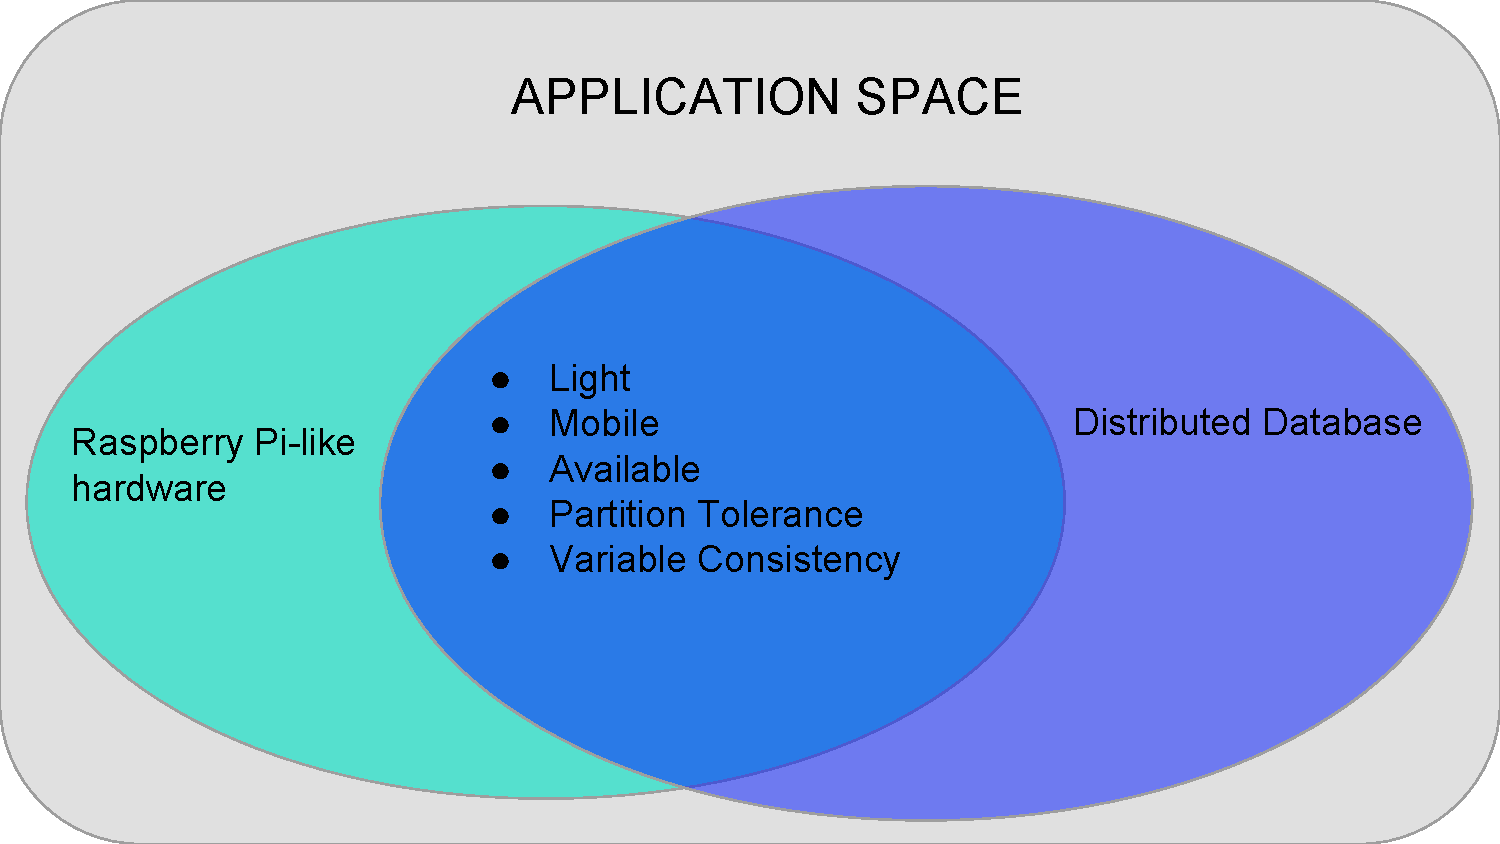
\includegraphics[width=7cm]{Figures/venn_diagram.pdf}
\caption{Venn Diagram of Application Space}
\label{fig:venn_diagram_of_application_space}
\end{figure}

\begin{figure}[h]
\centering
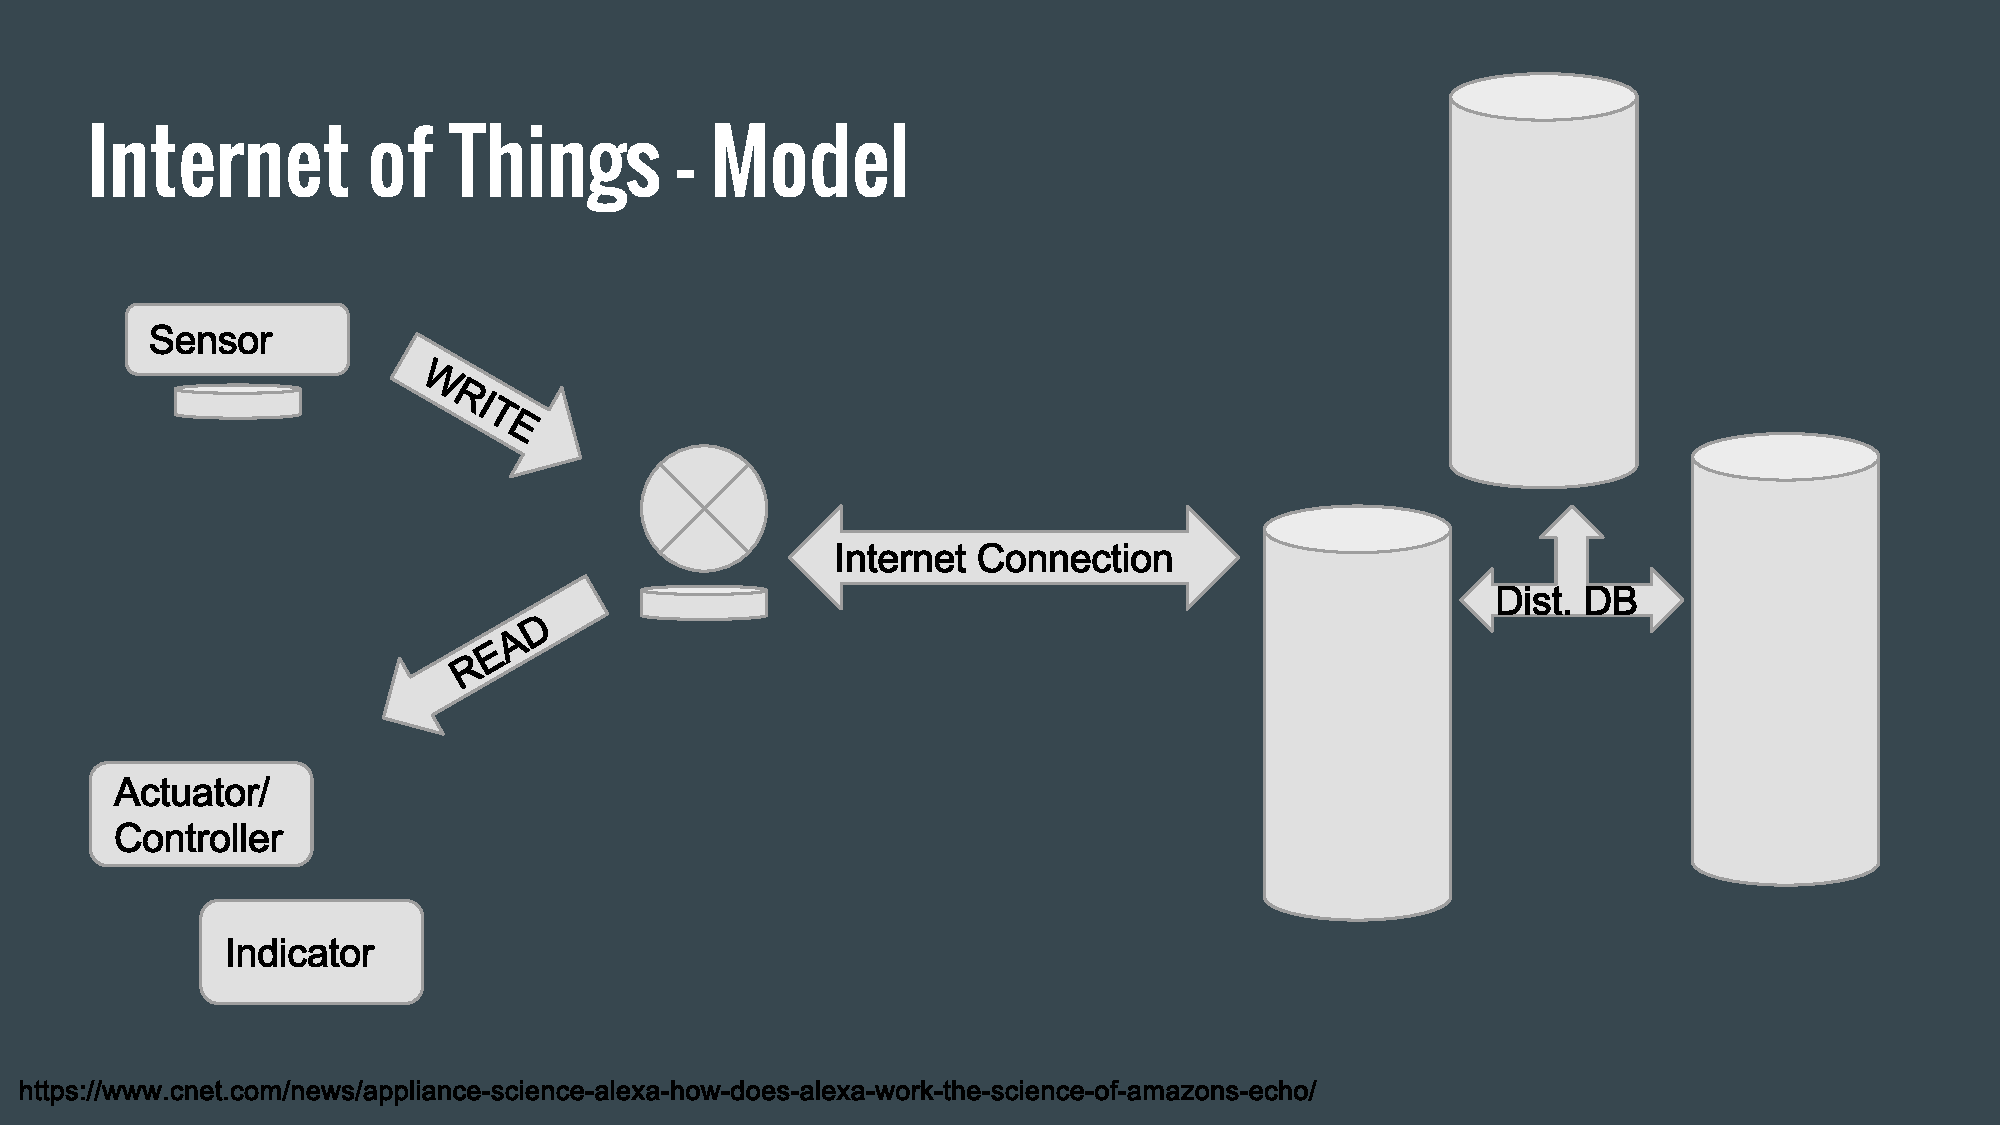
\includegraphics[width=7cm]{Figures/iot_original_model.pdf}
\caption{\gls{iot} Application...Although this isn't a rule, this represents a nominal "\gls{iot}" application.  Some measurement of interest, such as temperature is sensed, that raw data is stored and sent afar, and if desired, the user may also query for some kind of feedback or indication.}
\label{fig:iot_original_model}
\end{figure}

\begin{figure}[h]
\centering
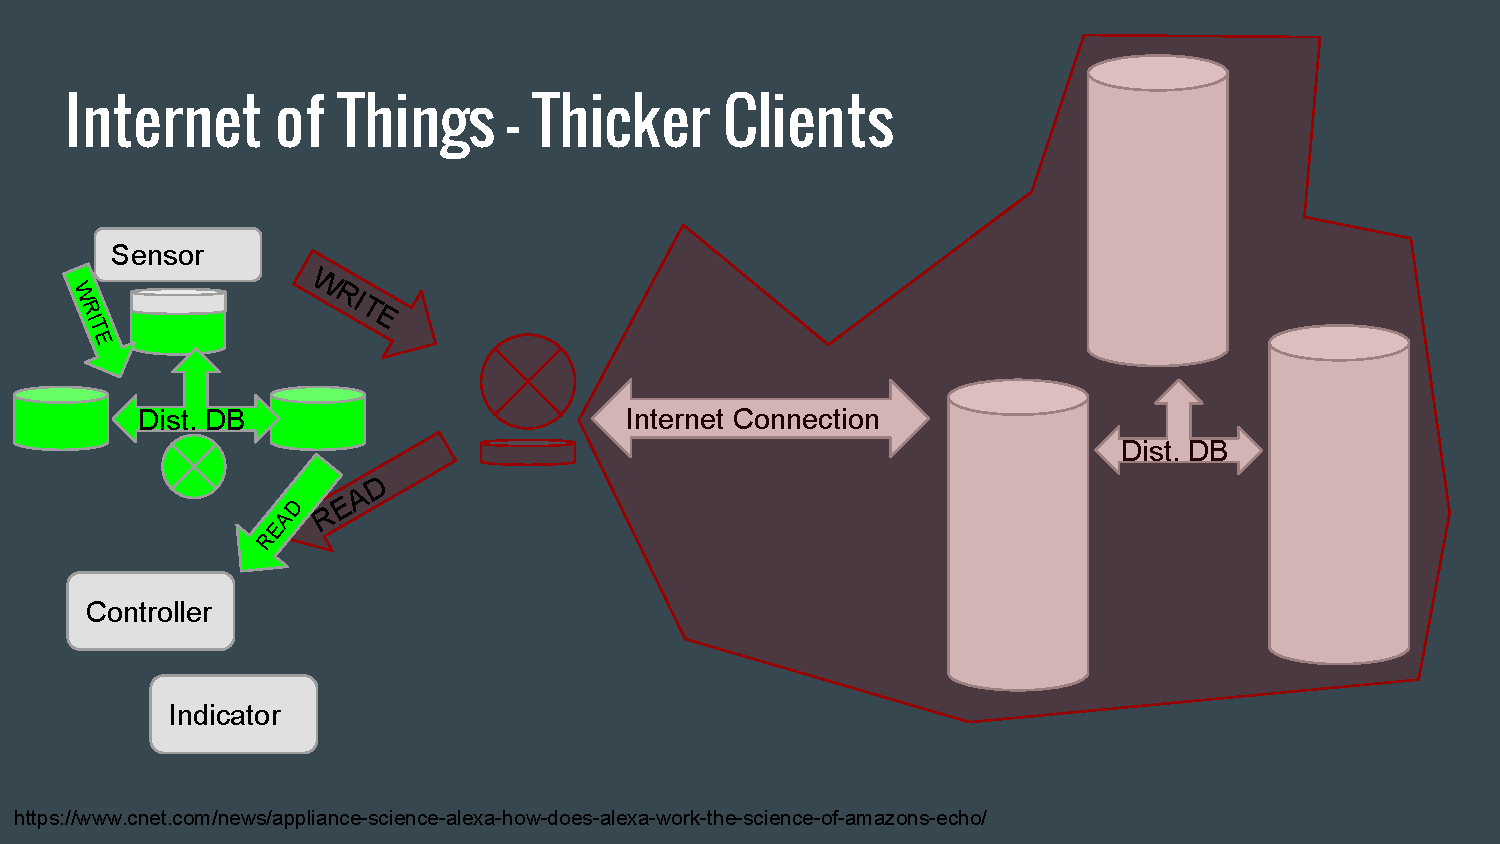
\includegraphics[width=7cm]{Figures/iot_modified.pdf}
\caption{\gls{iot} Application with Thicker Clients...Depending on the application, using a distributed database on thicker clients in-situ may suitably replace a remote database operating in a remote location.  From an operational standpoint, the pipeline may be unreliable, resulting in a loss of data.  From a security standpoint, this pipeline may be subject to undesired third-party monitoring.}
\label{fig:iot_modified}
\end{figure}

\label{where a distributed database fits in}

At the time of this writing, Cassandra, or other distributed databases, is used as a back-end database operating on powerful, but stationary nodes.  This paper explores the idea of moving toward a more in-situ database, where the sensing nodes may also contain serve as mechanisms for storage and do not require a pipeline to another datacenter, a pipeline that from an operational perspective, represents a single point of failure, or from a security perspective, a threat to privacy.

The next few sections map this general concept to some particular applications that are a bit easier to digest.

\subsection{WiFi Collection, Mapping and Analysis}
\subsubsection{WiFi Sniffing, Collection}
WiFi (802.11) sniffing, or war-driving, has been explored by a number of enthusiasts, both in and out of the academic realm.  These techniques for WiFi sniffing, at least on the front-end, is well-documented and thus represents a low barrier to entry for initial operations, often just requiring a specific WiFi chipset, such as the ALFA card, and open-source software.  One example that has been well-documented goes by the clever name of "Snoopy" \cite{SensePostFramework}.  Snoopy  provides a framework for collecting WiFi data and observing with another handy piece of software, Maltego.  Of course, a multitude of other software exists.  For example, one can sniff wireless traffic by using software Aircrack-ng \cite{Aircrack-ng} or Airsnort \cite{AirSnortHomepage}.  All this goes to show that it really doesn't take much to set up a sensor to get all the valuable information radiating throughout.  However, although sensing the data is easy, the subject of storage has not been fully explored with respect to the selling points mentioned above.  Investigating the limits of storage operations is key to unlocking realistic aspirations and application development.

\subsubsection{WiFi Mapping}
It may worth noting one off-shoot of the WiFi sniffing mentioned above: WiFi mapping.  There is much interest in WiFi mapping: Who doesn't want extra assurance of where they are in the world (especially if the GPS goes out)?  There has been much work done with respect to WiFi mapping.  Argos \cite{Rose2010MappingArgos} describes a similar system of a distributed system, but there is no mention of Cassandra or any distributed database, which may serve as an improvement on such a sensor network.  Wigle.net \cite{WiGLE:Mapping} is an aggregate map that distributes a smart-phone application to collect GPS coordinate-Access Point pairs, but relies on a central database, and has an unreliable user base and irregular sampling and update frequencies (Relying on the public will often do that, unfortunately.).  Heat Mapper \cite{HeatMapperOffices} is partially free and commercial software that can generate a heat map for a small room or office.  Wi2Me \cite{Castignani2012Wi2Me:Networks} performs this mapping as well, with an emphasis on performance and data throughput.  It uses an instance of SQLite to store the traces on the individual's smart-phone, but again, none of these make use of a distributed database like Cassandra as part of the sensor network.  Once again, this is a realm that may benefit integration with distributed databases, expanding the range possible node types, or both.  However, there are limits that have to be anticipated.  This paper aims to add a piece to that expectation management.

\subsection{WiFi/Wireless Crowd Detection}
There is also considerable interest in crowd detection and related data gathering.  Privacy implications notwithstanding, this kind of data can give a marketing-type a sense if certain areas are popular or versus other areas, or if certain paths are well-traveled or not.  The way WiFi broadcasts \gls{ssid}s in plain text, crowds can even be characterized as to whether individuals connect to similar access points or not.  The data can indicate whether you have a crowd of people from a certain country, a crowd of people who know each other or maybe just a crowd of strangers.  It can add assurance to more primitive forms of tracking, such as person-by-person registration.  Informally, some have even reported to make art exploiting this mechanism \cite{KeebleCasual2013}, and not surprisingly, there are numerous claims that members of the public are routinely tracked via commercial entities via WiFi \cite{HaighTrackingConnected}. There have been more academic efforts to track crowds as well, notably a university campus and a music festival in \cite{Bonne2013WiFiPi:Events} and an airport in \cite{Schauer2014EstimatingBluetooth}.  In \cite{Bonne2013WiFiPi:Events}, data travels through \gls{gsm} to a central node, but does not use any kind of distributed database, like Cassandra.  There are commercial entities that claim to track crowds and report data, namely "Bluemark" \cite{SchiphorstBlueInnovations}.  Here as well, a central server is utilized to collect the data.
Users then reportedly log into the web to view the metrics.  According to their marketing literature, they do use Raspberry Pi, but not for data storage. Paper \cite{ChilipireaPresumablyWiFi} used this product line for their tests. Although WiFi utilizes \gls{mac} addresses supposedly unique to each device, research has found that this leaves more to be desired for many applications, namely crowd-tracking.  For instance, some devices have been reported to change their MAC addresses \cite{ChilipireaPresumablyWiFi}.  There exist a number of papers that explore characterizing mobile devices and their users at the individual level \cite{Pang2007802.Fingerprinting, Chernyshev2016ServiceChallenges, Cunche2014LinkingRequests, Du2016EV-Linker:Matching, Cunche2012IRequests, Luzio2016MindRequests, Musa2012TrackingMonitors} and propose techniques to better prepare data for analysis \cite{ChilipireaPresumablyWiFi}.  What is clear in the subtext of all these papers, is that these types of application research can only benefit from a wider choice in nodes, and a wider choice storage options as well as a reasonable amount of foresight into their performance.  In all of these, however, distributing the stored data among the nodes, like with Cassandra is either not used or not mentioned.  Many utilize a central server that represents a single point of vulnerability.

\subsection{CBIR and others and summary statement on application space}
The motivation for WiFi mapping can also be extended to other types of mapping, such as \gls{cbir}.  Paving the way for feasible, desirable in-situ data storage increases the portability and development of these and many more applications.

The experiments that follow read and write random data in the context of a meaningless, and rather ho-hum schema, but the experiments were done with the following in mind: A schema supporting any of these up-and-coming applications could be substituted in instead, and ideally with predictable results.

\section{Representative Technologies}

\subsection{Cassandra}
\label{Cassandra}
%NEED FOR DISTRIBUTED DATABASE
A distributed database offers a trade space among consistency, availability, and partition tolerance.  Mostly this means that a system of nodes can still operate as expected even if there is a loss of one or two nodes.  There is no shortage of distributed databases to choose from, but Cassandra is widely used  and is known to have a high write throughput \cite{Cooper2010}.  Cassandra specifies the “latest” versions of both “Java 8” and “Python 2.7”.  In turn, Java can run on Windows, Mac OS X, Linux, and Solaris \cite{CassandraHardwareWiki}.

%SELECT THE REPRESENTATIVE – CASSANDRA AND WHY?
Cassandra is a widely used distributed \gls{nosql} database with many use cases \cite{Lakshman2010CassandraSystem} and boasts a high write throughput. Not only has Cassandra been reportedly been used in practice \cite{ApacheCases}, but has been, using the Yahoo Cloud Services Benchmark \cite{YahooBenchmark}, formally evaluated in scholarly literature against other databases such as MongoDB and proposed as the NoSQL database of choice in the Internet of Things and distributed sensor networks \cite{Abramova2013NoSQLCassandra}.

%SET OF HARDWARE/OS THAT SUPPORT CASSANDRA
If possible, it is important to get realistic expectation from available specifications whether or not the database of interest, Cassandra, would be supported by the node of interest, in this case Raspberry Pi. At the time of this writing, Cassandra specifies it is supported by the “latest” versions of both “Java 8” and “Python 2.7” \cite{CassandraHardwareWiki}.  In turn, Java can run on Windows, Mac OS X, Linux, and Solaris.  Raspbian, a Linux-based operating system, can be run on Raspberry Pi.  In addition, there have been credible claims of Cassandra being used on Raspberry Pi \cite{VanRyswykMulti-DatacenterPis,SercelCassandraMedium}, but to the author's knowledge, no white paper with the details exists.

This author's interest in Cassandra lies in the fact that Cassandra is a distributed database used in practice for cloud computing.
Although it describes itself as a \gls{nosql} database, the interface allows for \gls{sql} commands and has a Python \gls{api}.
Cassandra allows for configuration of distributed systems parameters, such as replication factor, but detailed knowledge of distributed systems protocols is not critical for operation.

%But in a way, this is the simplified version of the application that this is testing.
The aim of this paper is to examine Cassandra's performance coupled with a simplified Wi-Fi collection and analysis application, where the nature of link nodes may be less reliable than wired Ethernet.

From an experimental standpoint, the distributed nature of a Cassandra "keyspace" lies in four parameters \cite{CassandraDummies}: cluster size (the number of nodes), replication factor (configured in software), write level (configured in software), and read level (configured in software).
As alluded to in section \ref{Factors Held Constant}, these factors will be held constant for this experiment.

\subsection{Raspberry Pi 2}

The Raspberry Pi 2 (Model B) \cite{RaspberryB} is a low-cost computer designed sold from the United Kingdom.
It can be described as a motherboard for a about the size of a 3x5 index card and has been available since February 2015.
This experiment is interested in the Raspberry Pi 2 as a representative of the low-cost hardware domain, which implies low cost, low power consumption, and low in terms of size and weight.

This author's interest in the Raspberry Pi 2 is that its ARM Cortex-A7 processor and 1GB \gls{ram} \cite{RaspberryB} makes it a key representative of the low-cost hardware domain and the \cite{iot}.
The Raspberry Pi 2 has cost as low as 35 \gls{usd} \cite{RaspberryPi}.
It is lightweight and has limited power consumption \cite{RaspberryB}.
Constraints on size, weight, power, and cost can all be barriers to entry for applications seeking computing nodes.

Expanding this experiment, to say the BeagleBone black \cite{BeagleBoard.orgBlack}, is in touch with the spirit of this experiment but outside the scope of this paper.  A number of possible alternatives is listed in Table \ref{table:low_cost_hardware}

\begin{table}
\begin{tabular}{|| p{2cm} | p{4cm} | p{2cm} | p{3cm} | p{1.5cm} ||}
\toprule
 Name	& CPU	& RAM &	DISK &	Price \\
\midrule
Banana Pi M3 &	Octa-core 1.8GHz CPU &	2 GB RAM &	8 GB eMMC flash storage	& 73.00 \\
\hline
CHIP &	R8 1GHz &	512 MB &	4 GB	& 9.00 \\
\hline
VoCore &	360 MHz MIPS CPU &	32 MB &	8 MB Flash	& 20.00 \\
\hline
Arduino INDUSTRIAL 101 &	Atheros AR9331 Processor &	64 MB &	16 MB Flash	& 40.00 \\
\hline
NanoPi 2 Fire &	Samsung S5P4418 quad-core ARM Cortex-A9, 1.4 GHz & unk &	1 GB MicroSD card & 22.99 \\
\hline
NanoPC-T3 &	Samsung S5P6818 octa-core ARM Cortex-A53 up to 1.4 GHz & 1-2GB of RAM & 8GB of flash storage & 60.00 \\
\hline
Intel Edison with Kit for Arduino & Dual-core, dual-threaded Intel Atom CPU with a 32-bit Intel Quark microcontroller & 1GB of RAM & 4GB of flash storage & 92.00 \\
\hline
cloudBit & Freescale i.MX23 ARM926EJ-S processor & 64MB of RAM & 4GB SD Card & 59.95 \\
\hline
Parallella & 16-core Epiphany RISC SOC & unk & unk & unk \\
\hline
Zynq SOC & (FPGA + ARM A9) & 1GB SDRAM & Micro-SD storage & 99 \\
\hline
PixiePro & Freescale i.MX6Q Soc Quad Core ARM Cortex-A9 up to 1GHz & 2GB of RAM& SD Card	& 129.95 \\
\hline
Raspberry Pi & 900 MHz quad-core ARM Cortex-A7 CPU & 1GB RAM & MicroSD Card & 35.90 \\
\bottomrule
\end{tabular}
\caption{Raspberry Pi Alternatives, Depending on Application}
\label{table:low_cost_hardware}
\end{table}

%\subsection{Wireshark software and PCAP files}

%A PCAP file stores networking packets and is a "main capture file format" \cite{tcpdumpTcpdump/LibpcapRepository}.
%In this case, the PCAP file is used as a tool in the benchmark, a means to an end.

%Commonly associated with PCAP files, and used by this author is the Wireshark software \cite{WiresharkDeep.}.
%This was used to view and confirm that the PCAP files were generated to taste.

%Not even a vague familiarity of these is needed to understand the experiment, but they are a fundamental part of the custom benchmark of choice. 
\chapter{Cassandra Pilot Tests}

Despite its popularity, the \gls{ycsb} is not the only benchmark in existence for distributed databases. Although using a commonly used and trusted database benchmark mitigates some risk as opposed to one that is hardly used, relying on multiple, independent instruments always reduces measurement risk.

Cassandra comes with its own stress-testing tool, denoted 'cassandra-stress' \cite{DatastaxTheTool} in the tarball installation.  By all appearances, it is designed to give an operator an idea of how Cassandra performs over time on a given hardware setup.  But, it also allows an operator to vary a limited set of configuration parameters with each command line execution.  Naturally, this stress testing tool does not allow one to compare Cassandra to a competitor, hence the \gls{ycsb} in the main section of this paper, but Cassandra-stress may also serve as a check on the \gls{ycsb}.

One thing to note about the main results of this paper is that Cassandra is running with default parameters with no intention of running optimally.  In fact, Cassandra has so many versions and configuration parameters, it's almost guaranteed that one is running Cassandra sub-optimally.  This section does not seek to run Cassandra optimally, but rather explore the sensitivity of Cassandra when its configuration parameters are altered.  If the results achieved with default parameters seem too precise, these experiments will further shape the expectations one might have improving the absolute results achieved in the main work.

Once the tests were run, the results required additional processing.  Normally, when one invokes the cassandra-stress, the output is placed into an \gls{html} file that displays a graph with time as the independent variable across the x-axis.  Since this the, a Python script was written to strip the data from the generated \gls{html} file to be further processed.

\section{Experimental Setup}

The set-up follows the guidelines established in the main methodology. The set of experiments described in this section explored how Cassandra performs. Here a cluster of 3 Raspberry Pi 2 nodes was used. The tarball version of Cassandra version 3.9 was downloaded and installed.

\section{Variance in Nature of the Links with Compression Algorithms}

\begin{figure}[h]
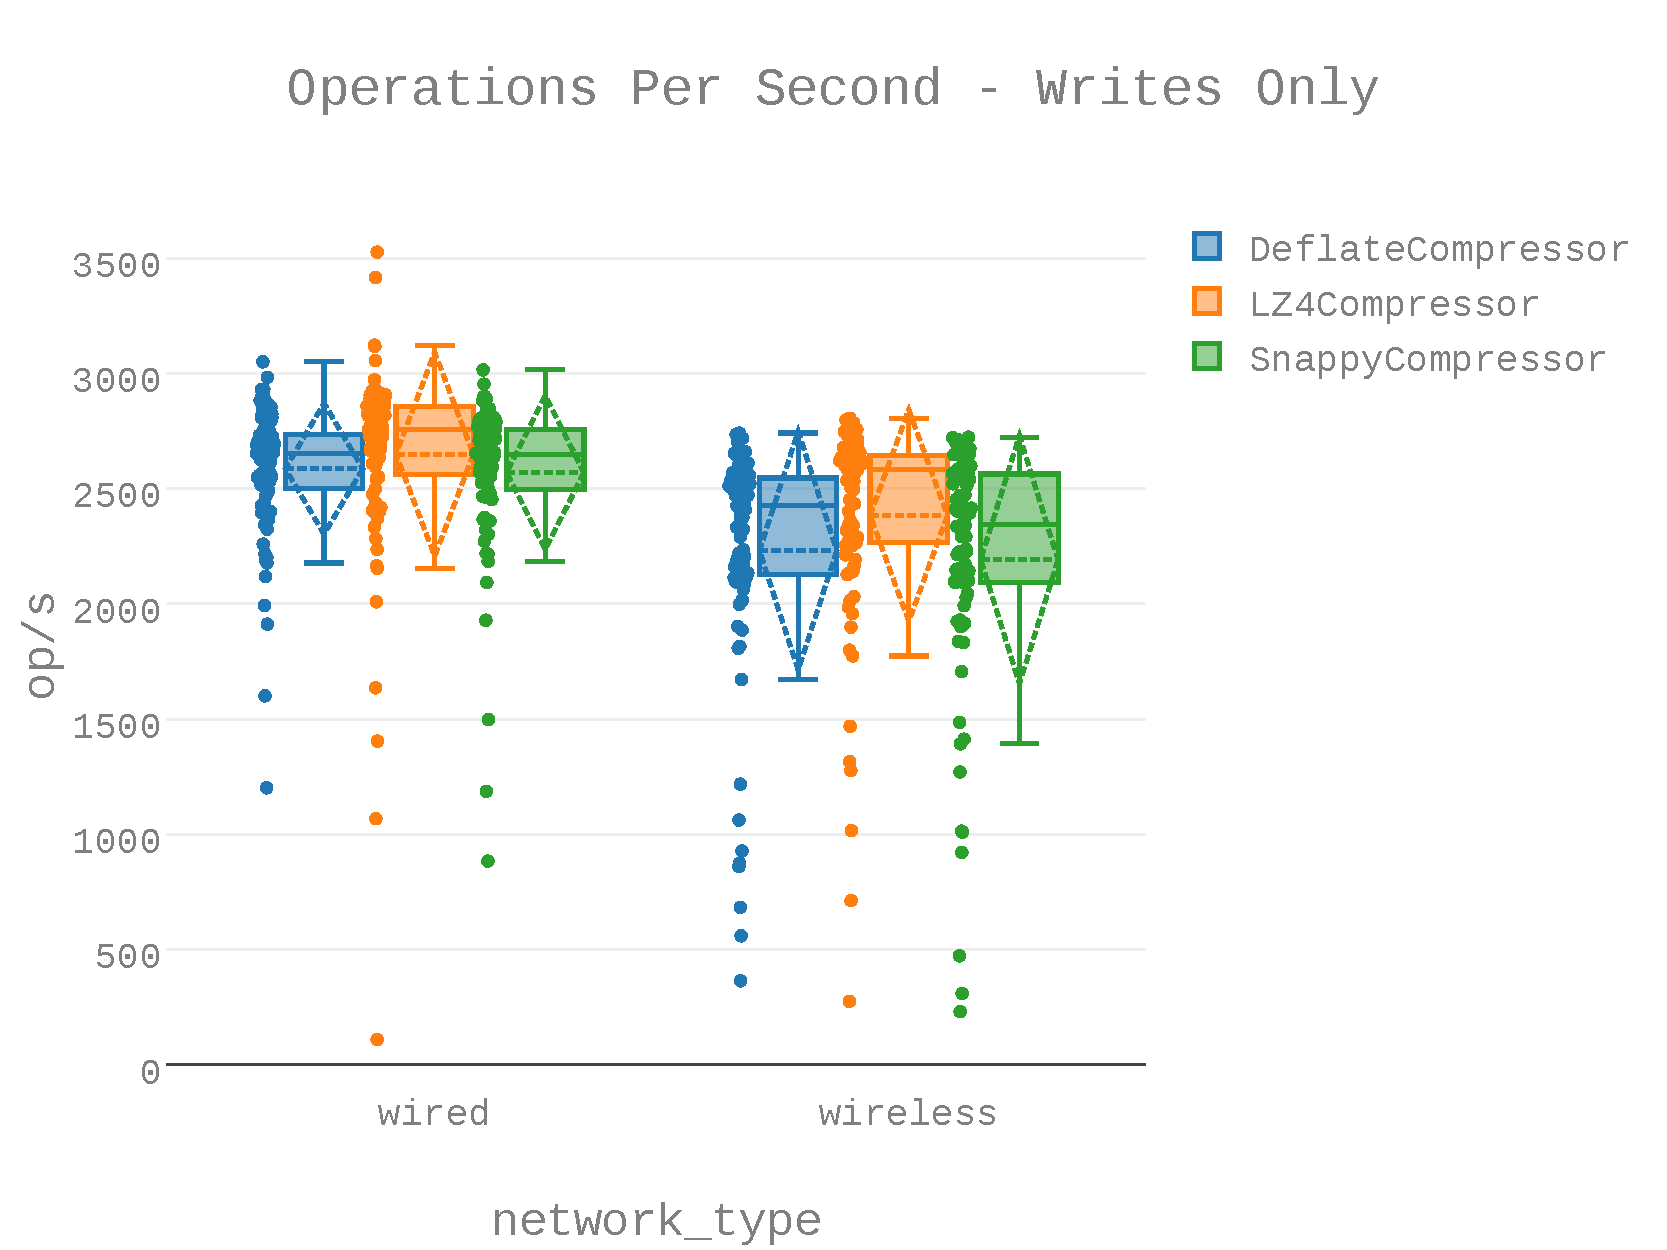
\includegraphics[width=7cm]{Figures/figures-cs1_fig1.pdf}

\caption{Varying Compression Methods: Writes}

\label{fig:res}
\end{figure}
	The above box plot shows the effect of varying compression strategies for a given configuration on a pure write load as load-tested through the cassandra-stress module.  In the left, wireless 802.11 links were used.  On the right, wired Ethernet links were used.  A one-way analysis-of-variance (ANOVA) may be able to test whether there is a significant differential between either of these two means, but from visual inspection, one could say that for a given configuration and a write-heavy load, varying the compression strategy does not have a large effect on performance as far as writes per second.
\begin{figure}[h]
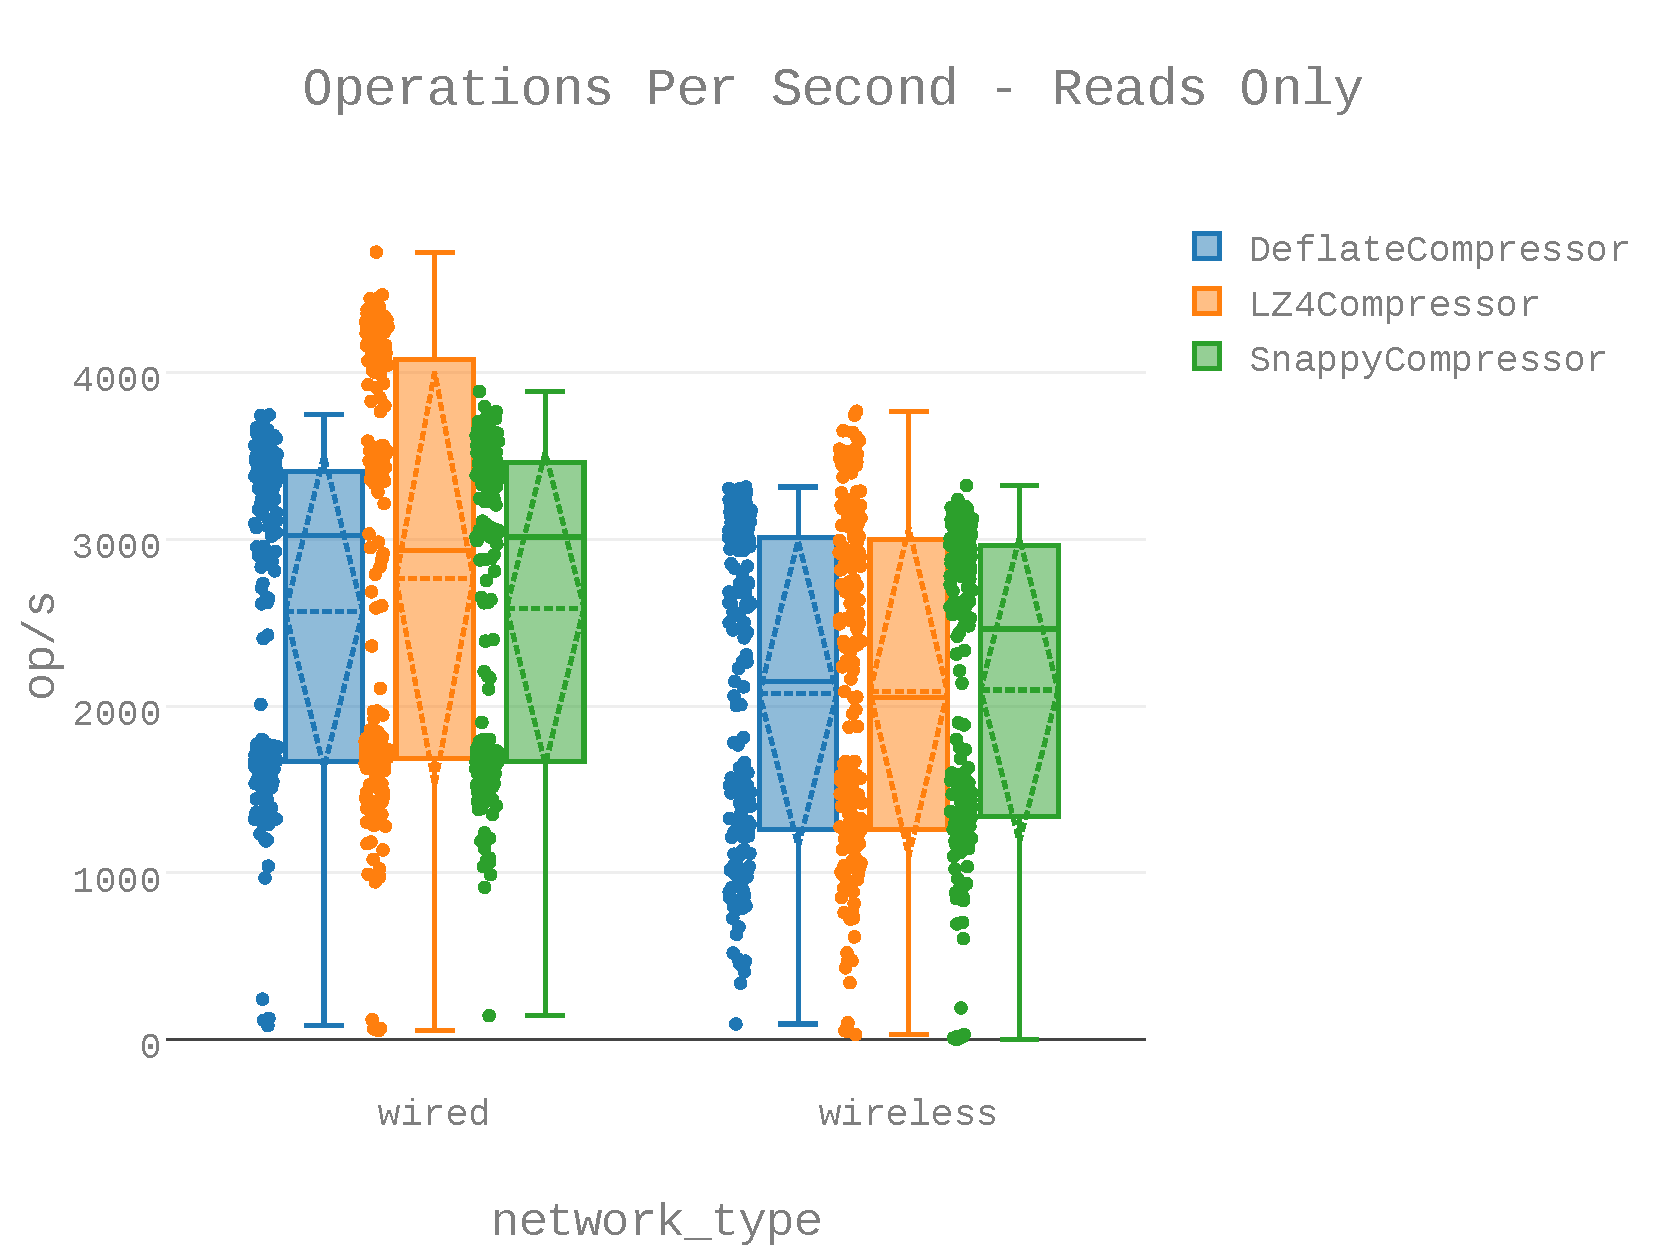
\includegraphics[width=7cm]{Figures/figures-cs1_fig2.pdf}

\caption{Varying Compression Methods: Reads}

\label{fig:res}
\end{figure}
	To represent a read-heavy load, a pure read load was put through cassandra-stress, varying both compression strategies and wireless versus wired link nature.  In the wired domain (right), a hierarchy seems to emerge.  The LZ4 compression algorithm renders the most reads per second, followed by the Snappy compression algorithm, and finally the Deflation compression algorithm.  This correlates with the expectations put forth by the manual, as the selection in compression algorithms represents a trade-off between speed (operations per second) and compression effectiveness (storage in bytes) for the user.  Such a hierarchy does not seem to emerge from the wireless links, but there is no known explanation for this at this time.  Increased variation is not unexpected, perhaps due to \gls{ism} band interference, but one would expect the means to follow a similar pattern.  A series or regressions or multi-factor \gls{anova} test could be utilized to see if the graph is deceiving and the means truly are significantly different, but is not merited at this time.

\begin{figure}[h]
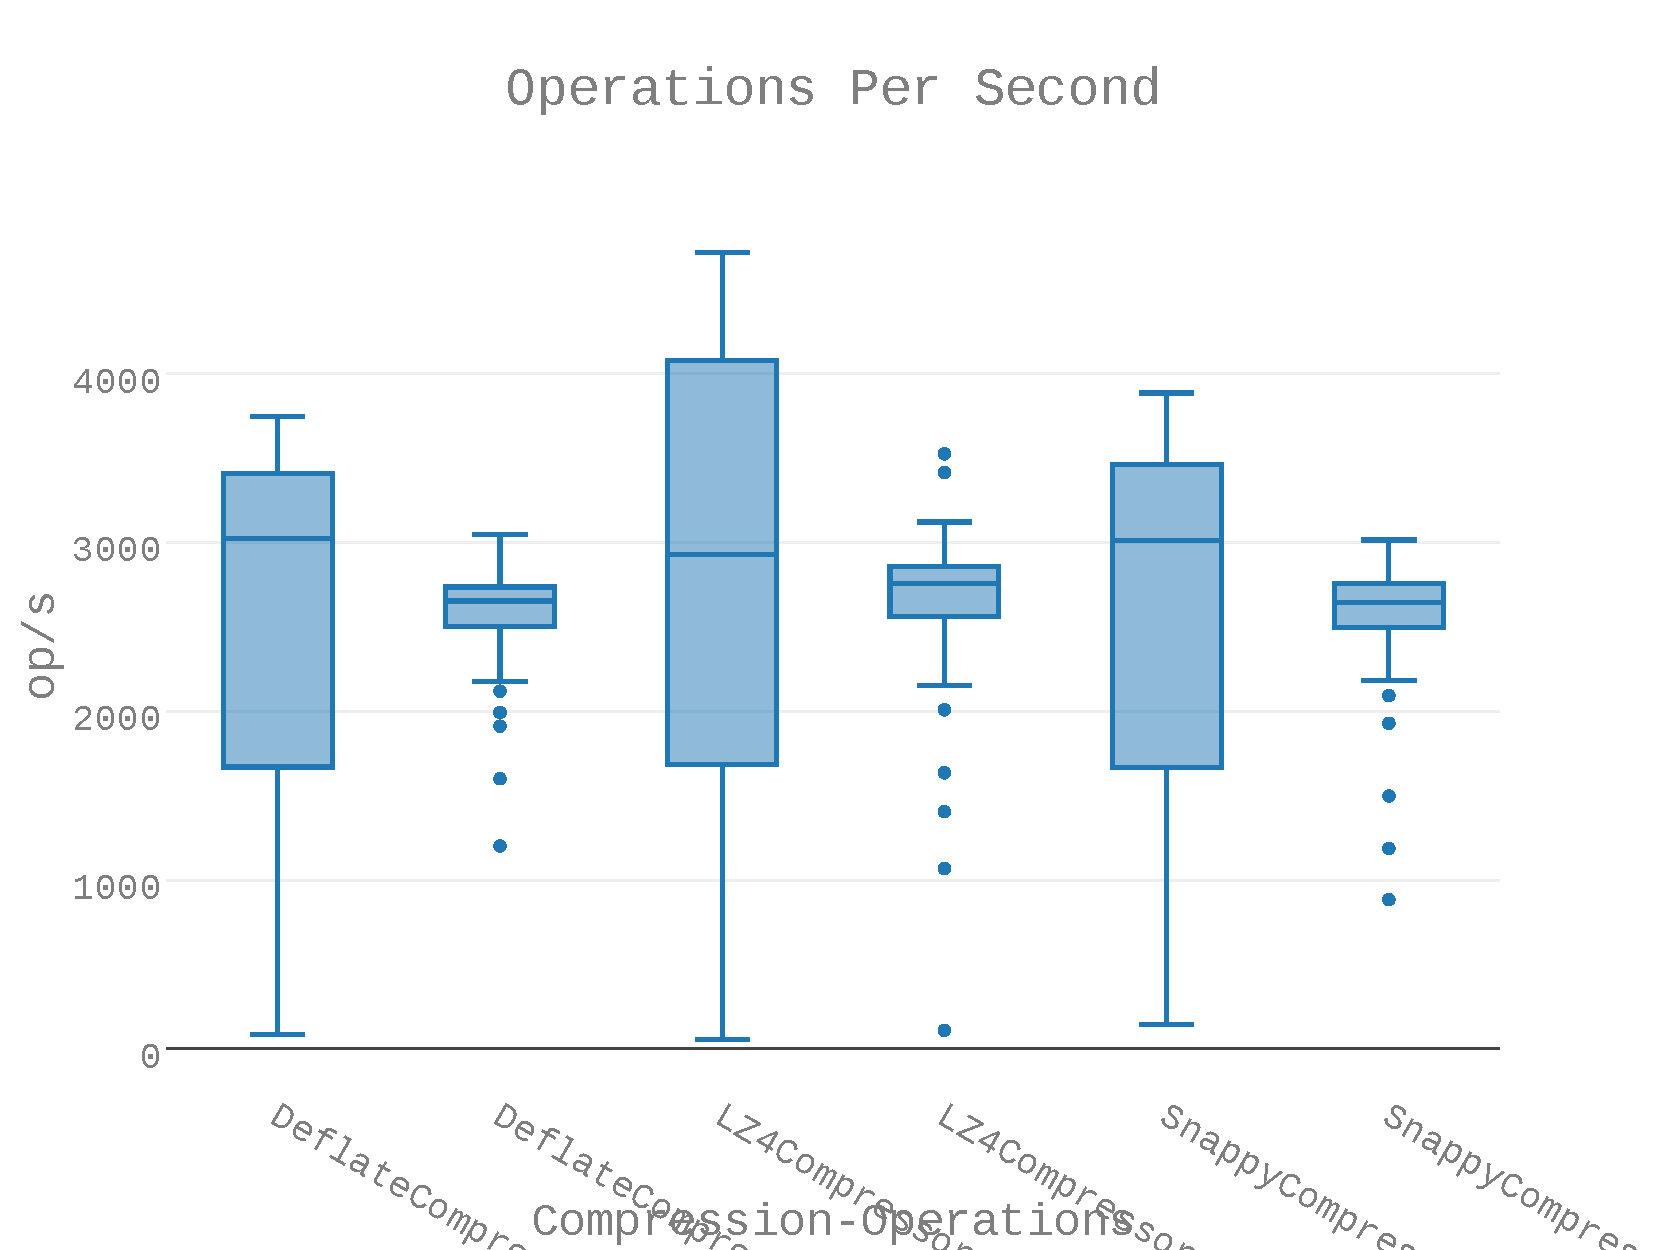
\includegraphics[width=7cm]{Figures/figures-cs1_fig3.pdf}

\caption{Compression Methods Sorted by Best Performance: Wired \gls{lan} Case}

\label{fig:res}
\end{figure}
	The above box-plot shows, for wired, how performance can vary with respect to different compression strategies and loads.  For reads, the compression strategy hierarchy seems to correlate with what is expected from reading the manual: the LZ4 algorithm renders highest performance in operations per second, followed by the Snappy algorithm, then the Deflate algorithm.  For writes, the hierarchy continues but is less pronounced.  

\begin{figure}[h]
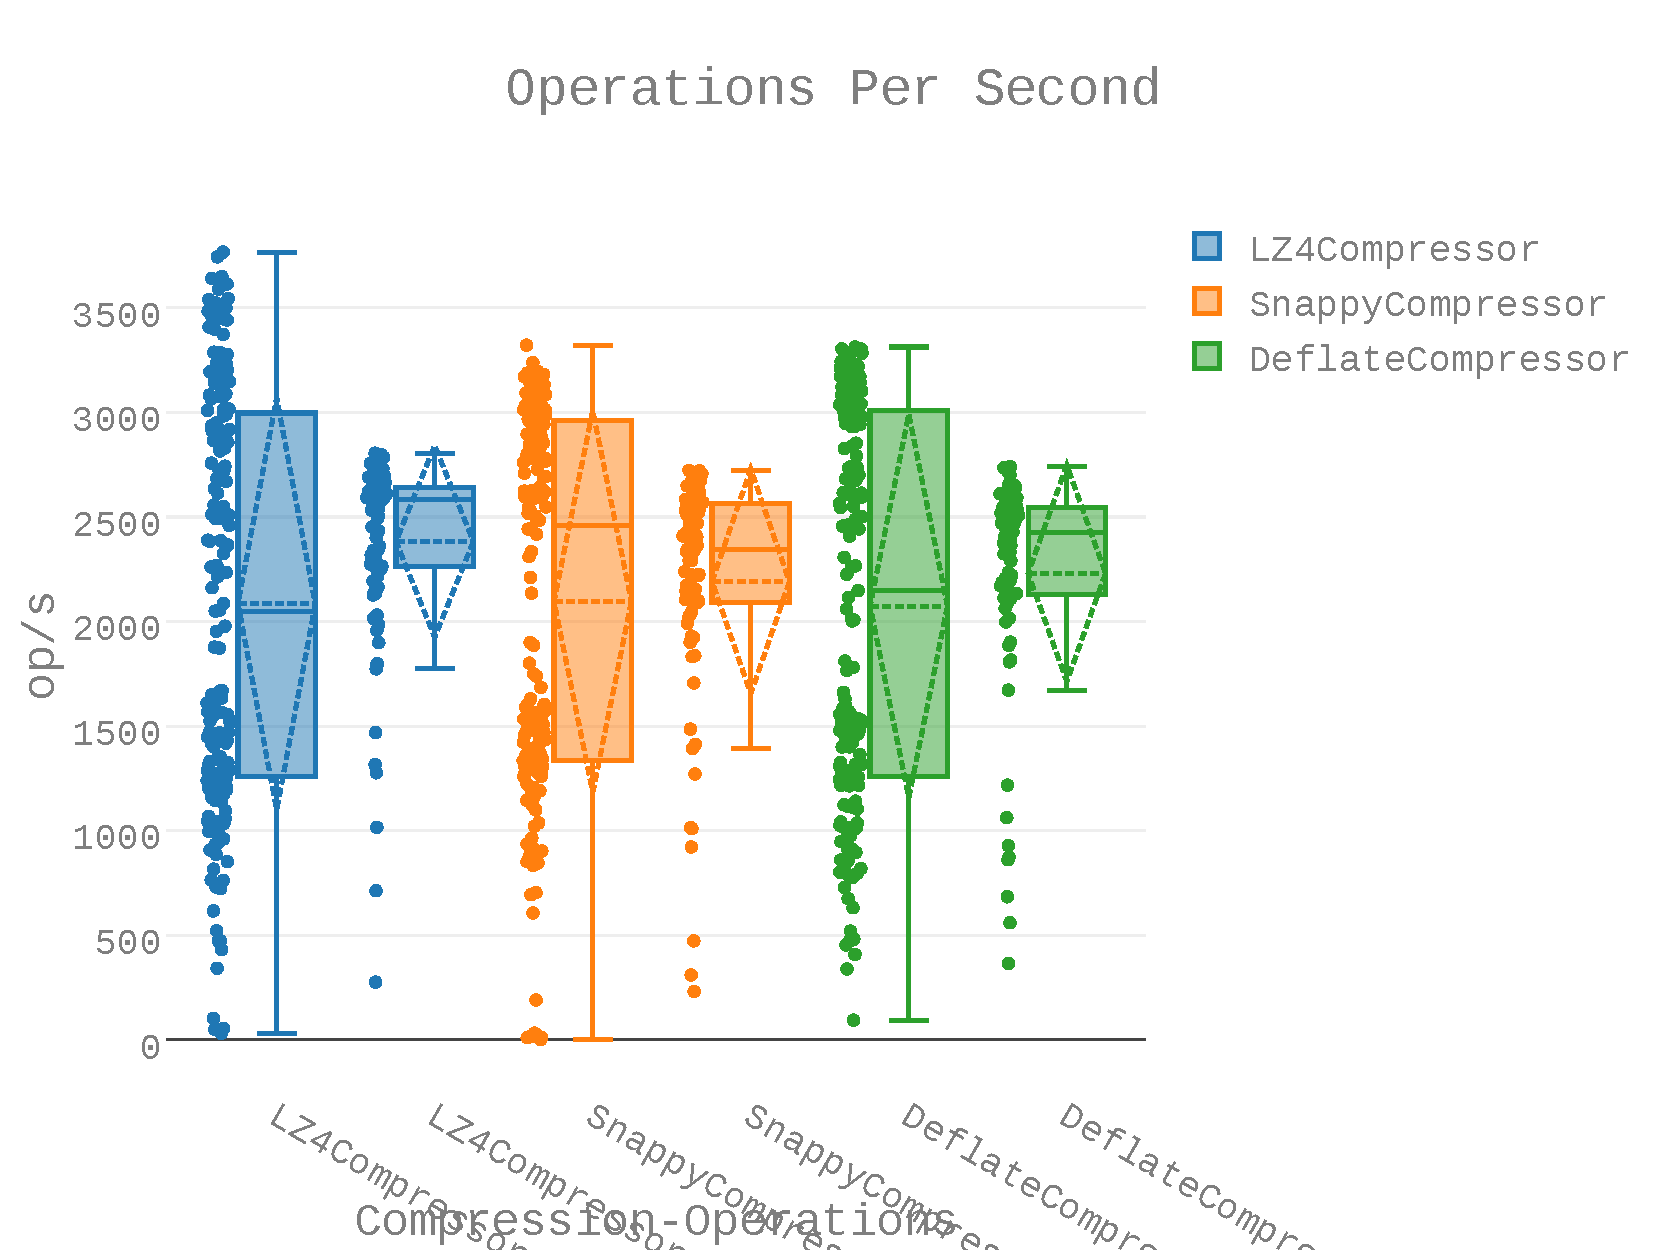
\includegraphics[width=7cm]{Figures/figures-cs1_fig4.pdf}

\caption{Compression Methods Sorted by Best Performance: Wireless \gls{lan} Case}

\label{fig:res}
\end{figure}

	For the wireless links, the LZ4 algorithm seems to remain the highest performer, but the Deflate and Snappy algorithms seem to exchange places in the hierarchy, both for reads and for writes.  The means, shown as the dashed horizontal lines are very close together on both counts, so a hypothesis that the switch is not significant may be of merit.  The main thing that this graph shows is that at least in one test, the wireless links allowed for reasonably similar performance levels across compression strategies and loads.  To a potential application in the \gls{iot} domain, this may imply that one is not sacrificing much in the manner of operations per second by configuring Cassandra to employ a more effective compression strategy, such as the Deflate algorithm.



\chapter{Methodology}

\section{Overview of Similar Experiment}

Although this work has a slightly different aim than \cite{Abramova2014}'s stated purpose, this paper aims to follow \cite{Abramova2014}'s methodology closely enough as to anchor its results to a cross-section of similar work that has been done.  This work assumes that an in-situ storage application in the realm of \gls{iot} implies a small database, in this case represented by 1 million records, as opposed to 10 million or 100 million or more.  Although Abramova’s paper seems to imply there is feasibility for large database with many, many nodes given the right balance, this work focuses more on the initial impact to performance of introducing less-capable hardware in order to lighten costs or actual physical weight for an application that would see this as a benefit.

Using standard workloads A, C, and E from the popular \gls{ycsb}, the authors of \cite{Abramova2014} examined and evaluated Cassandra’s scalability over “database [sizes] and cluster sizes” \cite{Abramova2014}.  The authors found that this trend, depicted in Figures \ref{fig:wla_fig1}, \ref{fig:wlc_fig1}, and \ref{fig:wle_fig1} did not necessarily hold true across database sizes, that in fact for larger database sizes of 10 million and 100 million records, 3 node clusters performed better than both a single node cluster and a 6-node cluster.  The authors concluded that for sufficiently small databases, which is the likely case for \gls{iot}, more nodes imply more time to execute, which overwhelms any advantageous parallelism that may ensue with increasing nodes.

Because there are so many variables that can be at work, this work aims to anchor its results by replicating part of Abramova’s study.  The extent of the details of the network in \cite{Abramova2014} is detailed below:  

"The characteristics of nodes used are, as follows: Node 1 – Dual Core (3.4 GHz), 2GB RAM and disk with 7200 rpm; Node 2 – Dual Core (3.4 GHz), 2GB RAM and disk with 7200 rpm; Node 3 – Dual Core (3.4 GHz), 2GB RAM and disk with 7200 rpm; Node 4 – Dual Core (3.0 GHz), 2GB RAM and disk with 7200 rpm; Node 5 – Dual Core (3.0 GHz), 2GB RAM and disk with 7200 rpm; Node 6 – Virtual Machine with one Core (3.4 GHz), 2GB RAM and disk with 7200 rpm." \cite{Abramova2014}

The results of Workloads A, C, and E in \cite{Abramova2014} are depicted in Figures \ref{fig:wla_fig1}, \ref{fig:wlc_fig1}, and \ref{fig:wle_fig1} respectively, all depicting a positive correlation between execution time and the number of nodes.  The actual values are depicted in \ref{table:previous_paper_results}

\begin{table}
\begin{center}
 \begin{tabular}{||c c c||} 
 \hline
Nodes & Workload & [OVERALL] RunTime(ms) \\ [0.5ex] 
 \hline\hline
1 & a & 58430\\ 
 \hline
3 & a & 65650\\ 
 \hline
6 & a & 87310\\ 
 \hline
1 & c & 88000\\ 
 \hline
3 & c & 90210\\ 
 \hline
6 & c & 118090\\ 
 \hline
1 & e & 223180\\ 
 \hline
3 & e & 330820\\ 
 \hline
6 & e & 404660\\ 
 \hline
\end{tabular}
\end{center}

\caption{Results from \cite{Abramova2014} for 1 million record size database}
\label{table:previous_paper_results}
\end{table}

\begin{figure}[h]
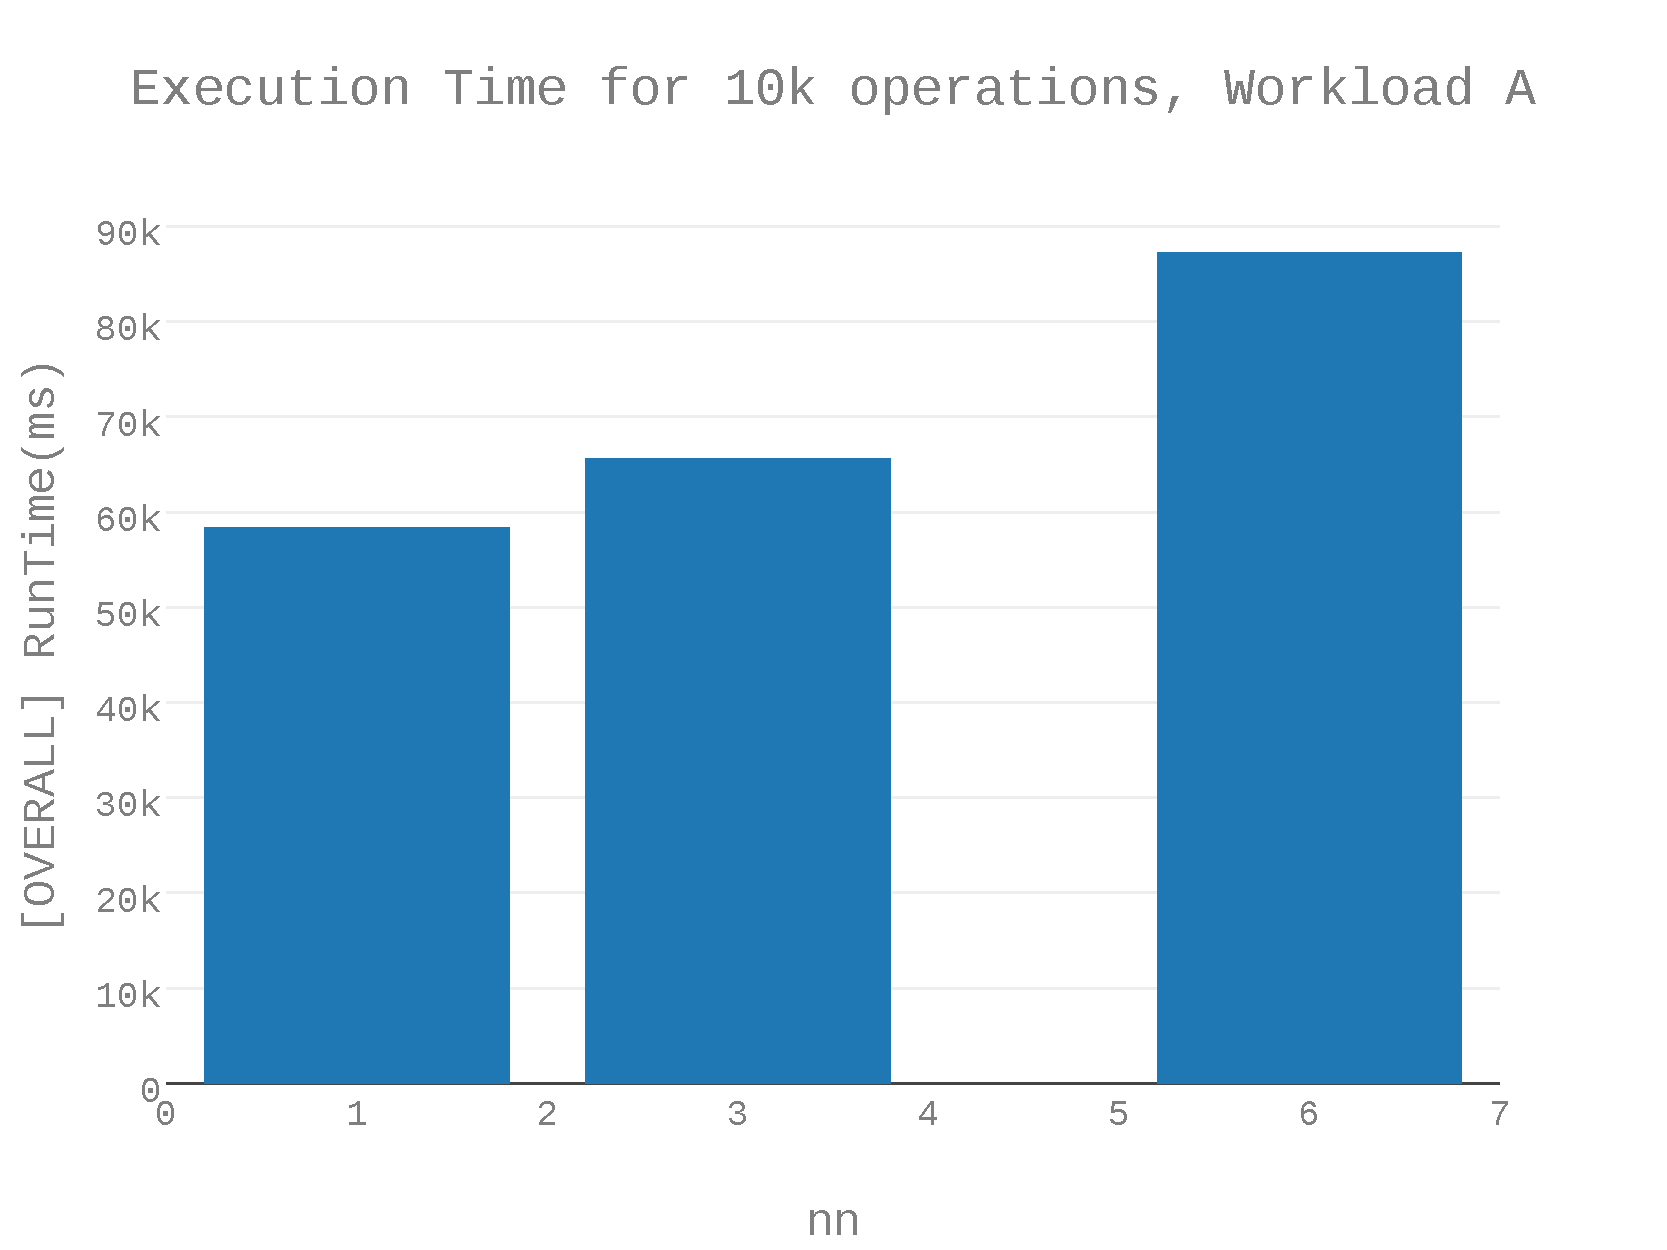
\includegraphics[width=3.5in]{Figures/figures-wla_fig1.pdf}

\caption{Cross Section of Results Imported from \cite{Abramova2014}.  This figure shows the execution time reported for 10,000 operations of Workload A over three given configurations: a network with only one (1) node, a network with 3 nodes, and a network with 6 nodes.}

\label{fig:wla_fig1}
\end{figure}

\begin{figure}[h]
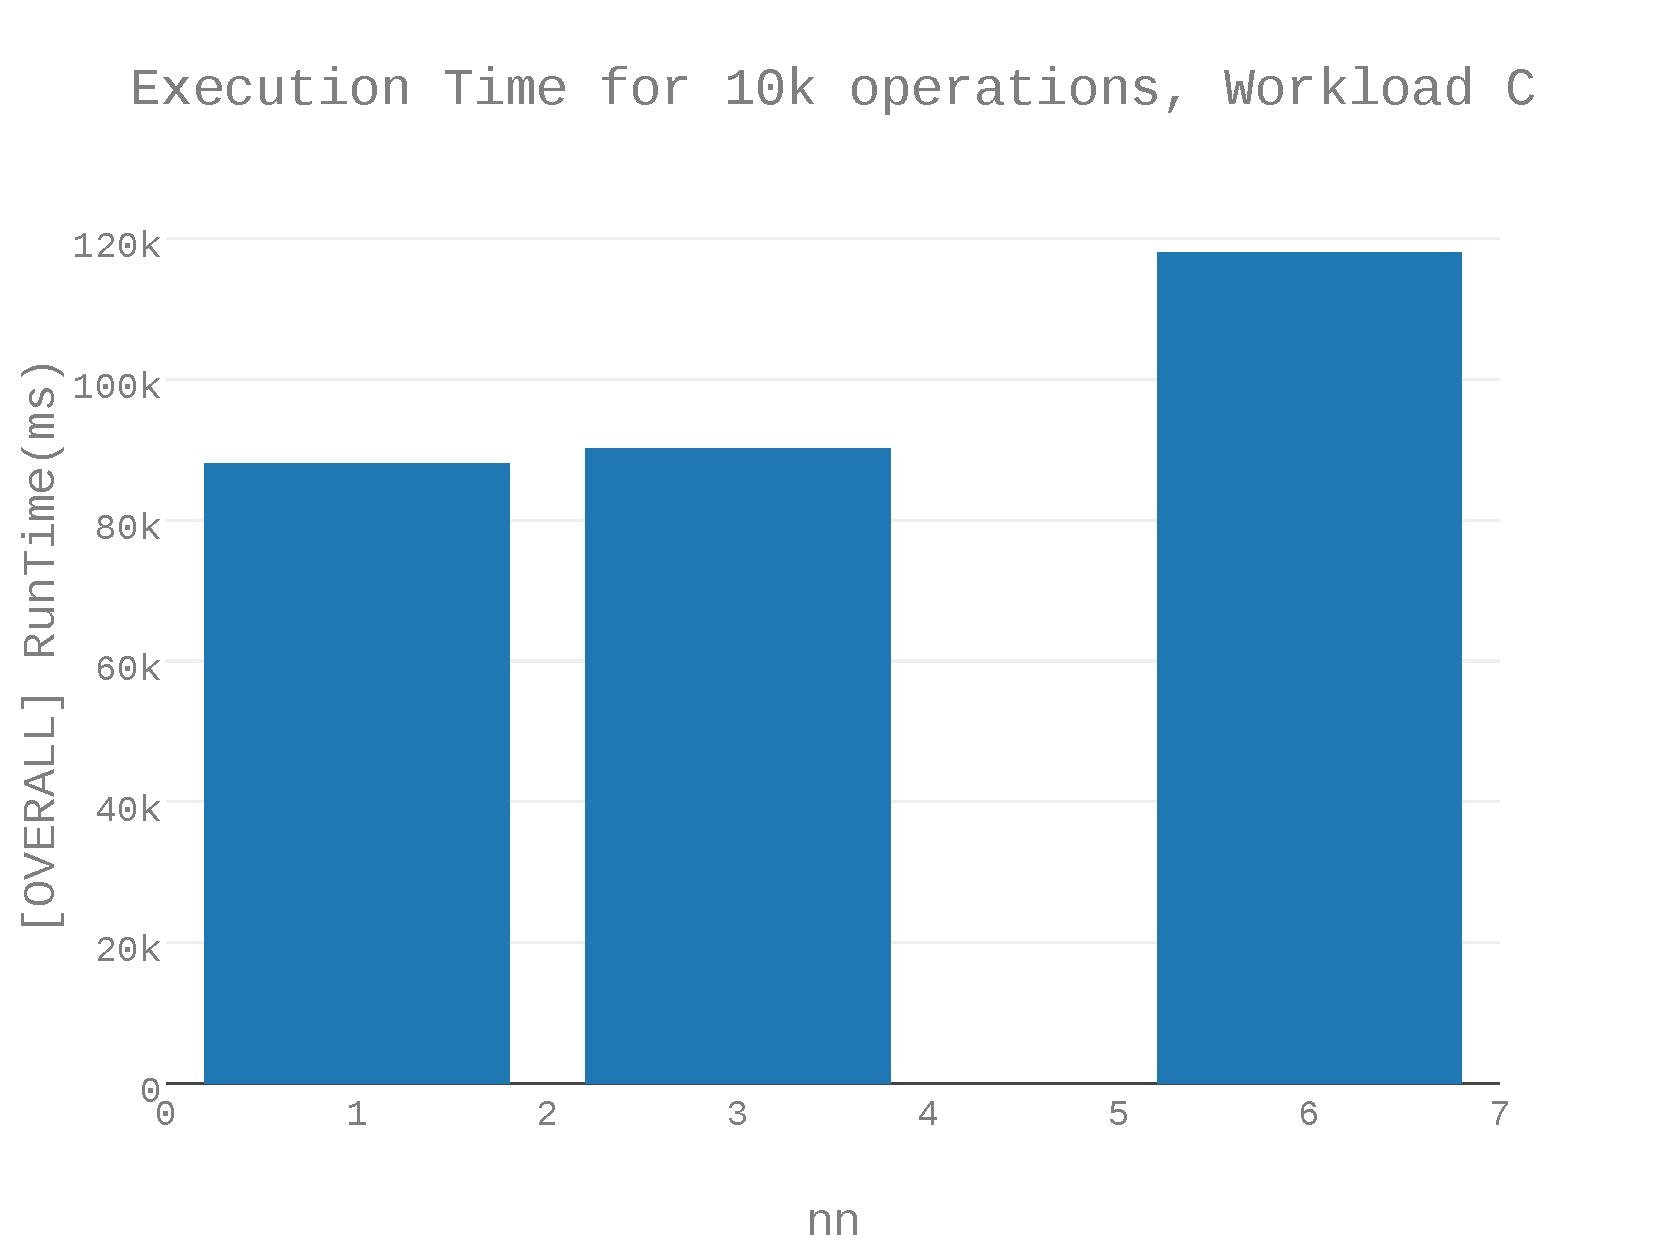
\includegraphics[width=3.5in]{Figures/figures-wlc_fig1.pdf}

\caption{Cross Section of Results Imported from \cite{Abramova2014}.  This figure shows the execution time reported for 10,000 operations of Workload C over three given configurations: a network with only one (1) node, a network with 3 nodes, and a network with 6 nodes.}

\label{fig:wlc_fig1}
\end{figure}

\begin{figure}[h]
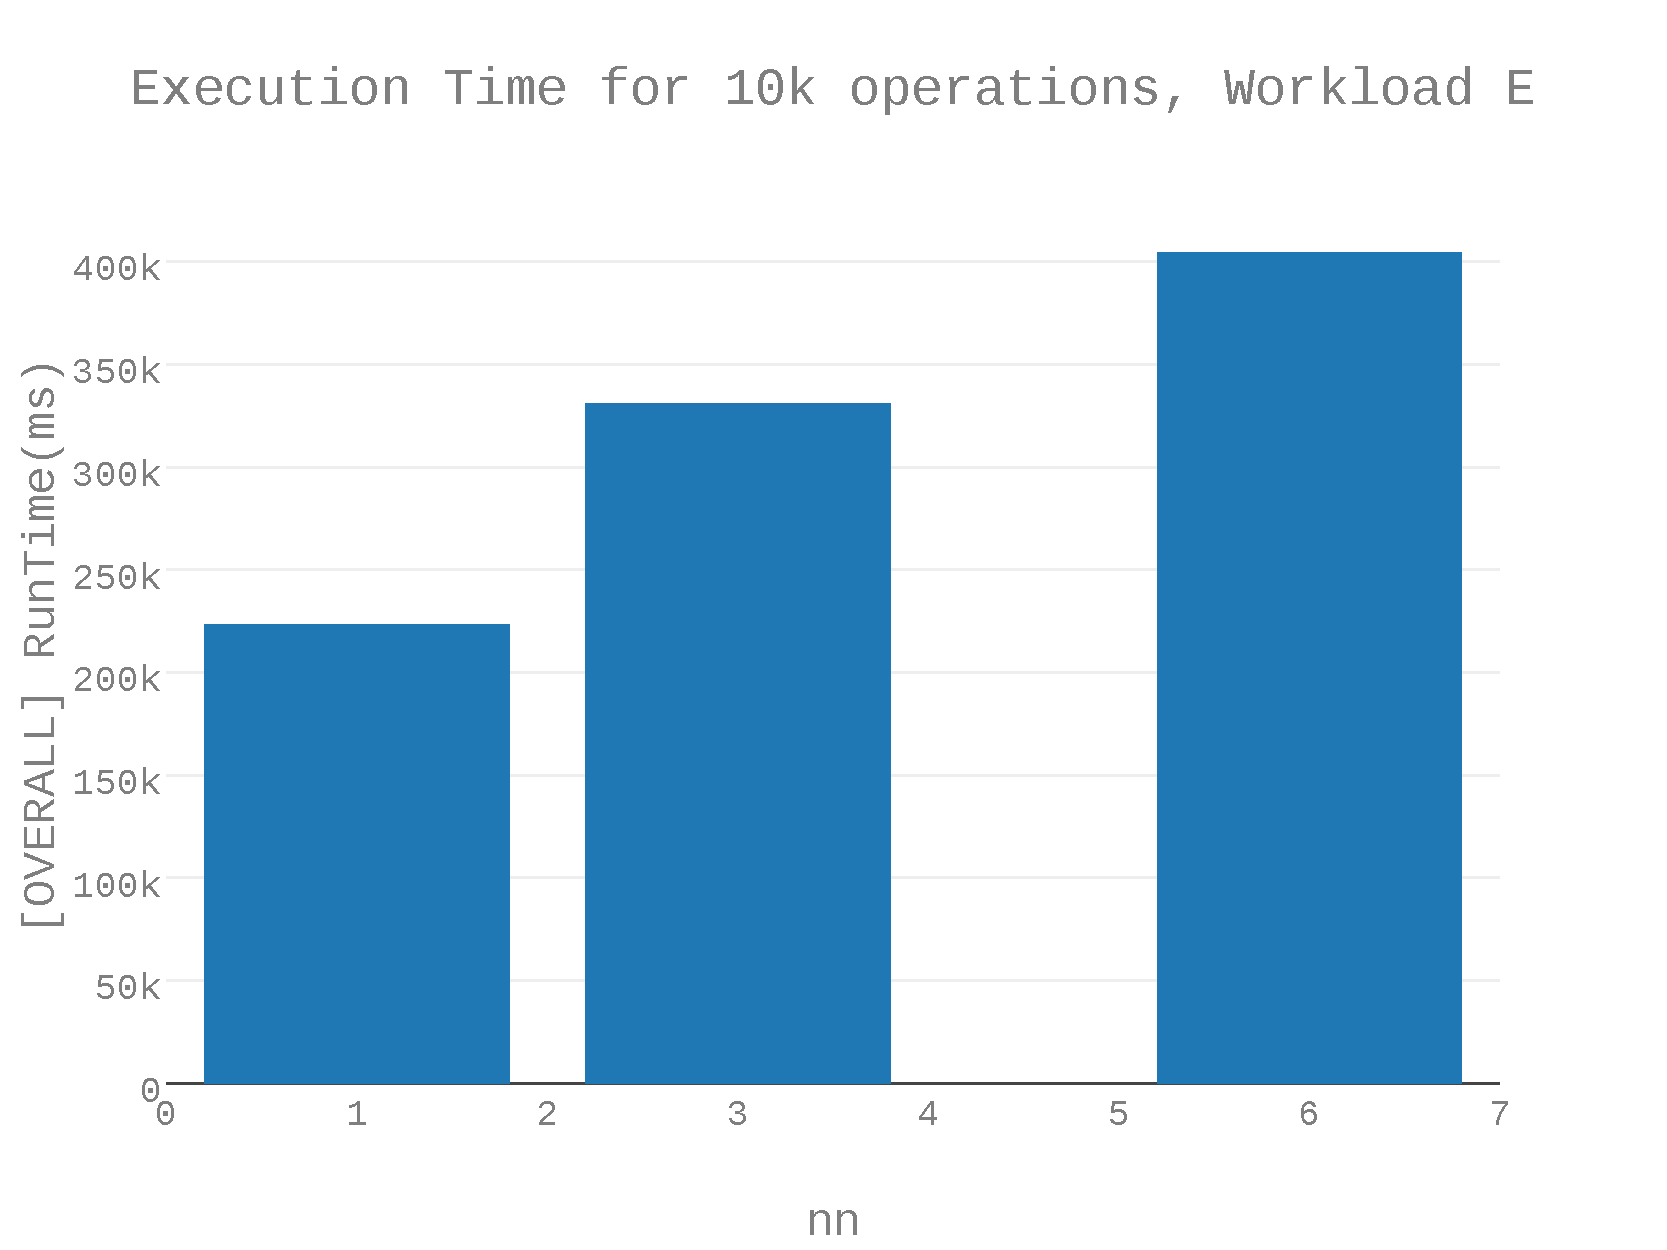
\includegraphics[width=3.5in]{Figures/figures-wle_fig1.pdf}

\caption{Cross Section of Results Imported from \cite{Abramova2014}.  This figure shows the execution time reported for 10,000 operations of Workload E over three given configurations: a network with only one (1) node, a network with 3 nodes, and a network with 6 nodes.}

\label{fig:wle_fig1}
\end{figure}

\section{Objective of This Set of Experiments}

The objective of this experiment is to characterize varying configurations for Cassandra.  This characterization will be in service of assessing the utility of Cassandra on the Raspberry Pi 2, which will in turn be an indicator toward the greater population of both distributed databases, archetype Cassandra, and hardware of archetype Raspberry Pi.

We aim to recreate results in \cite{Abramova2014} and then extend these experiments for a better characterization for \gls{iot}. In doing so, we answer the following research questions:
\begin{itemize}
\item Research Question 1: How much is the execution time for a given number of operations extended in the system under test using workload A (reads/updates)? 
\item Research Question 2: How much is the execution time for a given number of operations extended in the system under test using workload C (reads)?
\item Research Question 3: How much is the execution time for a given number of operations extended in the system under test using workload E (insert/scans)?
\item Research Question 4: And finally, how much is the execution time for a given number of operations extended in the system under test using custom workload I, the anticipated representative of in-situ distributed database \gls{iot} application?
\end{itemize}

To answer each of these questions, we aim for the following:
\begin{itemize}
\item Following the methodology, modified from \cite{Abramova2014}, observe and analyze the results of running the \gls{ycsb} for (at least) 1, 3 and 6 node networks for 2GB and a database size of 1 million records.
\item Extend the 2GB \gls{ram} virtual node: Vary the virtual machine's allotted \gls{ram} for similar \gls{iot} sizes of memory (512MB, 1GB, 4GB).  Observe and analyze for any effect.
\item Extend to Raspberry Pi 2 modules, which have 1GB of memory.  Observe any differences.
\item Extend to a wireless \gls{lan}.  Observe any differences.
\end{itemize}

\section{Expectations}

The results of these experiments are anticipated to be within reasonable bounds of previous work \cite{Abramova2014}.  The results are not, however, expected to provide enough data points to provide a utilitarian mathematical model.  Such a model is alluded to in future work.

\section{System Boundaries}

Virtual machine nodes were contained in a single laptop.  The wired \gls{lan} experiments were performed with all nodes and the associated router within about 3 meters of one another on a dedicated \gls{lan}.  Likewise, the wireless \gls{lan} experiments were performed with all nodes and the router within a radius of 3 meters on a dedicated and secured \gls{lan}.  The experiments were done in a residential, suburban area. The network was periodically monitored for unexpected hosts.  

\section{Experimental Limitations, Nuisance Factors, Known/Suspected Interactions}

The amount of interference on the \gls{ism} band could not be controlled.  It is left to the assumptions that any variation in interference was negligible between any two trials.

The laptop running the \gls{ycsb} may have been running other minor programs or other processes to a limited extent.  No experiments were done to determine if this would have a significant effect, and this was not strictly controlled.

\section{Coordination}

\subsection{Ethernet \gls{lan}}

No coordination was needed.  This network was physically isolated and no additional traffic was expected to interfere with it.

\subsection{Wireless \gls{lan}}

Because the scale and timing of this experiment was limited, there was no formal coordination needed.  However, because a larger experiment could possibly fill up one (or more) frequency channels, one must be courteous of the environment.  An extended test would not be appropriate in an uncontrolled environment.

\section{Treatments, Independent Variables}

The independent variables of interest are the node type and link type.  Node type is characterized by memory, or \gls{ram}, processor speed, and \gls{io} rates, and are represented by virtual nodes and the Raspberry Pi.

The link types are the internal nodes on the virtual machine network, Ethernet links, and wireless 802.11 links.

There are many other factors at work, but other factors, like workload, are only varied to give appropriate context to the variance in node type and link type. 

\section{Factors}

\subsection{Hard Disk Storage: \gls{sd} Card}

The manufacturer and model for each \gls{sd} card was kept constant for each node.  The details can be found in \ref{table:sd_card_specs}

\begin{table}
\begin{center}
 \begin{tabular}{||c c||} 
 \hline
 Specification & Value \\ [0.5ex] 
 \hline\hline
 Capacity & 16 GB \\ 
 \hline
 Read Speed & up to 90 MB/s \\
 \hline
 Write Speed & up to 40 MB/s \\ 
 \hline
 Video Speed & C10 U3 \\ [1ex] 
 \hline
\end{tabular}
\end{center}

\caption{Specifications for SD Cards \cite{SanDiskCard}}
\label{table:sd_card_specs}
\end{table}


\subsection{Database Size}

This work assumes that an in-situ storage application in the realm of \gls{iot} implies a small database, in this case represented by 1 million records, as opposed to 10 million or 100 million or more.  Although Abramova’s paper seems to imply there is feasibility for large database with many, many nodes given the right balance, this work focuses more on the initial impact to performance of introducing less-capable hardware in order to lighten costs or actual physical weight for an application that would see this as a benefit.

\subsection{Number of Operations Per Trial}

The results in \cite{Abramova2014} report an execution time after 10,000 operations, and the decision was made to keep this constant rather than vary the representative number of operations.  No explicit justification is given in \cite{Abramova2014} for the number 10,000, but it can be inferred that it lies somewhere between being too small to represent the population (1 or 2 operations would be too small), and a sample size too large, that which merited exchange with a smaller sample size that could achieve the same aim.  But, one can take a minor step further.

As a brief experiment, one can take a look at what it might look like to vary the sample size in a given trial, and how the execution time would vary over the sequence of trials.  The graph above shows this for two different configurations: 1GB and 4GB RAM on a virtual machine.  As expected, the execution time does reflect initial cache warm-up time, but then, more or less, reflects some sort of steady state, albeit oscillating performance.
It was also not made explicit whether or not the 10,000 operations represented one of many trials of 10,000 or represented a single and only trial.  For the purposes of exploring the data, this author chose to run 30 trials of 10,000 operations each.

\begin{figure}[h]
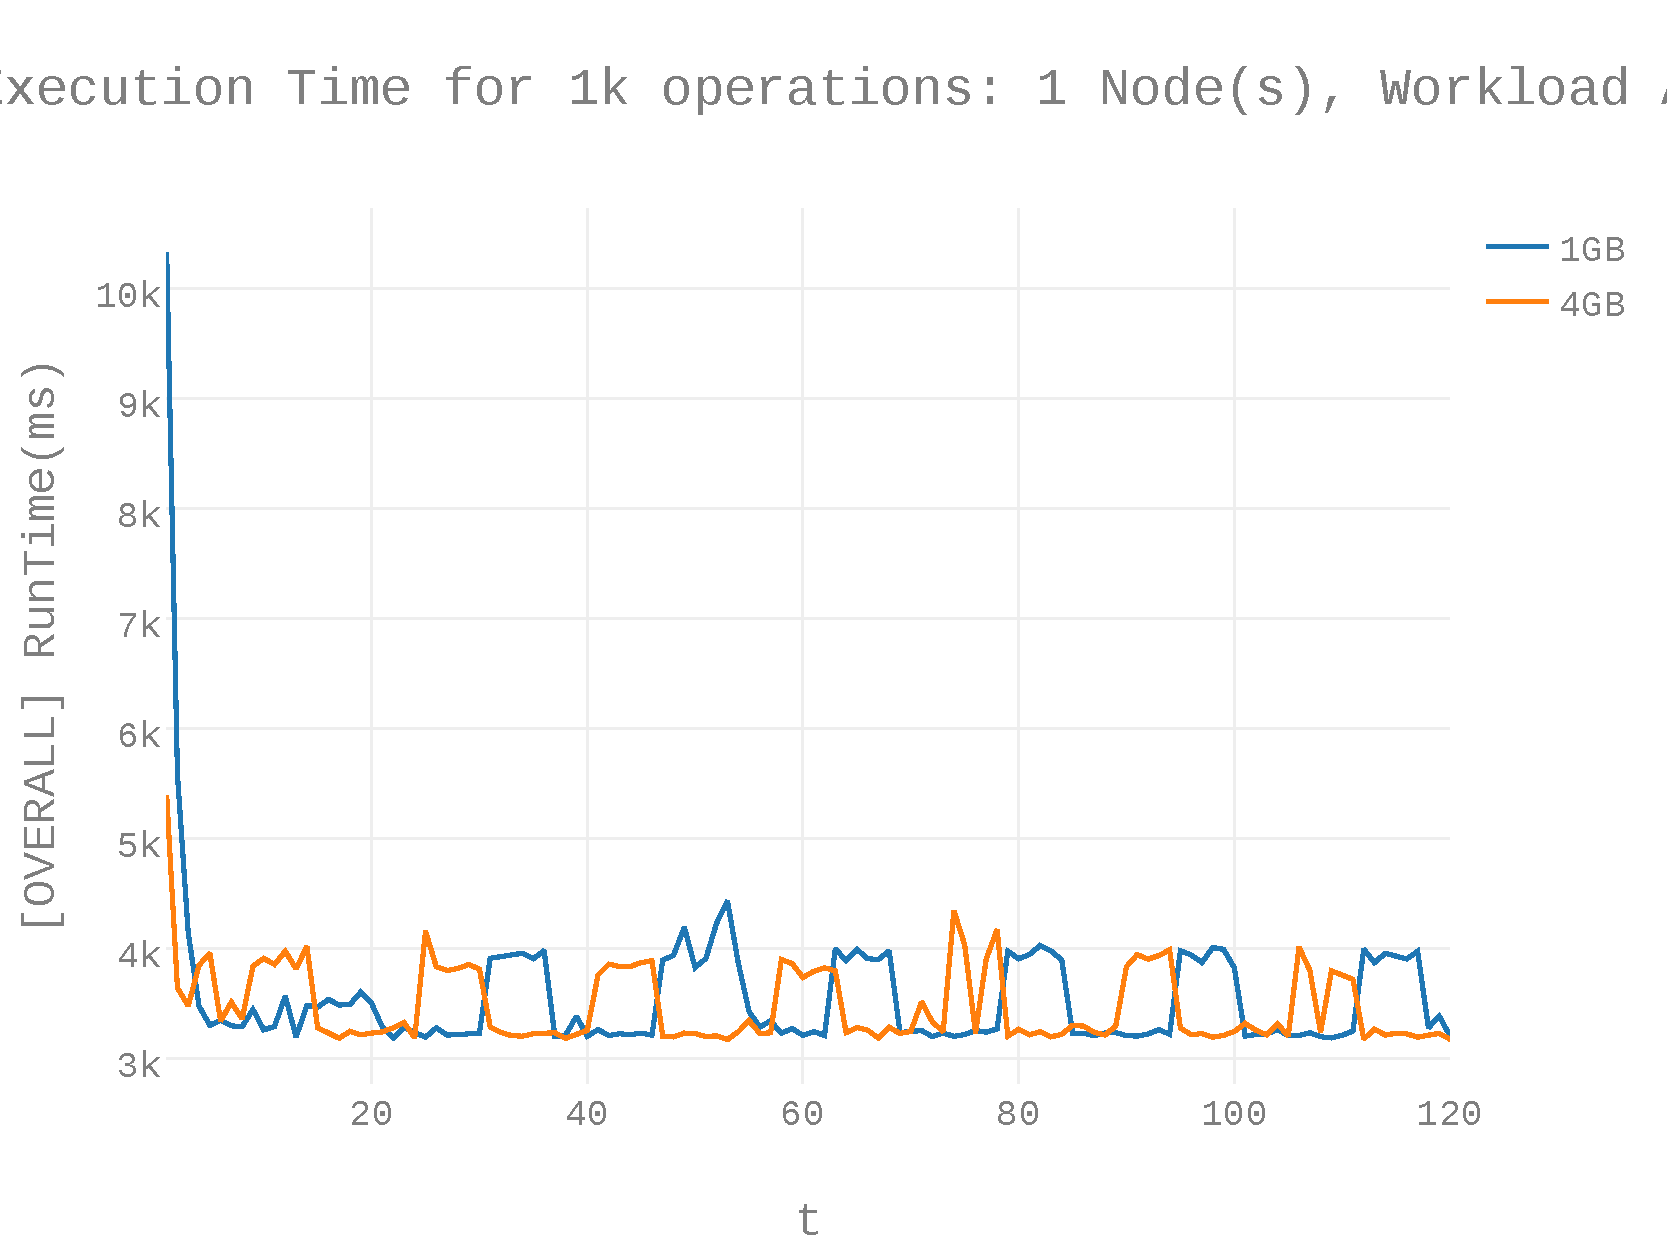
\includegraphics[width=3.5in]{Figures/figures-wla_fig2.pdf}

\caption{Two sample runs, adjusting the trials such that only 1000 operations of Workload A to a given trial.}

\label{fig:fig02}
\end{figure}

The oscillating behavior seen in trials 5 through 120 is distracting and risks inaccurate comparisons among configurations.  Although it is beyond the scope of this paper to determine the exact cause of this oscillation, one might consider that activities required for the operation of the database, such as compaction, the gossip protocol, and other operations compete with the reads and will contribute to continuous variation over time, and may affect performance measurements.  The reason for choosing 10,000 operations is not explicitly reported in \cite{Abramova2014}, but one may infer the reason is to integrate this variation to make better comparisons among configurations.  

\begin{figure}[h]
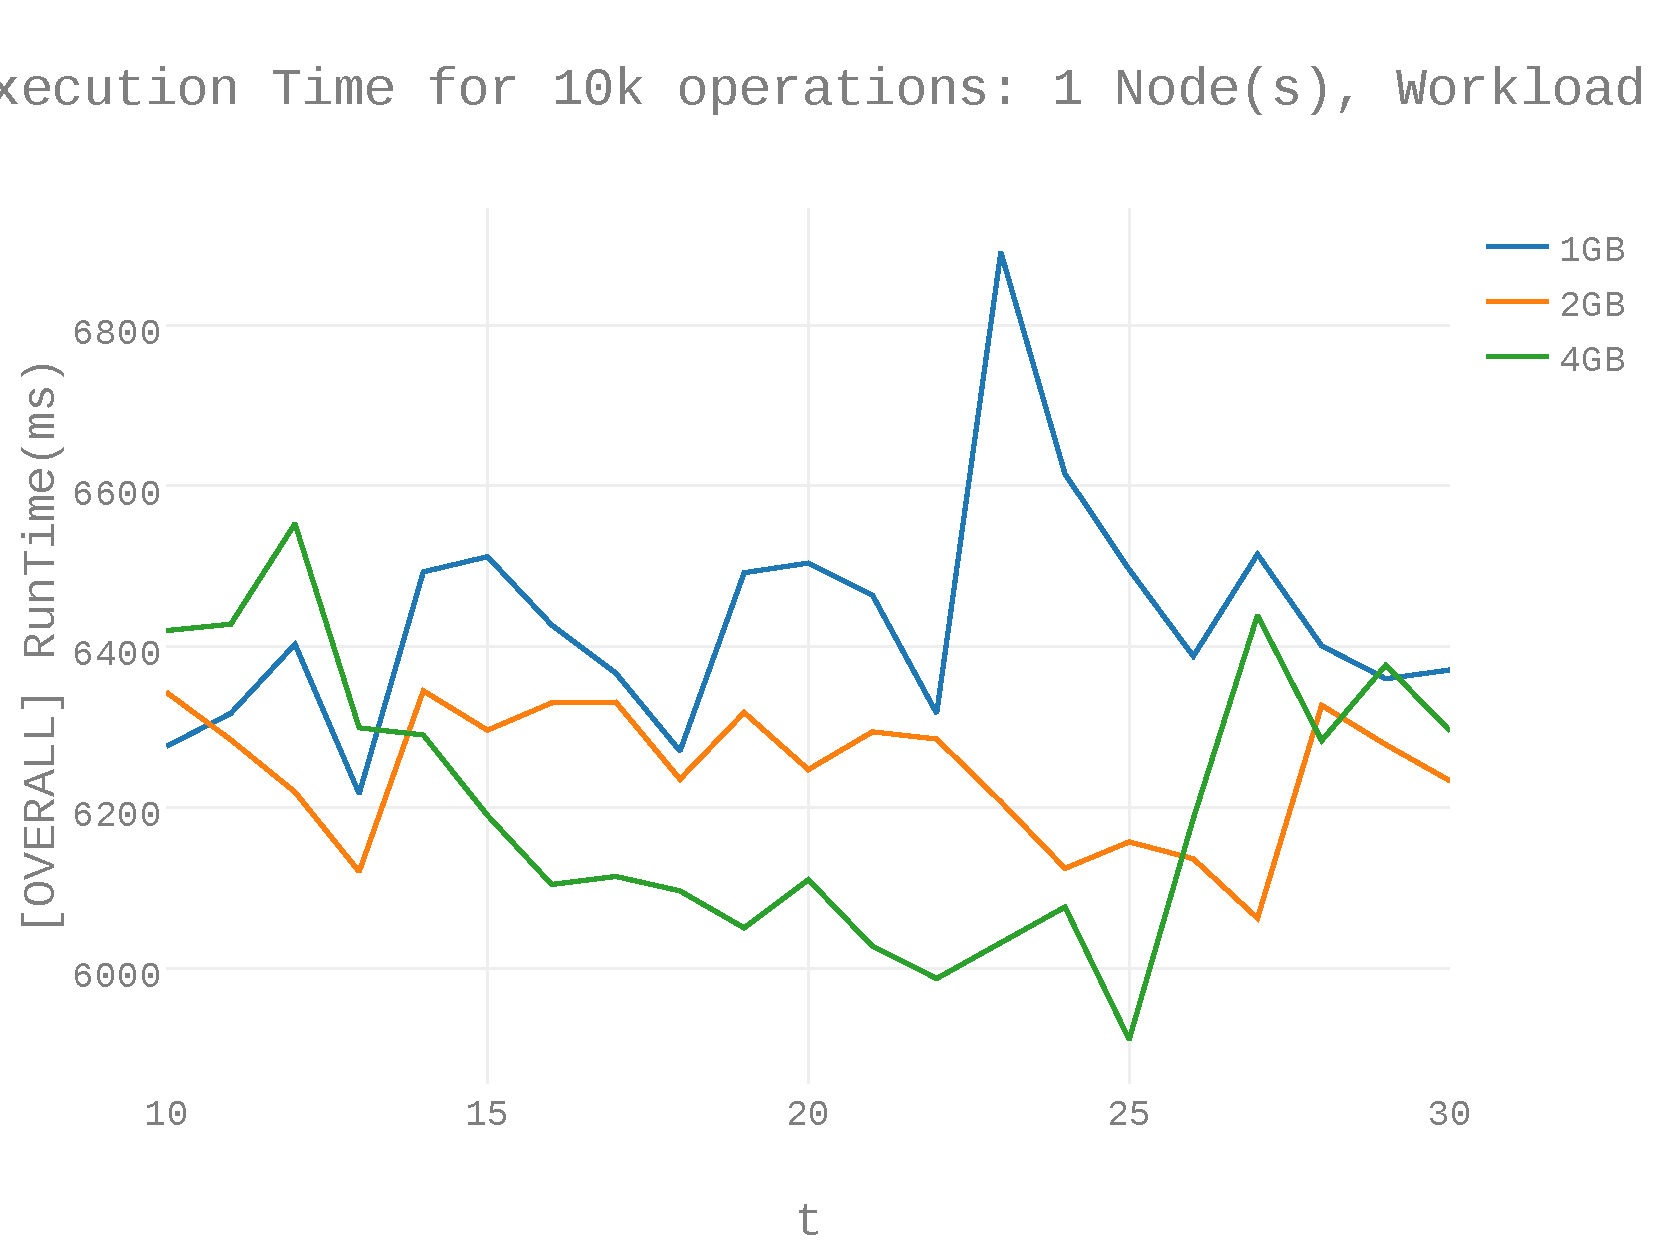
\includegraphics[width=3.5in]{Figures/figures-wla_fig3.pdf}

\caption{A series of trials for 1GB, 2GB, and 4GB \gls{ram} virtual machines.  The inset demonstrates that any pattern that could significantly distinguish one trial from another, such as the oscillation seen in \ref{fig:fig02} is integrated such that, after the cache warm-up period, the relative position of the trial does not predict the relative outcome.}

\label{fig:fig03}
\end{figure}

Contrast the 1k operation trials with the 10k operation trials depicted in \ref{fig:fig03}.  Here, at least with the naked eye, there is no oscillation, and most certainly not to the extent seen in the 1k trial case.  Whatever effected the oscillating behavior in the previous graph is integrated into the 10k trial case and is no longer a distraction to steady-state analysis, as each 10k operation trial soaks up, or rather integrates, the performance of quantity 10 1k operation trials.  Of course, more operations take longer to run, and thus the cost in testing time starts to curtail the value of integrating more trials.

\subsection{Workloads}

Just as in \cite{Abramova2014}, standard workloads A, C, and E were put to the test, while B, D, and F are saved for future work.  In addition, this paper introduces a custom workload, denoted I, to represent an \gls{iot} application, many inserts and few reads, a 99 percent to 1 percent ratio.

Standard workloads A, C, and E, from the \gls{ycsb} are summarized in Table \ref{table:std_workloads}.
\begin{table}
\begin{center}
 \begin{tabular}{||c c c c||} 
 \hline
 Workload & Read & Update & Scan \\ [0.5ex] 
 \hline\hline
 A & 0.5 & 0.5 & 0.0 \\ 
 \hline
 C & 1.0 & 0.0 & 0.0 \\
 \hline
 E & 0.0 & 0.0 & 1.0 \\ [1ex] 
 \hline
\end{tabular}
\end{center}

\caption{Standard \gls{ycsb} workloads used in this methodology.  Workload A consists of 50 percent reads and 50 percent updates.  Workload C consists of 100 percent reads.  Workload E consists of 100 percent scans.}
\label{table:std_workloads}
\end{table}

\begin{table}
\begin{center}
 \begin{tabular}{||c c c c c||} 
 \hline
 Workload & Read & Update & Scan & Insert \\ [0.5ex] 
 \hline\hline
 A & 0.50 & 0.50 & 0.00 & 0.00 \\ 
 \hline
 C & 1.00 & 0.00 & 0.00 & 0.00 \\
 \hline
 E & 0.00 & 0.00 & 1.00 & 0.00\\ 
 \hline
 I & 0.01 & 0.00 & 0.00 & 0.99 \\ [1ex] 
 \hline
\end{tabular}
\end{center}

\caption{Standard \gls{ycsb} workloads used in this methodology.  Workload A consists of 50 percent reads and 50 percent updates.  Workload C consists of 100 percent reads.  Workload E consists of 100 percent scans.  In addition, a custom workload I is summarized, which consists of 99 percent writes and 1 percent reads to represent \gls{iot}.}
\label{table:std_workloads_with_i}
\end{table}

In this experiment, we measure the total run time of a fixed number of operations of Workload A for various memory sizes. The choice of memory size is due to the expectations of \gls{iot} devices. The Raspberry Pi 2 and 3 have 1GB of memory and is our representative technology for \gls{iot}. The 4GB configuration can be considered be more representative of a low-end desktop, laptops, or virtual machine. The 2GB configuration is an intermediate stage that show an intermediate performance level and naturally, may represent the aim of future of \gls{iot} nodes. In addition, \cite{Abramova2014} used 2GB machines, which may help this work to be compared against existing work.

For this work, virtual nodes were created to match these characteristics to a reasonable extent.  Facing minimal propagation delay due to being connected on a nodal network, experiments with the virtual machines seek to place an upper limit on potential \gls{iot} performance expectations. Replicating the exact network in \cite{Abramova2014} is not absolutely necessarily, notwithstanding the details and materials available to do so are unavailable.

\subsection{Configuration of Cassandra}

Unless otherwise specified, the configuration of Cassandra, the keyspace, and the table within the keyspace are all held constant to their default values.  All three of these things can be configured hierarchically, and their configuration can affect the performance of Cassandra on a given load.  A skillful adjustment of these parameters can result in an optimized performance of Cassandra.

This paper aims to highlight the differences in varying hardware, and thus the exact configuration, despite that it might raise the absolute level of performance, is not expected to elevate the relative level of performance one would see shifting between, say a virtual node on a laptop and a Raspberry Pi module.

There are a few settings that had to be taken into account.  Denoted $commitlog\_total\_space\_in\_mb$, this will accumulate to an undesired level.  This was set to 512 MB in the Cassandra configuration file, cassandra.yaml.  (Changing this to 256 MB for the 512 \gls{ram} case did not correct the error mentioned above.)  Also, to prevent the accumulation of space, the setting $auto\_snapshot$ to false in configuration file cassandra.yaml.  Having $auto\_snapshot$ set to true automatically backs up, or saves a snapshot of, the data on Cassandra.  For a limited-capacity node, this is a luxury one cannot afford.

The configuration files can be found among the appendices.

\subsection{Threads in the \gls{ycsb}}

The number of threads was kept constant at 1, although by increasing the number of threads one could achieve greater throughput.  However, since it was desired to compare different calculations, the default was retained for all configurations.

It may be worth noting that for loads, this number was increased for practical reasons.  However, pure writes were not measured in these experiments, only the defined workloads A, C, E, and custom workload I.

\section{Assumptions}
\label{Assumptions}

Naturally, in order to perform the experiment and evaluate the results, some assumptions had to be made.
Investigation into any of these assumptions may be a lead into future work.

\begin{enumerate}

\item The benchmark represents the application, which assumes a simple schema.  In other words, Cassandra's performance is not particularly sensitive to the schema.

\item There is no active attacker or intrusion into the local area networks.  Both the local area networks are isolated.

\item There are no errors with the custom benchmark that would skew the results.  Any error is due to the fact that the system's limits have been reached.

\item There are no bugs in the benchmark that would skew the results.

\item Effects on the network due to distance are negligible.

\item This experiment assumes that nodes are homogeneous.  The basis for this assumption is that all nodes have been specified to the same model of Raspberry Pi 2.  The same make and model for the SD Cards have been used.  The image upon the SD Cards has been copied and only adjusted to account for specific, differentiated IP addresses.

\item This experiment assumes an uninterrupted power supply.  Power supply has no bearing on Cassandra’s performance on the hardware cluster, and is not measured nor accounted for in the model.

\item This experiment assumes an uninterrupted power supply.  Power is not measured nor accounted for in the model.  As long as the power has been turned on, it stays on, and fluctuations in voltage or any kind of imperfections in the power supply are negligible with respect to Cassandra's performance.

\item Although the ISM band is unregulated, this experiment assumes invariant interference from other emitters.  The experiment assumes an urban to suburban environment.  In other words, congestion that overwhelms Cassandra's performance can be assumed to be rare with respect to the population, and is ignored for the purposes of the experiment.

\item Another note on interference for the wireless configurations.  This experiment assumes invariant interference regardless of how much data is being written to the table in Cassandra. For the given pet application, collecting WiFi signals, the benchmark may be related to the amount of expected interference.  Probe requests can be indicative of WiFi traffic with which Cassandra might be competing, but this would require further investigation.  

\end{enumerate}

\section{Experimental Setup}

The experiments performed can be summarized in Table \ref{table:topologies}.
\begin{table}
\begin{center}
 \begin{tabular}{||c c c||} 
 \hline
 Communication (nm) & Platform (nt) & Assigned RAM \\ [0.5ex] 
 \hline\hline
 Nodal & Virtual Machine & 1 GB \\ 
 \hline
 Nodal & Virtual Machine & 2 GB \\
 \hline
 Nodal & Virtual Machine & 4 GB \\
 \hline
 Ethernet LAN & Raspberry Pi & 1 GB \\
 \hline
 802.11 LAN & Raspberry Pi & 1 GB \\
 \hline
\end{tabular}
\end{center}
\caption{This table summarizes each network topology that was explored in each research question.  The \gls{ram} was varied on the Virtual Machines.  It was not of interest to attempt to vary the \gls{ram} on the Raspberry Pi nodes.}
\label{table:topologies}
\end{table}



\subsection{Virtual Node Setup}

For this work, virtual nodes were created to match these characteristics to a reasonable extent.  Facing minimal propagation delay due to being connected on a nodal network, experiments with the virtual machines seek to place an upper limit on potential \gls{iot} performance expectations. Replicating the exact network in \cite{Abramova2014} is not absolutely necessarily, notwithstanding the details and materials available to do so are unavailable.

On a 64-bit 31.1GiB RAM laptop with Intel Core i7-4910MQ 2.90GHz 8-core central processing unit, six (6) identical virtual machines were created in software VirtualBox.  Each machine consisted of Ubuntu 64 bit machine was was allocated 8 GB of hard drive disk space.  The full details for these machines, reported by means of the lshw Linux command, are located among the appendices.  Also in VirtualBox, a host-only network entitled vboxnet0 was instantiated, to which all six machines were connected.

The \gls{ycsb} was installed and run on the host laptop.  PyCharm drove a terminal process, which in turn drove the \gls{ycsb} software.

To further paint the picture of the network setup, the \gls{ip} addresses are included in Table \ref{table:ip_addresses_vm}

\subsection{Ethernet \gls{lan} Setup}

The wiring of the Ethernet \gls{lan} is depicted in Figure \ref{fig:topology_for_ethernet_setup}.  Note that for the Ethernet set up, the wireless capability for the home router was switched OFF.

All nodes, including the laptop used to execute the \gls{ycsb}, were on the same network.  Their \gls{ip} addresses are listed in Table \ref{table:ip_addresses_rp}.

\begin{table}
\begin{center}
 \begin{tabular}{||c c c c||} 
 \hline
 Node & Host Name & IP Address & Model \\ [0.5ex] 
 \hline\hline
 Node 1 & raspberrypi0 & 192.168.1.100 & 2B \\ 
 \hline
 Node 2 & raspberrypi1 & 192.168.1.101 & 2B  \\
 \hline
 Node 3 & raspberrypi2 & 192.168.1.102 & 2B \\
 \hline
 Node 4 & raspberrypi3 & 192.168.1.103 & 2B \\
 \hline
 Node 5 & raspberrypi4 & 192.168.1.104 & 2B \\
 \hline
 Node 6 & raspberrypi9 & 192.168.1.109 & 3 \\
 \hline 
 Laptop & daniel-ThinkPad-W541 &192.168.1.200 & - \\
 \hline
\end{tabular}
\end{center}
\caption{This table describes the \gls{ip} addresses in order to paint a further detailed understanding of network set up.  The netmask is 255.255.255.0}
\label{table:ip_addresses_rp}
\end{table}

\begin{table}
\begin{center}
 \begin{tabular}{||c c c||} 
 \hline
 Node & Host Name & IP Address \\ [0.5ex] 
 \hline\hline
 Node 1 & c0 & 192.168.56.100 \\ 
 \hline
 Node 2 & c1 & 192.168.56.101  \\
 \hline
 Node 3 & c2 & 192.168.56.102 \\
 \hline
 Node 4 & c3 & 192.168.56.103 \\
 \hline
 Node 5 & c4 & 192.168.56.104 \\
 \hline
 Node 6 & c5 & 192.168.56.105 \\
 \hline 
 Laptop & daniel-ThinkPad-W541 & 192.168.56.200 \\
 \hline
\end{tabular}
\end{center}
\caption{This table describes the \gls{ip} addresses in order to paint a further detailed understanding of network set up.  The netmask is 255.255.255.0}
\label{table:ip_addresses_vm}
\end{table}

\begin{figure}[h]
\centering
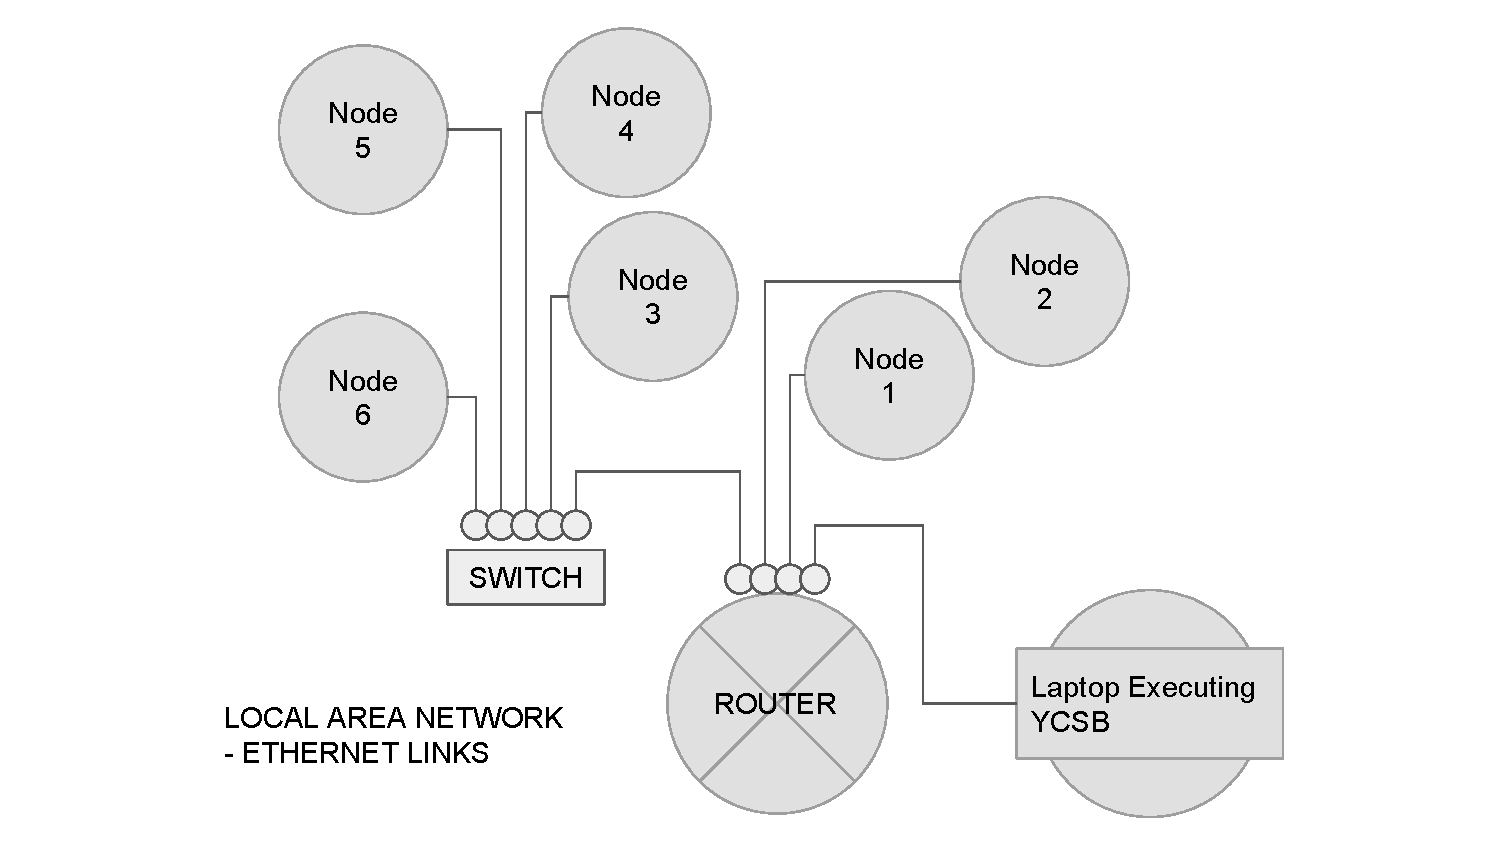
\includegraphics[width=7cm]{Figures/lan_eth.pdf}

\caption{Topology and Wiring for Ethernet Setup}

\label{fig:topology_for_ethernet_setup}
\end{figure}

\subsection{802.11 \gls{lan} Setup}

Table \ref{table:ip_addresses_rp_wireless} describes the local area network as the wireless the.  Note that for this setup, the Ethernet cables were physically unplugged.

To enable wireless links on the Raspberry Pi 2's, the Wi-Pi \gls{usb} module was utilized, with transmission speed capabilities listed at "11b – 1/2/5.5/11Mbps, 11g – 6/9/12/18/24/36/48/54Mbps, 11n – up to 150Mbps" \cite{RaspberryHut}.  The Raspberry Pi 3 model comes with its own built-in WiFi capabilities.

\begin{table}
\begin{center}
 \begin{tabular}{||c c c||} 
 \hline
 Node & Host Name & IP Address \\ [0.5ex] 
 \hline\hline
 Node 1 & raspberrypi0 & 192.168.1.130 \\ 
 \hline
 Node 2 & raspberrypi1 & 192.168.1.131  \\
 \hline
 Node 3 & raspberrypi2 & 192.168.1.132 \\
 \hline
 Node 4 & raspberrypi3 & 192.168.1.133 \\
 \hline
 Node 5 & raspberrypi4 & 192.168.1.134 \\
 \hline
 Node 6 & raspberrypi9 & 192.168.1.139 \\
 \hline 
 Laptop & daniel-ThinkPad-W541 &192.168.1.200 \\
 \hline
\end{tabular}
\end{center}
\caption{This table describes the \gls{ip} addresses in order to paint a further detailed understanding of network set up.  The netmask is 255.255.255.0}
\label{table:ip_addresses_rp_wireless}
\end{table}

\section{Execution}

The \gls{ycsb}, installed on the host laptop, is also run from the host laptop.  The \gls{ycsb} can be run from the terminal, but for convenience, a Python script was developed to drive a series terminal processes.

\section{Analysis}

For each experiment, the trials for each configuration will be reported as a summary of execution times for 10,000 operations.  All execution times will be reported in milliseconds.

\subsection{Response Variables}

The \gls{ycsb} reports a number of measured values, including operations per second and latency distribution (minimum, mean, 50 percentile or median, 75 percentile, 99 percentile, maximum).  The total execution time in milliseconds was chosen in order to keep the measured values true to the limits of the experiment.  Although operations per second and latency are more useful to know, since they are not confined to a fixed number of operations, the results in this paper are confined to 10,000 operations.  Although this paper aims to analyze results to reflect the steady state, this paper does not deny the possibility that variance in operations per second or variance in latency may result from variance in the number of operations (in this case, 10,000) per trial. 

\section{Cache Warm-Up Period and the Logic of Using the Median from This Point Forward}

Also, one can note in both Figure \ref{fig:fig02} and Figure \ref{fig:fig03}, that in the first five trials or so, one can observe the cache warm-up period.  This steep decline is expected due to the effect of the key cache, which is at it’s default setting: Cassandra sets the key cache to the either 5\% of the heap, or 100 MB, whichever is less.  In \cite{Abramova2014}, the key cache is reported to be at 100 MB.  The steady state operation is dependent on the keys requested, so for a workload like the YCSB, one would not expect a lot of variation.

Truncating the head of the trials, trials 1 though 9, the cache effect is no longer depicted, rendering an expectation of steady-state performance after cache warm-up.  This closer look indicates that varying \gls{ram} makes no significant difference in Cassandra’s performance.  This indicates that for the Raspberry Pi, and \gls{iot} devices in general, once a minimum threshold is reached in \gls{ram}, there are diminishing, if any, returns on performance for the potential inclusion of greater amounts of \gls{ram} on a piece of hardware. 

Taking the issues of oscillating behavior and cache warm-up period into account, we can remove them to find a stable viewing window into the behavior of the Cassandra database, as depicted in Figure \ref{fig:fig03}. Figure 4 shows the desired observation of the behavior in question for 1GB, 2GB ad 4GB memory sizes. We use this data to recreate Abramova’s work and extend it for other memory sizes.

Truncating the head of the trials, trials 1 though 9, the cache effect is no longer depicted, rendering an expectation of steady-state performance after cache warm-up.  This closer looks indicates that varying RAM makes no significant difference in Cassandra’s performance.  This indicates that for the Raspberry Pi, and IoT devices in general, once a minimum threshold is reached in RAM, there are diminishing, if any, returns on performance for the potential inclusion of greater amounts of RAM on a piece of hardware. 
This is the logic behind using the median to summarize the execution times.  The explanation here is the basis for the assumption that the median is a relevant summary statistic.  Of course, this is expected to hold true as long as there are at least 5 ‘steady-state’ data points to make up for the cache warm-up.

Another important observation here, is that once the cache effect is cropped out, there is no correlation between trials and the performance measurement.  This further supports that 10,000 operations, minus cache effect, does represent a steady state that is likely to extend beyond 10,000 operations.

This paper will then, for each workload, explore and compare the different network configurations, gauging the various conditional penalties that incur.  This paper will also gauge how Cassandra reacts having 1, 2, up through 6 nodes operating.  

%\chapter{Results}

\section{Results - Research Question 1}

This section presents the results of running \gls{ycsb}'s Workload A.

\section{Comparing Existing Work}

\begin{figure}[h]

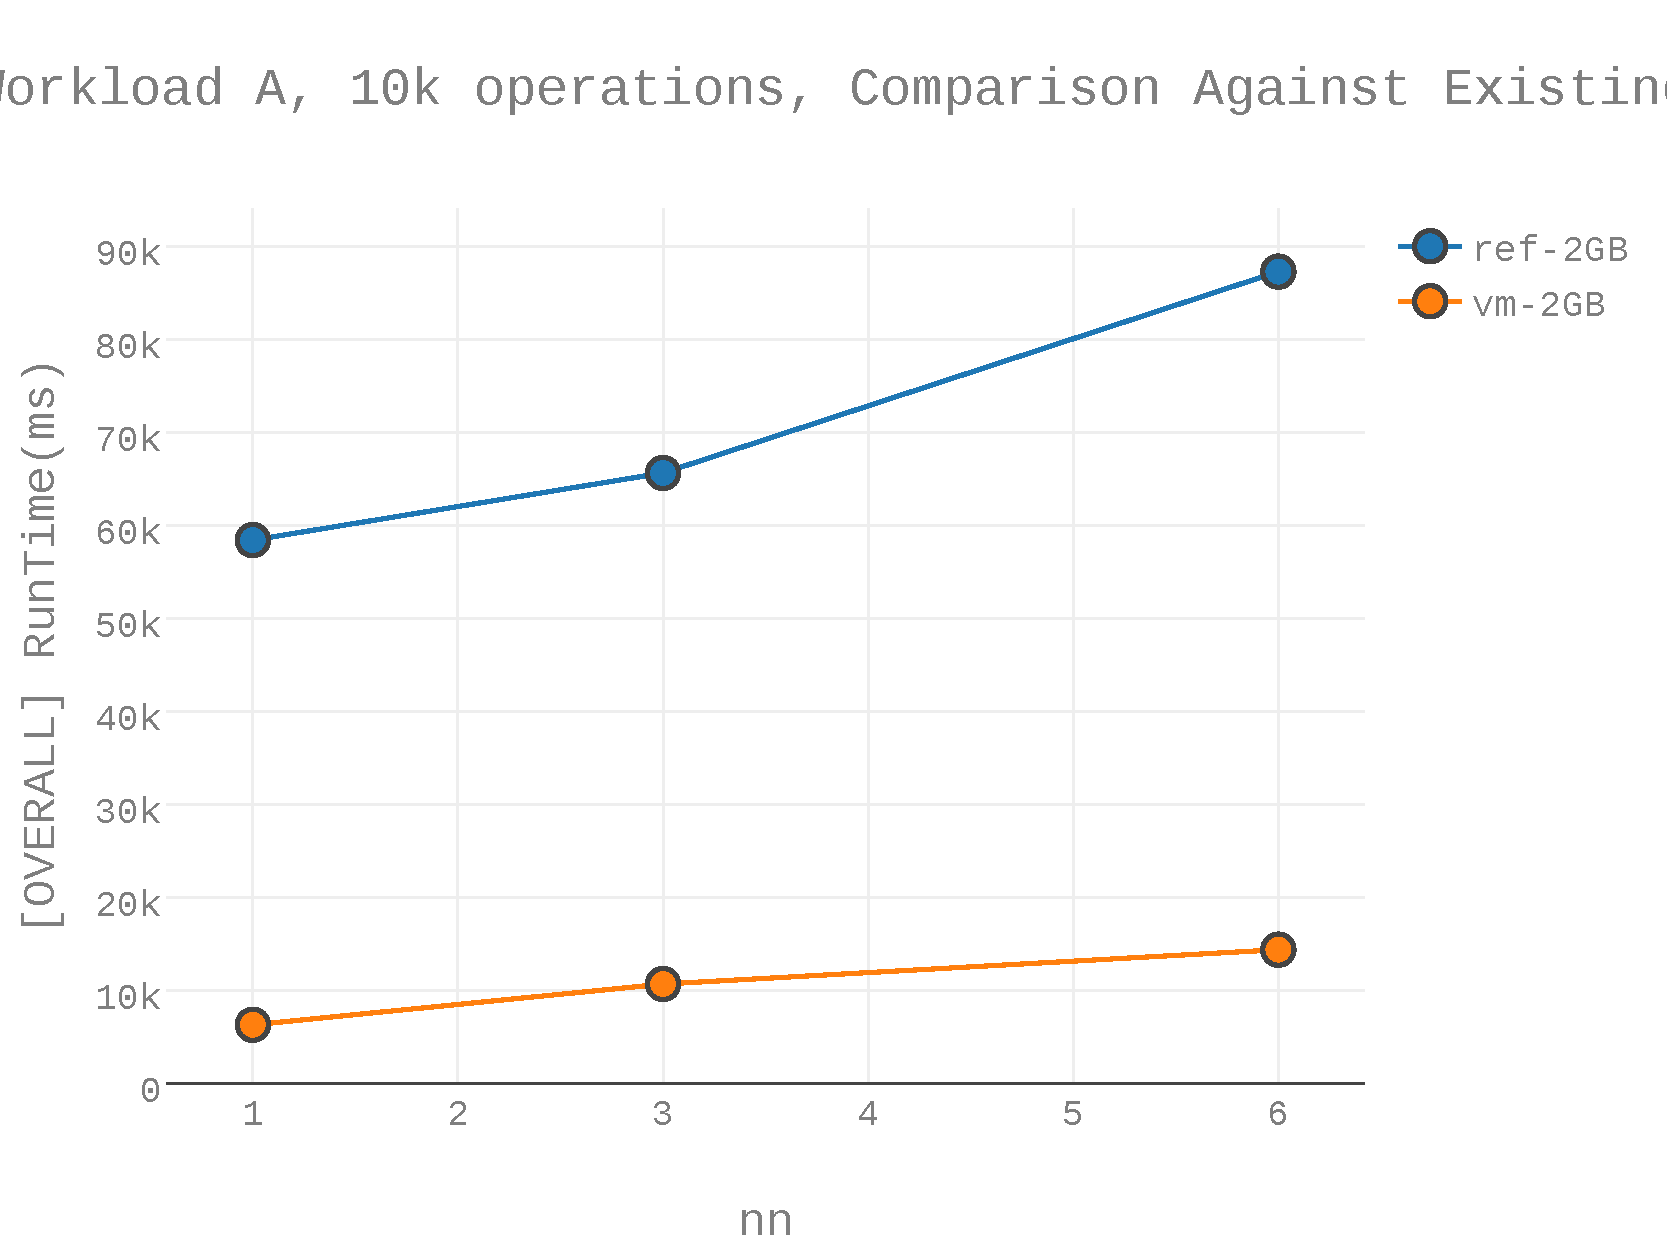
\includegraphics[width=6in]{Figures/figures-wla_fig5.pdf}

\caption{Comparing the results in \cite{Abramova2014} with the median value of the virtual machine assigned 2GB of \gls{ram}.  Note that the virtual machines were on a nodal network (minimal propagation delay) while the the links in \cite{Abramova2014} were unspecified.}

\label{fig:figures-wla_fig5}
\end{figure}

The summary for the 2GB-\gls{ram} virtual node are in Tables \ref{table:summary_statistics_for_1_config}, \ref{table:summary_statistics_for_3_config}, and \ref{table:summary_statistics_for_6_config} under column 'ram2GB'.    Figure \ref{fig:figures-wla_fig5} compares the results from \cite{Abramova2014} and the median execution times on a virtual machine environment for 1, 3, and 6 node configurations.  One can see a stark contrast between the execution times.

The most significant controlled difference between these two setups is the network.  The network in \cite{Abramova2014} is not specified, but generally a 'cluster' implies some kind of Ethernet configuration.  In a sense, this gives some insight into what kind of penalty one pays for switching from an ideal network to a physical one.

For the cluster sizes queried for this graph, both the virtual machine environment and the analagous workload done in \cite{Abramova2014} seem to positively correlate with cluster size.  This seems to indicate that, to a limited extent, the operations needed to ensure replication on multiple nodes overwhelm any advantage that dividing such operations among nodes.

One would expect, given that once this is extended to the Raspberry Pi modules, implying a physical network connection (Ethernet) and a 900 MHz processor compared to the 2.90 GHz processor used by the virtual machines, the performance would be represented by significantly longer execution time than that of the virtual nodes, possibly execution time comparable to the results in \cite{Abramova2014}.

Facing minimal propagation delay due to being connected on a nodal network and the same computing power as a laptop, in this work, results from the virtual machines seek to illustrate an asymptote on potential \gls{iot} performance expectations.

\section{Testing various memory sizes}

We now discuss testing and performance for memory sizes ranging from 512MB to 4GB.

\subsection{Minimum capability - 512MB}

This author reached a limit when attempting to examine operation with 512 MB of \gls{ram}.  Upon executing Cassandra, the program reported a deficiency in memory in order to operate.  This indicates that Cassandra has a minimum \gls{ram} capability to operate, although it is out of scope of this work to determine what parameters describe that limit.  

This author was not able to find an explicit hardware requirement for Cassandra, although in \cite{CassandraHardwareWiki}, a recommendation of 4GB RAM can be found.  However, the work in \cite{Abramova2014} shows that 2GB RAM is enough to run Cassandra.  This seems to suggest that through the right configurations of Cassandra, or Java upon which Cassandra runs, Cassandra might be able to work on platforms that have less RAM available.  With respect to this work, though not every configuration option was exhausted, and this may be an avenue for future work.    

\subsection{Experimental Testing for Memory in the 1GB – 4GB Range}

This section describes the results of running the \gls{ycsb} on virtual node networks as described in the methodology.  The summary of execution times are reported in Tables \ref{table:summary_statistics_for_1_config}, \ref{table:summary_statistics_for_3_config}, and \ref{table:summary_statistics_for_6_config}.  For each table, the summary statistics are listed for each amount of memory.

\subsubsection{Inspection of Results}

It is best to start with a visual inspection of the data represented in Figure \ref{fig:figures-wla_fig4}.  Generally with a greater amount of \gls{ram}, one might expect a correlation of fewer problems with memory overloads, or a lower frequency of compaction. However, inspection of each cluster size does not seem to indicate a correlation between memory and performance.

\begin{figure}[h]
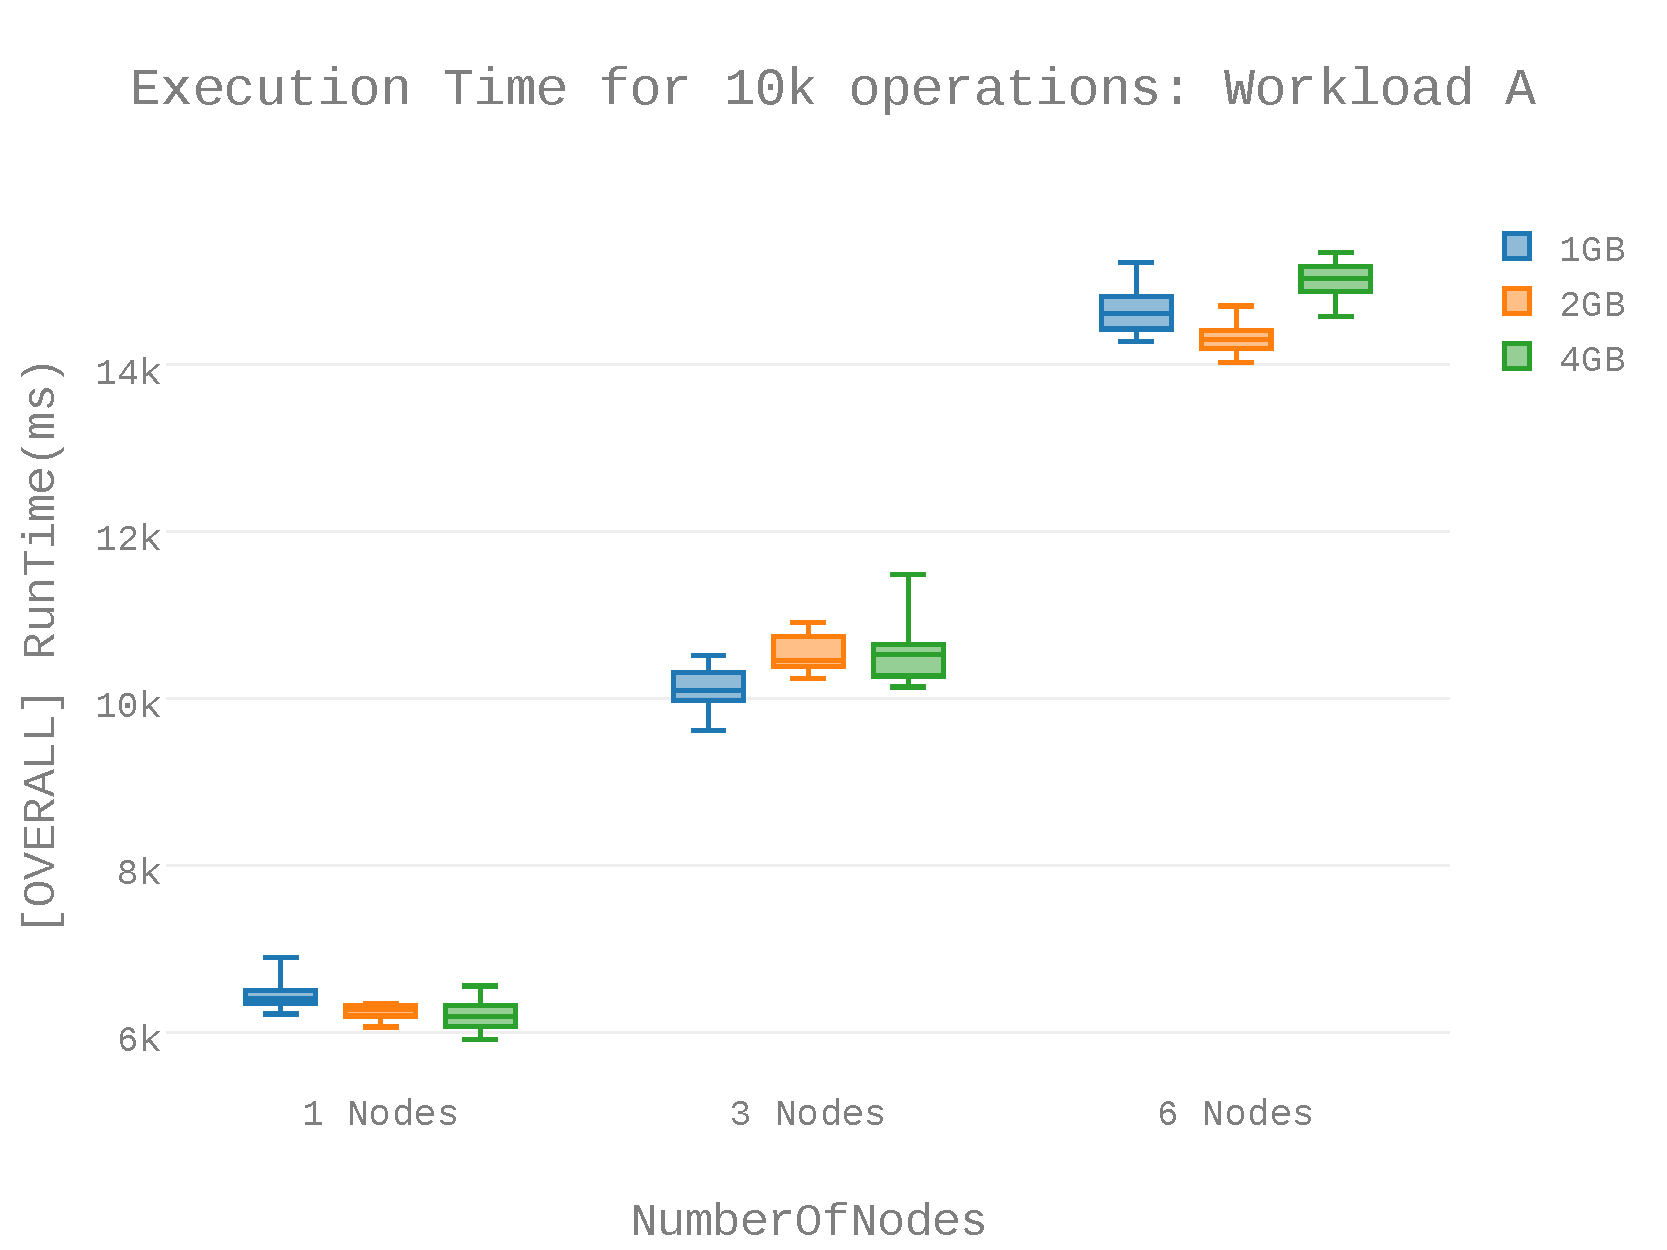
\includegraphics[width=3.5in]{Figures/figures-wla_fig4.pdf}

\caption{Execution time for virtual machines with 1GB, 2GB, and 4GB of \gls{ram}.  The first 9 trials have been removed in order to filter out the trials representing the cache effect and thus represent the steady state.}

\label{fig:figures-wla_fig4}
\end{figure}

\begin{table}
\begin{tabular}{lrrr}
\toprule
 index &  ram1GB &  ram2GB &  ram4GB \\
\midrule
 count &      21 &      21 &      21 \\
  mean & 6433.14 & 6246.24 & 6203.14 \\
   std & 144.084 & 84.0255 & 174.375 \\
   min &    6217 &    6062 &    5911 \\
   25\% &    6360 &    6207 &    6076 \\
   50\% &    6403 &    6278 &    6186 \\
   75\% &    6496 &    6318 &    6299 \\
   max &    6891 &    6345 &    6553 \\
 range &     674 &     283 &     642 \\
\bottomrule
\end{tabular}
\caption{Summary Statistics for 1-Node Configuration. All values represented fall between 5911.0 ms and 6891.0 ms, or rather within a span of 980.0 ms.}
\label{table:summary_statistics_for_1_config}
\end{table}

\begin{table}
\begin{tabular}{lrrr}
\toprule
 index &  ram1GB &  ram2GB &  ram4GB \\
\midrule
 count &      21 &      21 &      21 \\
  mean & 10127.9 & 10548.1 & 10549.1 \\
   std & 229.485 &  221.21 & 336.981 \\
   min &    9617 &   10235 &   10137 \\
   25\% &    9973 &   10382 &   10275 \\
   50\% &   10100 &   10456 &   10525 \\
   75\% &   10302 &   10735 &   10640 \\
   max &   10517 &   10910 &   11485 \\
 range &     900 &     675 &    1348 \\
\bottomrule
\end{tabular}
\caption{Summary Statistics for 3-Node Configuration. All values represented fall between 9617.0 ms and 11485.0 ms, or rather within a span of 1868.0 ms.}
\label{table:summary_statistics_for_3_config}
\end{table}

\begin{table}
\begin{tabular}{lrrr}
\toprule
 index &  ram1GB &  ram2GB &  ram4GB \\
\midrule
 count &      21 &      21 &      21 \\
  mean & 14659.3 & 14300.5 &   15000 \\
   std & 266.999 & 166.709 & 216.828 \\
   min &   14277 &   14030 &   14583 \\
   25\% &   14432 &   14200 &   14876 \\
   50\% &   14613 &   14298 &   15035 \\
   75\% &   14802 &   14407 &   15177 \\
   max &   15229 &   14705 &   15351 \\
 range &     952 &     675 &     768 \\
\bottomrule
\end{tabular}
\caption{Summary Statistics for 6-Node Configuration. All values represented fall between 14030.0 ms and 15351.0 ms, or rather within a span of 1321.0 ms.}
\label{table:summary_statistics_for_6_config}
\end{table}

\subsubsection{Absolute Ranges}

While Figure \ref{fig:figures-wla_fig4} gives a general sense of what the results look like, the actual summary statistics can be examined in Tables \ref{table:summary_statistics_for_1_config}, \ref{table:summary_statistics_for_3_config}, and \ref{table:summary_statistics_for_6_config}. After filtering out the first nine trials, the results for running 10,000 operations is displayed in Tables \ref{table:summary_statistics_for_1_config}, \ref{table:summary_statistics_for_3_config}, and \ref{table:summary_statistics_for_6_config}.  For each configuration, varying the \gls{ram} of the virtual machine resulted in execution times that fell within 2 seconds of each other.

\subsubsection{\gls{anova}}

A one-way \gls{anova} was performed with the filtered data, and the \gls{anova} summary tables can be seen in Tables \ref{ram_variance_analysis_workload_a_1_node}, \ref{ram_variance_analysis_workload_a_3_node}, and \ref{ram_variance_analysis_workload_a_6_node} for the 1, 3, and 6 node cases respectively.  For each case, the  p-value is much, much less than 0.05, and thus it can be said that one can be 95\% confident in the decision to fail to reject the null hypothesis that the means are equal.

\begin{table}
\begin{tabular}{lrrrrr}
\toprule
         Source &      SS &  df &      MS &   F &       p \\
\midrule
 between groups & 6.3e+05 &   2 & 3.1e+05 &  16 & 2.4e-06 \\
  within groups & 1.2e+06 &  60 & 1.9e+04 & nan &     nan \\
          total & 1.8e+06 &  62 &     nan & nan &     nan \\
\bottomrule
\end{tabular}
\caption{ANOVA Summary Table for Workload A, 1 Node}
\label{ram_variance_analysis_workload_a_1_node}
\end{table}

\begin{table}
\begin{tabular}{lrrrrr}
\toprule
         Source &      SS &  df &      MS &   F &       p \\
\midrule
 between groups & 2.5e+06 &   2 & 1.2e+06 &  17 & 1.2e-06 \\
  within groups & 4.3e+06 &  60 & 7.2e+04 & nan &     nan \\
          total & 6.8e+06 &  62 &     nan & nan &     nan \\
\bottomrule
\end{tabular}
\caption{ANOVA Summary Table for Workload A, 3 Node}
\label{ram_variance_analysis_workload_a_3_node}
\end{table}

\begin{table}
\begin{tabular}{lrrrrr}
\toprule
         Source &      SS &  df &      MS &   F &     p \\
\midrule
 between groups & 5.1e+06 &   2 & 2.6e+06 &  53 & 6e-14 \\
  within groups & 2.9e+06 &  60 & 4.9e+04 & nan &   nan \\
          total & 8.1e+06 &  62 &     nan & nan &   nan \\
\bottomrule
\end{tabular}
\caption{ANOVA Summary Table for Workload A, 6 Node}
\label{ram_variance_analysis_workload_a_6_node}
\end{table}

Examining the effects of variance in the amount of \gls{ram} allocated the virtual machines does not seem to have a notable impact on performance.  This indicates that, any observed limitation on the Raspberry Pis’ performance is not limited by \gls{ram}, but something else, and that varying \gls{ram} in future tests will not yield significant results.

% Insert something about statistical significance

\section{Implementation on Raspberry Pi}

In a similar fashion, the tests were run on the Raspberry Pi to observe performance.  The spread of each of the tests can be seen in Figure \ref{fig:wla_fig10} and Table \ref{table:wired-results}.  The results, next to one trend for the virtual machines, can be seen in Figure \ref{fig:fig06}. 

\begin{figure}[h]
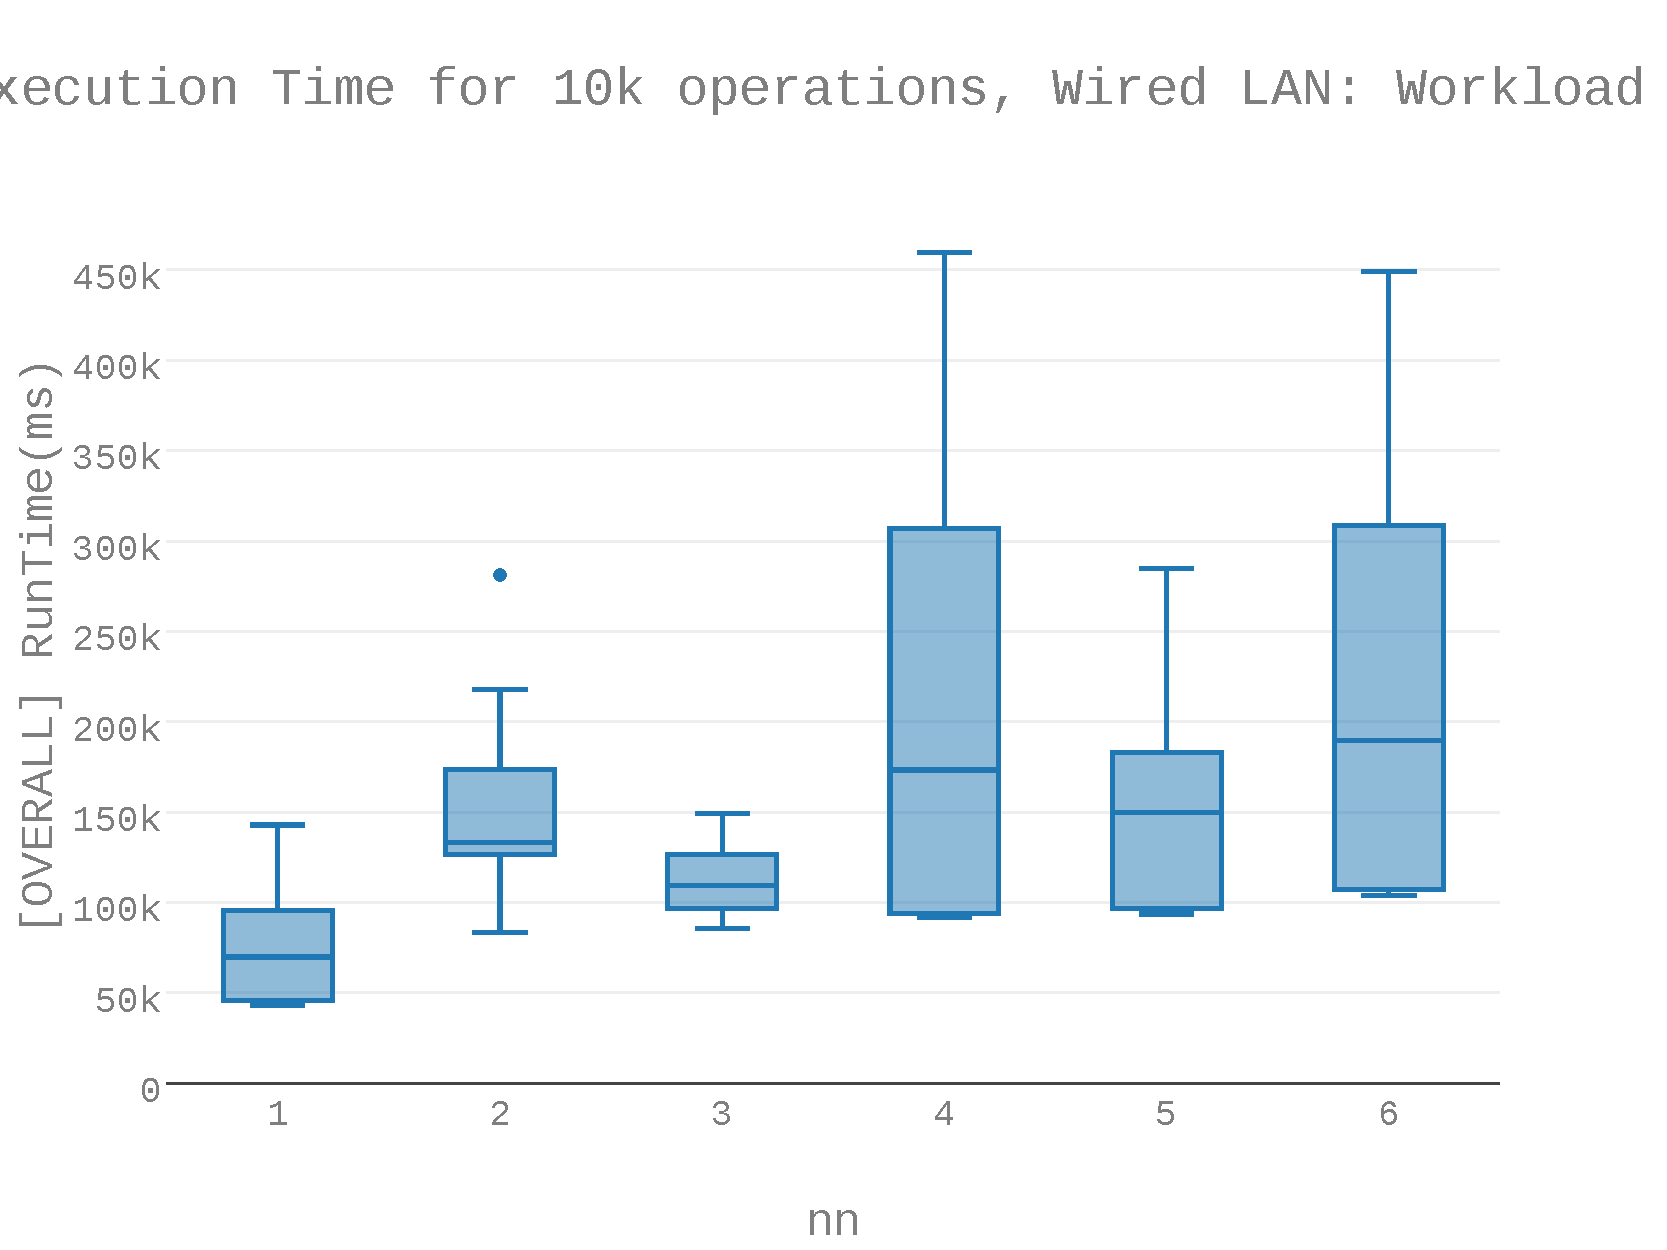
\includegraphics[width=3.5in]{Figures/figures-wla_fig10.pdf}

\caption{Box plot representing the results of the workload applied to wired local area network on the Raspberry Pi platform.}

\label{fig:wla_fig10}
\end{figure}

\begin{figure}[h]
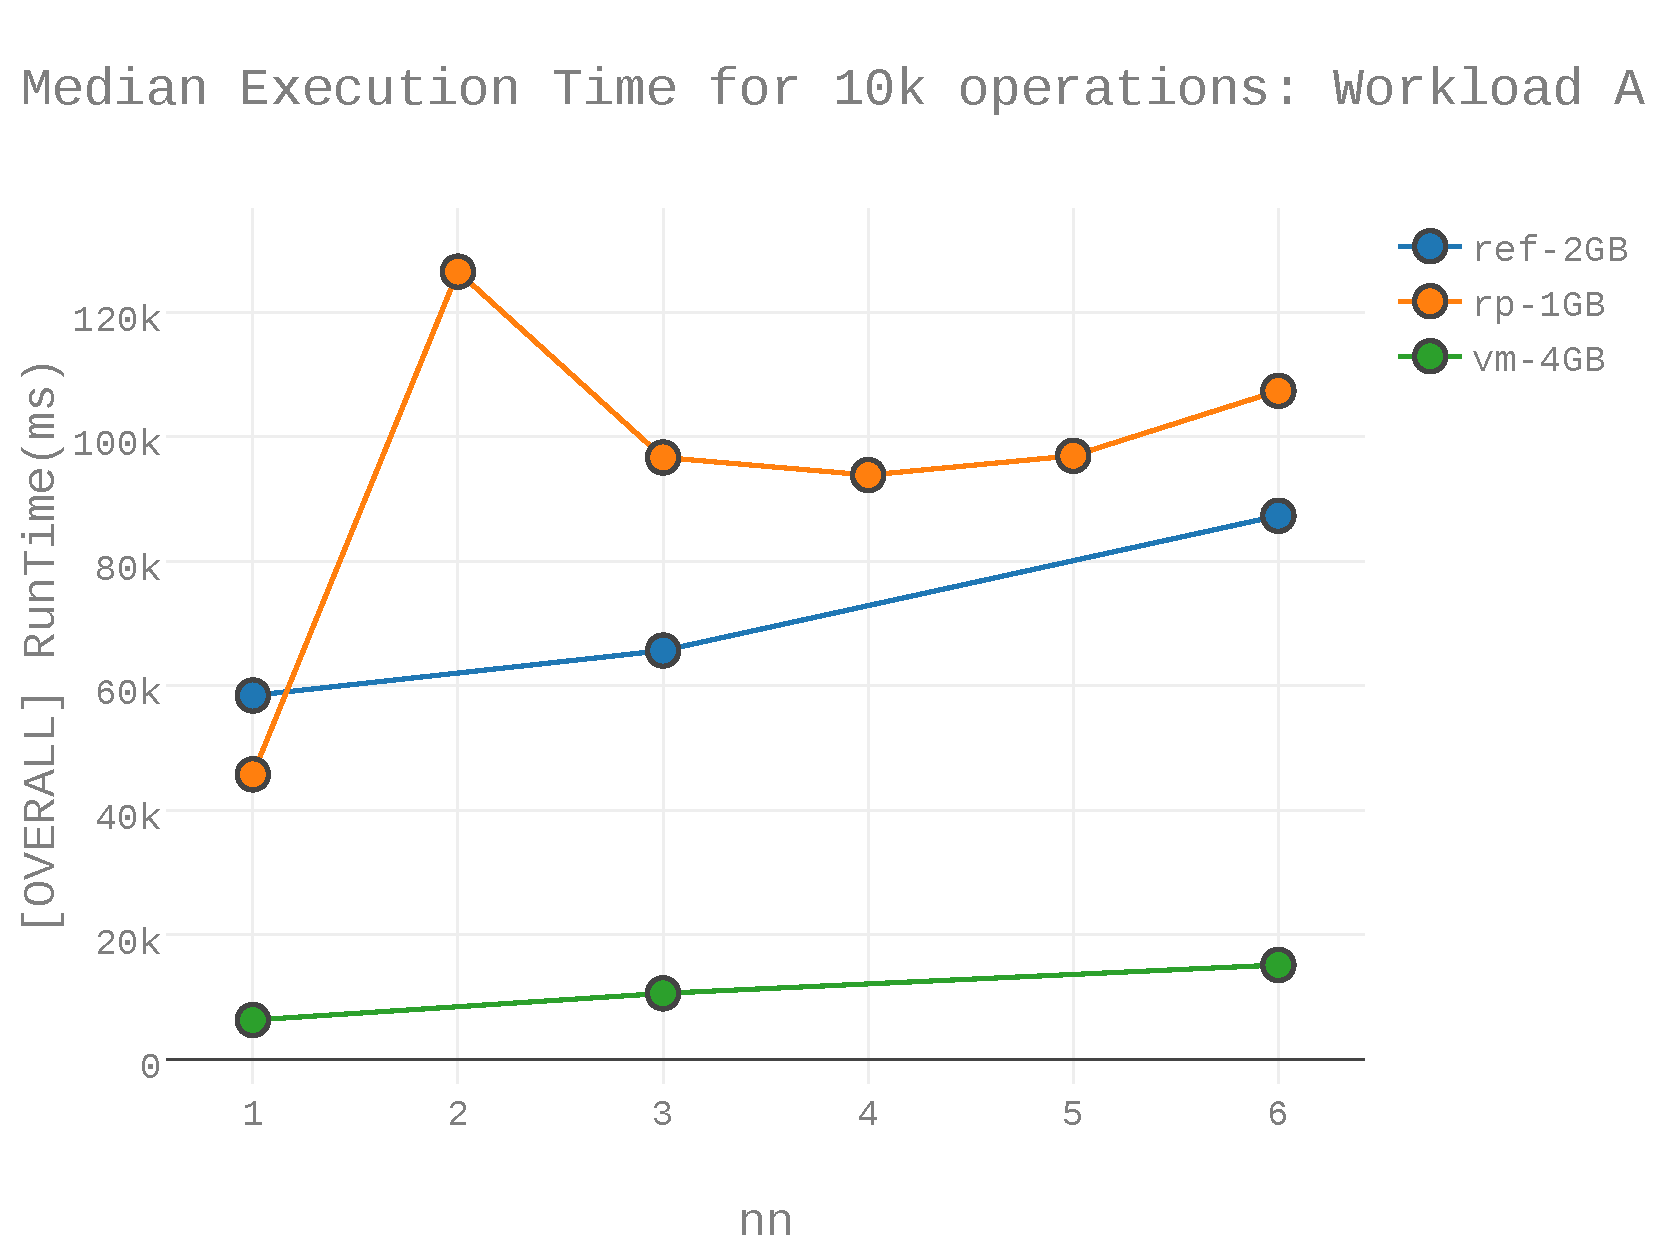
\includegraphics[width=3.5in]{Figures/figures-wla_fig6.pdf}

\caption{Comparison between the Raspberry Pi nodes (rp-1GB), the results reported in \cite{Abramova2014} (ref-2GB), and the virtual nodes with 4GB available \gls{ram} (vm-4GB).}

\label{fig:fig06}
\end{figure}

\begin{table}
\begin{tabular}{lrrr}
\toprule
 index &       1 &       3 &       6 \\
\midrule
 count &      21 &      21 &      21 \\
  mean & 4.6e+04 & 9.7e+04 & 1.1e+05 \\
   std & 1.1e+03 & 1.6e+03 & 1.8e+03 \\
   min & 4.3e+04 & 9.4e+04 &   1e+05 \\
   25\% & 4.5e+04 & 9.6e+04 & 1.1e+05 \\
   50\% & 4.6e+04 & 9.7e+04 & 1.1e+05 \\
   75\% & 4.6e+04 & 9.8e+04 & 1.1e+05 \\
   max & 4.8e+04 &   1e+05 & 1.1e+05 \\
 range & 4.9e+03 & 6.8e+03 & 7.3e+03 \\
\bottomrule
\end{tabular}
\caption{Summary for Raspberry Pi wired local area network}
\label{table:wired-results}
\end{table}

As can be seen from Figure \ref{fig:fig06}, the Raspberry Pi configuration takes considerably more execution time than the virtual machine analogy, which is probably due to the physical nature of the Ethernet connections (propagation delay) and the I/O limitations of the Raspberry Pi hardware.  However, its seemingly similar performance to the reference in \cite{Abramova2014} suggests the \gls{io} for the \gls{sd} Card follows a predictable pattern, and actually seems to outperform the node in \cite{Abramova2014} in the degenerate 1-node case.

For this paragraph, consider the results from \cite{Abramova2014} as the reference.  For a node network of 1, the experimental values fell between 43260.0 ms and 48123.0 ms, inclusive, and all values fell within 15170.0 ms of the reference value of 58430 ms.  For a node network of 3, the experimental values fell between 93702.0 ms and 100501.0 ms, inclusive, and all values fell within 34851.0 ms of the reference value of 65650 ms.  For a node network of 6, the experimental values fell between 103728.0 ms and 111002.0 ms, inclusive, and all values fell within 23692.0 ms of the reference value of 87310 ms.  

\section{Wireless Links}

The median value of the corresponding wired experiment will serve as the reference in this paragraph. For a node network of 1, the experimental values fell between 74072.0 ms and 119580.0 ms, inclusive, and all values fell within 73961.0 ms of the reference value of 45619.0 ms.  For a node network of 3, the experimental values fell between 123064.0 ms and 149252.0 ms, inclusive, and all values fell within 52156.0 ms of the reference value of 97096.0 ms.  For a node network of 6, the experimental values fell between 246945.0 ms and 355538.0 ms, inclusive, and all values fell within 248820.0 ms of the reference value of 106718.0 ms.

\begin{figure}[h]
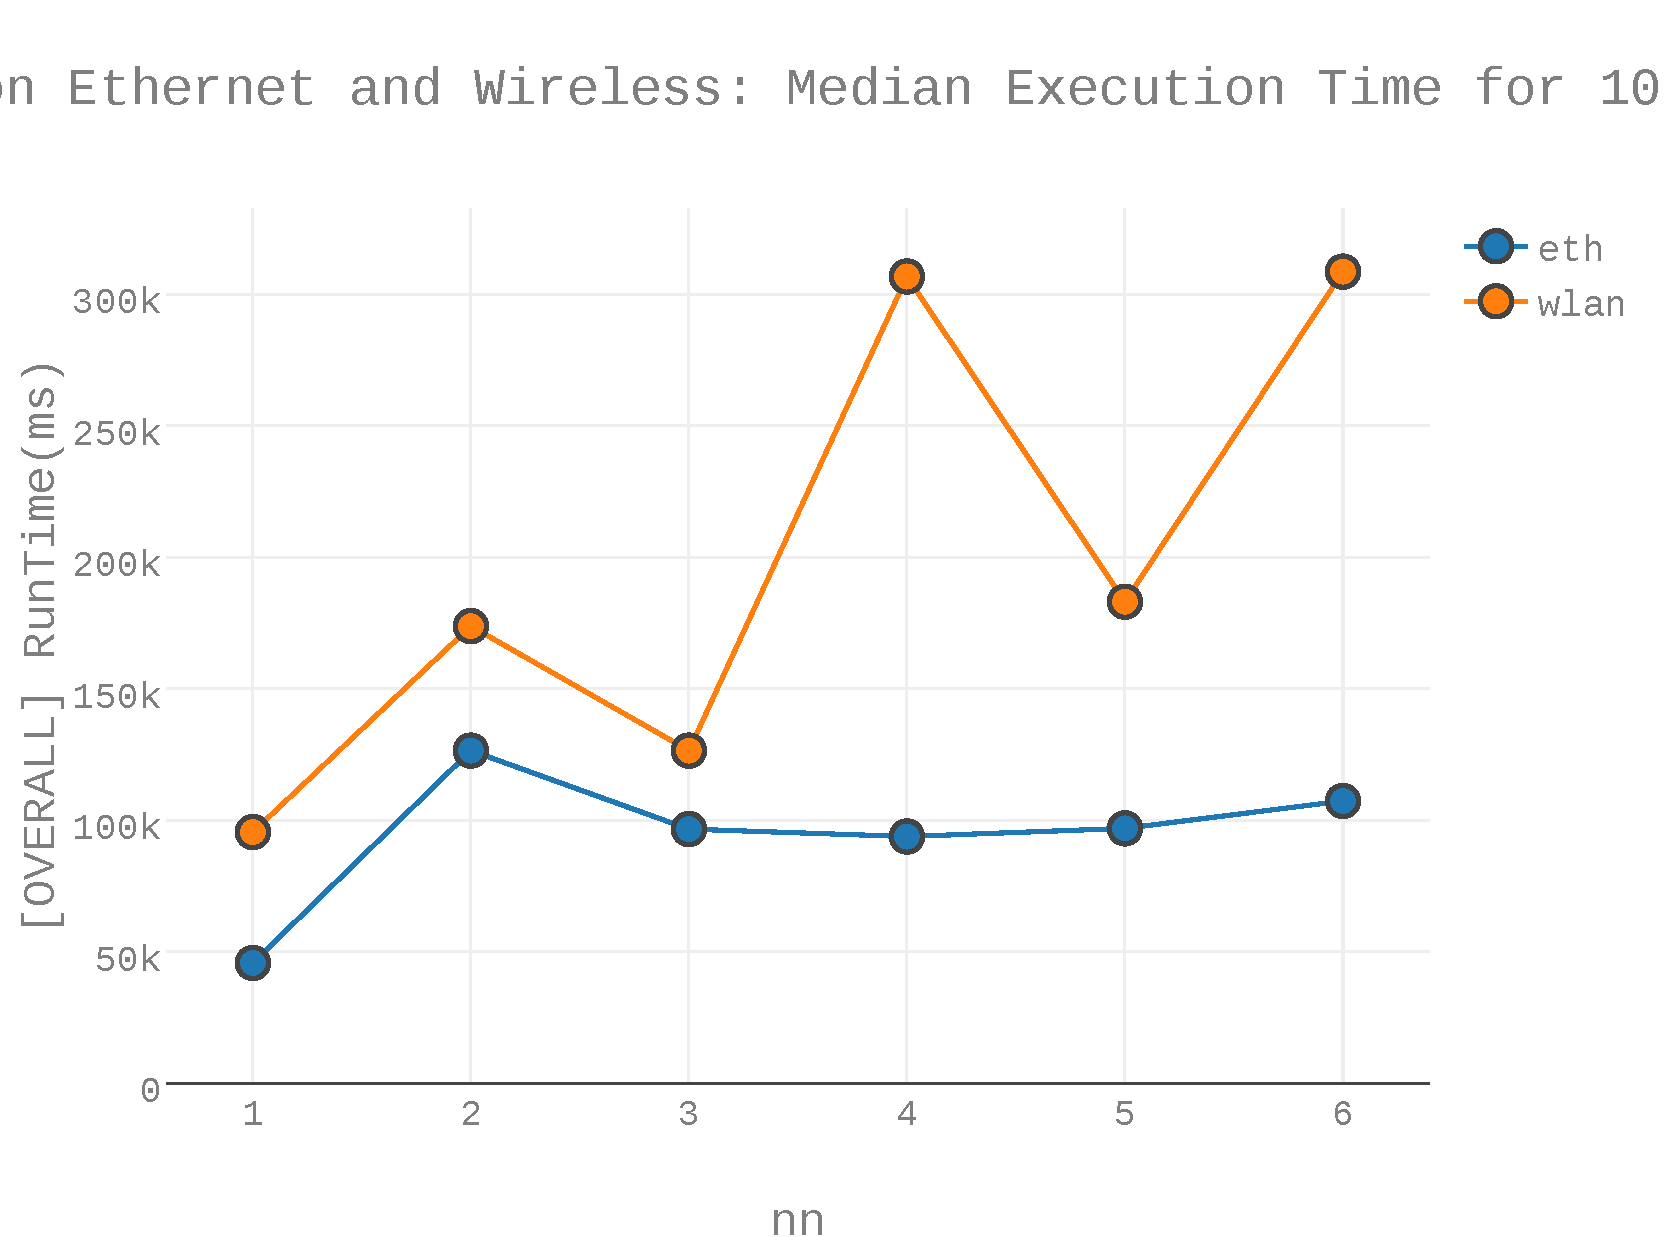
\includegraphics[width=3.5in]{Figures/figures-wla_fig7.pdf}

\caption{Comparison between the Ethernet links (eth) and wireless links (wlan) using the Raspberry Pi nodes.}

\label{fig:fig07}
\end{figure}

Figure \ref{fig:fig07} depicts the two experiments using Raspberry Pis: a wireless LAN (wlan) and an Ethernet LAN (eth).  In Figure \ref{fig:fig07}, as well as previous graphs, one can observe that the the Ethernet LAN effects about 50 seconds of execution time for 10,000 operations.  The initial median execution time for a node on a wireless LAN was found to be double the execution time.

For both configurations, performance takes a hit when transitioning from 1 to 2 nodes, but then increases from 2 nodes to 3 nodes.  From 3 nodes to 4 nodes, the wireless LAN configuration’s performance decreases dramatically, compared to slight increase in the wired Ethernet case.  

\begin{figure}[h]
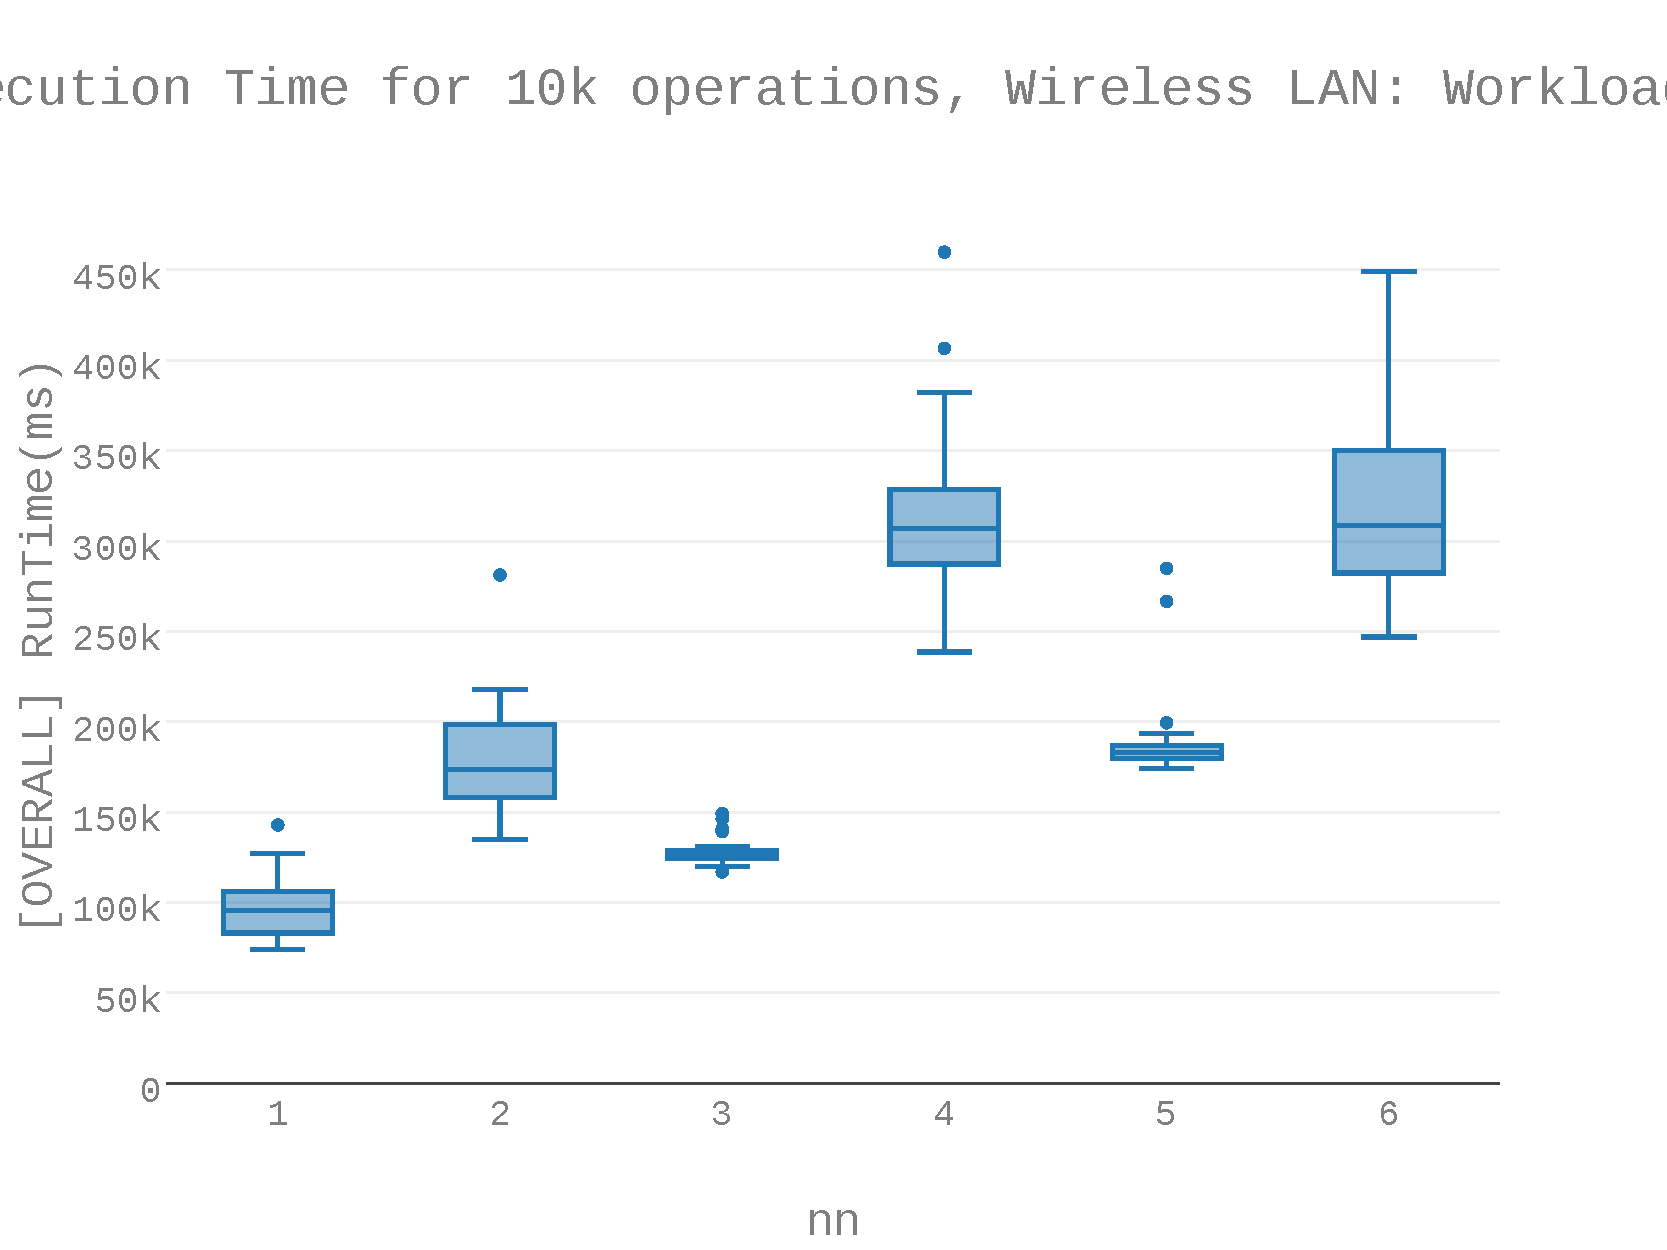
\includegraphics[width=3.5in]{Figures/figures-wla_fig8.pdf}

\caption{Distribution for all 30 trials of execution times where the Raspberry Pi nodes were connected via a wireless \gls{lan}.  Suspected outliers, values more than 3 times the interquartile range, are included as individual points above and below the 'maximum' and 'minimum' bars.}

\label{fig:fig08}
\end{figure}

A summary representation box plot of the results of wireless experimentation is above.  Here, the laptop was connected to the router via an Ethernet cable, and each node was connected to the router on a wireless local area network (LAN).  Suspected outliers, values more than 3 times the interquartile range (IQR) are included as points above and below.
There seems to be an overall increasing trend, while the data seems to oscillate, performing better for odd (1,3,5 node) configurations than for even (2,4,6 node) configurations.  However, there is no current theory behind this anomaly. 

\begin{figure}[h]
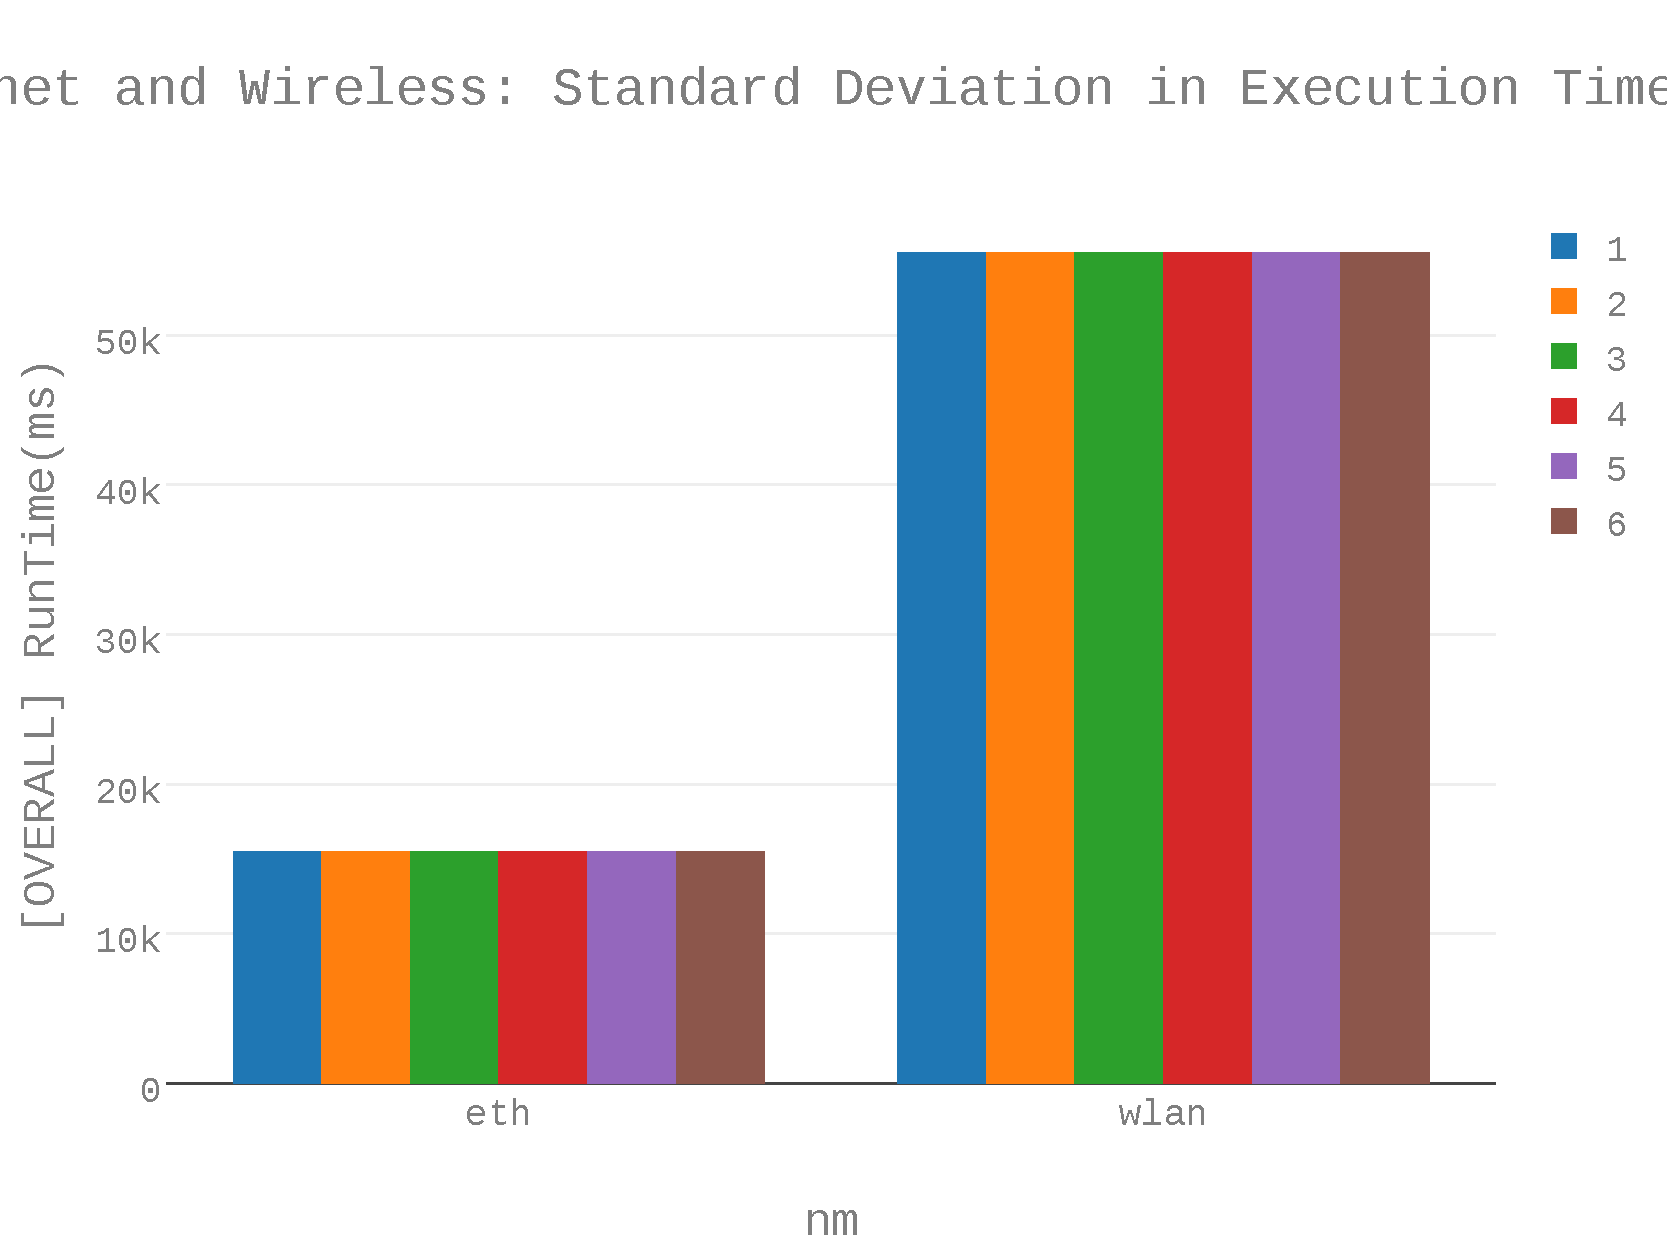
\includegraphics[width=3.5in]{Figures/figures-wla_fig9.pdf}

\caption{This compares the standard deviation in execution times for 10,000 operations of Workload A on the wired (eth) versus the wireless (wlan) configurations for 1 node, 2 nodes, 3 nodes, up through 6 nodes in milliseconds.}

\label{fig:fig09}
\end{figure}

To supplement the box plot, the standard deviation execution times for each set of trials, separated by number of nodes, is depicted in Figure \ref{fig:fig09}.  The difference seen here appears stark, and is overwhelming compared to the variance between 1, 2, 3, 4, 5 and 6 node networks given the same communication method. 

%1)      Reduced performance of Workload A is not statistically significant for the reduced memory sizes of IoT like devices
%2)      When varying platforms, performance for Workload A tracks the performance of the reference paper. For trials performe, reduced performance of Workload A is within 100ms of the reference paper (abramova) for wired implementations.
%3)      When varying communication method, reduced performance of Workload A is within 100ms of the wired platform test (order of magnitude, no greater than 100% increase in delay)
%4)      Reduced performance of Workload C is not statistically significant for the reduced memory sizes of IoT like devices
%5)      When varying platforms, reduced performance of Workload C is within 100ms of the reference paper (abramova) for wired implementations
%6)      When varying communication method, reduced performance of Workload C is within 100ms of the wired platform test
%7)      Reduced performance of Workload E is not statistically significant for the reduced memory sizes of IoT like devices
%8)      When varying platforms, reduced performance of Workload E is within 100ms of the reference paper (abramova) for wired implementations
%9)      When varying communication method, reduced performance of Workload E is within 100ms of the wired platform test

%\section{Results - Research Question 2}

\subsection{Comparing Existing Work}

\begin{figure}[h]
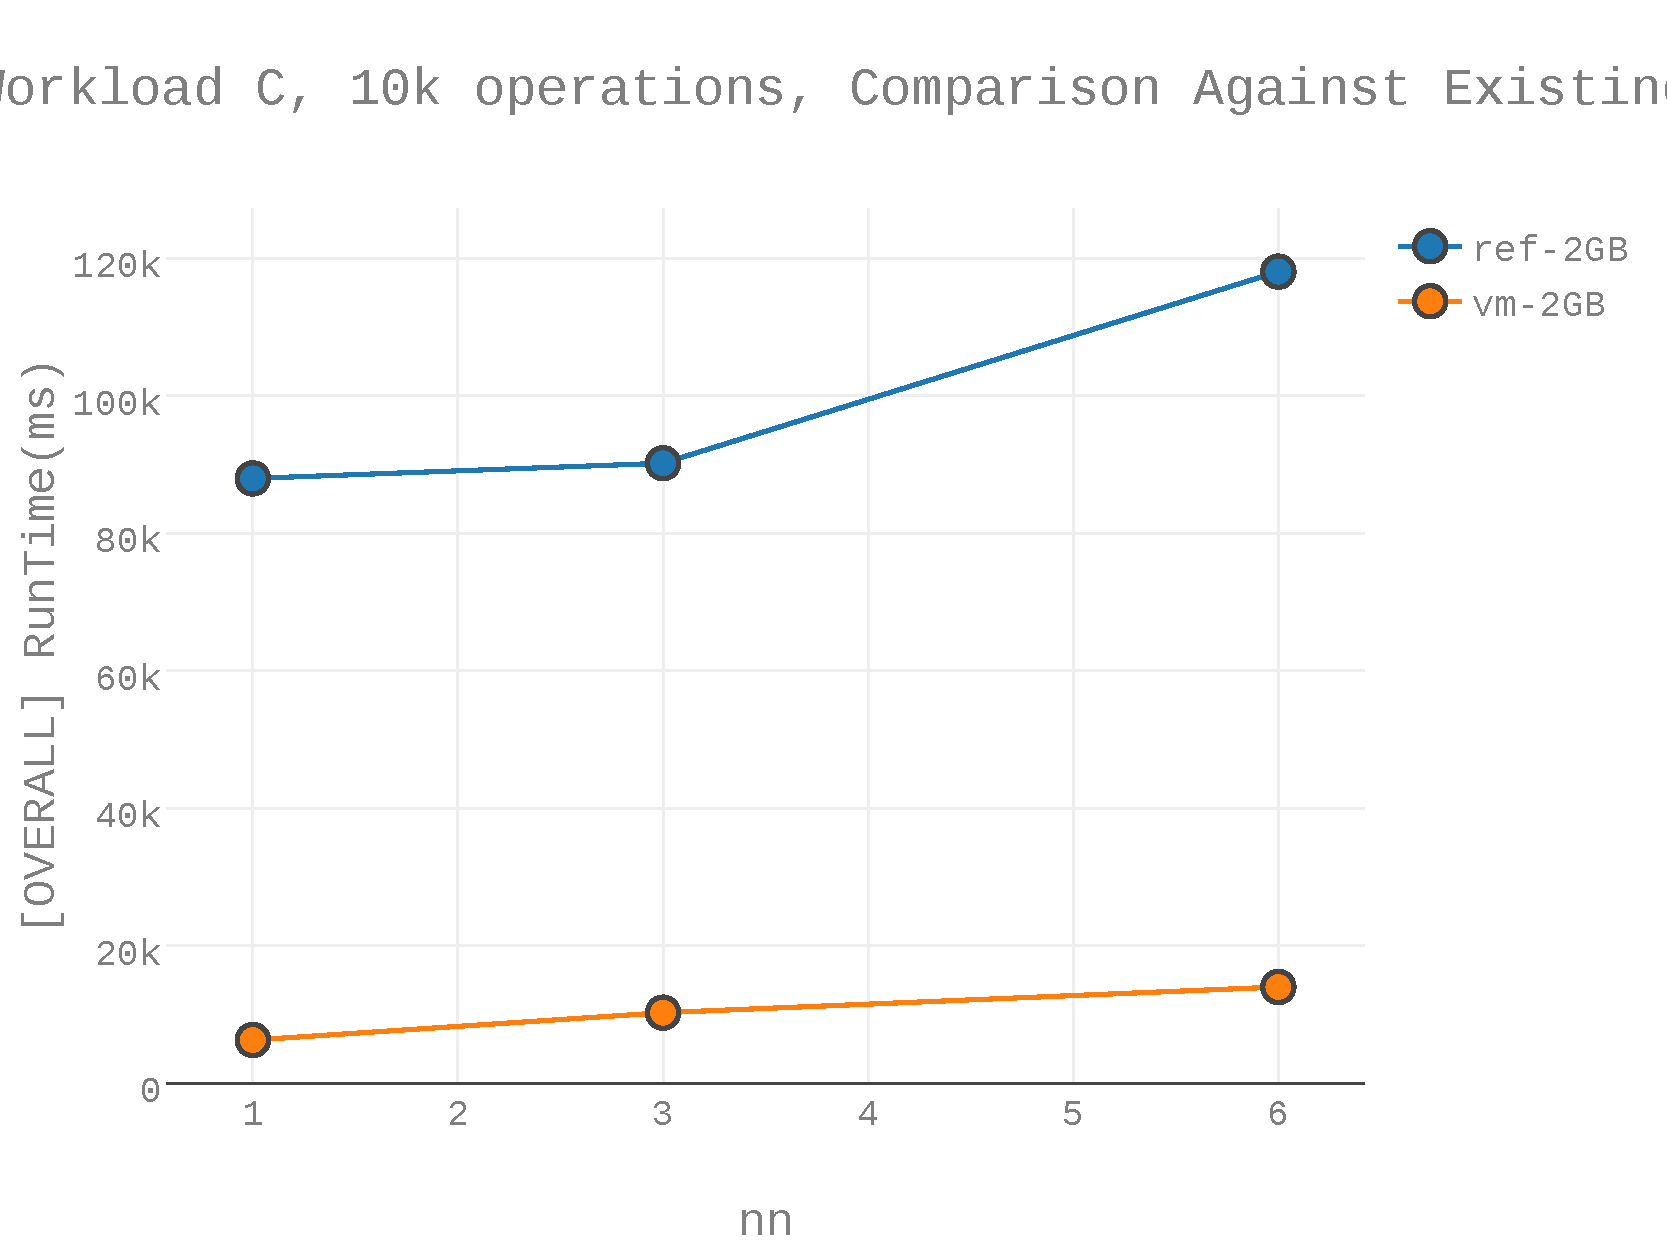
\includegraphics[width=3.5in]{Figures/figures-wlc_fig5.pdf}

\caption{Comparing the results in \cite{Abramova2014} with the median value of the virtual machine assigned 2GB of \gls{ram}.  Note that the virtual machines were on a nodal network (minimal propagation delay) while the the links in \cite{Abramova2014} were unspecified.}

\label{fig:figures-wlc_fig5}
\end{figure}

Here, as depicted in \ref{fig:figures-wlc_fig5}, one can see that the virtual machine configured to represent the network in \cite{Abramova2014} appears to perform at a significantly shorter execution time compared to the work done in \cite{Abramova2014}, probably largely due to the fact that the networks are nodal and do not experience any significant propagation delay compared, what could be inferred to be, a physical Ethernet cable.

The summary for the 2GB virtual node are in Tables \ref{table:summary_statistics_for_1_config}, \ref{table:summary_statistics_for_3_config}, and \ref{table:summary_statistics_for_6_config} under 'ram2GB'.  

One would expect, given that once this is extended to the Raspberry Pi modules require some kind of physical network connection (Ethernet) and a 900 MHz processor compared to the 2.90 GHz processor used by the virtual machines, the performance would be represented by significantly longer execution time.  

Facing minimal propagation delay due to being connected on a nodal network, experiments with the virtual machines seek to place an upper limit on potential \gls{iot} performance expectations, which for this analysis translates to a floor on timing.  Additional conventions would be necessary to find any sort of universal floor on Cassandra, but for the experiments, the results from running experiments on the virtual machines.

\subsection{Testing various memory sizes}

We now discuss testing and performance for memory sizes ranging from 1GB to 4GB.  The experience with 512MB was documented with Workload A.

\subsubsection{Experimental Testing for Memory in the 1GB – 4GB Range}

This section describes the results of running the \gls{ycsb} on virtual node networks as described in the methodology.  The summary of execution times are reported in Tables \ref{table:summary_statistics_for_1_config}, \ref{table:summary_statistics_for_3_config}, and \ref{table:summary_statistics_for_6_config}.  For each table, the summary statistics are listed for each amount of memory.

\paragraph{Visual Inspection of Results}

It is best to start with a visual inspection of the data represented in Figure \ref{fig:figures-wlc_fig4}.  Generally the greater amount of \gls{ram}, the fewer problems one would have with memory overloads, or needing to compact. However, for each sample, it seems that different amount of memory yields the best performance.

If there was a hint that 4GB performs better than 2GB, or 2GB performs better than 1GB, or both, this might be cause to attempt a regression to form a preliminary predictive model.  However, from first glance, it appears that an further examination of the data will indicate that the amount of memory does not independently predict performance, forming the null hypothesis of the \gls{anova} test to come.

\begin{figure}[h]
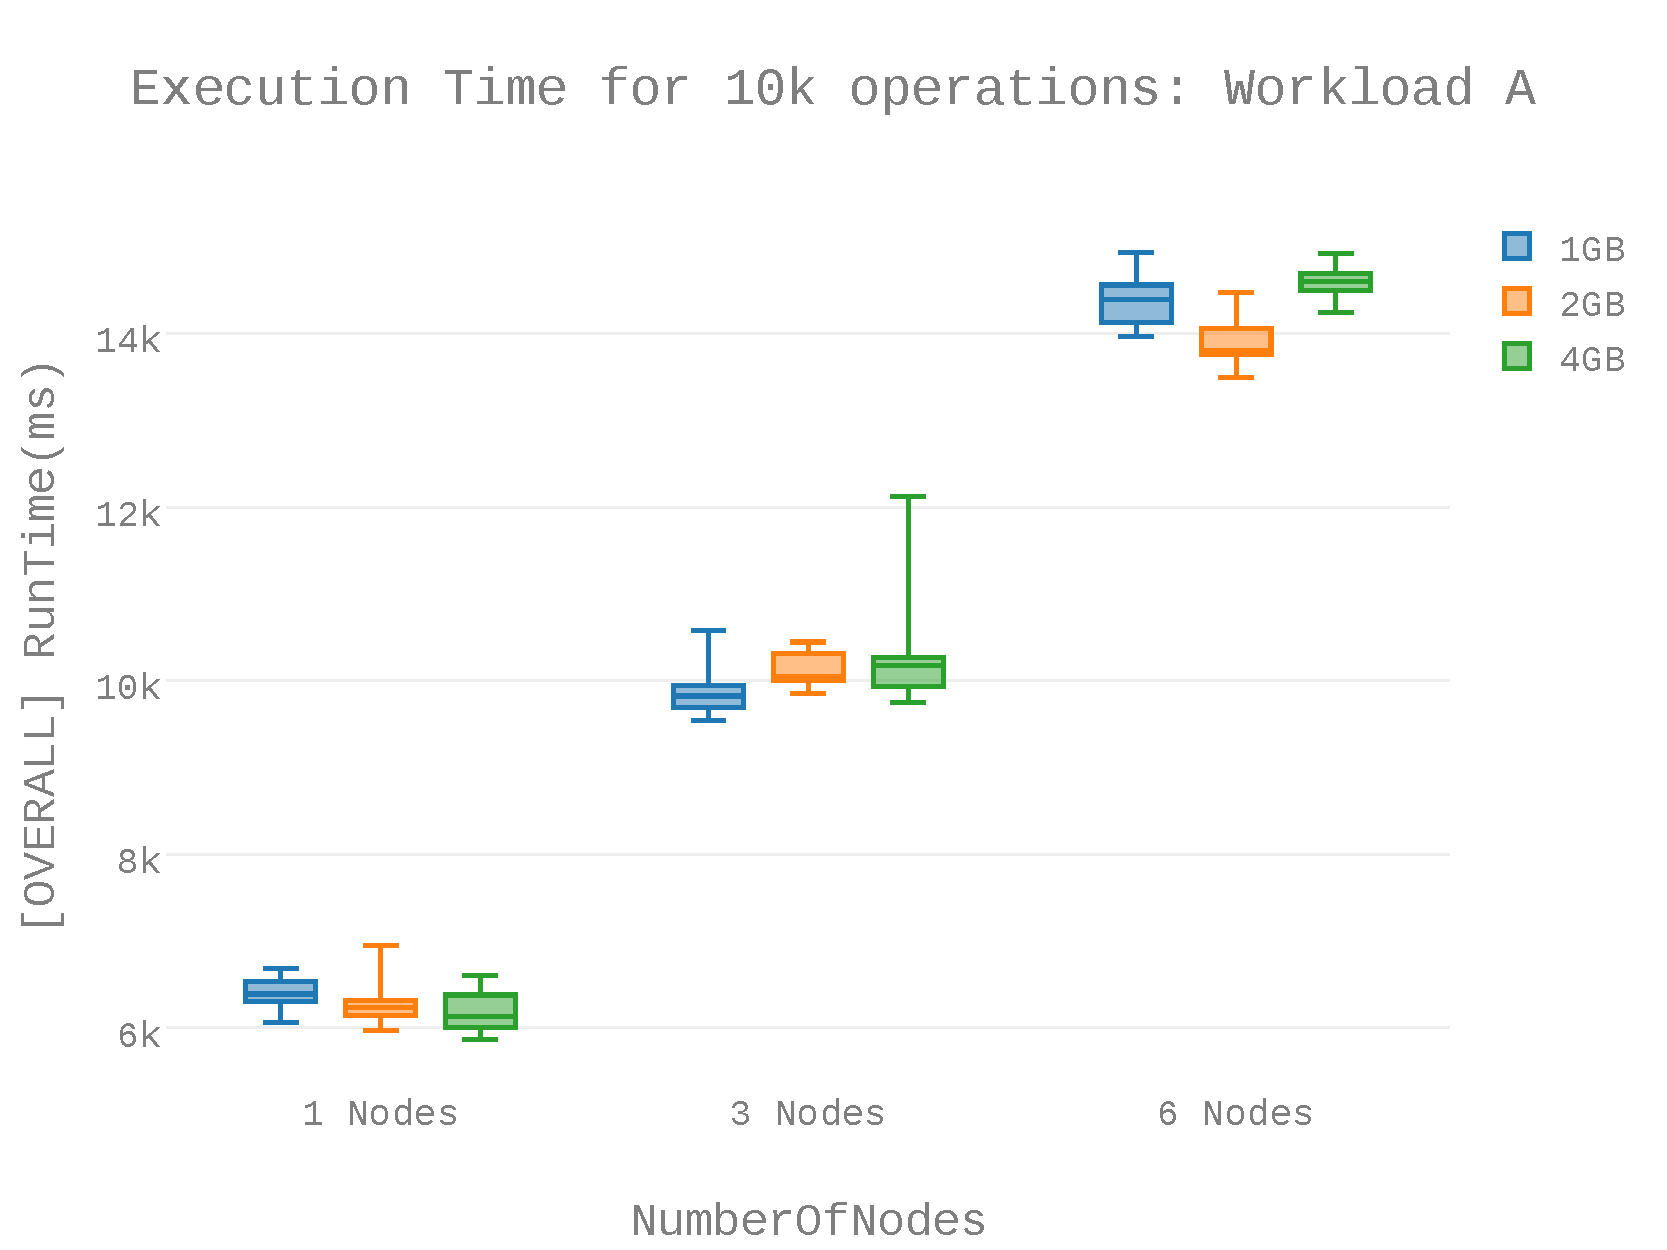
\includegraphics[width=3.5in]{Figures/figures-wlc_fig4.pdf}

\caption{Execution time for virtual machines with 1GB, 2GB, and 4GB of \gls{ram}.  The first 9 trials have been removed in order to filter out the trials representing the cache effect and thus represent the steady state.}

\label{fig:figures-wlc_fig4}
\end{figure}
\begin{table}
\begin{tabular}{lrrr}
\toprule
 index &  ram1GB &  ram2GB &  ram4GB \\
\midrule
 count &      21 &      21 &      21 \\
  mean & 6404.62 & 6263.71 &    6179 \\
   std & 165.241 & 221.031 & 231.934 \\
   min &    6057 &    5966 &    5865 \\
   25\% &    6304 &    6152 &    6017 \\
   50\% &    6391 &    6230 &    6134 \\
   75\% &    6526 &    6306 &    6377 \\
   max &    6687 &    6946 &    6604 \\
 range &     630 &     980 &     739 \\
\bottomrule
\end{tabular}
\caption{Summary Statistics for 1-Node Configuration. All values represented fall between 5865.0 ms and 6946.0 ms, or rather within a span of 1081.0 ms.}
\label{table:summary_statistics_for_1_config}
\end{table}
\begin{table}
\begin{tabular}{lrrr}
\toprule
 index &  ram1GB &  ram2GB &  ram4GB \\
\midrule
 count &      21 &      21 &      21 \\
  mean & 9878.24 & 10139.6 & 10215.5 \\
   std & 255.122 & 180.863 & 495.567 \\
   min &    9542 &    9849 &    9753 \\
   25\% &    9695 &   10009 &    9935 \\
   50\% &    9823 &   10049 &   10176 \\
   75\% &    9929 &   10307 &   10263 \\
   max &   10578 &   10445 &   12126 \\
 range &    1036 &     596 &    2373 \\
\bottomrule
\end{tabular}
\caption{Summary Statistics for 3-Node Configuration. All values represented fall between 9542.0 ms and 12126.0 ms, or rather within a span of 2584.0 ms.}
\label{table:summary_statistics_for_3_config}
\end{table}
\begin{table}
\begin{tabular}{lrrr}
\toprule
 index &  ram1GB &  ram2GB &  ram4GB \\
\midrule
 count &      21 &      21 &      21 \\
  mean & 14373.4 & 13910.4 & 14586.3 \\
   std & 302.838 & 263.331 & 180.081 \\
   min &   13962 &   13491 &   14242 \\
   25\% &   14137 &   13763 &   14496 \\
   50\% &   14388 &   13808 &   14601 \\
   75\% &   14551 &   14020 &   14690 \\
   max &   14938 &   14468 &   14924 \\
 range &     976 &     977 &     682 \\
\bottomrule
\end{tabular}
\caption{Summary Statistics for 6-Node Configuration. All values represented fall between 13491.0 ms and 14938.0 ms, or rather within a span of 1447.0 ms.}
\label{table:summary_statistics_for_6_config}
\end{table}

\paragraph{Absolute Ranges}

While Figure \ref{fig:figures-wlc_fig4} gives a general sense of what the results look like, the actual summary statistics can be examined in Tables \ref{table:summary_statistics_for_1_config}, \ref{table:summary_statistics_for_3_config}, and \ref{table:summary_statistics_for_6_config}. After filtering out the first nine trials, the results for running 10,000 operations is displayed in Tables \ref{table:summary_statistics_for_1_config}, \ref{table:summary_statistics_for_3_config}, and \ref{table:summary_statistics_for_6_config}.  For each configuration, varying the \gls{ram} of the virtual machine resulted in execution times that fell within 2 seconds of each other.

\paragraph{\gls{anova}}

A one-way \gls{anova} was performed with the filtered data, and the \gls{anova} summary tables can be seen in Tables \ref{ram_variance_analysis_workload_a_1_node}, \ref{ram_variance_analysis_workload_a_3_node}, and \ref{ram_variance_analysis_workload_a_6_node} for the 1, 3, and 6 node cases respectively.  For each case, the  p-value is much, much less than 0.05, and thus it can be said that one can be 95\% confident in the decision to fail to reject the null hypothesis, the hypothesis that the means are equal.

\begin{table}
\begin{tabular}{lrrrrr}
\toprule
         Source &            SS &  df &             MS &         F &         p \\
\midrule
 between groups &  5.455423e+05 &   2 &  272771.158730 &  6.297012 &  0.003292 \\
  within groups &  2.599053e+06 &  60 &   43317.553968 &       NaN &       NaN \\
          total &  3.144596e+06 &  62 &            NaN &       NaN &       NaN \\
\bottomrule
\end{tabular}
\caption{ANOVA Summary Table for Workload C, 1 Node}
\label{table:ram_variance_analysis_workload_c_1_node}
\end{table}

\begin{table}
\begin{tabular}{lrrrrr}
\toprule
         Source &            SS &  df &             MS &         F &         p \\
\midrule
 between groups &  1.314779e+06 &   2 &  657389.349207 &  5.743313 &  0.005221 \\
  within groups &  6.867702e+06 &  60 &  114461.703175 &       NaN &       NaN \\
          total &  8.182481e+06 &  62 &            NaN &       NaN &       NaN \\
\bottomrule
\end{tabular}
\caption{ANOVA Summary Table for Workload C, 3 Node}
\label{table:ram_variance_analysis_workload_c_3_node}
\end{table}

\begin{table}
\begin{tabular}{lrrrrr}
\toprule
         Source &            SS &  df &            MS &          F &             p \\
\midrule
 between groups &  5.015054e+06 &   2 &  2.507527e+06 &  38.879796 &  1.482116e-11 \\
  within groups &  3.869660e+06 &  60 &  6.449434e+04 &        NaN &           NaN \\
          total &  8.884714e+06 &  62 &           NaN &        NaN &           NaN \\
\bottomrule
\end{tabular}
\caption{ANOVA Summary Table for Workload C, 6 Node}
\label{table:ram_variance_analysis_workload_c_6_node}
\end{table}

Examining the effects of variance in the amount of \gls{ram} allocated the virtual machines does not seem to have a notable impact on performance.  This indicates that, any observed limitation on the Raspberry Pis’ performance is not limited by \gls{ram}, but something else, and that varying \gls{ram} in future tests will not yield significant results.

% Insert something about statistical significance

\subsection{Implementation on Raspberry Pi}

In a similar fashion, the tests were run on the Raspberry Pi to observe performance.  The spread of each of the tests can be seen in Figure \ref{fig:wlc_fig10} and Table \ref{table:wired-results}.  The results, next to one trend for the virtual machines, can be seen in Figure \ref{fig:fig06}. 

\begin{figure}[h]
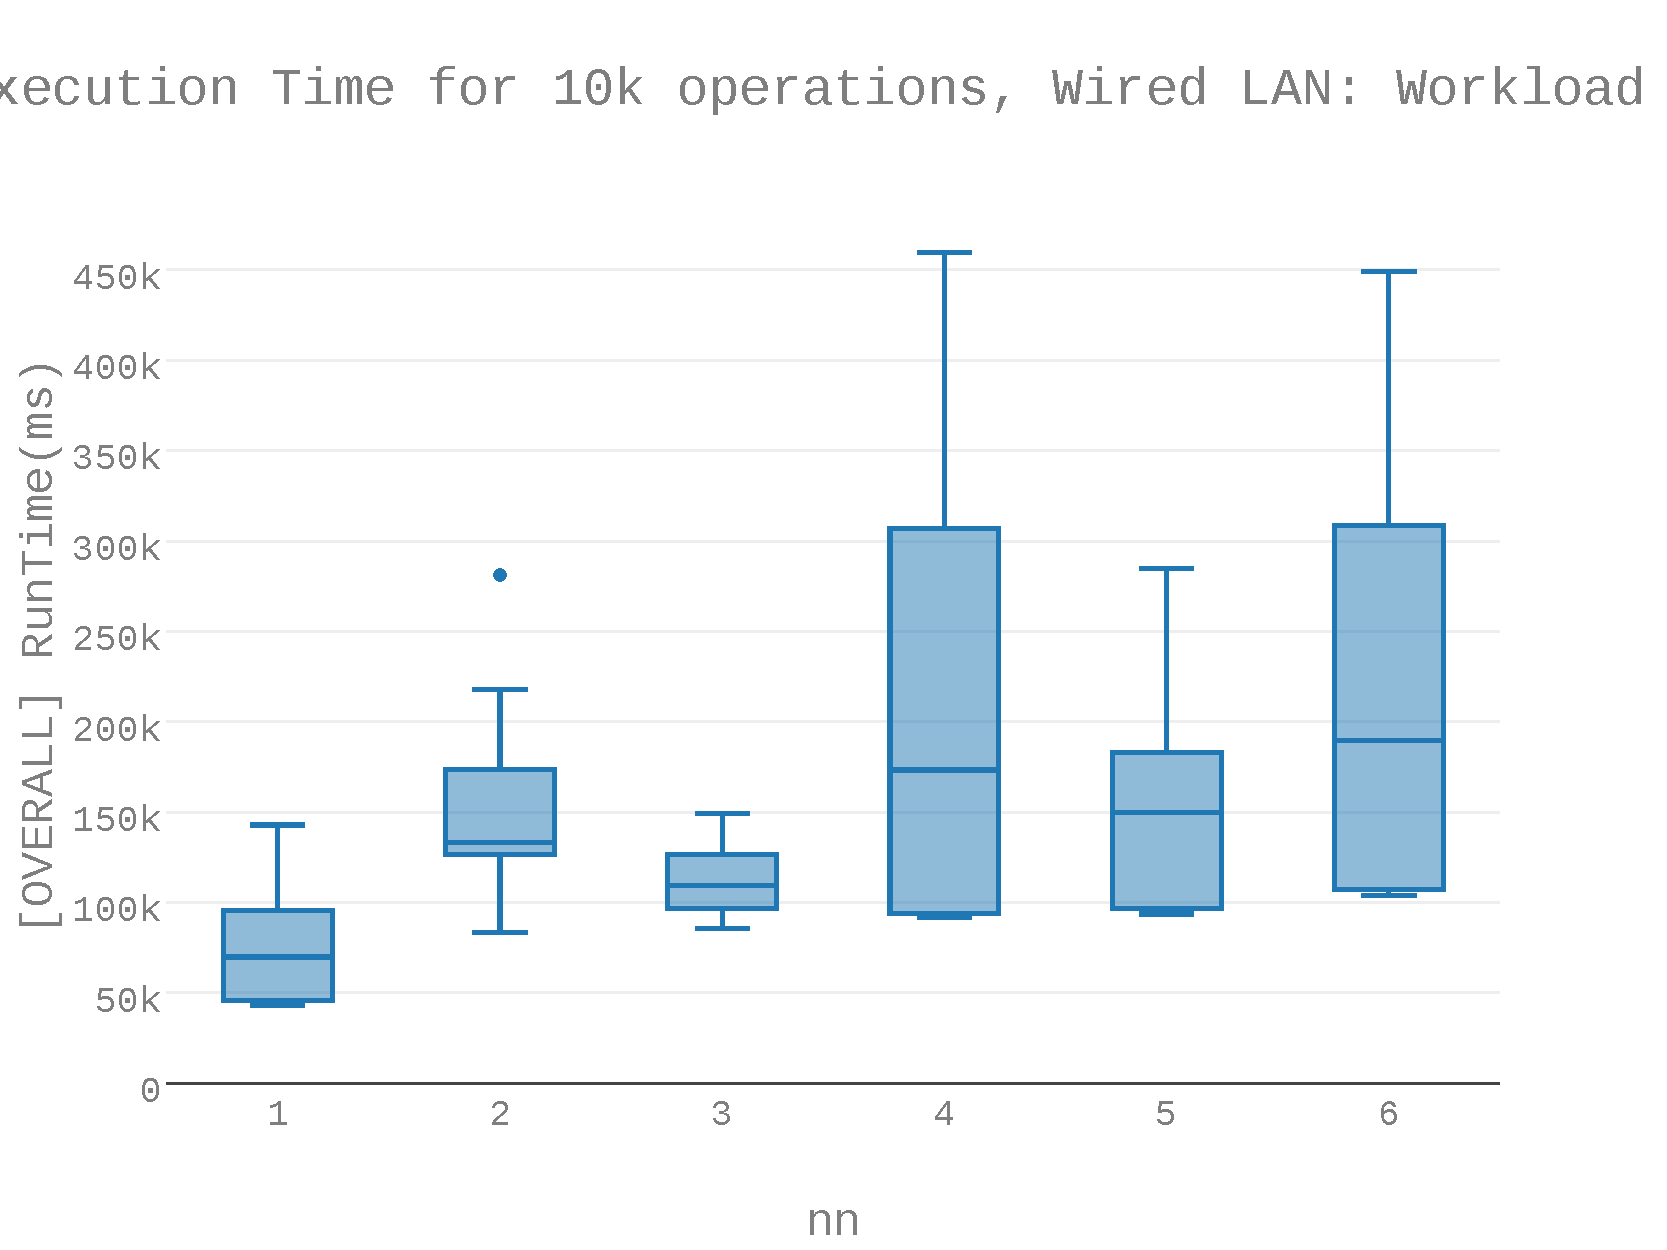
\includegraphics[width=3.5in]{Figures/figures-wlc_fig10.pdf}

\caption{Box plot representing the results of the workload applied to wired local area network on the Raspberry Pi platform.}

\label{fig:wlc_fig10}
\end{figure}

\begin{figure}[h]
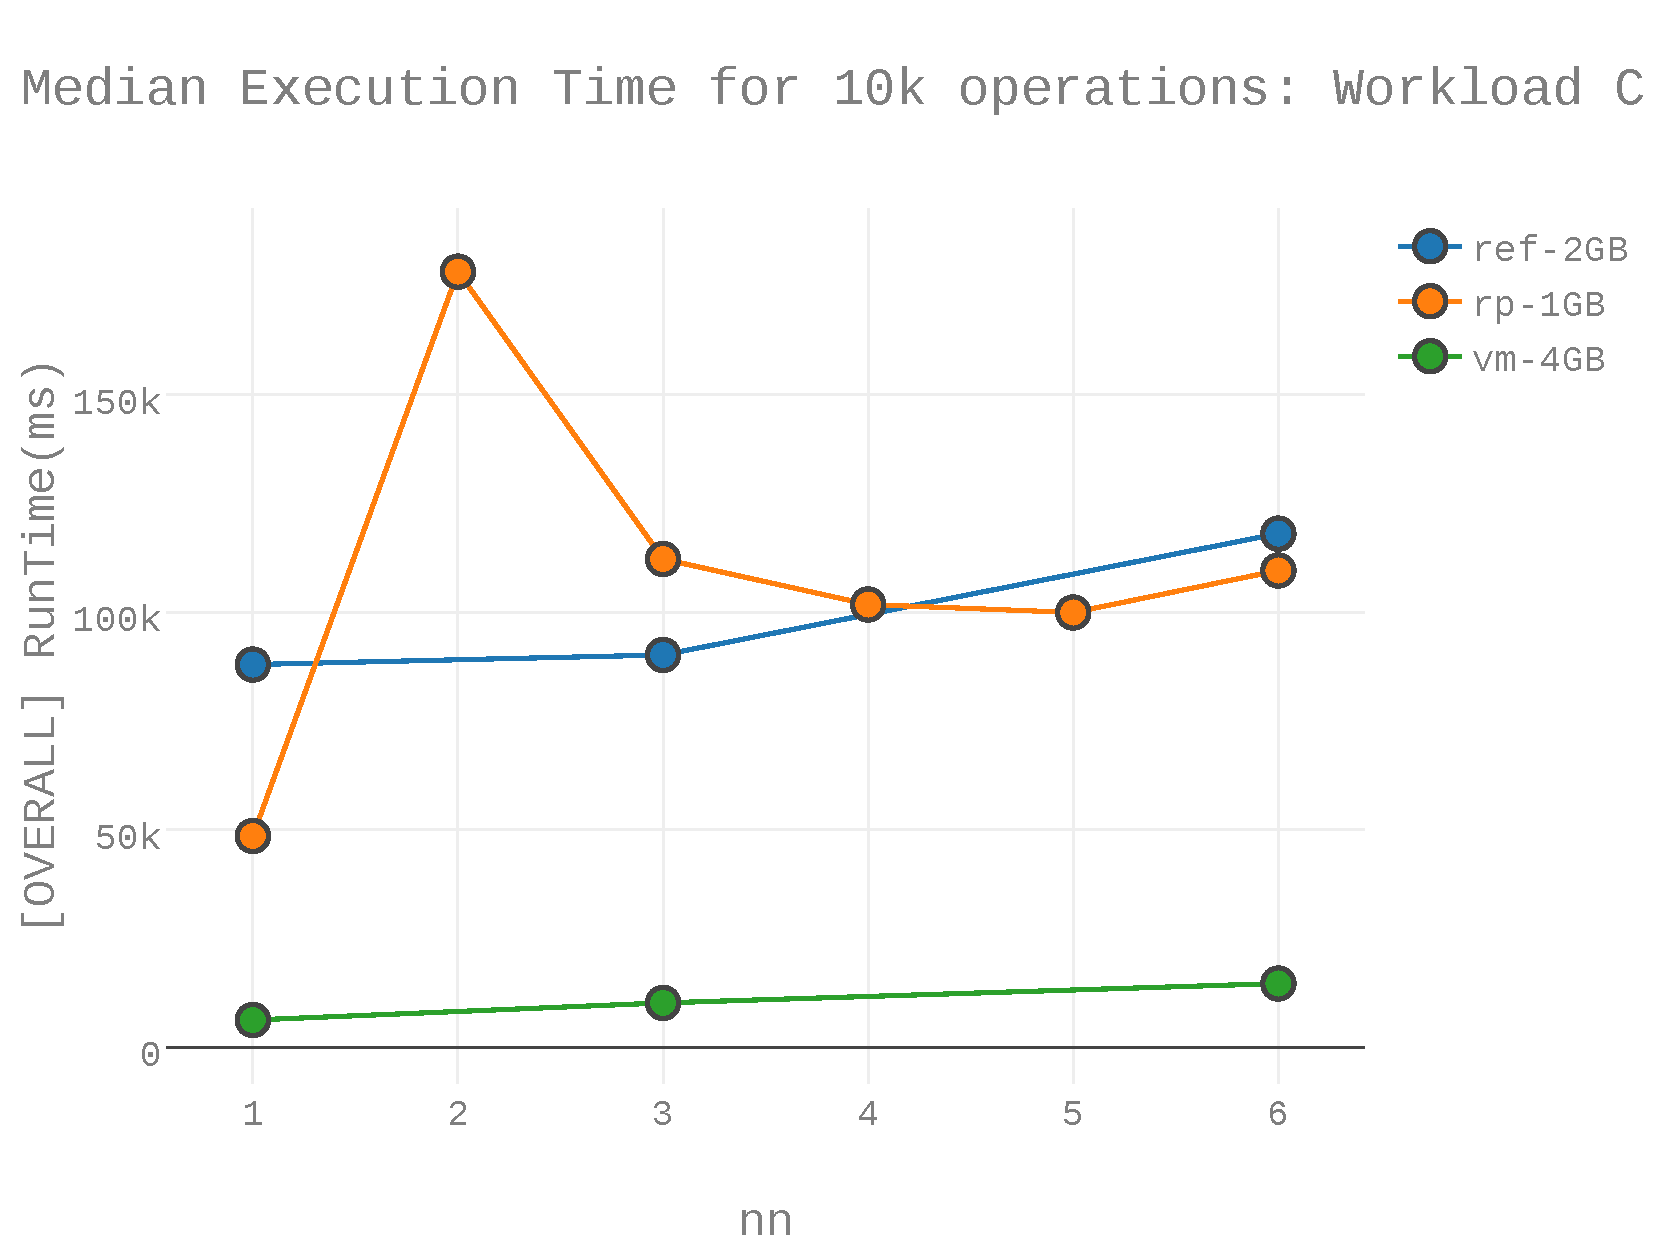
\includegraphics[width=3.5in]{Figures/figures-wlc_fig6.pdf}

\caption{Comparison between the Raspberry Pi nodes (rp-1GB), the results reported in \cite{Abramova2014} (ref-2GB), and the virtual nodes with 4GB available \gls{ram} (vm-4GB).}

\label{fig:fig06}
\end{figure}

\begin{table}
\begin{tabular}{lrrr}
\toprule
 index &       1 &       3 &       6 \\
\midrule
 count &      21 &      21 &      21 \\
  mean & 4.8e+04 & 1.1e+05 & 1.1e+05 \\
   std & 1.8e+03 & 3.2e+03 & 2.1e+03 \\
   min & 4.5e+04 & 1.1e+05 &   1e+05 \\
   25\% & 4.7e+04 & 1.1e+05 & 1.1e+05 \\
   50\% & 4.9e+04 & 1.1e+05 & 1.1e+05 \\
   75\% &   5e+04 & 1.1e+05 & 1.1e+05 \\
   max &   5e+04 & 1.3e+05 & 1.1e+05 \\
 range & 5.4e+03 & 1.7e+04 & 8.1e+03 \\
\bottomrule
\end{tabular}
\caption{Summary for Raspberry Pi wired local area network}
\label{table:rp_wired_summary_statistics}
\end{table}

As can be seen from Figure \ref{fig:fig06}, the Raspberry Pi configuration takes considerably more execution time than the virtual machine analogy, which is probably due to the physical nature of the Ethernet connections (propagation delay) and the I/O limitations of the Raspberry Pi hardware.  However, its seemingly similar performance to the reference in \cite{Abramova2014} suggests the \gls{io} for the \gls{sd} Card follows a predictable pattern, and actually seems to outperform the node in \cite{Abramova2014} in the degenerate 1-node case.

For this paragraph, consider the results from \cite{Abramova2014} as the reference.  For a node network of 1, the experimental values fell between 43260.0 ms and 48123.0 ms, inclusive, and all values fell within 15170.0 ms of the reference value of 58430 ms.  For a node network of 3, the experimental values fell between 93702.0 ms and 100501.0 ms, inclusive, and all values fell within 34851.0 ms of the reference value of 65650 ms.  For a node network of 6, the experimental values fell between 103728.0 ms and 111002.0 ms, inclusive, and all values fell within 23692.0 ms of the reference value of 87310 ms.  

\subsection{Wireless Links}

The median value of the corresponding wired experiment will serve as the reference in this paragraph. For a node network of 1, the experimental values fell between 74072.0 ms and 119580.0 ms, inclusive, and all values fell within 73961.0 ms of the reference value of 45619.0 ms.  For a node network of 3, the experimental values fell between 123064.0 ms and 149252.0 ms, inclusive, and all values fell within 52156.0 ms of the reference value of 97096.0 ms.  For a node network of 6, the experimental values fell between 246945.0 ms and 355538.0 ms, inclusive, and all values fell within 248820.0 ms of the reference value of 106718.0 ms.

\begin{figure}[h]
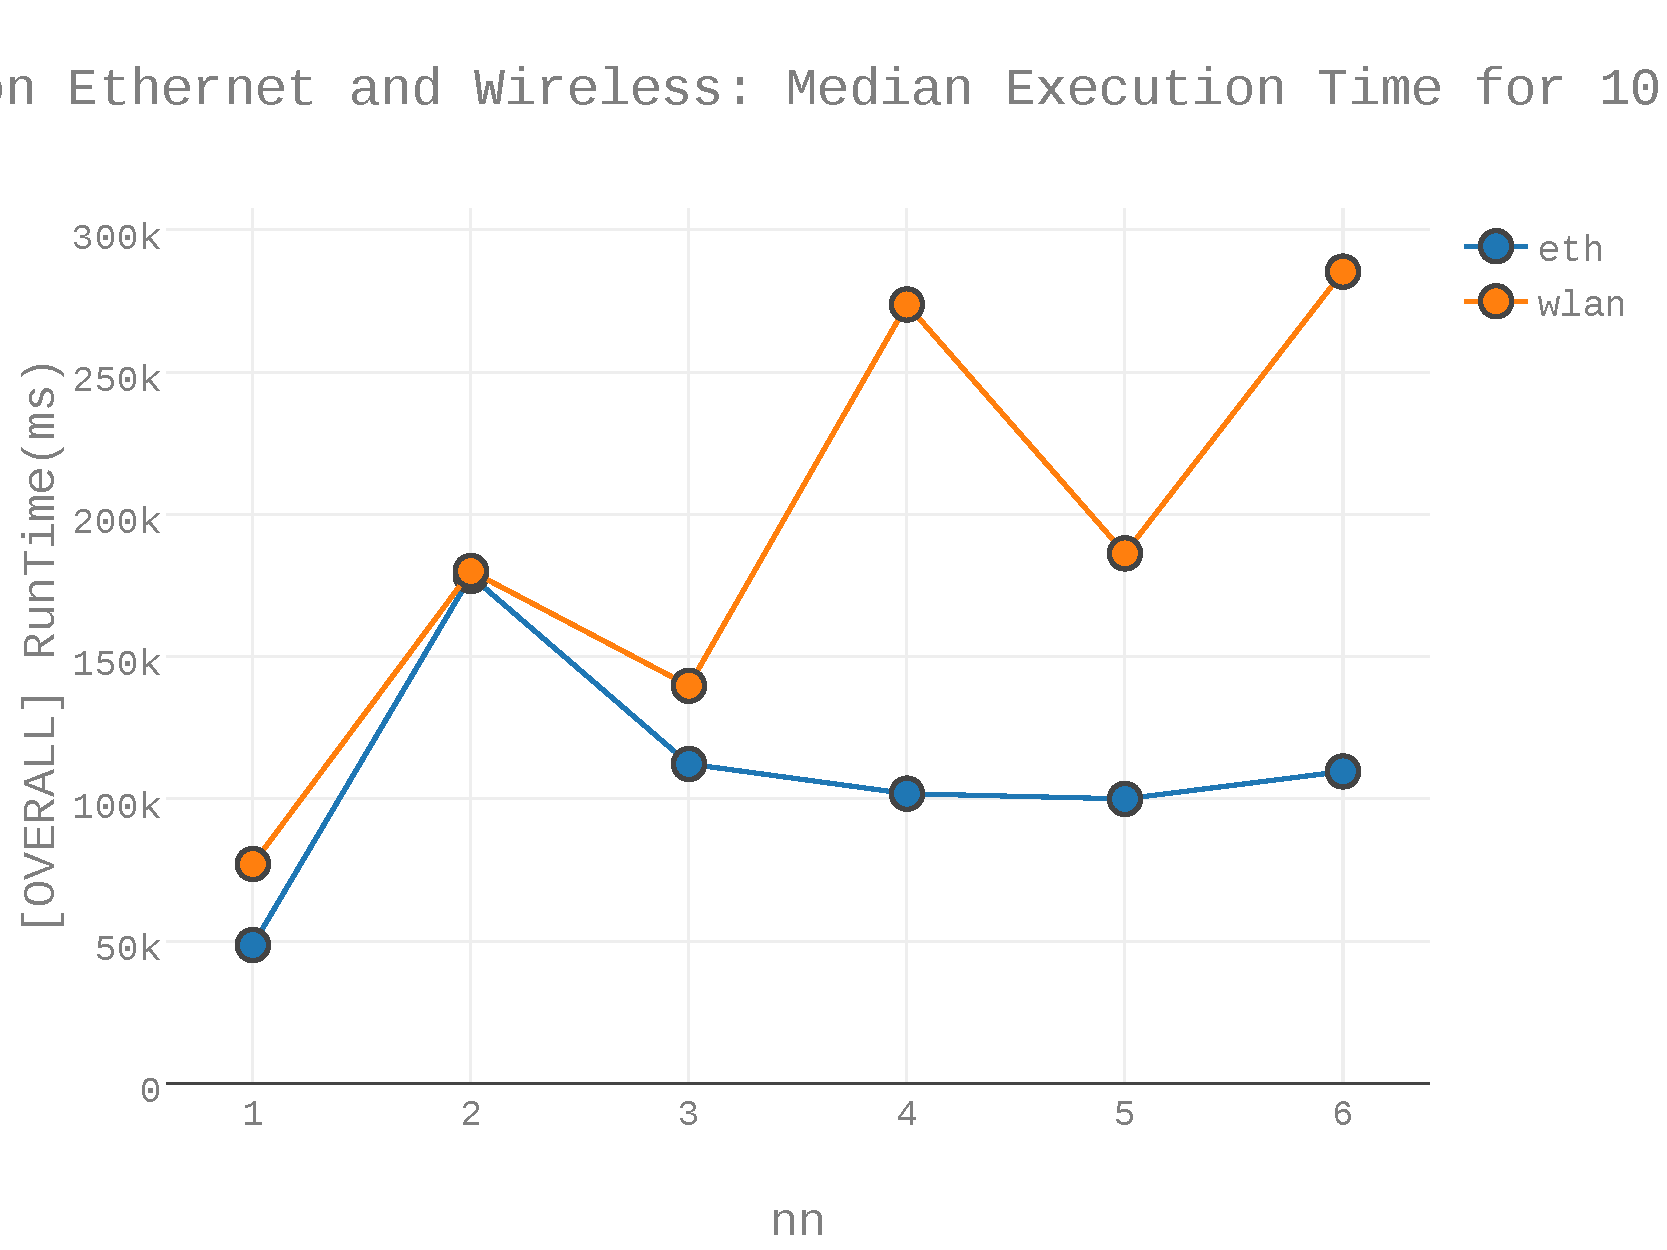
\includegraphics[width=3.5in]{Figures/figures-wlc_fig7.pdf}

\caption{Comparison between the Ethernet links (eth) and wireless links (wlan) using the Raspberry Pi nodes.}

\label{fig:fig07}
\end{figure}

Figure \ref{fig:fig07} depicts the two experiments using Raspberry Pis: a wireless LAN (wlan) and an Ethernet LAN (eth).  In Figure \ref{fig:fig07}, as well as previous graphs, one can observe that the the Ethernet LAN effects about 50 seconds of execution time for 10,000 operations.  The initial median execution time for a node on a wireless LAN was found to be double the execution time.

For both configurations, performance takes a hit when transitioning from 1 to 2 nodes, but then increases from 2 nodes to 3 nodes.  From 3 nodes to 4 nodes, the wireless LAN configuration’s performance decreases dramatically, compared to slight increase in the wired Ethernet case.  

\begin{figure}[h]
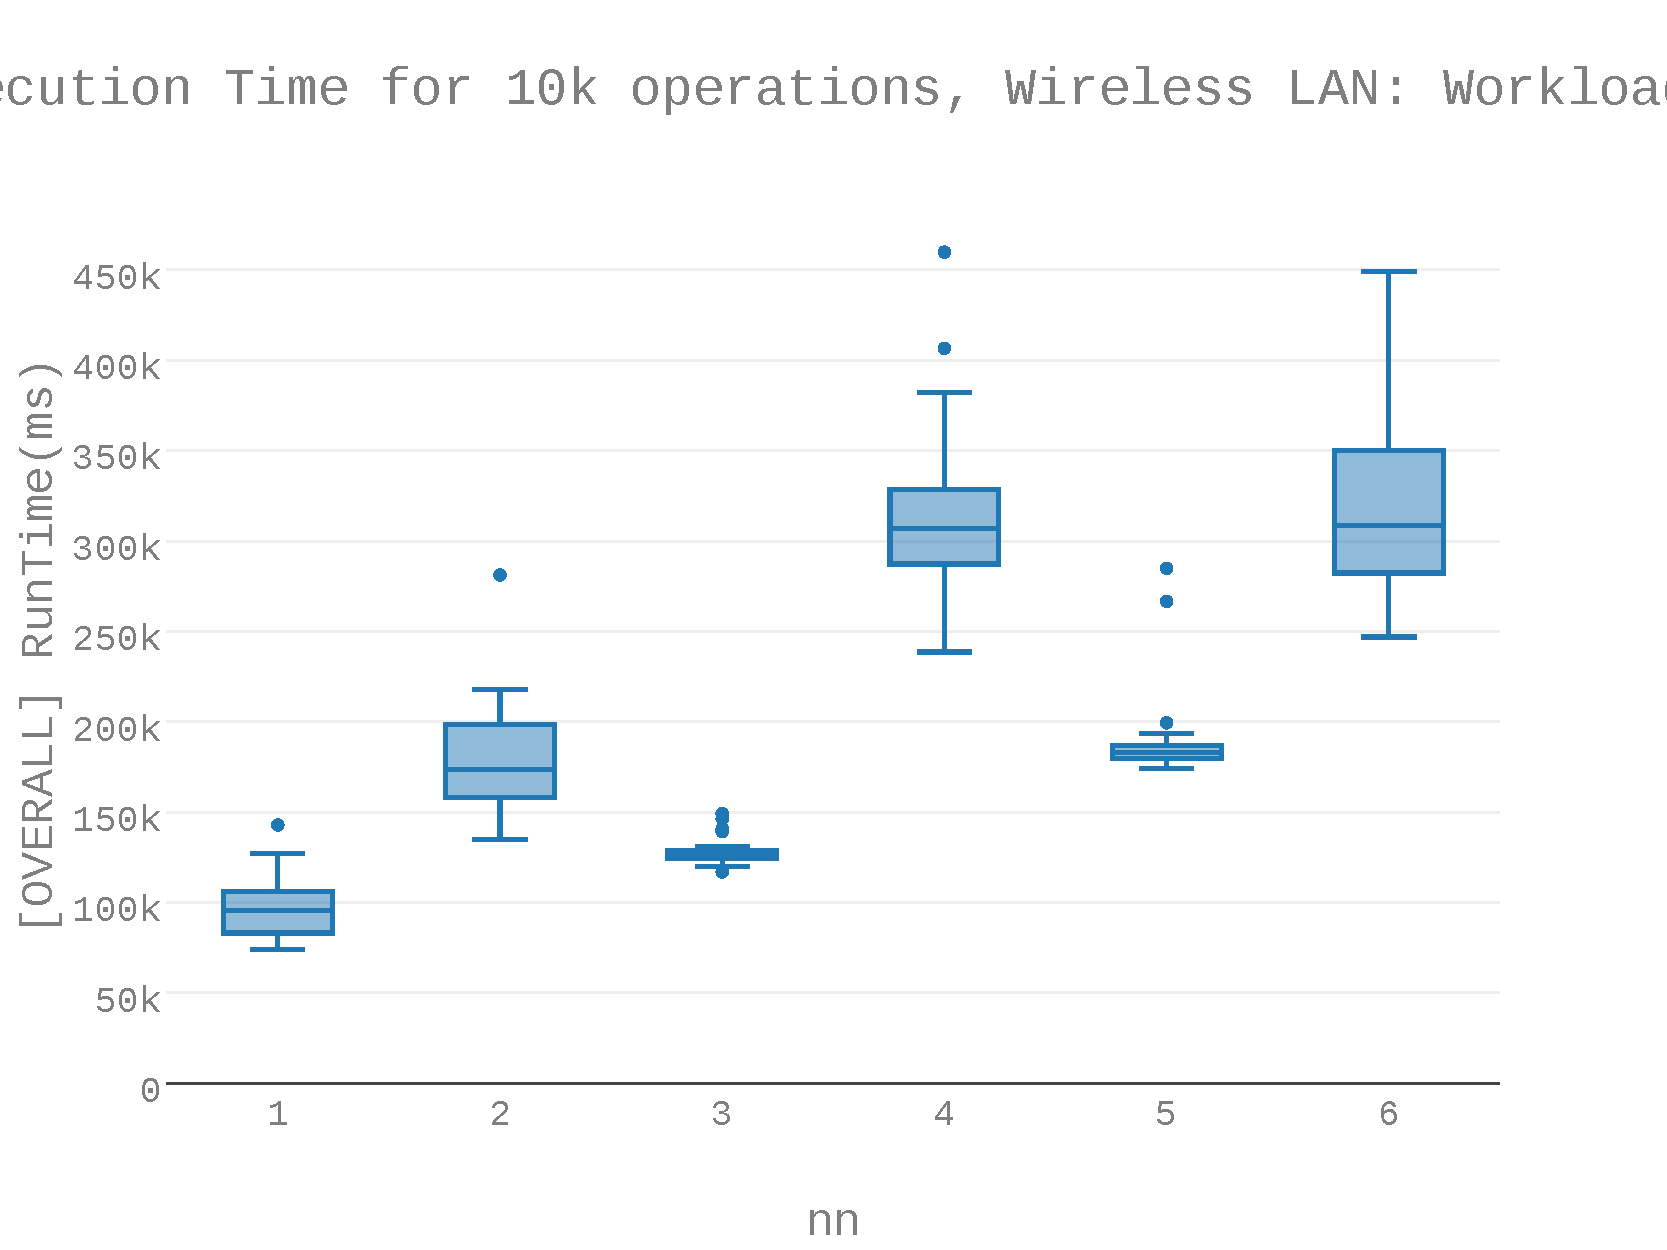
\includegraphics[width=3.5in]{Figures/figures-wlc_fig8.pdf}

\caption{Distribution for all 30 trials of execution times where the Raspberry Pi nodes were connected via a wireless \gls{lan}.  Suspected outliers, values more than 3 times the interquartile range, are included as individual points above and below the 'maximum' and 'minimum' bars.}

\label{fig:fig08}
\end{figure}

A summary representation box plot of the results of wireless experimentation is above.  Here, the laptop was connected to the router via an Ethernet cable, and each node was connected to the router on a wireless local area network (LAN).  Suspected outliers, values more than 3 times the interquartile range (IQR) are included as points above and below.
There seems to be an overall increasing trend, while the data seems to oscillate, performing better for odd (1,3,5 node) configurations than for even (2,4,6 node) configurations.  However, there is no current theory behind this anomaly. 

\begin{figure}[h]
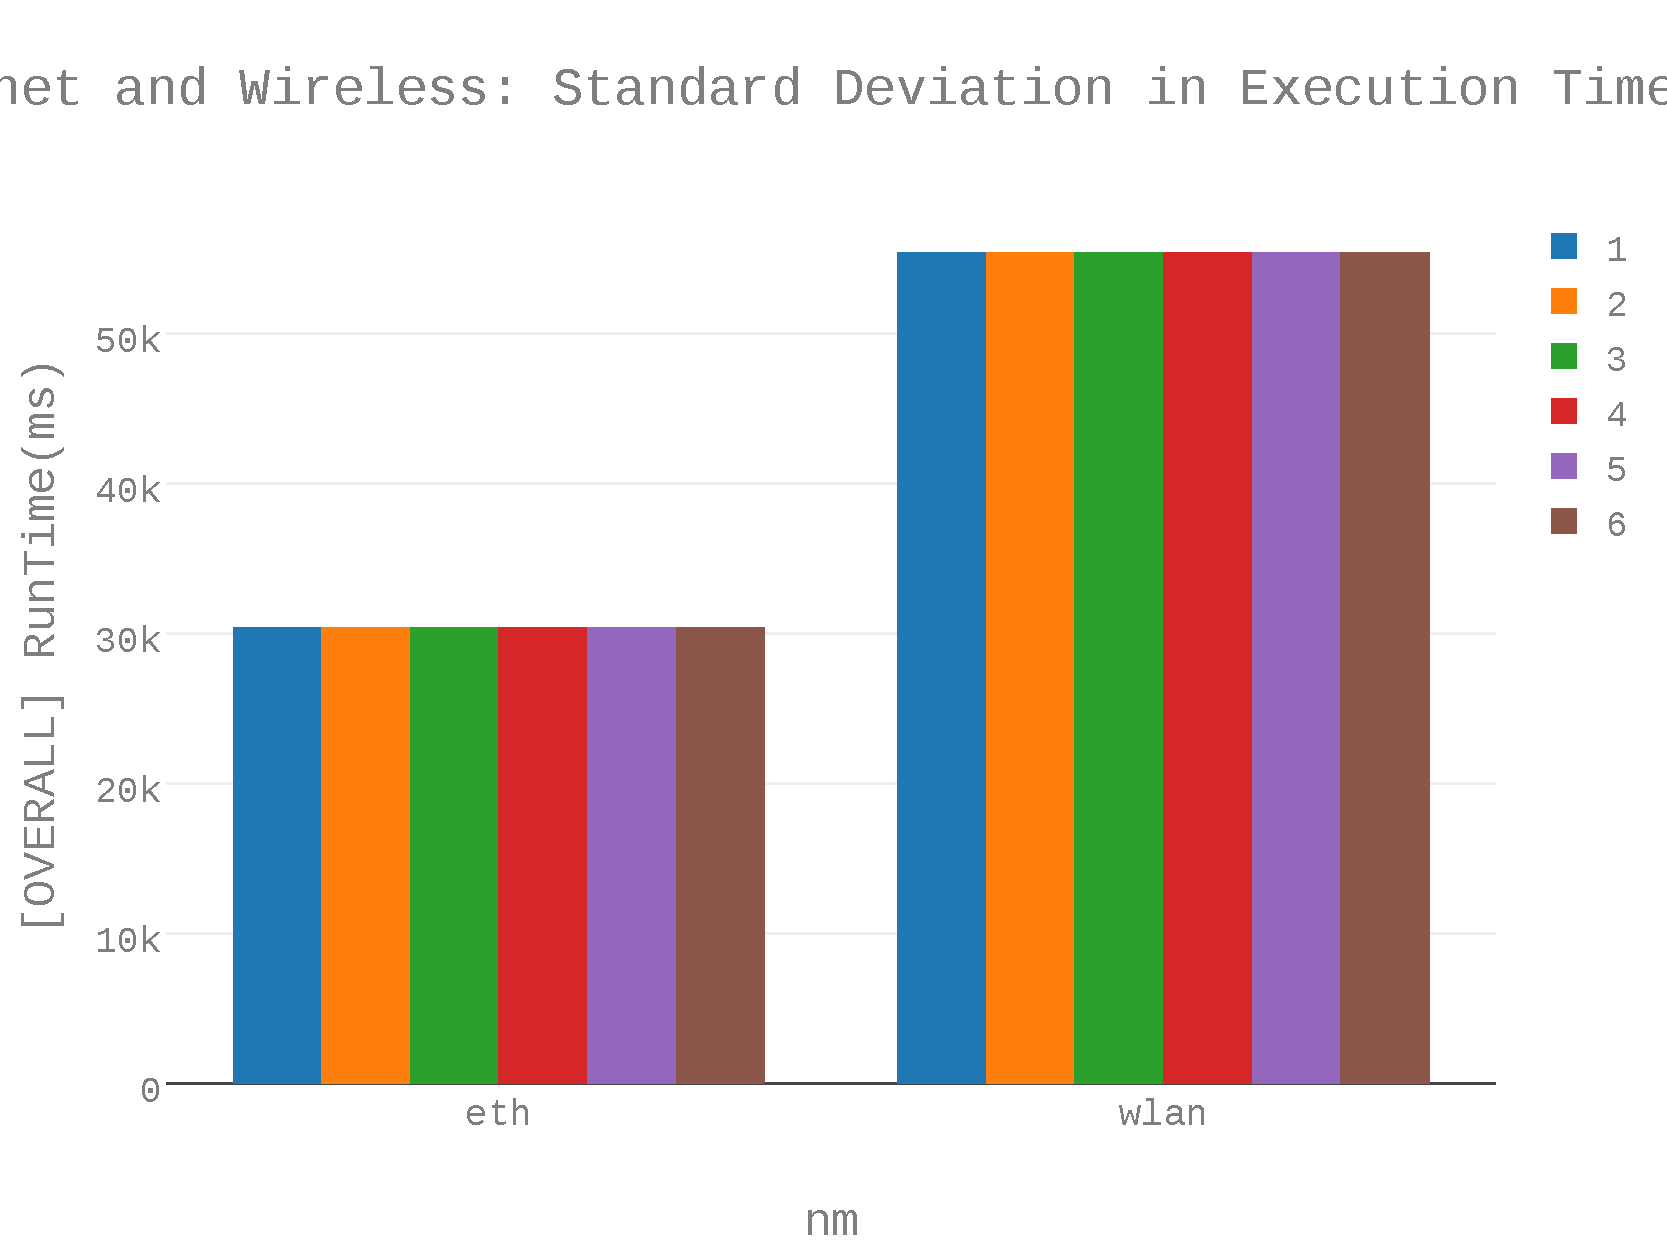
\includegraphics[width=3.5in]{Figures/figures-wlc_fig9.pdf}

\caption{This compares the standard deviation in execution times for 10,000 operations of Workload C on the wired (eth) versus the wireless (wlan) configurations for 1 node, 2 nodes, 3 nodes, up through 6 nodes in milliseconds.}

\label{fig:fig09}
\end{figure}

To supplement the box plot, the standard deviation execution times for each set of trials, separated by number of nodes, is depicted in Figure \ref{fig:fig09}.  The difference seen here appears stark, and is overwhelming compared to the variance between 1, 2, 3, 4, 5 and 6 node networks given the same communication method. 

%1)      Reduced performance of Workload A is not statistically significant for the reduced memory sizes of IoT like devices
%2)      When varying platforms, performance for Workload A tracks the performance of the reference paper. For trials performe, reduced performance of Workload A is within 100ms of the reference paper (abramova) for wired implementations.
%3)      When varying communication method, reduced performance of Workload A is within 100ms of the wired platform test (order of magnitude, no greater than 100% increase in delay)
%4)      Reduced performance of Workload C is not statistically significant for the reduced memory sizes of IoT like devices
%5)      When varying platforms, reduced performance of Workload C is within 100ms of the reference paper (abramova) for wired implementations
%6)      When varying communication method, reduced performance of Workload C is within 100ms of the wired platform test
%7)      Reduced performance of Workload E is not statistically significant for the reduced memory sizes of IoT like devices
%8)      When varying platforms, reduced performance of Workload E is within 100ms of the reference paper (abramova) for wired implementations
%9)      When varying communication method, reduced performance of Workload E is within 100ms of the wired platform test

%\section{Results - Research Question 3}

\subsection{Comparing Existing Work}

\begin{figure}[h]
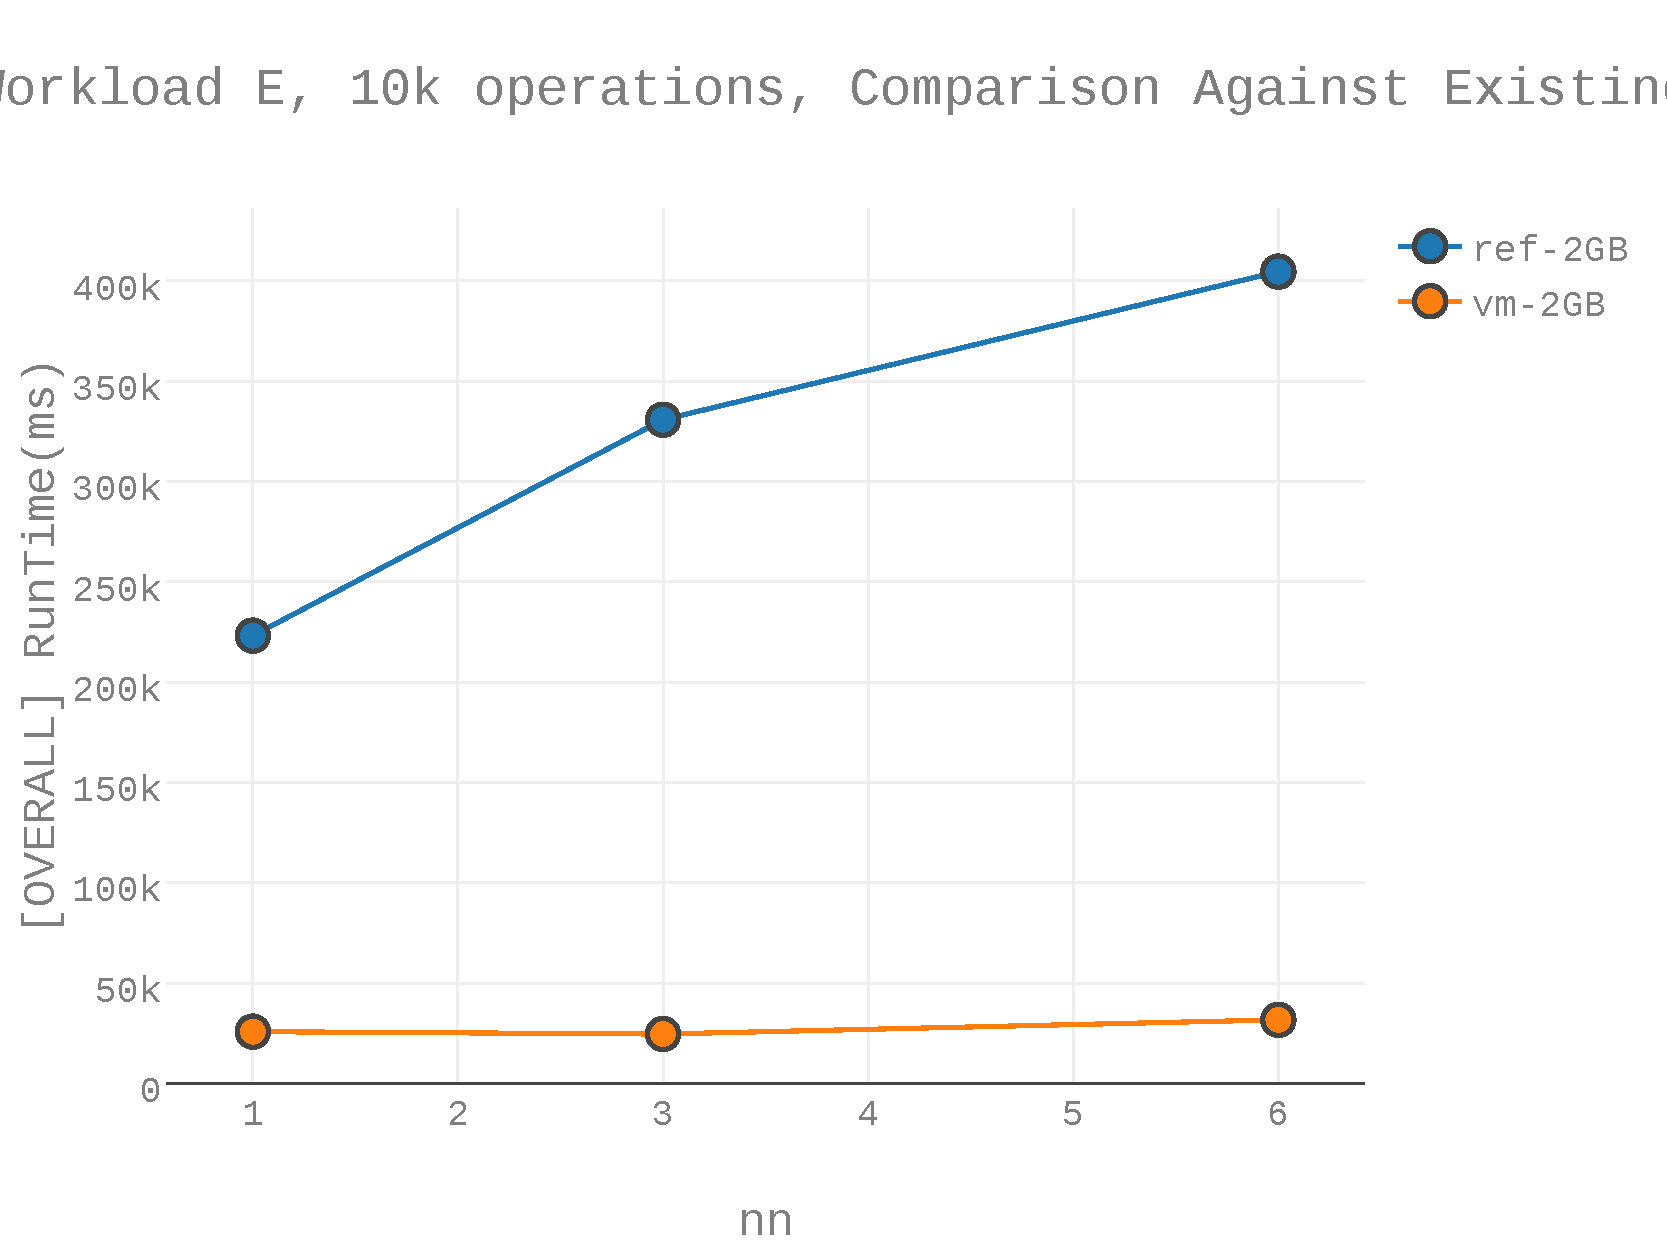
\includegraphics[width=3.5in]{Figures/figures-wle_fig5.pdf}

\caption{Comparing the results in \cite{Abramova2014} with the median value of the virtual machine assigned 2GB of \gls{ram}.  Note that the virtual machines were on a nodal network (minimal propagation delay) while the the links in \cite{Abramova2014} were unspecified.}

\label{fig:figures-wle_fig5}
\end{figure}

Here, as depicted in \ref{fig:figures-wle_fig5}, one can see that the virtual machine configured to represent the network in \cite{Abramova2014} appears to perform at a significantly shorter execution time compared to the work done in \cite{Abramova2014}, probably largely due to the fact that the networks are nodal and do not experience any significant propagation delay compared, what could be inferred to be, a physical Ethernet cable.

The summary for the 2GB virtual node are in Tables \ref{table:summary_statistics_for_1_config}, \ref{table:summary_statistics_for_3_config}, and \ref{table:summary_statistics_for_6_config} under 'ram2GB'.  

One would expect, given that once this is extended to the Raspberry Pi modules require some kind of physical network connection (Ethernet) and a 900 MHz processor compared to the 2.90 GHz processor used by the virtual machines, the performance would be represented by significantly longer execution time.  

Facing minimal propagation delay due to being connected on a nodal network, experiments with the virtual machines seek to place an upper limit on potential \gls{iot} performance expectations, which for this analysis translates to a floor on timing.  Additional conventions would be necessary to find any sort of universal floor on Cassandra, but for the experiments, the results from running experiments on the virtual machines.

\subsection{Testing various memory sizes}

We now discuss testing and performance for memory sizes ranging from 1GB to 4GB.  The experience with 512MB was documented with Workload A.

\subsubsection{Experimental Testing for Memory in the 1GB – 4GB Range}

This section describes the results of running the \gls{ycsb} on virtual node networks as described in the methodology.  The summary of execution times are reported in Tables \ref{table:summary_statistics_for_1_config}, \ref{table:summary_statistics_for_3_config}, and \ref{table:summary_statistics_for_6_config}.  For each table, the summary statistics are listed for each amount of memory.

\paragraph{Visual Inspection of Results}

It is best to start with a visual inspection of the data represented in Figure \ref{fig:figures-wle_fig4}.  Generally the greater amount of \gls{ram}, the fewer problems one would have with memory overloads, or needing to compact. However, for each sample, it seems that different amount of memory yields the best performance.

If there was a hint that 4GB performs better than 2GB, or 2GB performs better than 1GB, or both, this might be cause to attempt a regression to form a preliminary predictive model.  However, from first glance, it appears that an further examination of the data will indicate that the amount of memory does not independently predict performance, forming the null hypothesis of the \gls{anova} test to come.

\begin{figure}[h]
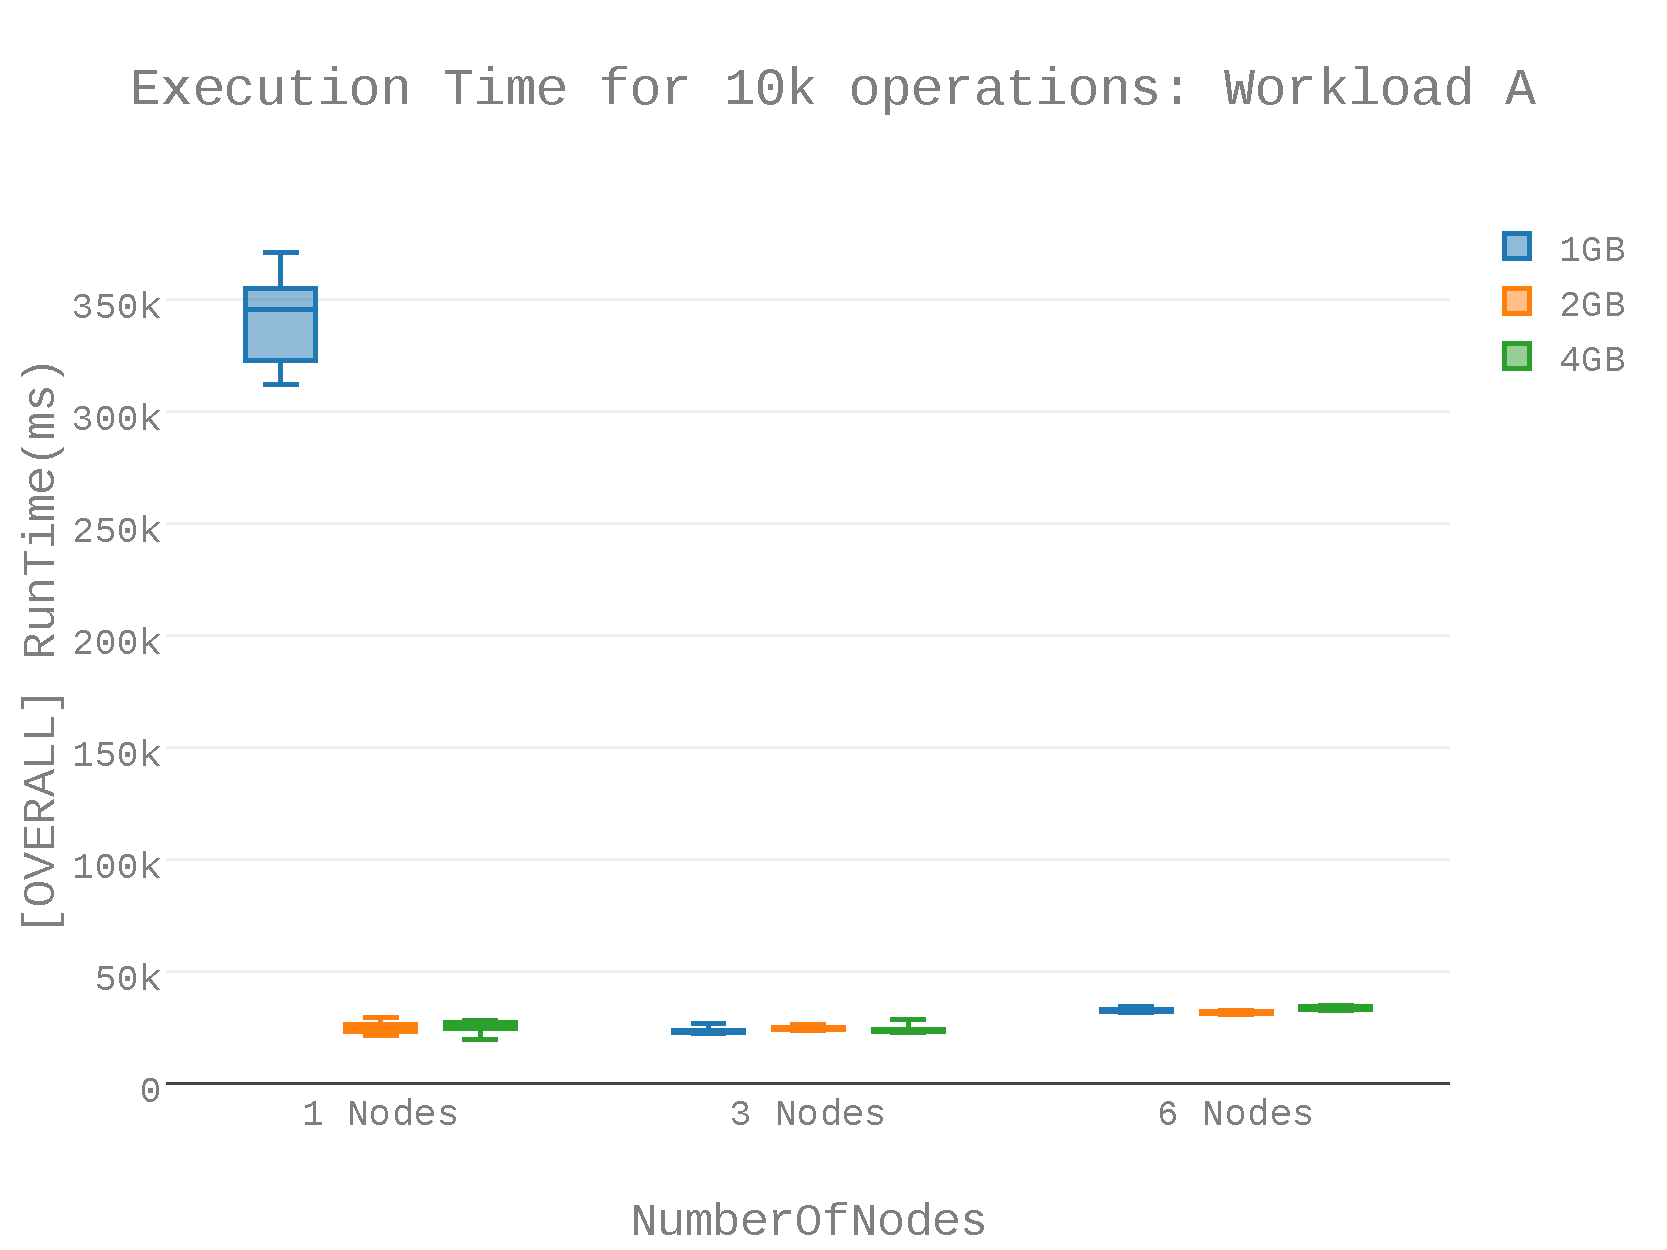
\includegraphics[width=3.5in]{Figures/figures-wle_fig4.pdf}

\caption{Execution time for virtual machines with 1GB, 2GB, and 4GB of \gls{ram}.  The first 9 trials have been removed in order to filter out the trials representing the cache effect and thus represent the steady state.}

\label{fig:figures-wle_fig4}
\end{figure}

\begin{table}
\begin{tabular}{lrrr}
\toprule
 index &  ram1GB &  ram2GB &  ram4GB \\
\midrule
 count &      21 &      21 &      21 \\
  mean &  356156 & 24989.5 & 25145.5 \\
   std & 6091.15 & 2157.15 &  2121.9 \\
   min &  347166 &   21164 &   19476 \\
   25\% &  350412 &   23254 &   24341 \\
   50\% &  354780 &   25159 &   25195 \\
   75\% &  360472 &   26145 &   26772 \\
   max &  371161 &   29166 &   27919 \\
 range &   23995 &    8002 &    8443 \\
\bottomrule
\end{tabular}
\caption{Summary Statistics for 1-Node Configuration. All values represented fall between 19476.0 ms and 371161.0 ms, or rather within a span of 351685.0 ms.}
\label{table:summary_statistics_for_1_config}
\end{table}
\begin{table}
\begin{tabular}{lrrr}
\toprule
 index &  ram1GB &  ram2GB &  ram4GB \\
\midrule
 count &      21 &      21 &      21 \\
  mean &   23444 & 24544.1 & 23753.2 \\
   std & 1016.02 & 747.466 & 1152.61 \\
   min &   22411 &   23430 &   22828 \\
   25\% &   22813 &   24169 &   23292 \\
   50\% &   23221 &   24399 &   23572 \\
   75\% &   23658 &   24662 &   23892 \\
   max &   26488 &   26396 &   28465 \\
 range &    4077 &    2966 &    5637 \\
\bottomrule
\end{tabular}
\caption{Summary Statistics for 3-Node Configuration. All values represented fall between 22411.0 ms and 28465.0 ms, or rather within a span of 6054.0 ms.}
\label{table:summary_statistics_for_3_config}
\end{table}
\begin{table}
\begin{tabular}{lrrr}
\toprule
 index &  ram1GB &  ram2GB &  ram4GB \\
\midrule
 count &      21 &      21 &      21 \\
  mean & 32493.2 & 31495.7 & 33605.4 \\
   std & 610.462 & 533.638 & 608.798 \\
   min &   31508 &   30551 &   32649 \\
   25\% &   32108 &   31081 &   33199 \\
   50\% &   32448 &   31466 &   33665 \\
   75\% &   32899 &   31896 &   34105 \\
   max &   34101 &   32522 &   34524 \\
 range &    2593 &    1971 &    1875 \\
\bottomrule
\end{tabular}
\caption{Summary Statistics for 6-Node Configuration. All values represented fall between 30551.0 ms and 34524.0 ms, or rather within a span of 3973.0 ms.}
\label{table:summary_statistics_for_6_config}
\end{table}

\paragraph{Absolute Ranges}

While Figure \ref{fig:figures-wle_fig4} gives a general sense of what the results look like, the actual summary statistics can be examined in Tables \ref{table:summary_statistics_for_1_config}, \ref{table:summary_statistics_for_3_config}, and \ref{table:summary_statistics_for_6_config}. After filtering out the first nine trials, the results for running 10,000 operations is displayed in Tables \ref{table:summary_statistics_for_1_config}, \ref{table:summary_statistics_for_3_config}, and \ref{table:summary_statistics_for_6_config}.  For each configuration, varying the \gls{ram} of the virtual machine resulted in execution times that fell within 2 seconds of each other.

\paragraph{\gls{anova}}

A one-way \gls{anova} was performed with the filtered data, and the \gls{anova} summary tables can be seen in Tables \ref{ram_variance_analysis_workload_a_1_node}, \ref{ram_variance_analysis_workload_a_3_node}, and \ref{ram_variance_analysis_workload_a_6_node} for the 1, 3, and 6 node cases respectively.  For each case, the  p-value is much, much less than 0.05, and thus it can be said that one can be 95\% confident in the decision to fail to reject the null hypothesis, the hypothesis that the means are equal.

\begin{table}
\begin{tabular}{lrrrrr}
\toprule
         Source &          SS &  df &          MS &       F &           p \\
\midrule
 between groups & 1.53468e+12 &   2 & 7.67339e+11 & 49764.9 & 2.50081e-97 \\
  within groups & 9.25156e+08 &  60 & 1.54193e+07 &     nan &         nan \\
          total &  1.5356e+12 &  62 &         nan &     nan &         nan \\
\bottomrule
\end{tabular}
\caption{ANOVA Summary Table for Workload E, 1 Node}
\label{table:ram_variance_analysis_workload_e_1_node}
\end{table}

\begin{table}
\begin{tabular}{lrrrrr}
\toprule
         Source &          SS &  df &          MS &       F &          p \\
\midrule
 between groups & 1.35194e+07 &   2 & 6.75969e+06 & 6.94605 & 0.00193463 \\
  within groups & 5.83902e+07 &  60 &      973170 &     nan &        nan \\
          total & 7.19096e+07 &  62 &         nan &     nan &        nan \\
\bottomrule
\end{tabular}
\caption{ANOVA Summary Table for Workload E, 3 Node}
\label{table:ram_variance_analysis_workload_e_3_node}
\end{table}

\begin{table}
\begin{tabular}{lrrrrr}
\toprule
         Source &          SS &  df &          MS &       F &          p \\
\midrule
 between groups & 4.67783e+07 &   2 & 2.33892e+07 & 68.2518 & 3.4948e-16 \\
  within groups & 2.05614e+07 &  60 &      342689 &     nan &        nan \\
          total & 6.73397e+07 &  62 &         nan &     nan &        nan \\
\bottomrule
\end{tabular}
\caption{ANOVA Summary Table for Workload E, 6 Node}
\label{table:ram_variance_analysis_workload_e_6_node}
\end{table}

Examining the effects of variance in the amount of \gls{ram} allocated the virtual machines does not seem to have a notable impact on performance.  This indicates that, any observed limitation on the Raspberry Pis’ performance is not limited by \gls{ram}, but something else, and that varying \gls{ram} in future tests will not yield significant results.

% Insert something about statistical significance

\subsection{Implementation on Raspberry Pi}

In a similar fashion, the tests were run on the Raspberry Pi to observe performance.  The spread of each of the tests can be seen in Figure \ref{fig:wle_fig10} and Table \ref{table:wired-results}.  The results, next to one trend for the virtual machines, can be seen in Figure \ref{fig:fig06}. 

\begin{figure}[h]
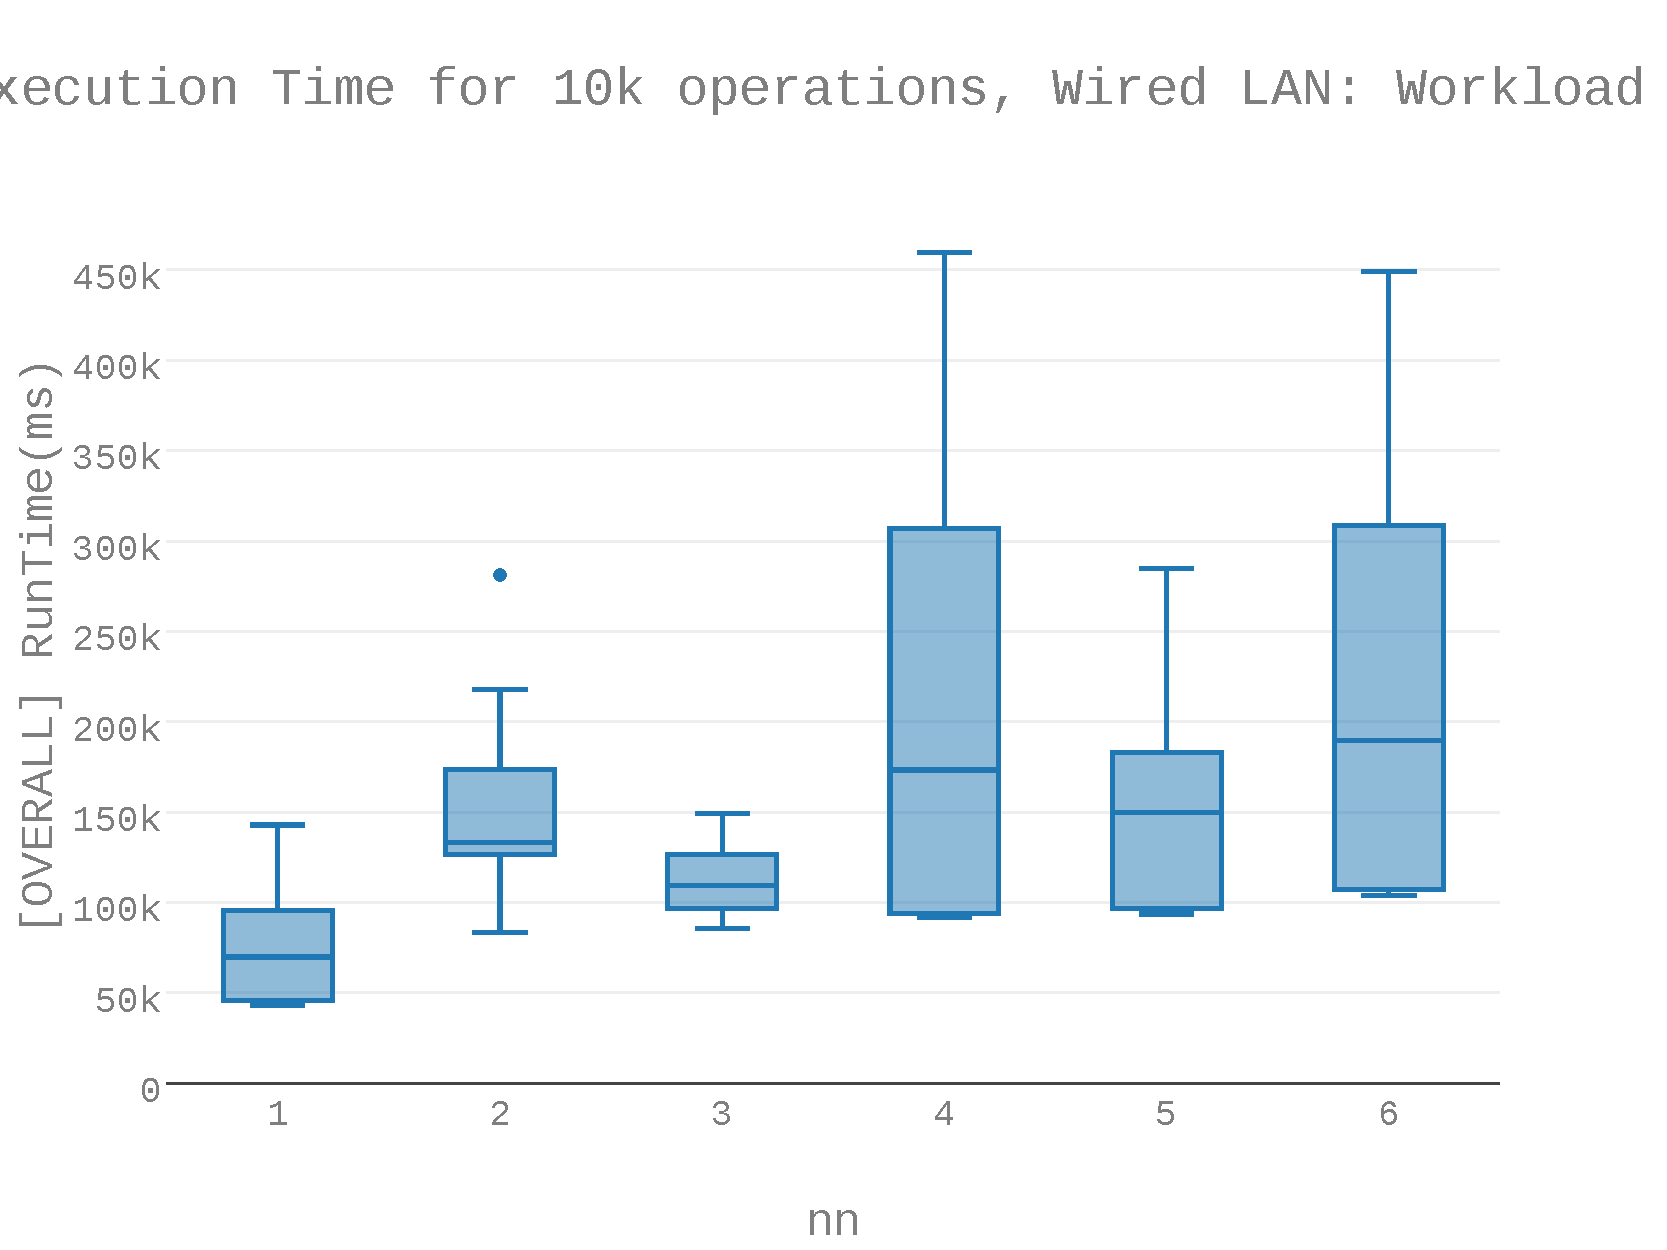
\includegraphics[width=3.5in]{Figures/figures-wle_fig10.pdf}

\caption{Box plot representing the results of the workload applied to wired local area network on the Raspberry Pi platform.}

\label{fig:wle_fig10}
\end{figure}

\begin{figure}[h]
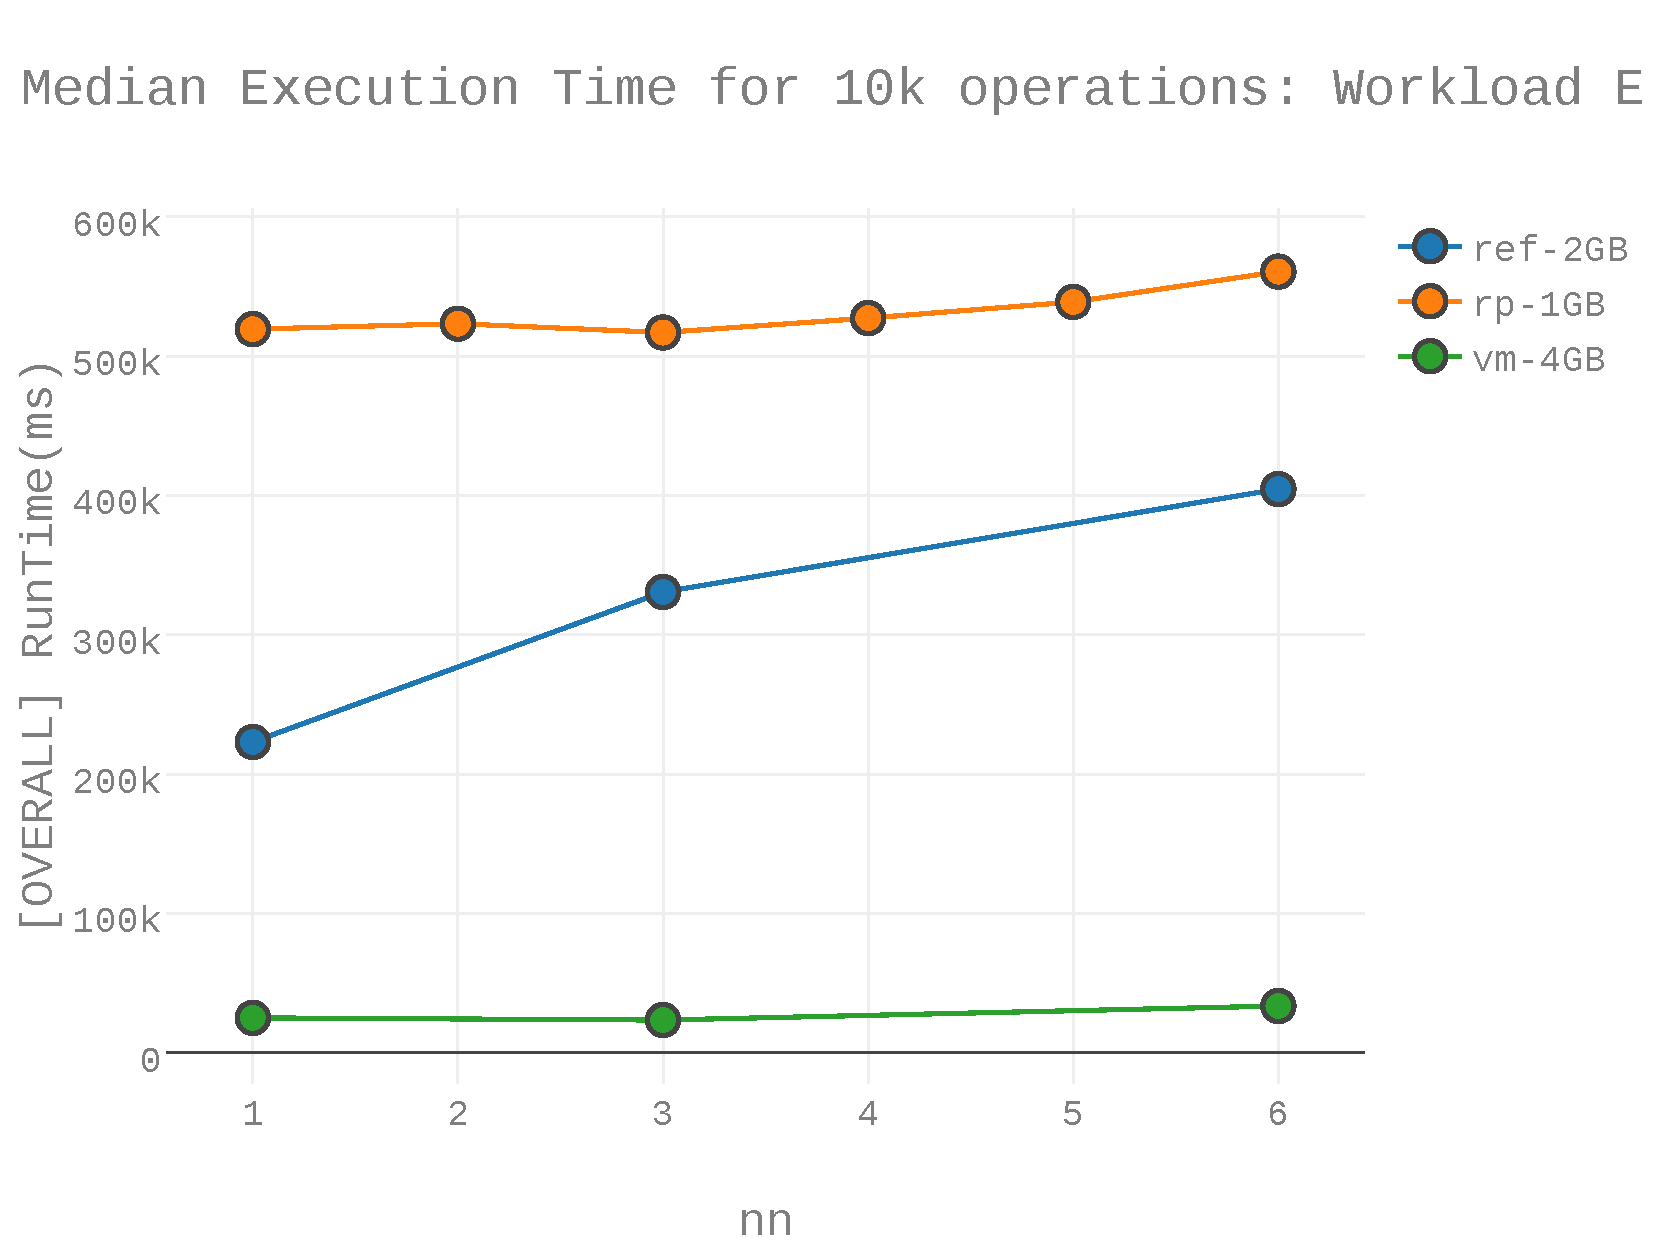
\includegraphics[width=3.5in]{Figures/figures-wle_fig6.pdf}

\caption{Comparison between the Raspberry Pi nodes (rp-1GB), the results reported in \cite{Abramova2014} (ref-2GB), and the virtual nodes with 4GB available \gls{ram} (vm-4GB).}

\label{fig:fig06}
\end{figure}

\begin{table}
\begin{tabular}{lrrr}
\toprule
 index &       1 &       3 &       6 \\
\midrule
 count &      21 &      21 &      21 \\
  mean & 5.2e+05 & 5.2e+05 & 5.6e+05 \\
   std & 2.1e+03 & 5.5e+03 &   3e+03 \\
   min & 5.2e+05 & 5.1e+05 & 5.6e+05 \\
   25\% & 5.2e+05 & 5.1e+05 & 5.6e+05 \\
   50\% & 5.2e+05 & 5.2e+05 & 5.6e+05 \\
   75\% & 5.2e+05 & 5.2e+05 & 5.6e+05 \\
   max & 5.2e+05 & 5.3e+05 & 5.7e+05 \\
 range & 8.3e+03 &   2e+04 &   1e+04 \\
\bottomrule
\end{tabular}
\caption{Summary for Raspberry Pi wired local area network}
\label{table:rp_wired_summary_statistics}
\end{table}

As can be seen from Figure \ref{fig:fig06}, the Raspberry Pi configuration takes considerably more execution time than the virtual machine analogy, which is probably due to the physical nature of the Ethernet connections (propagation delay) and the I/O limitations of the Raspberry Pi hardware.  However, its seemingly similar performance to the reference in \cite{Abramova2014} suggests the \gls{io} for the \gls{sd} Card follows a predictable pattern, and actually seems to outperform the node in \cite{Abramova2014} in the degenerate 1-node case.

For this paragraph, consider the results from \cite{Abramova2014} as the reference.  For a node network of 1, the experimental values fell between 515941.0 ms and 524199.0 ms, inclusive, and all values fell within 301019.0 ms of the reference value of 223180 ms.  For a node network of 3, the experimental values fell between 511997.0 ms and 532260.0 ms, inclusive, and all values fell within 201440.0 ms of the reference value of 330820 ms.  For a node network of 6, the experimental values fell between 555007.0 ms and 565388.0 ms, inclusive, and all values fell within 160728.0 ms of the reference value of 404660 ms.  

\subsection{Wireless Links}

The median value of the corresponding wired experiment will serve as the reference in this paragraph. For a node network of 1, the experimental values fell between 625938.0 ms and 724603.0 ms, inclusive, and all values fell within 204854.0 ms of the reference value of 519749.0 ms.  For a node network of 3, the experimental values fell between 1198600.0 ms and 1458086.0 ms, inclusive, and all values fell within 941493.0 ms of the reference value of 516593.0 ms.  For a node network of 6, the experimental values fell between 260.0 ms and 2018342.0 ms, inclusive, and all values fell within 1459859.0 ms of the reference value of 558483.0 ms.  

\begin{figure}[h]
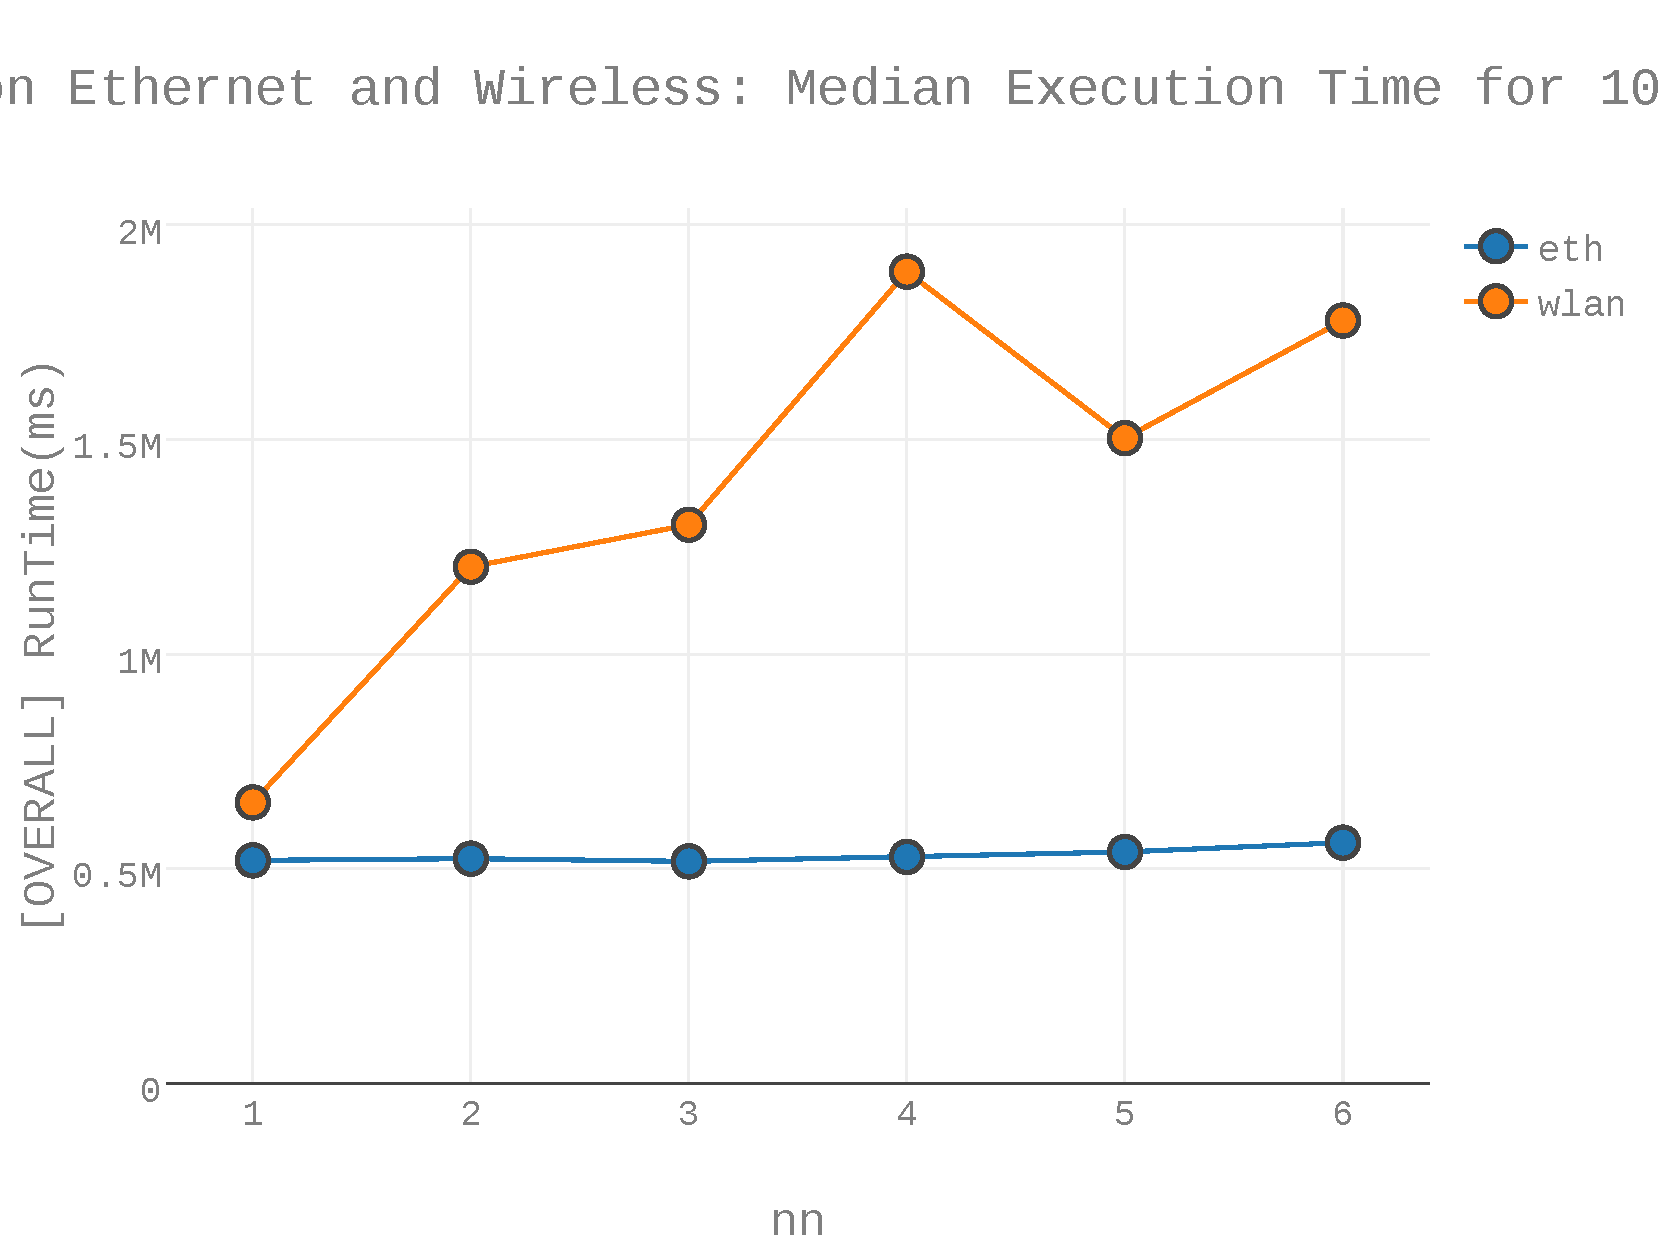
\includegraphics[width=3.5in]{Figures/figures-wle_fig7.pdf}

\caption{Comparison between the Ethernet links (eth) and wireless links (wlan) using the Raspberry Pi nodes.}

\label{fig:fig07}
\end{figure}

Figure \ref{fig:fig07} depicts the two experiments using Raspberry Pis: a wireless LAN (wlan) and an Ethernet LAN (eth).  In Figure \ref{fig:fig07}, as well as previous graphs, one can observe that the the Ethernet LAN effects about 50 seconds of execution time for 10,000 operations.  The initial median execution time for a node on a wireless LAN was found to be double the execution time.

For both configurations, performance takes a hit when transitioning from 1 to 2 nodes, but then increases from 2 nodes to 3 nodes.  From 3 nodes to 4 nodes, the wireless LAN configuration’s performance decreases dramatically, compared to slight increase in the wired Ethernet case.  

\begin{figure}[h]
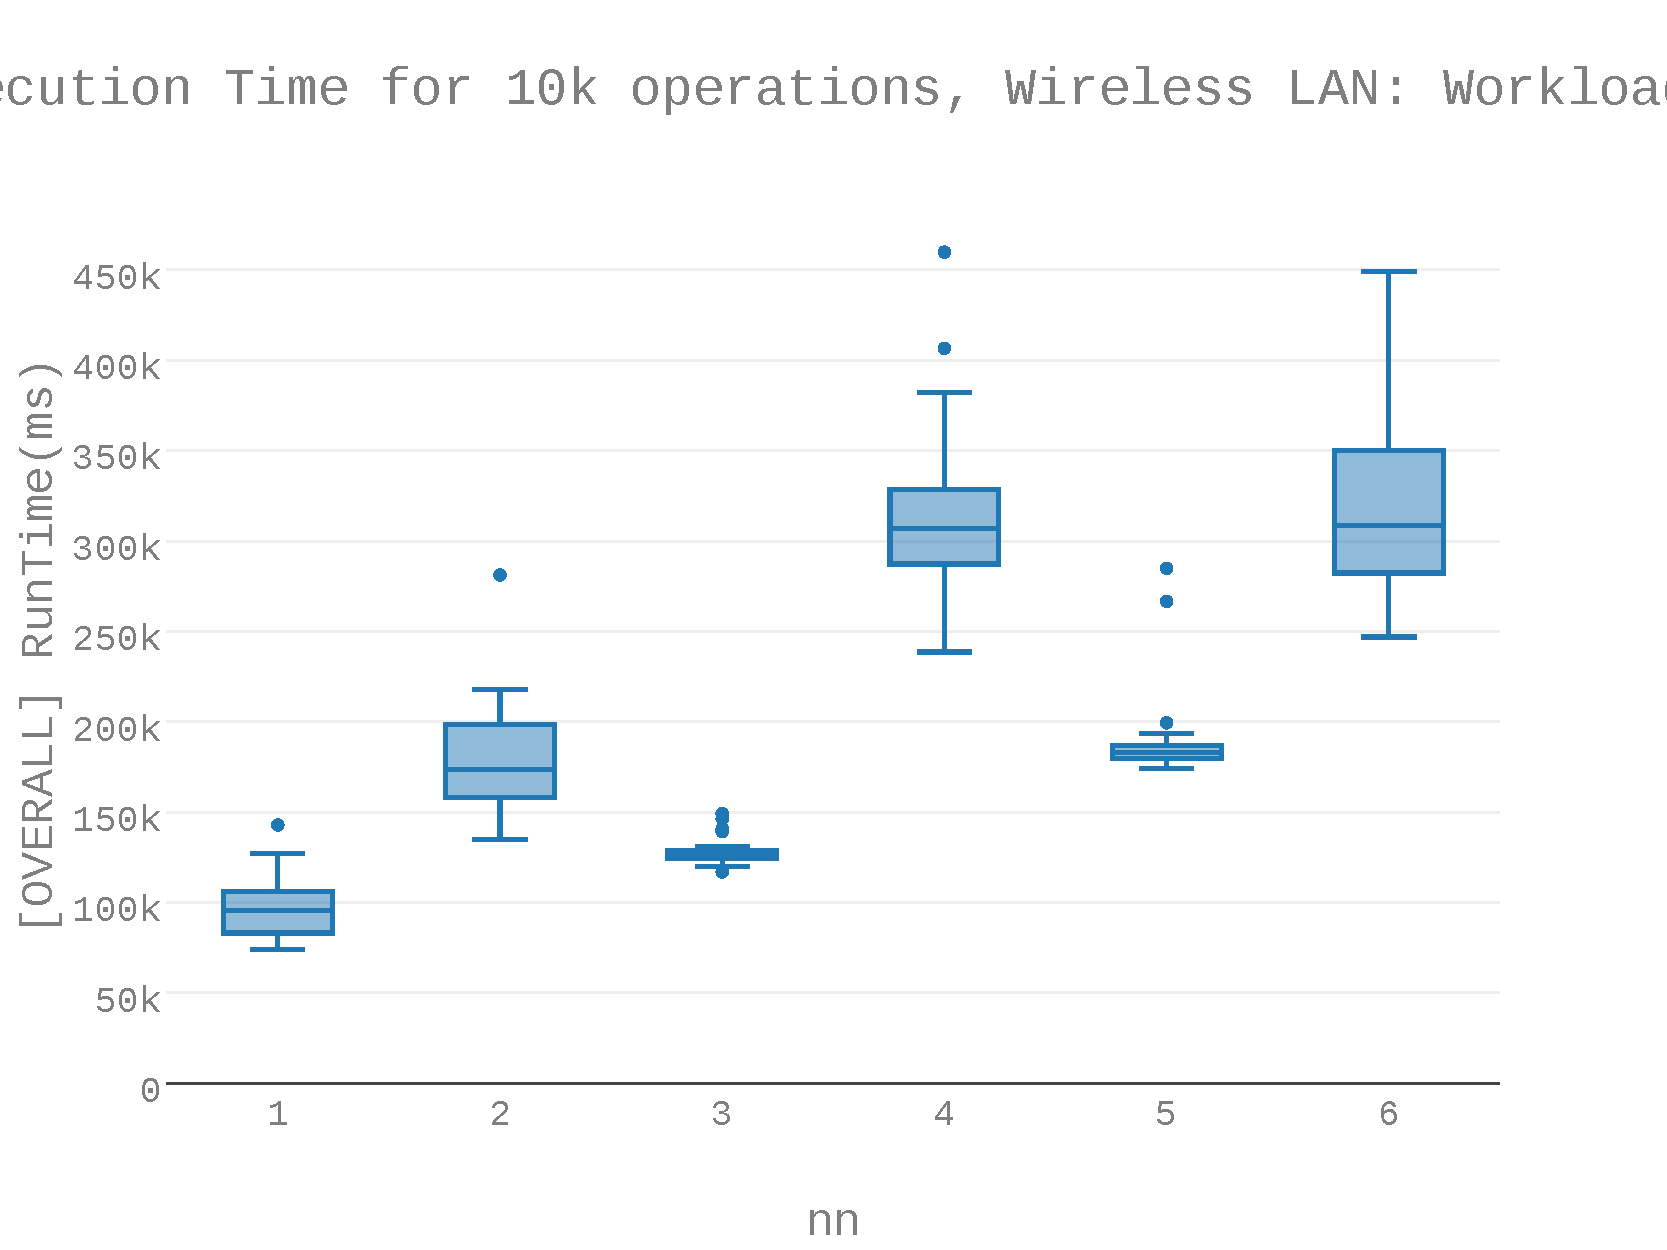
\includegraphics[width=3.5in]{Figures/figures-wle_fig8.pdf}

\caption{Distribution for all 30 trials of execution times where the Raspberry Pi nodes were connected via a wireless \gls{lan}.  Suspected outliers, values more than 3 times the interquartile range, are included as individual points above and below the 'maximum' and 'minimum' bars.}

\label{fig:fig08}
\end{figure}

A summary representation box plot of the results of wireless experimentation is above.  Here, the laptop was connected to the router via an Ethernet cable, and each node was connected to the router on a wireless local area network (LAN).  Suspected outliers, values more than 3 times the interquartile range (IQR) are included as points above and below.
There seems to be an overall increasing trend, while the data seems to oscillate, performing better for odd (1,3,5 node) configurations than for even (2,4,6 node) configurations.  However, there is no current theory behind this anomaly. 

\begin{figure}[h]
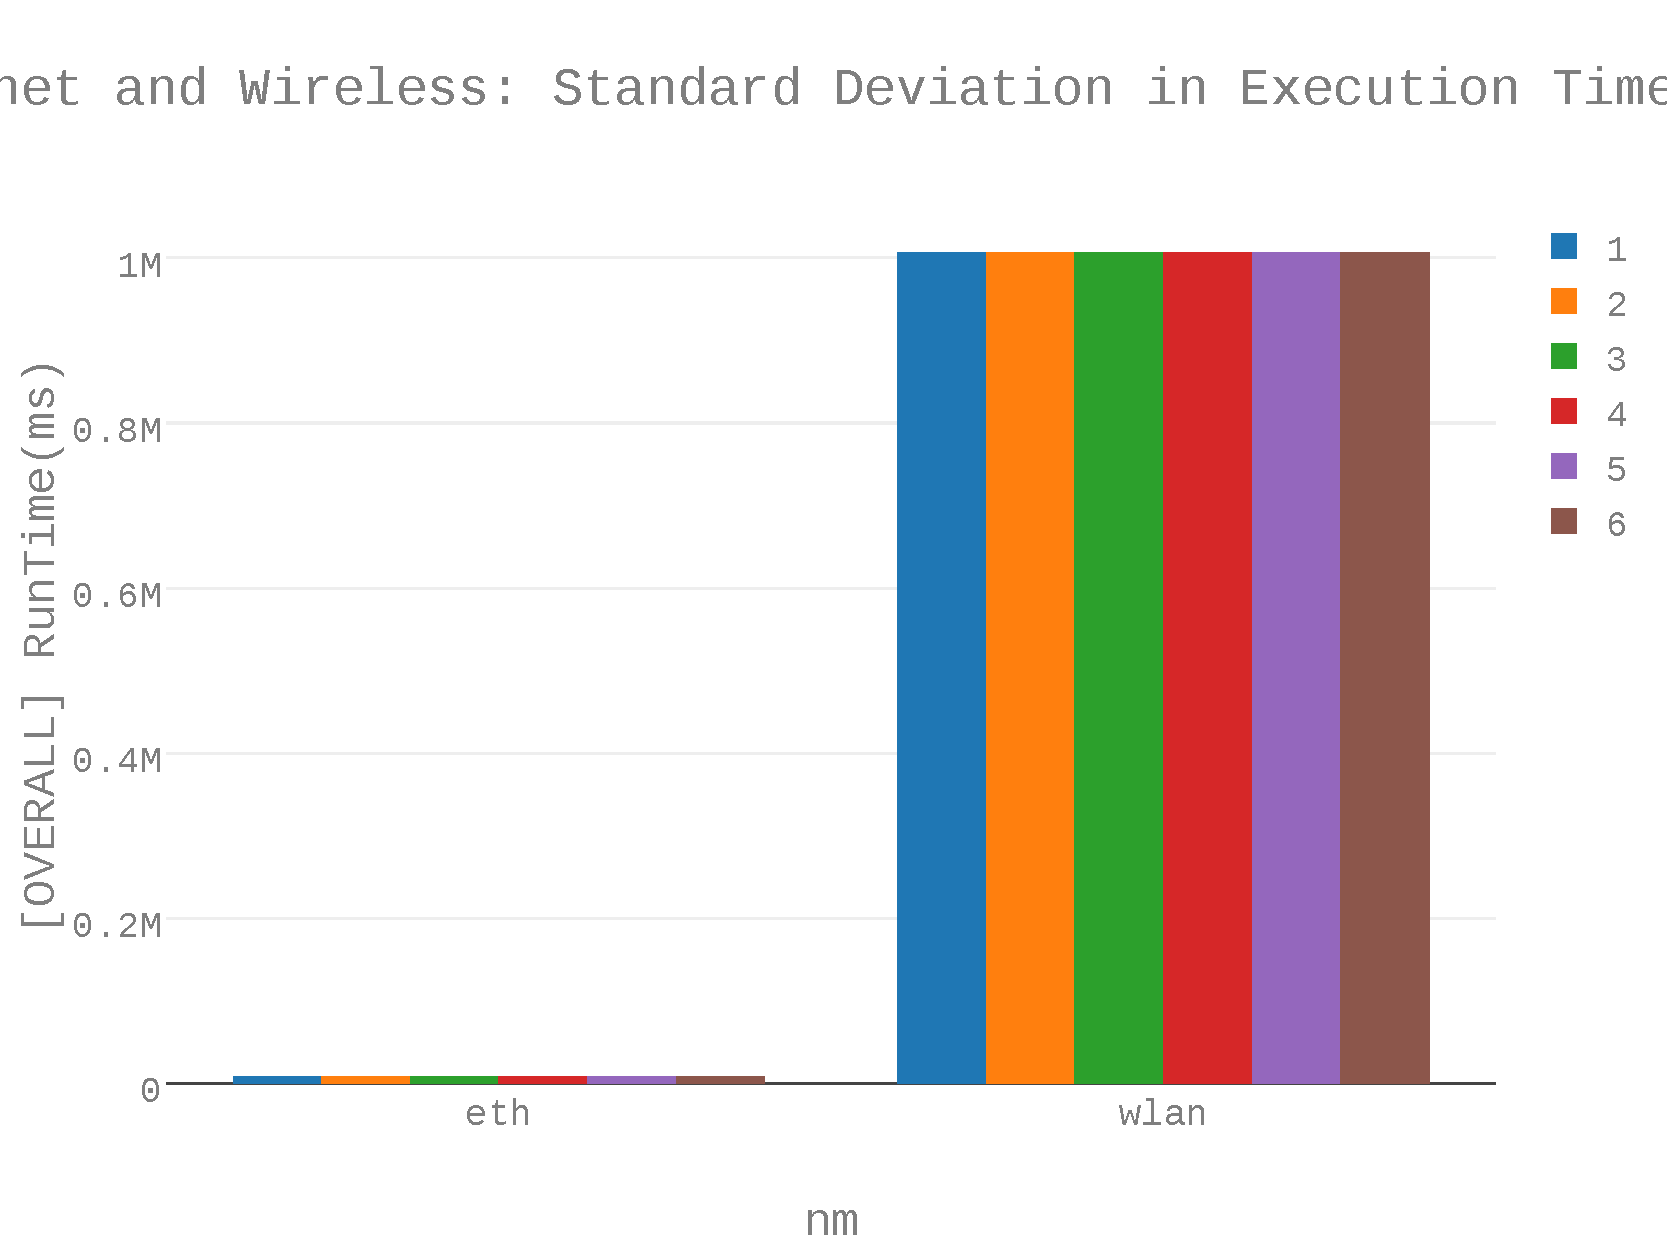
\includegraphics[width=3.5in]{Figures/figures-wle_fig9.pdf}

\caption{This compares the standard deviation in execution times for 10,000 operations of Workload C on the wired (eth) versus the wireless (wlan) configurations for 1 node, 2 nodes, 3 nodes, up through 6 nodes in milliseconds.}

\label{fig:fig09}
\end{figure}

To supplement the box plot, the standard deviation execution times for each set of trials, separated by number of nodes, is depicted in Figure \ref{fig:fig09}.  The difference seen here appears stark, and is overwhelming compared to the variance between 1, 2, 3, 4, 5 and 6 node networks given the same communication method. 

%1)      Reduced performance of Workload A is not statistically significant for the reduced memory sizes of IoT like devices
%2)      When varying platforms, performance for Workload A tracks the performance of the reference paper. For trials performe, reduced performance of Workload A is within 100ms of the reference paper (abramova) for wired implementations.
%3)      When varying communication method, reduced performance of Workload A is within 100ms of the wired platform test (order of magnitude, no greater than 100% increase in delay)
%4)      Reduced performance of Workload C is not statistically significant for the reduced memory sizes of IoT like devices
%5)      When varying platforms, reduced performance of Workload C is within 100ms of the reference paper (abramova) for wired implementations
%6)      When varying communication method, reduced performance of Workload C is within 100ms of the wired platform test
%7)      Reduced performance of Workload E is not statistically significant for the reduced memory sizes of IoT like devices
%8)      When varying platforms, reduced performance of Workload E is within 100ms of the reference paper (abramova) for wired implementations
%9)      When varying communication method, reduced performance of Workload E is within 100ms of the wired platform test

%\section{Results - Research Question 4}

\subsection{Comparing Existing Work: VM vs REF}

\subsubsection{Initial Observations}

\subsubsection{Ordinal Statistics}

\subsubsection{Speedup Analysis}

Since this is a custom benchmark, there exists no readily available comparison with which one can compare execution times.

\subsection{1GB RAM vs 2GB RAM vs 4GB RAM}

We now discuss testing and performance for memory sizes ranging from 1GB to 4GB.  The experience with 512MB was documented with Workload A.

This section describes the results of running the \gls{ycsb} on virtual node networks as described in the methodology.  The summary of execution times are reported in Tables \ref{table:summary_statistics_for_1_config}, \ref{table:summary_statistics_for_3_config}, and \ref{table:summary_statistics_for_6_config}.  For each table, the summary statistics are listed for each amount of memory.

\subsubsection{Initial Observations}

%--fig4--%

It is best to start with a visual inspection of the data represented in Figure \ref{fig:figures-wli_fig4}.  Generally the greater amount of \gls{ram}, the fewer problems one would have with memory overloads, or needing to compact. However, for each sample, it seems that different amount of memory yields the best performance.

By all appearances, it does seem that the 4GB of RAM outperforms the 1GB of RAM and the 2GB of RAM in this case.  It appears that for the 1-node degenerate case, the means could be about equal.  However, for 2, 3, 4, 5, and 6-node clusters, the 4GB seems to have an advantage in the samples here, both in terms of the overall performance in execution time but the deviation from the median as well.

It is not clear from this graph what accounts for the differences.  One possible explanation is compaction: the 4GB nodes never really need to compact.  The amount of data becomes too much for the 1GB and 2GB nodes to hold in the memtables in memory without doing a compaction, and thus allocates, on average, more resources for the triggered compaction events to flush the memtables and get the data onto disk.  To verify this, one could manually inspect sniffed data and/or log compaction events to measure any correlation among memtable size, partition size, node count in the cluster, and frequency of compaction events.  However, if this were the only factor, one would expect to see a particular pattern as the number of nodes in the cluster increased while the number of operations were constant:  low variance from frequent compaction, high variance from periodic compaction, and finally low variance from seldom or nonexistant compaction.  If this is indeed a significant factor, this might be ameliorated by increasing the number of operations, right now set at 10,000, to 100,000 to better represent the steady state.


\begin{figure}[h]
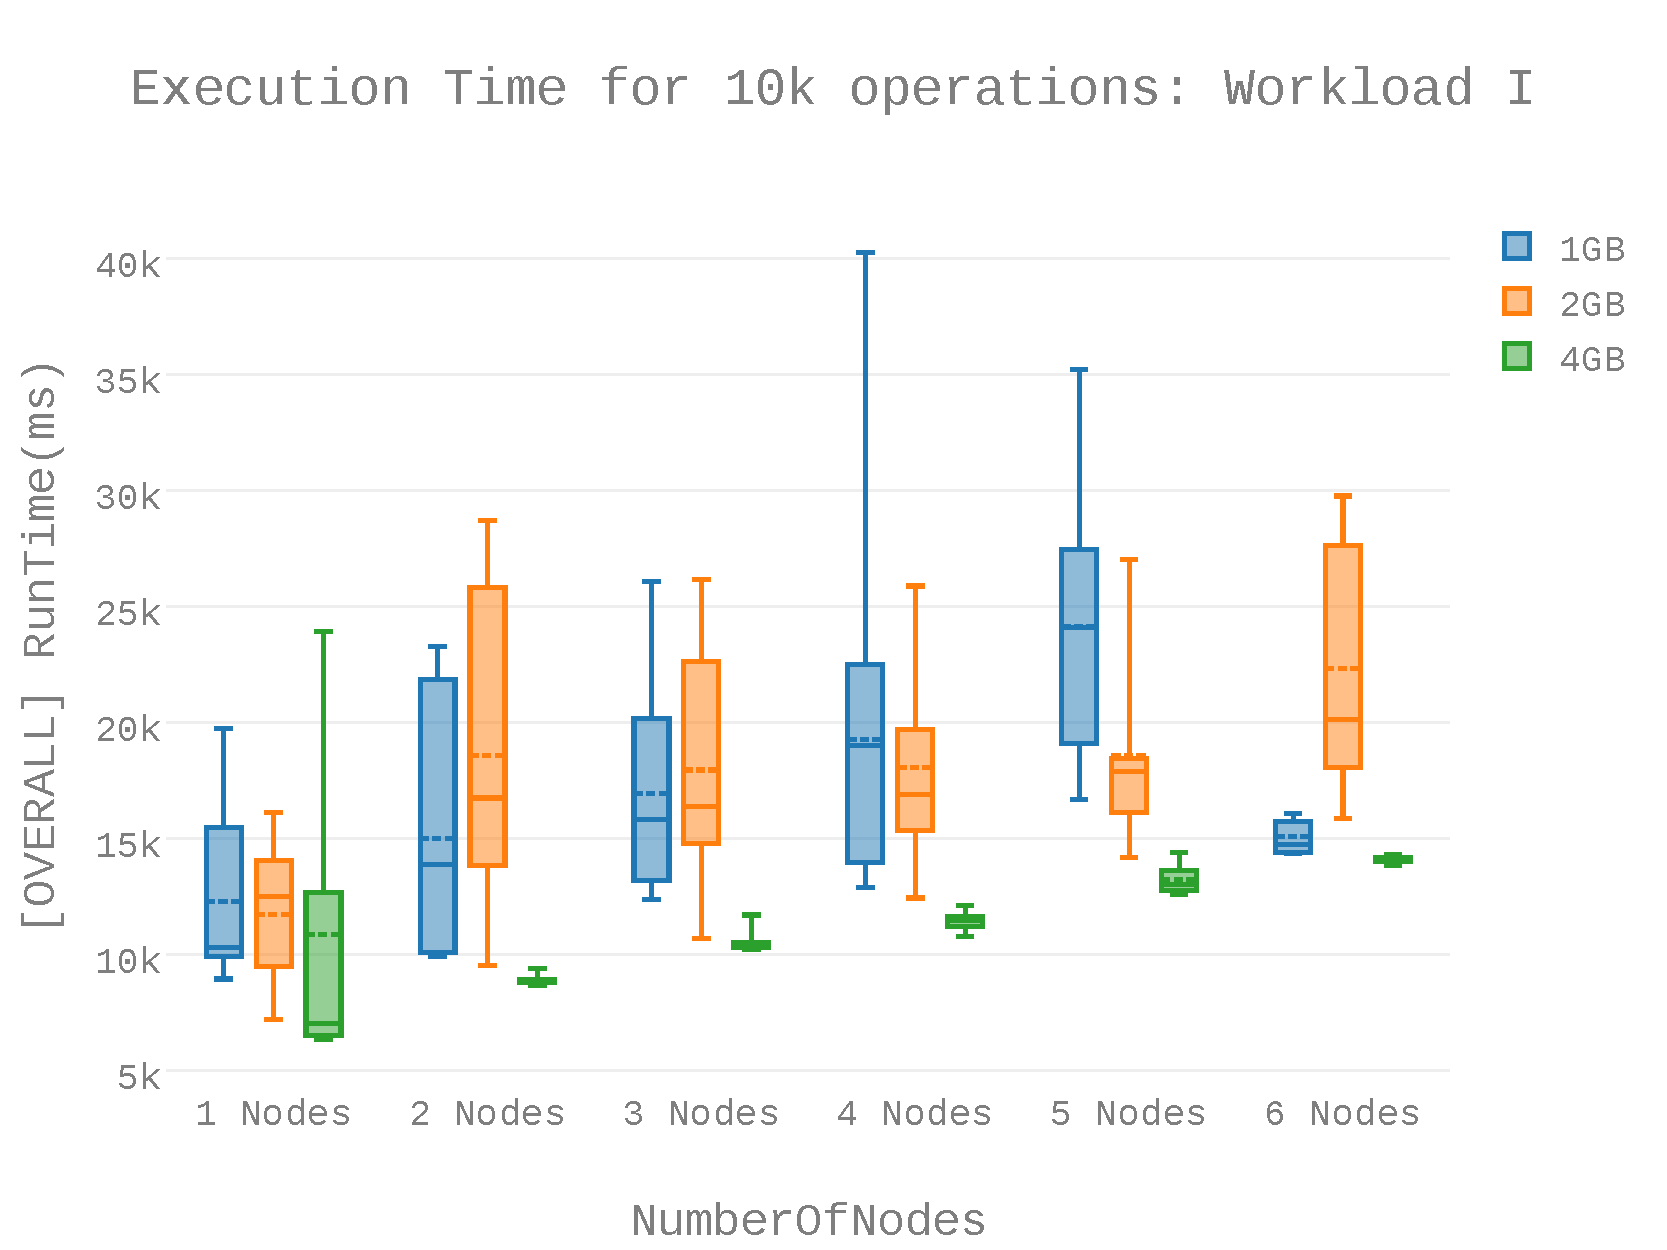
\includegraphics[width=7in]{Figures/figures-wli_fig4.pdf}

\caption{Execution time for virtual machines with 1GB, 2GB, and 4GB of \gls{ram}.  The first 9 trials have been removed in order to filter out the trials representing the cache effect and thus represent the steady state.}

\label{fig:figures-wli_fig4}
\end{figure}

\begin{table}
\begin{tabular}{lrrr}
\toprule
 index &  ram1GB &  ram2GB &  ram4GB \\
\midrule
 count &      21 &      21 &      21 \\
  mean &  356156 & 24989.5 & 25145.5 \\
   std & 6091.15 & 2157.15 &  2121.9 \\
   min &  347166 &   21164 &   19476 \\
   25\% &  350412 &   23254 &   24341 \\
   50\% &  354780 &   25159 &   25195 \\
   75\% &  360472 &   26145 &   26772 \\
   max &  371161 &   29166 &   27919 \\
 range &   23995 &    8002 &    8443 \\
\bottomrule
\end{tabular}
\caption{Summary Statistics for 1-Node Configuration. All values represented fall between 19476.0 ms and 371161.0 ms, or rather within a span of 351685.0 ms.}
\label{table:summary_statistics_for_1_config}
\end{table}
\begin{table}
\begin{tabular}{lrrr}
\toprule
 index &  ram1GB &  ram2GB &  ram4GB \\
\midrule
 count &      21 &      21 &      21 \\
  mean &   23444 & 24544.1 & 23753.2 \\
   std & 1016.02 & 747.466 & 1152.61 \\
   min &   22411 &   23430 &   22828 \\
   25\% &   22813 &   24169 &   23292 \\
   50\% &   23221 &   24399 &   23572 \\
   75\% &   23658 &   24662 &   23892 \\
   max &   26488 &   26396 &   28465 \\
 range &    4077 &    2966 &    5637 \\
\bottomrule
\end{tabular}
\caption{Summary Statistics for 3-Node Configuration. All values represented fall between 22411.0 ms and 28465.0 ms, or rather within a span of 6054.0 ms.}
\label{table:summary_statistics_for_3_config}
\end{table}
\begin{table}
\begin{tabular}{lrrr}
\toprule
 index &  ram1GB &  ram2GB &  ram4GB \\
\midrule
 count &      21 &      21 &      21 \\
  mean & 32493.2 & 31495.7 & 33605.4 \\
   std & 610.462 & 533.638 & 608.798 \\
   min &   31508 &   30551 &   32649 \\
   25\% &   32108 &   31081 &   33199 \\
   50\% &   32448 &   31466 &   33665 \\
   75\% &   32899 &   31896 &   34105 \\
   max &   34101 &   32522 &   34524 \\
 range &    2593 &    1971 &    1875 \\
\bottomrule
\end{tabular}
\caption{Summary Statistics for 6-Node Configuration. All values represented fall between 30551.0 ms and 34524.0 ms, or rather within a span of 3973.0 ms.}
\label{table:summary_statistics_for_6_config}
\end{table}

\subsubsection{Ordinal Statistics}

While Figure \ref{fig:figures-wle_fig4} gives a general sense of what the results look like, the actual summary statistics can be examined in Tables \ref{table:summary_statistics_for_1_config}, \ref{table:summary_statistics_for_3_config}, and \ref{table:summary_statistics_for_6_config}. After filtering out the first nine trials, the results for running 10,000 operations is displayed in Tables \ref{table:summary_statistics_for_1_config}, \ref{table:summary_statistics_for_3_config}, and \ref{table:summary_statistics_for_6_config}.  For each configuration, varying the \gls{ram} of the virtual machine resulted in execution times that fell within 2 seconds of each other.

\subsubsection{Linear Regression for Each Node Cluster Size}

\paragraph{1-Node Cluster}
\paragraph{2-Node Cluster}
\paragraph{3-Node Cluster}
\paragraph{4-Node Cluster}
\paragraph{5-Node Cluster}
\paragraph{6-Node Cluster}

A one-way \gls{anova} was performed with the filtered data, and the \gls{anova} summary tables can be seen in Tables \ref{ram_variance_analysis_workload_a_1_node}, \ref{ram_variance_analysis_workload_a_3_node}, and \ref{ram_variance_analysis_workload_a_6_node} for the 1, 3, and 6 node cases respectively.  For each case, the  p-value is much, much less than 0.05, and thus it can be said that one can be 95\% confident in the decision to fail to reject the null hypothesis, the hypothesis that the means are equal.

\begin{table}
\begin{tabular}{lrrrrr}
\toprule
         Source &          SS &  df &          MS &       F &           p \\
\midrule
 between groups & 1.53468e+12 &   2 & 7.67339e+11 & 49764.9 & 2.50081e-97 \\
  within groups & 9.25156e+08 &  60 & 1.54193e+07 &     nan &         nan \\
          total &  1.5356e+12 &  62 &         nan &     nan &         nan \\
\bottomrule
\end{tabular}
\caption{ANOVA Summary Table for Workload E, 1 Node}
\label{table:ram_variance_analysis_workload_e_1_node}
\end{table}

\begin{table}
\begin{tabular}{lrrrrr}
\toprule
         Source &          SS &  df &          MS &       F &          p \\
\midrule
 between groups & 1.35194e+07 &   2 & 6.75969e+06 & 6.94605 & 0.00193463 \\
  within groups & 5.83902e+07 &  60 &      973170 &     nan &        nan \\
          total & 7.19096e+07 &  62 &         nan &     nan &        nan \\
\bottomrule
\end{tabular}
\caption{ANOVA Summary Table for Workload E, 3 Node}
\label{table:ram_variance_analysis_workload_e_3_node}
\end{table}

\begin{table}
\begin{tabular}{lrrrrr}
\toprule
         Source &          SS &  df &          MS &       F &          p \\
\midrule
 between groups & 4.67783e+07 &   2 & 2.33892e+07 & 68.2518 & 3.4948e-16 \\
  within groups & 2.05614e+07 &  60 &      342689 &     nan &        nan \\
          total & 6.73397e+07 &  62 &         nan &     nan &        nan \\
\bottomrule
\end{tabular}
\caption{ANOVA Summary Table for Workload E, 6 Node}
\label{table:ram_variance_analysis_workload_e_6_node}
\end{table}

Examining the effects of variance in the amount of \gls{ram} allocated the virtual machines does not seem to have a notable impact on performance.  This indicates that, any observed limitation on the Raspberry Pis’ performance is not limited by \gls{ram}, but something else, and that varying \gls{ram} in future tests will not yield significant results.

% Insert something about statistical significance

\subsection{Implementation on Raspberry Pi}

\subsubsection{Initial Observations}

\subsubsection{Ordinal Statistics}

\subsubsection{Scalability of Node Cluster Size}

In a similar fashion, the tests were run on the Raspberry Pi to observe performance.  The spread of each of the tests can be seen in Figure \ref{fig:wle_fig10} and Table \ref{table:wired-results}.  The results, next to one trend for the virtual machines, can be seen in Figure \ref{fig:fig06}. 

\begin{figure}[h]
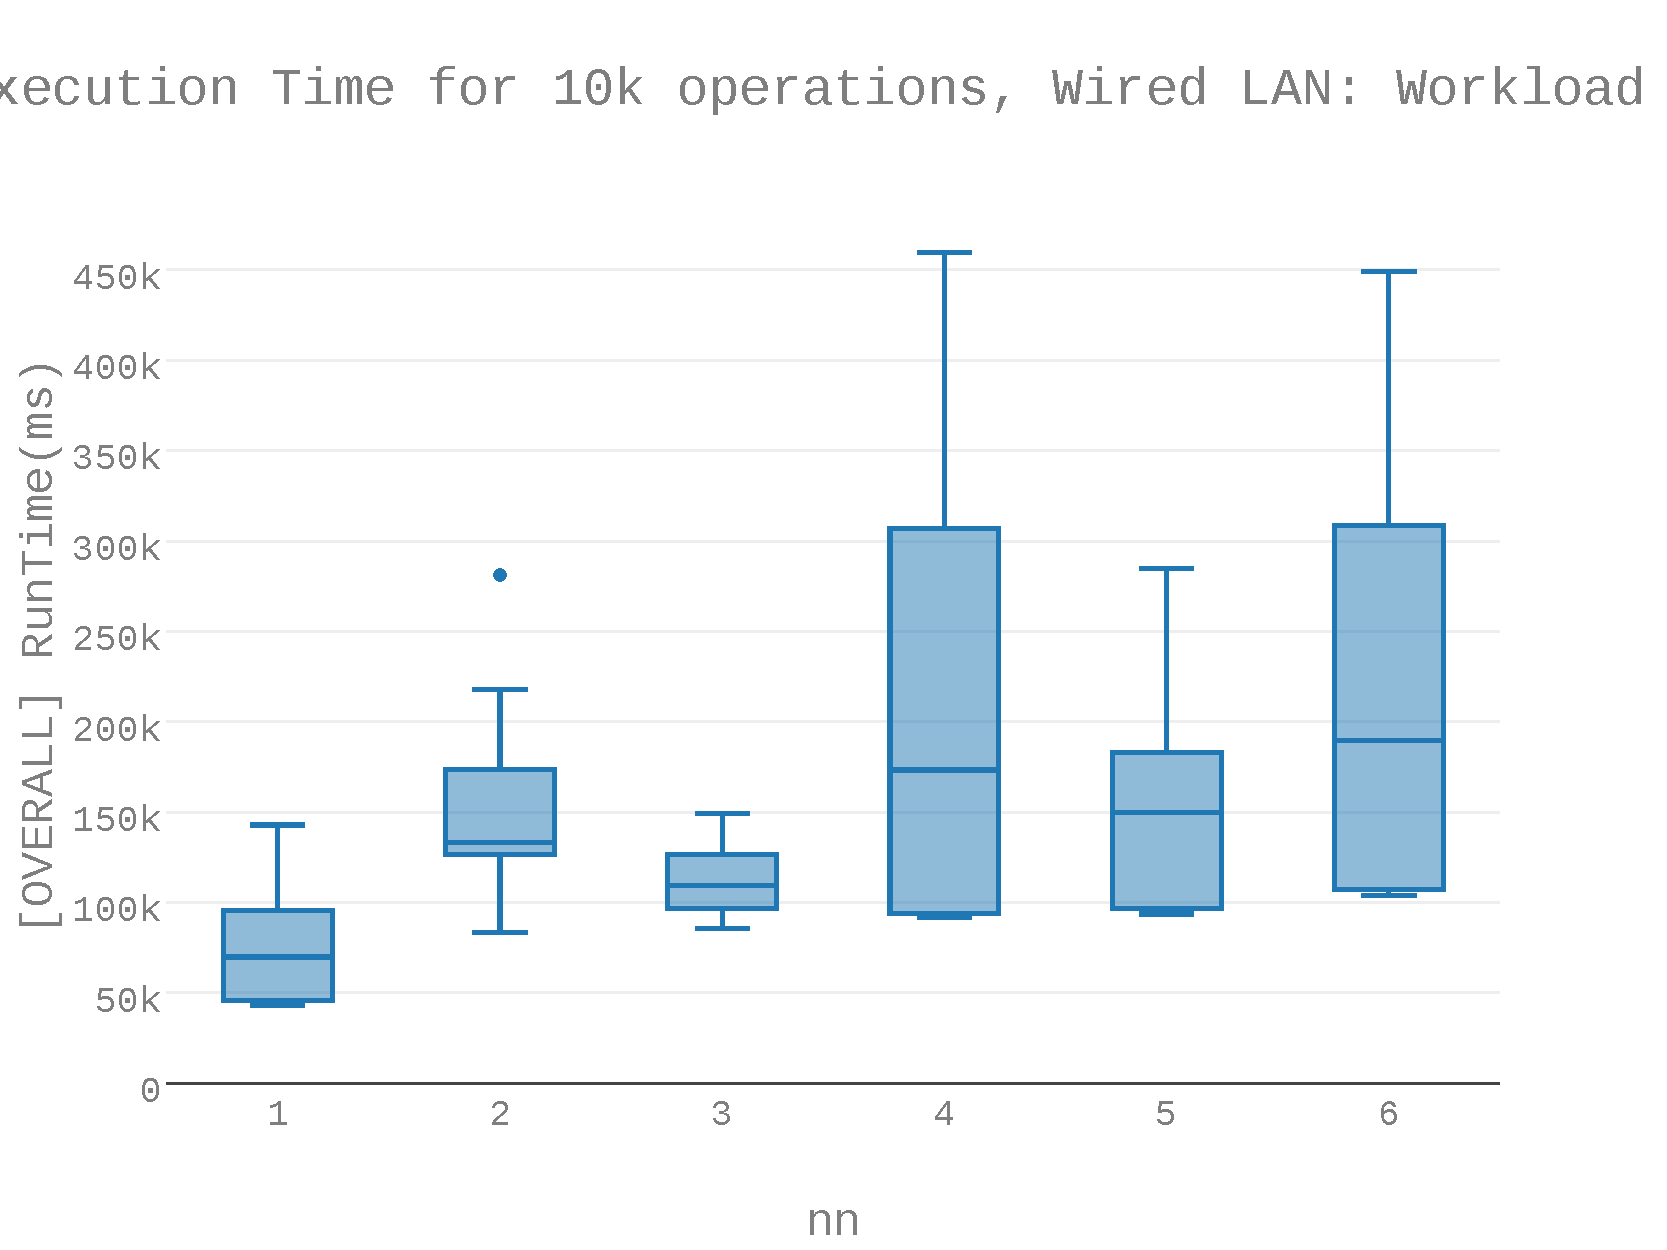
\includegraphics[width=3.5in]{Figures/figures-wle_fig10.pdf}

\caption{Box plot representing the results of the workload applied to wired local area network on the Raspberry Pi platform.}

\label{fig:wle_fig10}
\end{figure}

\begin{figure}[h]
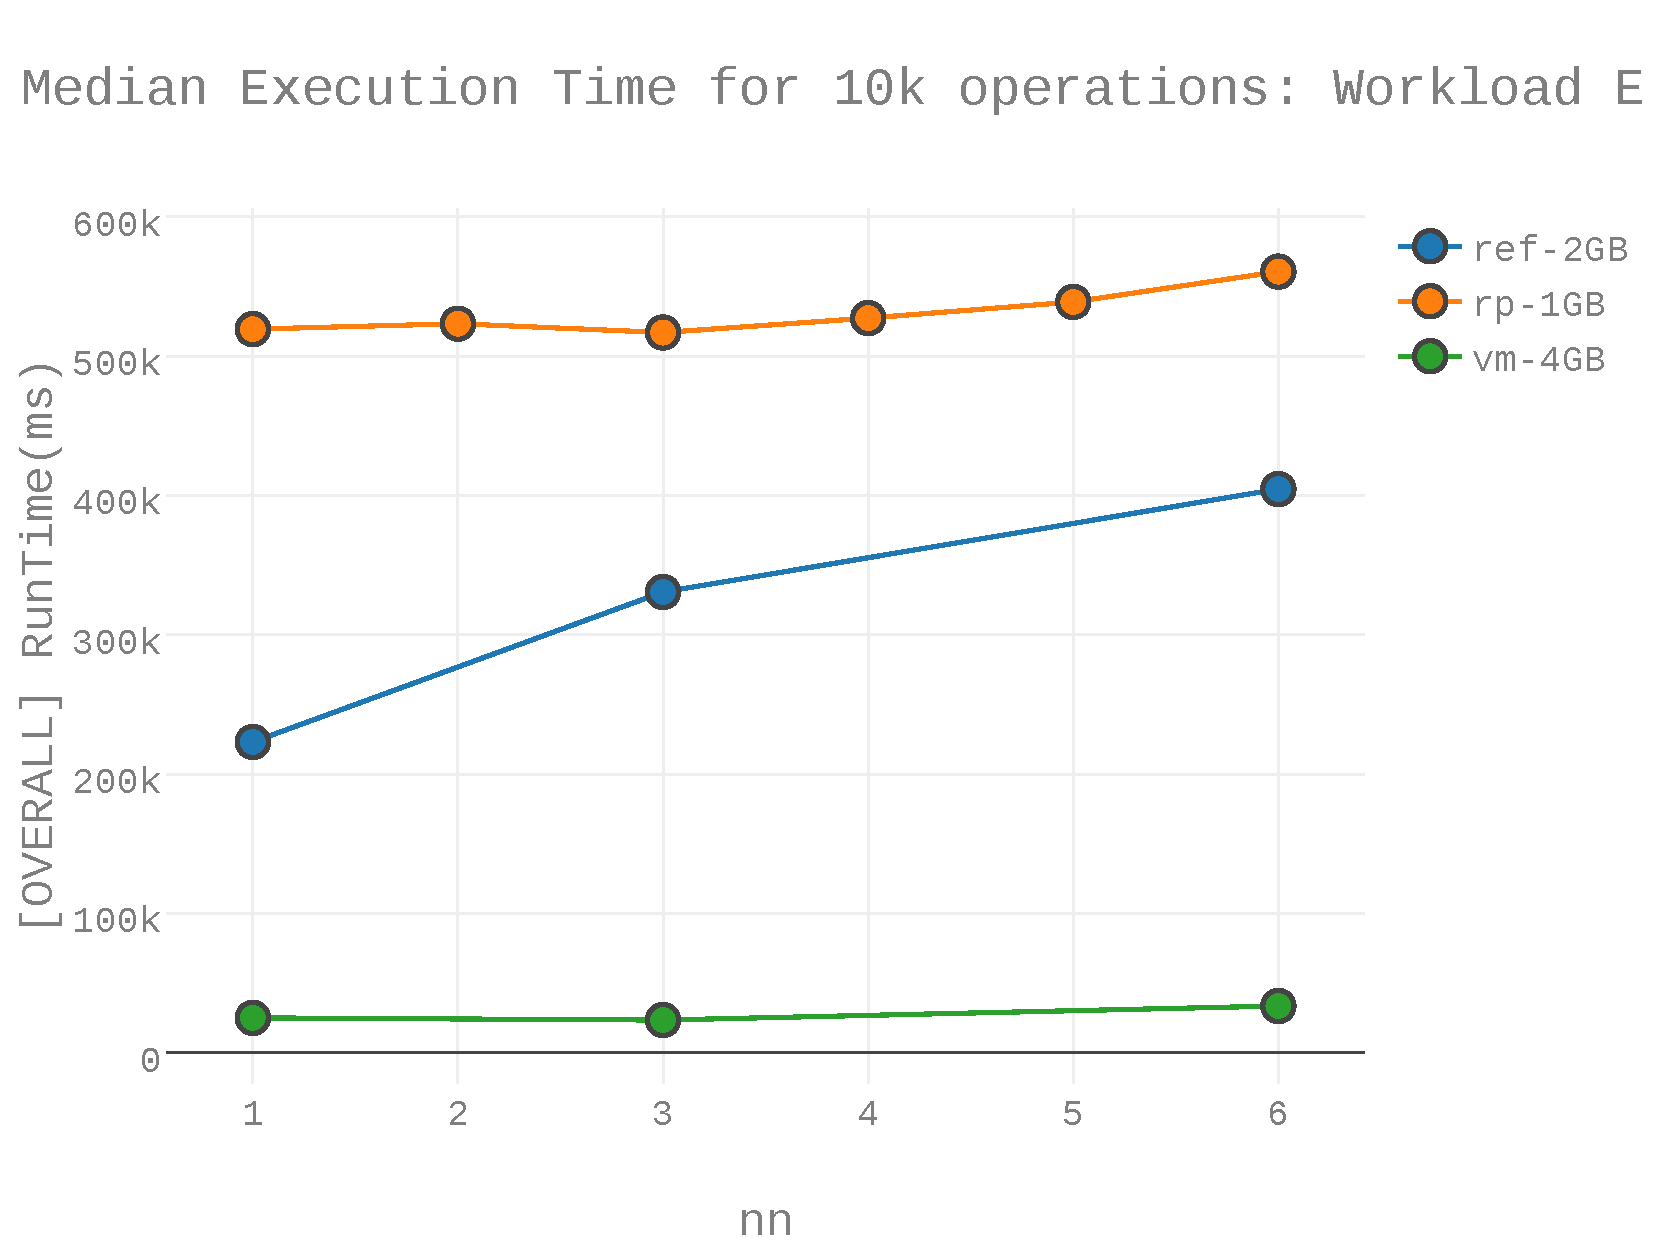
\includegraphics[width=3.5in]{Figures/figures-wle_fig6.pdf}

\caption{Comparison between the Raspberry Pi nodes (rp-1GB), the results reported in \cite{Abramova2014} (ref-2GB), and the virtual nodes with 4GB available \gls{ram} (vm-4GB).}

\label{fig:fig06}
\end{figure}

\begin{table}
\begin{tabular}{lrrr}
\toprule
 index &       1 &       3 &       6 \\
\midrule
 count &      21 &      21 &      21 \\
  mean & 5.2e+05 & 5.2e+05 & 5.6e+05 \\
   std & 2.1e+03 & 5.5e+03 &   3e+03 \\
   min & 5.2e+05 & 5.1e+05 & 5.6e+05 \\
   25\% & 5.2e+05 & 5.1e+05 & 5.6e+05 \\
   50\% & 5.2e+05 & 5.2e+05 & 5.6e+05 \\
   75\% & 5.2e+05 & 5.2e+05 & 5.6e+05 \\
   max & 5.2e+05 & 5.3e+05 & 5.7e+05 \\
 range & 8.3e+03 &   2e+04 &   1e+04 \\
\bottomrule
\end{tabular}
\caption{Summary for Raspberry Pi wired local area network}
\label{table:rp_wired_summary_statistics}
\end{table}

As can be seen from Figure \ref{fig:fig06}, the Raspberry Pi configuration takes considerably more execution time than the virtual machine analogy, which is probably due to the physical nature of the Ethernet connections (propagation delay) and the I/O limitations of the Raspberry Pi hardware.  However, its seemingly similar performance to the reference in \cite{Abramova2014} suggests the \gls{io} for the \gls{sd} Card follows a predictable pattern, and actually seems to outperform the node in \cite{Abramova2014} in the degenerate 1-node case.

For this paragraph, consider the results from \cite{Abramova2014} as the reference.  For a node network of 1, the experimental values fell between 515941.0 ms and 524199.0 ms, inclusive, and all values fell within 301019.0 ms of the reference value of 223180 ms.  For a node network of 3, the experimental values fell between 511997.0 ms and 532260.0 ms, inclusive, and all values fell within 201440.0 ms of the reference value of 330820 ms.  For a node network of 6, the experimental values fell between 555007.0 ms and 565388.0 ms, inclusive, and all values fell within 160728.0 ms of the reference value of 404660 ms.  

\subsection{Raspberry Pi versus the Reference Value}

For {} out of {} nodes, the reference value 

\subsubsection{Initial Observations}

%--fig1--%


\subsubsection{Ordinal Statistics}

\subsubsection{Speedup Analysis}



\subsection{Raspberry Pi versus the Virtual Machine}

\subsubsection{Initial Observations}

\subsubsection{Ordinal Statistics}

\subsubsection{Speedup Analysis}

\subsection{Wireless Links Only}

\subsubsection{Initial Observations}

\subsubsection{Ordinal Statistics}

\subsubsection{Scalability Analysis}

\subsection{Wireless Links versus Wired Links}

\subsubsection{Initial Observations}

\subsubsection{Ordinal Statistics}

\subsubsection{Speedup From Wired Links}

The median value of the corresponding wired experiment will serve as the reference in this paragraph. For a node network of 1, the experimental values fell between 625938.0 ms and 724603.0 ms, inclusive, and all values fell within 204854.0 ms of the reference value of 519749.0 ms.  For a node network of 3, the experimental values fell between 1198600.0 ms and 1458086.0 ms, inclusive, and all values fell within 941493.0 ms of the reference value of 516593.0 ms.  For a node network of 6, the experimental values fell between 260.0 ms and 2018342.0 ms, inclusive, and all values fell within 1459859.0 ms of the reference value of 558483.0 ms.  

\begin{figure}[h]
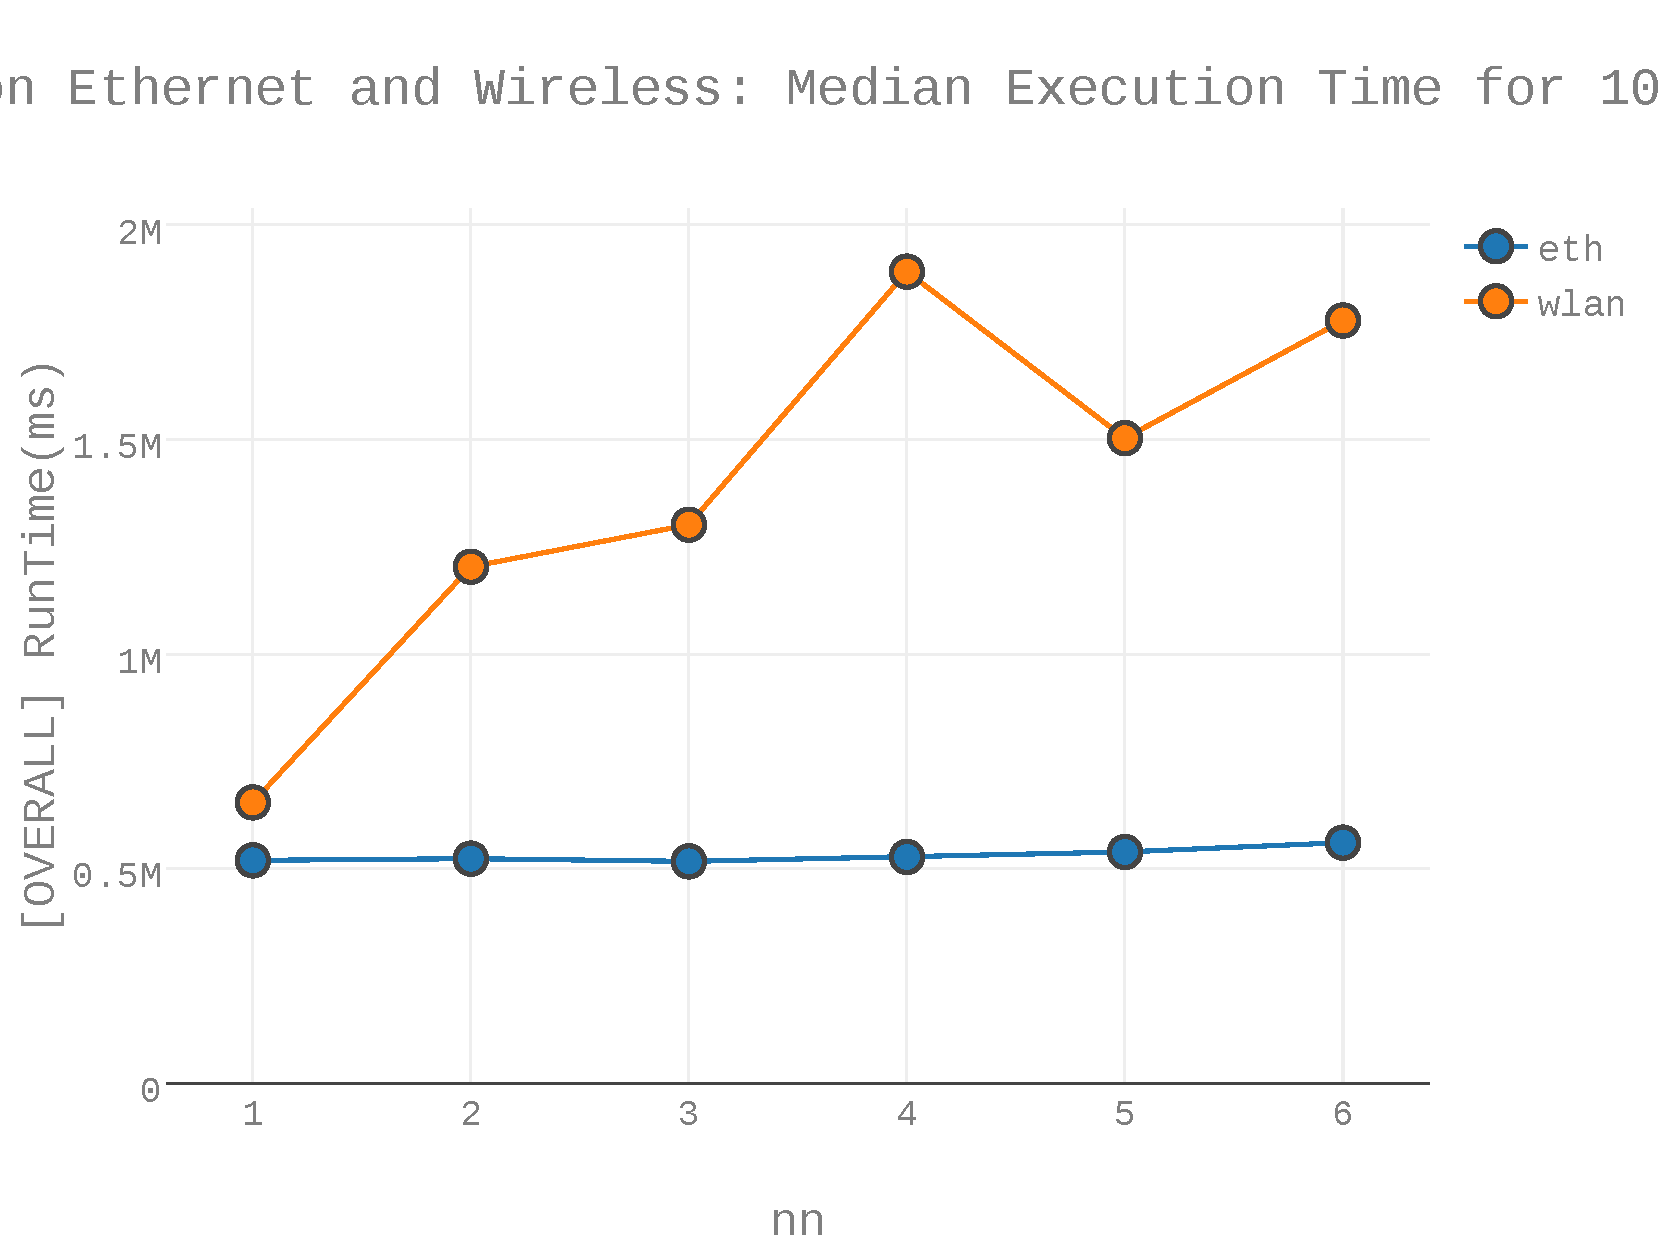
\includegraphics[width=3.5in]{Figures/figures-wle_fig7.pdf}

\caption{Comparison between the Ethernet links (eth) and wireless links (wlan) using the Raspberry Pi nodes.}

\label{fig:fig07}
\end{figure}

Figure \ref{fig:fig07} depicts the two experiments using Raspberry Pis: a wireless LAN (wlan) and an Ethernet LAN (eth).  In Figure \ref{fig:fig07}, as well as previous graphs, one can observe that the the Ethernet LAN effects about 50 seconds of execution time for 10,000 operations.  The initial median execution time for a node on a wireless LAN was found to be double the execution time.

For both configurations, performance takes a hit when transitioning from 1 to 2 nodes, but then increases from 2 nodes to 3 nodes.  From 3 nodes to 4 nodes, the wireless LAN configuration’s performance decreases dramatically, compared to slight increase in the wired Ethernet case.  

\begin{figure}[h]
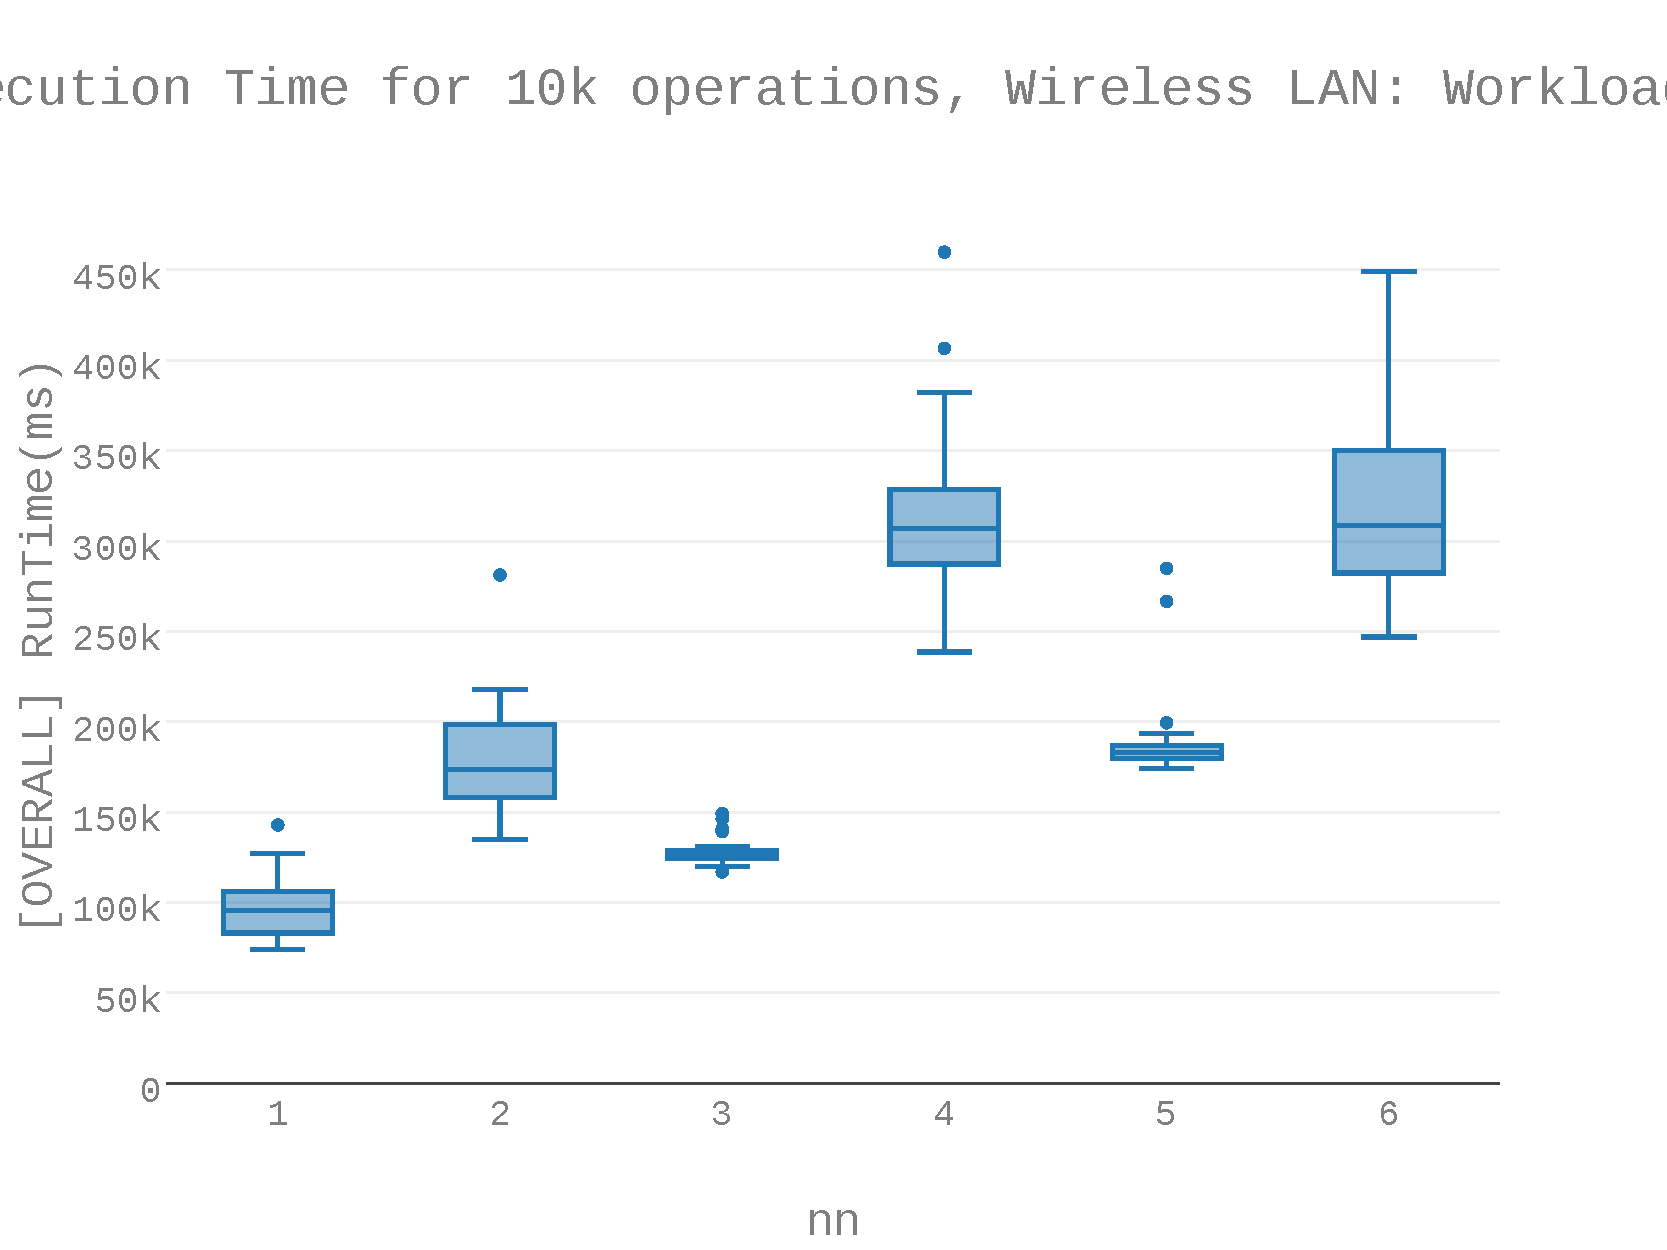
\includegraphics[width=3.5in]{Figures/figures-wle_fig8.pdf}

\caption{Distribution for all 30 trials of execution times where the Raspberry Pi nodes were connected via a wireless \gls{lan}.  Suspected outliers, values more than 3 times the interquartile range, are included as individual points above and below the 'maximum' and 'minimum' bars.}

\label{fig:fig08}
\end{figure}

A summary representation box plot of the results of wireless experimentation is above.  Here, the laptop was connected to the router via an Ethernet cable, and each node was connected to the router on a wireless local area network (LAN).  Suspected outliers, values more than 3 times the interquartile range (IQR) are included as points above and below.
There seems to be an overall increasing trend, while the data seems to oscillate, performing better for odd (1,3,5 node) configurations than for even (2,4,6 node) configurations.  However, there is no current theory behind this anomaly. 

\begin{figure}[h]
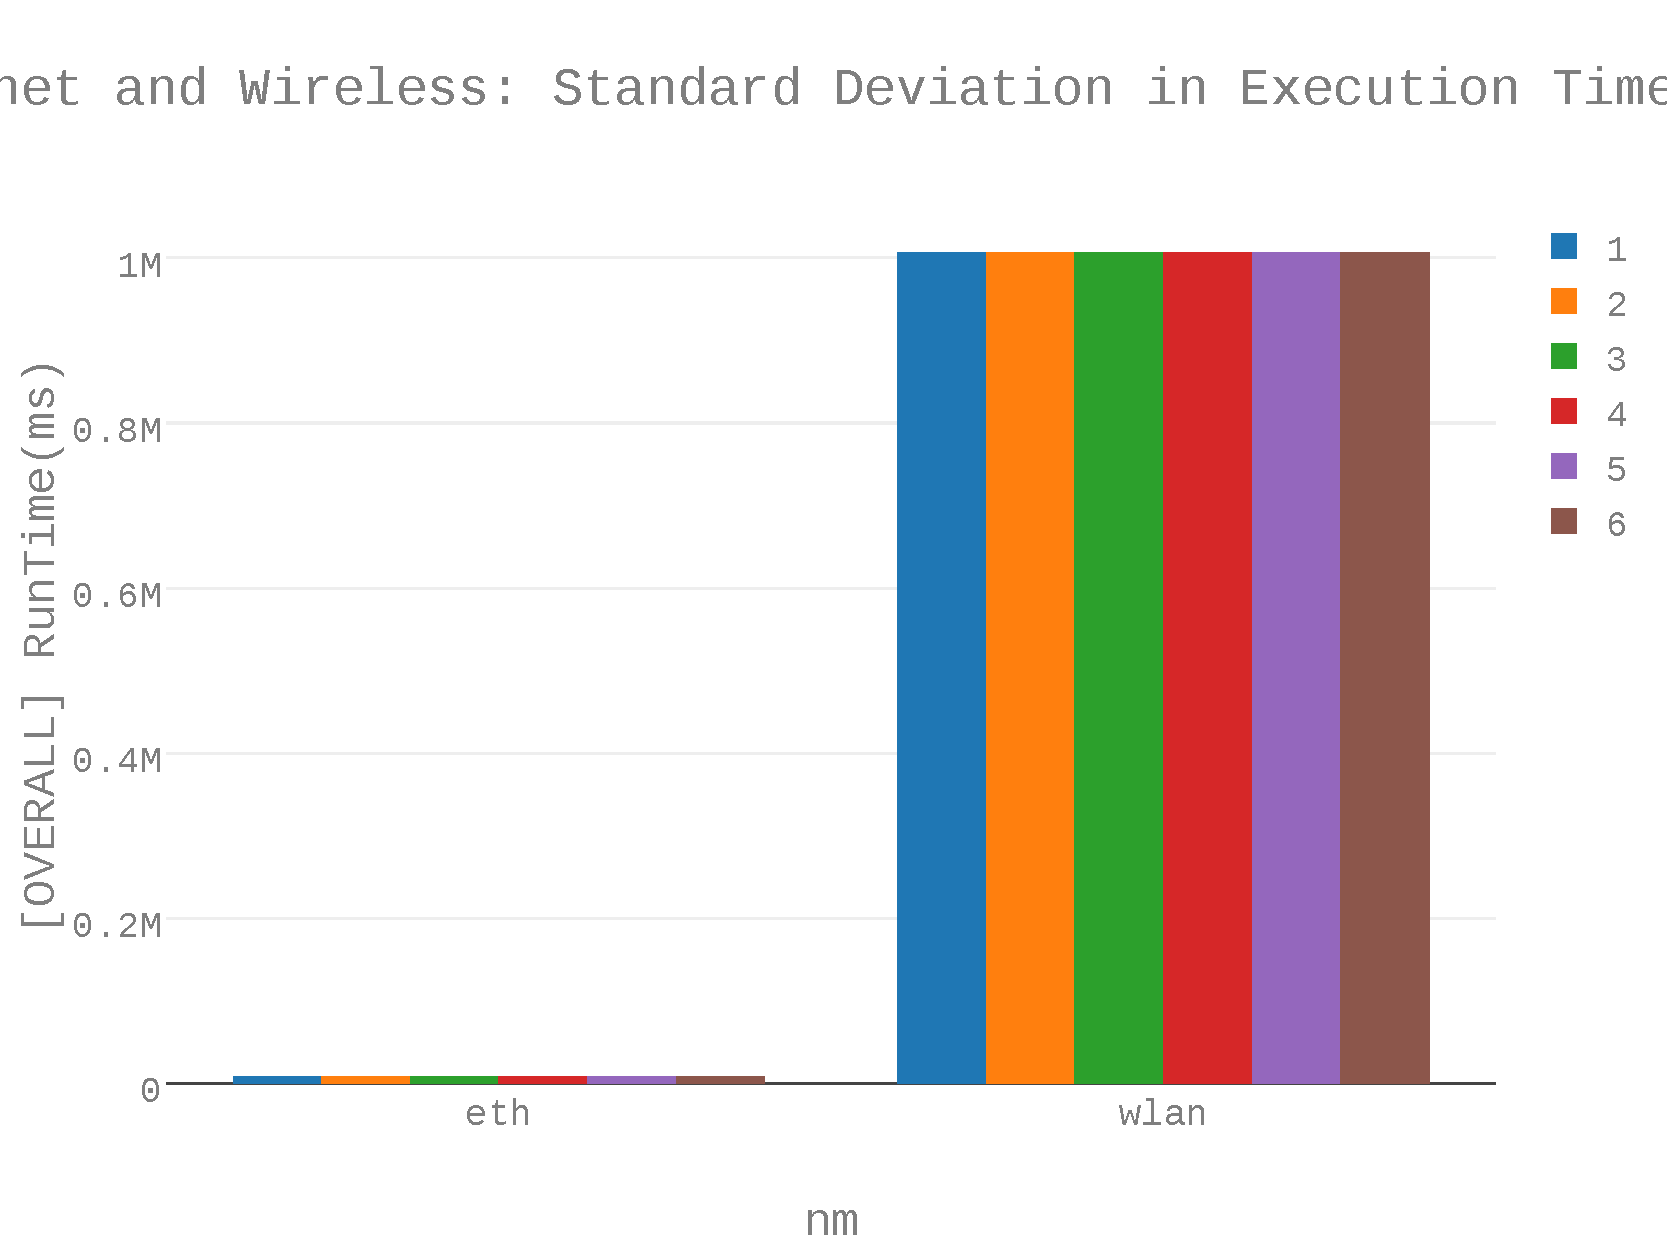
\includegraphics[width=3.5in]{Figures/figures-wle_fig9.pdf}

\caption{This compares the standard deviation in execution times for 10,000 operations of Workload C on the wired (eth) versus the wireless (wlan) configurations for 1 node, 2 nodes, 3 nodes, up through 6 nodes in milliseconds.}

\label{fig:fig09}
\end{figure}

To supplement the box plot, the standard deviation execution times for each set of trials, separated by number of nodes, is depicted in Figure \ref{fig:fig09}.  The difference seen here appears stark, and is overwhelming compared to the variance between 1, 2, 3, 4, 5 and 6 node networks given the same communication method. 

%1)      Reduced performance of Workload A is not statistically significant for the reduced memory sizes of IoT like devices
%2)      When varying platforms, performance for Workload A tracks the performance of the reference paper. For trials performe, reduced performance of Workload A is within 100ms of the reference paper (abramova) for wired implementations.
%3)      When varying communication method, reduced performance of Workload A is within 100ms of the wired platform test (order of magnitude, no greater than 100% increase in delay)
%4)      Reduced performance of Workload C is not statistically significant for the reduced memory sizes of IoT like devices
%5)      When varying platforms, reduced performance of Workload C is within 100ms of the reference paper (abramova) for wired implementations
%6)      When varying communication method, reduced performance of Workload C is within 100ms of the wired platform test
%7)      Reduced performance of Workload E is not statistically significant for the reduced memory sizes of IoT like devices
%8)      When varying platforms, reduced performance of Workload E is within 100ms of the reference paper (abramova) for wired implementations
%9)      When varying communication method, reduced performance of Workload E is within 100ms of the wired platform test



\chapter{Results and Evaluation}
\section{Results for Workload A}
\subsection{Comparing Existing Work: Virtual Machine vs the Reference Value}
\subsubsection{Initial Observations}
The result medians are displayed in Figure \ref{figures-wla_fig5}.  As expected, the virtual machine results imply much, much less execution time compared to the reference value, presumably accounting for diminished network latency. Such network latency seems to have an increasing effect on the reference as the cluster size goes up, but further analysis would be required to even make this claim. \begin{figure}[h]
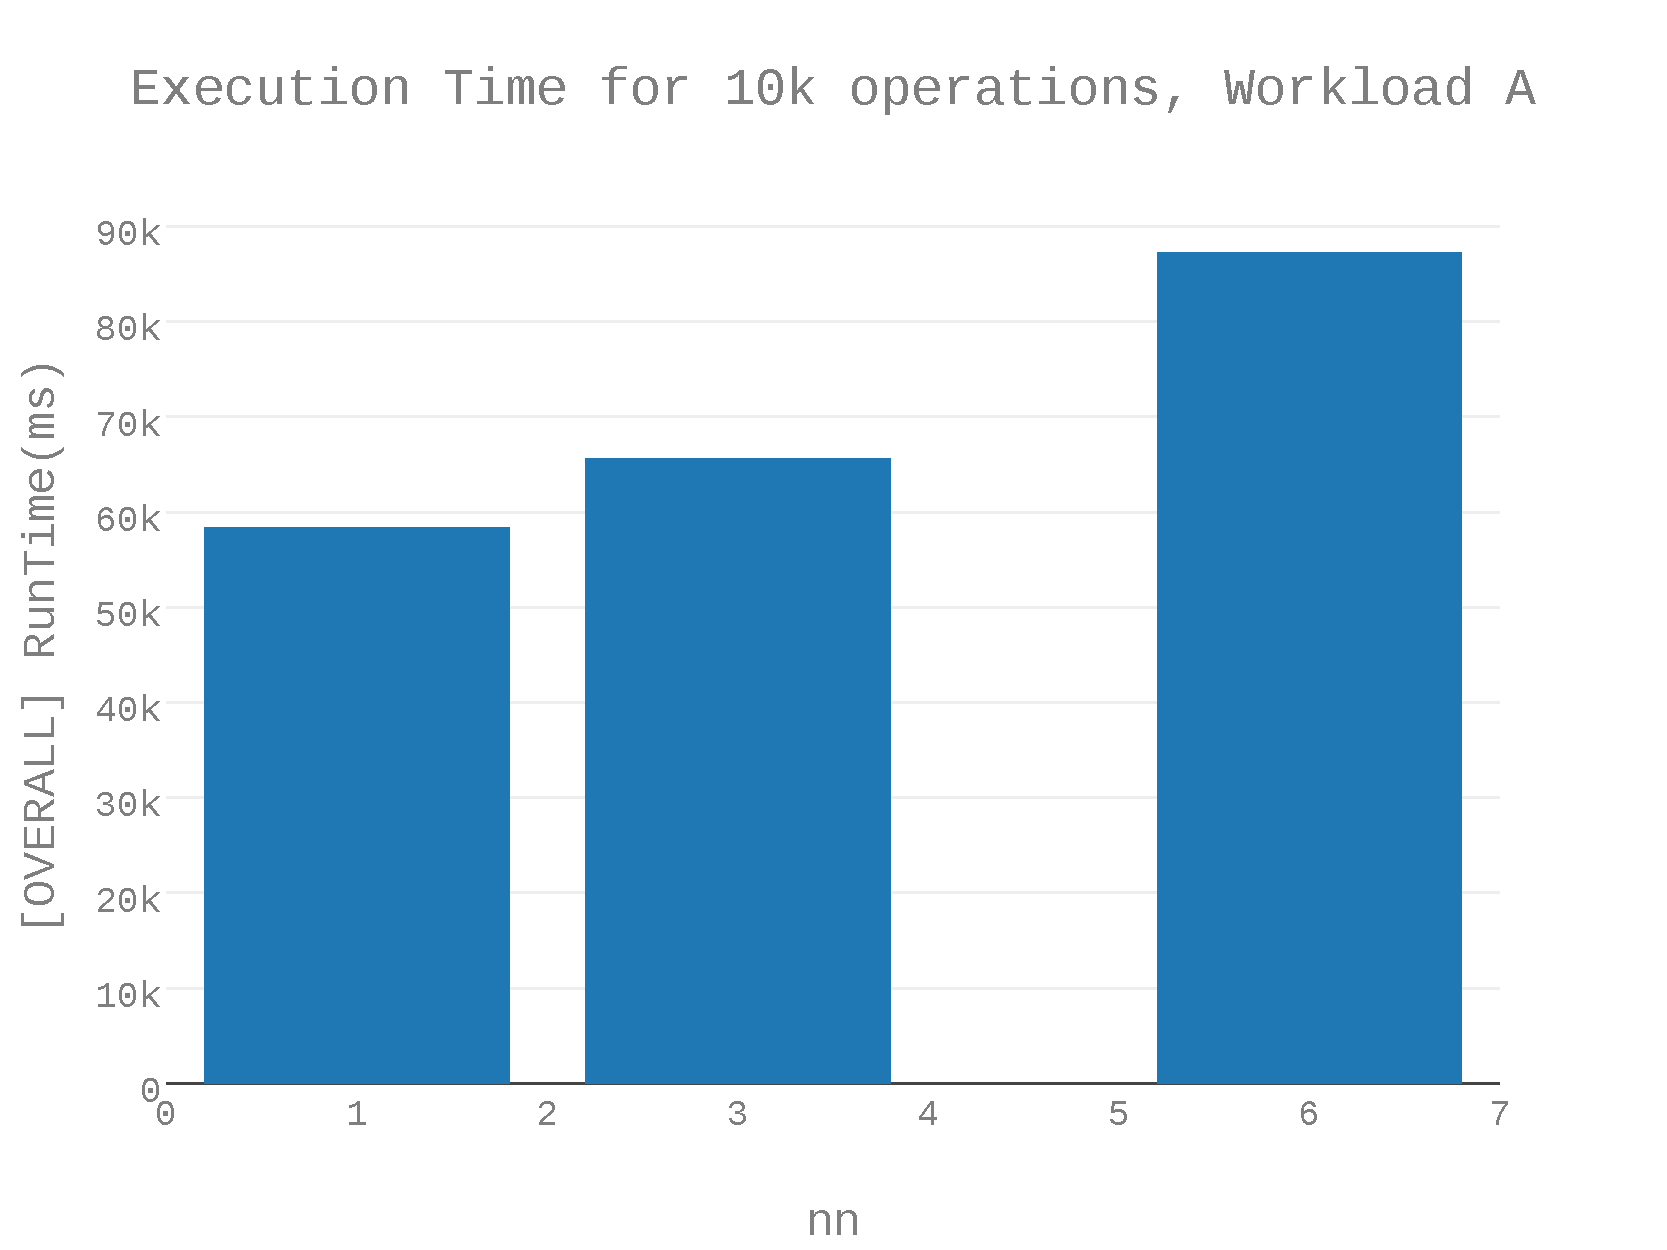
\includegraphics[width=5.5in]{Figures/figures-wla_fig1.pdf}
\caption{}
\label{figures-wla_fig1}
\end{figure}

\begin{figure}[h]
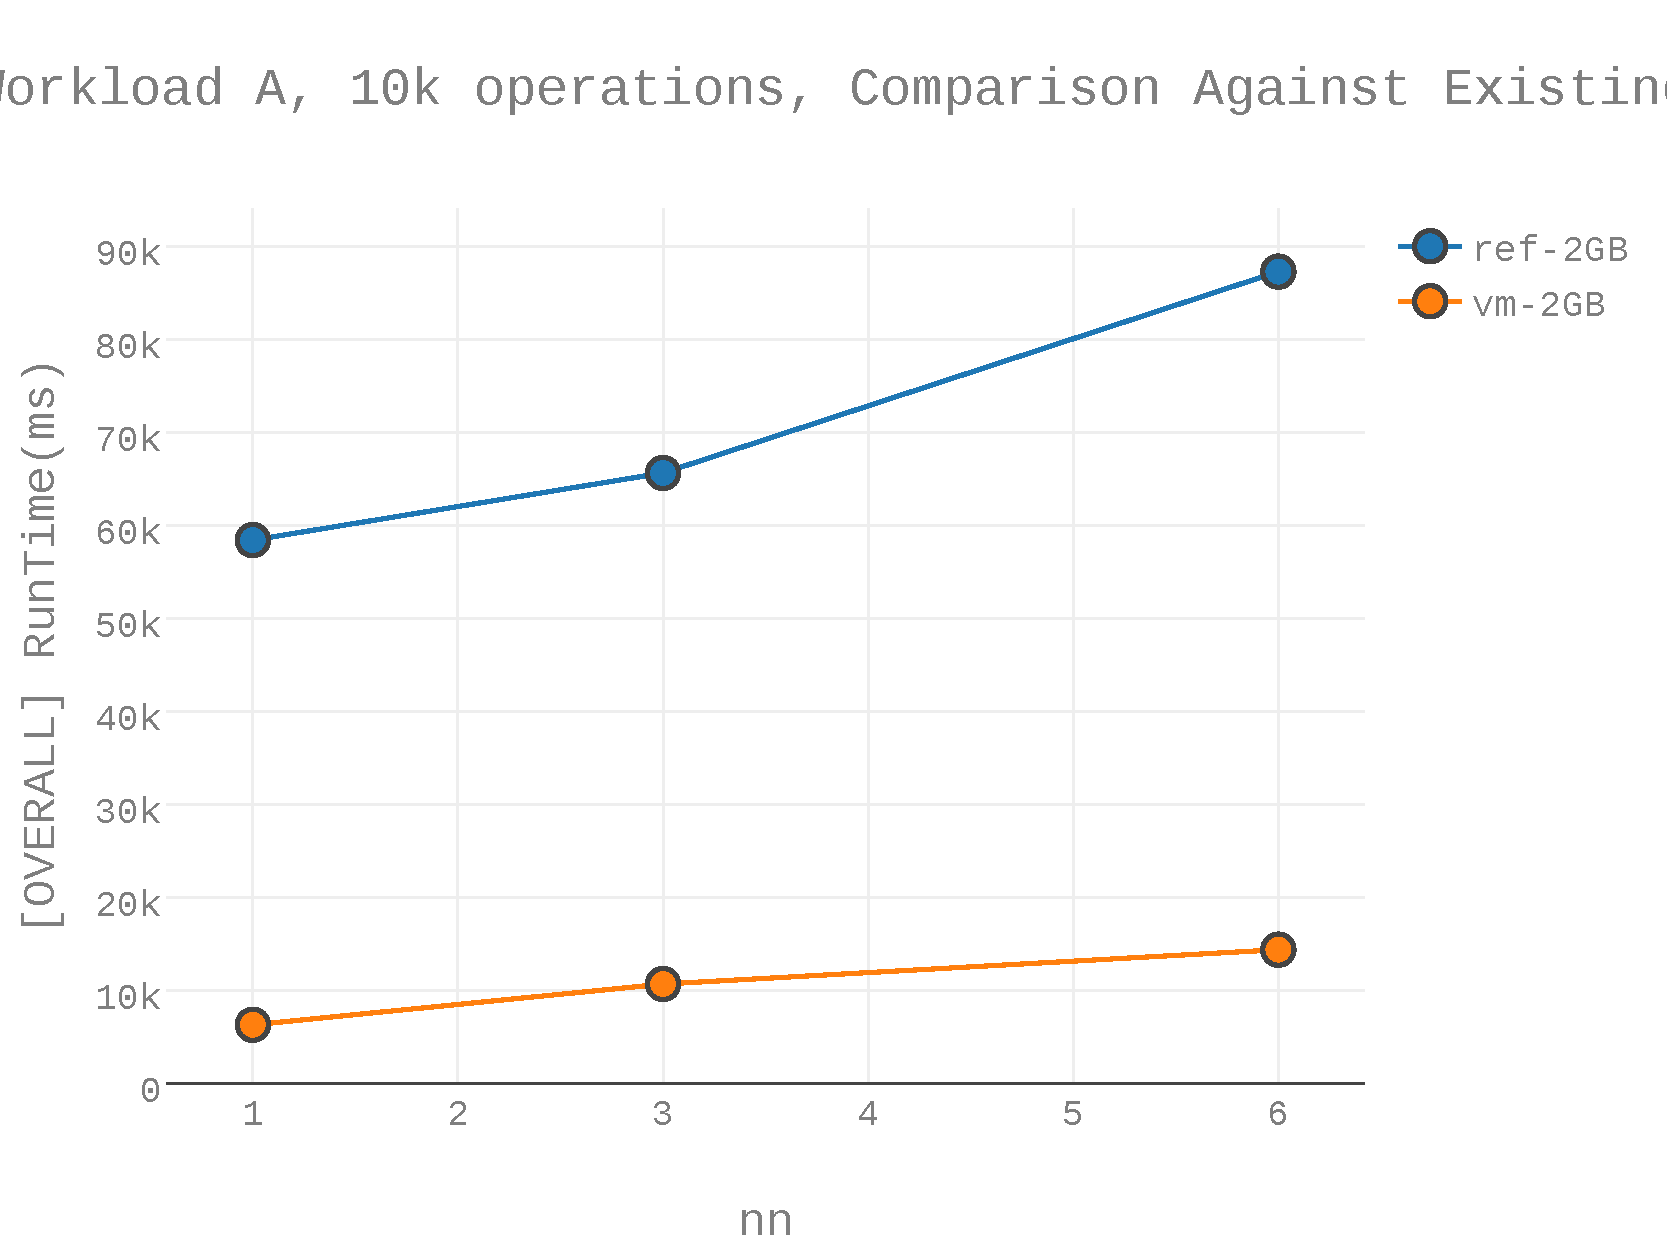
\includegraphics[width=5.5in]{Figures/figures-wla_fig5.pdf}
\caption{}
\label{figures-wla_fig5}
\end{figure}



\subsubsection{Ordinal Statistics}
This section will describe some of the summary statistics that describe the data.  

The summary statistics for Workload A performed on the virtual machines are in Tables \ref{table:summary_table_a_1GB_vm_nodal}, \ref{table:summary_table_a_2GB_vm_nodal}, and \ref{table:summary_table_a_4GB_vm_nodal}.
\begin{table}
\begin{tabular}{lrrrr}
\toprule
cluster\_size &     1.0 &     3.0 &     6.0 &  Overall \\
\midrule
25\%   & 6.2e+03 &   1e+04 & 1.4e+04 &  6.3e+03 \\
50\%   & 6.3e+03 &   1e+04 & 1.4e+04 &    1e+04 \\
75\%   & 6.3e+03 & 1.1e+04 & 1.4e+04 &  1.4e+04 \\
count &      21 &      21 &      21 &       63 \\
max   & 6.3e+03 & 1.1e+04 & 1.5e+04 &  1.5e+04 \\
mean  & 6.2e+03 & 1.1e+04 & 1.4e+04 &    1e+04 \\
min   & 6.1e+03 &   1e+04 & 1.4e+04 &  6.1e+03 \\
range & 2.8e+02 & 6.8e+02 & 6.8e+02 &  8.6e+03 \\
std   &      84 & 2.2e+02 & 1.7e+02 &  3.3e+03 \\
\bottomrule
\end{tabular}
\caption{Summary Statistics for Workload A performed on a 2GB virtual machine node over a(n)nodal network.  Except for count, all values are in milliseconds.}
\label{table:summary_table_a_2GB_vm_nodal}
\end{table}



\subsubsection{Analysis}
This section will take a more in-depth look at the data.
:::something went wrong generating the speedup analysis tables:::

\subsection{1GB RAM vs 2GB RAM vs 4GB RAM}
\subsubsection{Initial Observations}
This section discusses testing and performance for memory sizes: 1GB, 2GB, and 4GB.  The results are displayed in Figure \ref{figures-wla_fig4}. While it appears the varying the amount of memory has some effect on the results, theredoes not seem to be a predictable pattern across nodes. An ANOVA test will determine if there is an effect, and a linear regression will further testfor an effect. \begin{figure}[h]
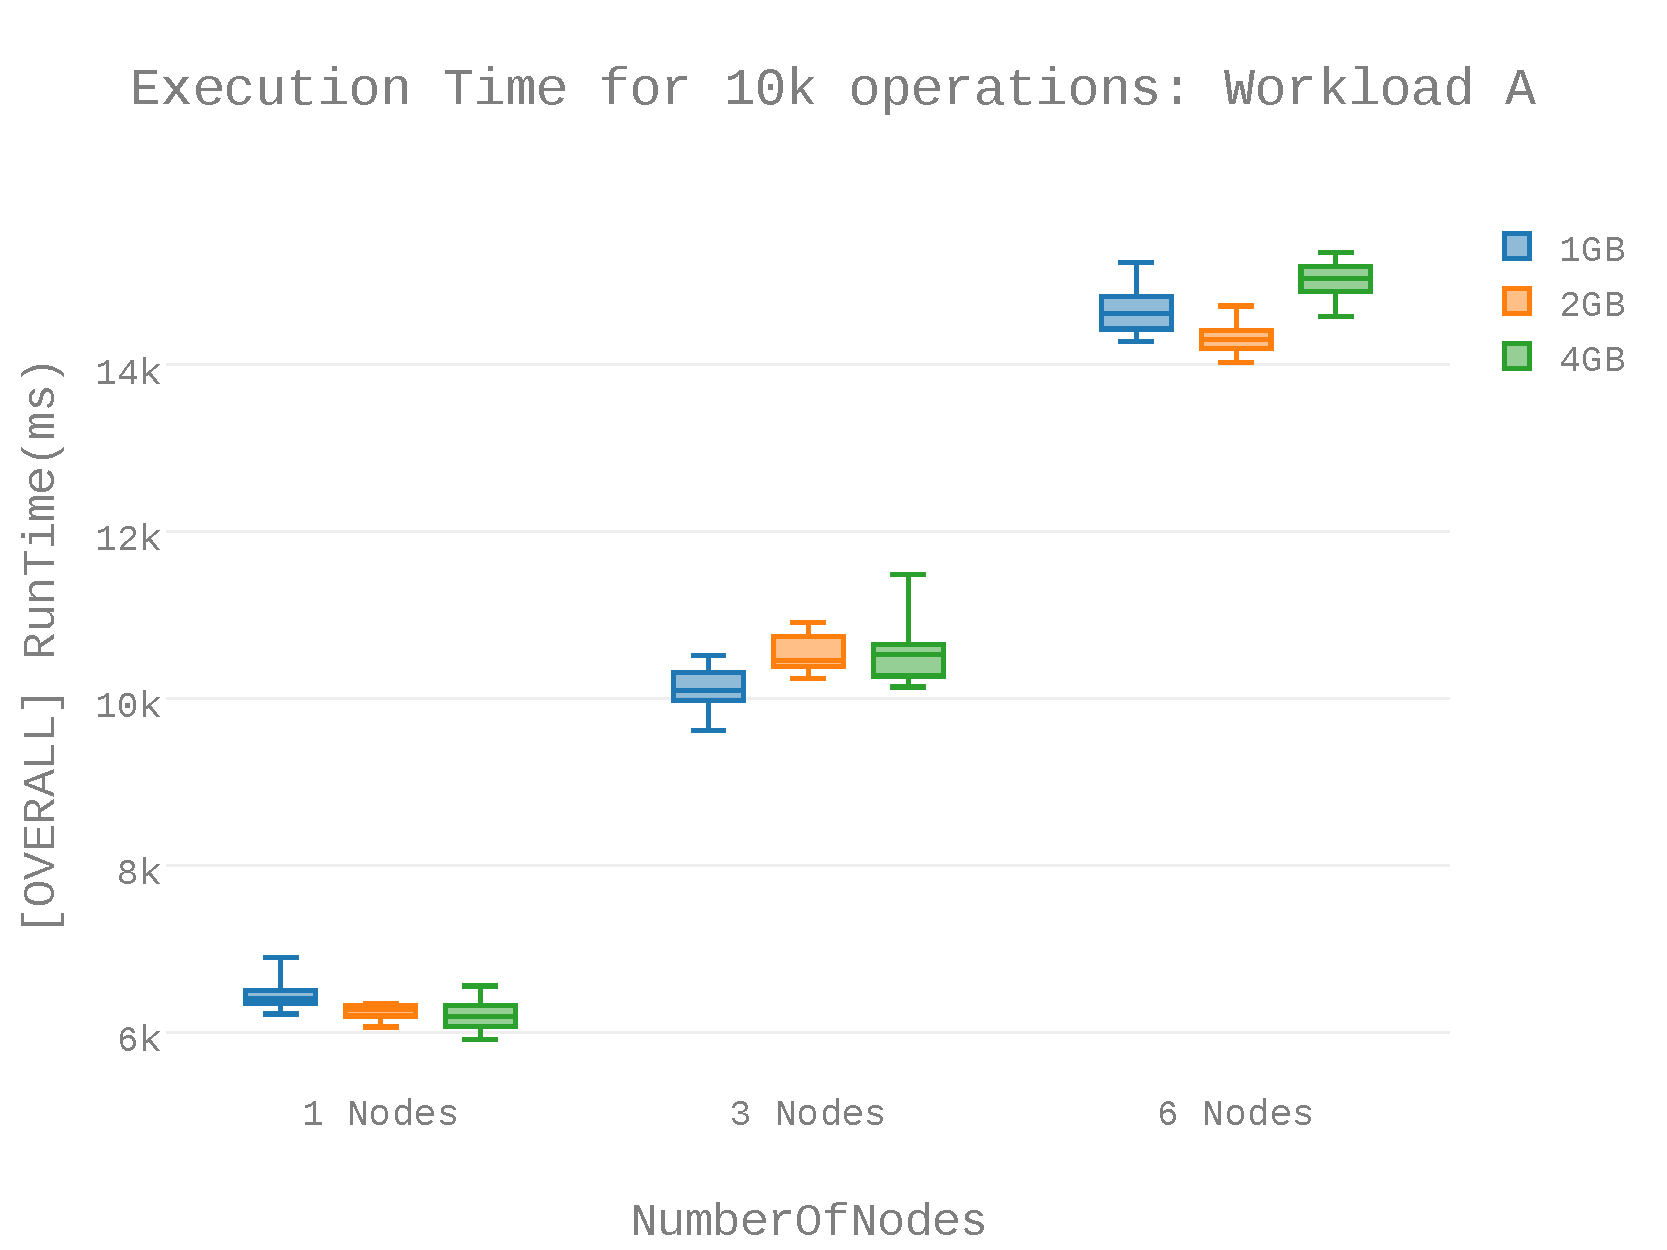
\includegraphics[width=5.5in]{Figures/figures-wla_fig4.pdf}
\caption{}
\label{figures-wla_fig4}
\end{figure}



\subsubsection{Ordinal Statistics}
This section will describe some of the summary statistics that describe the data.  

The summary statistics for Workload A performed on the virtual machines are in Tables \ref{table:summary_table_a_1GB_vm_nodal}, \ref{table:summary_table_a_2GB_vm_nodal}, and \ref{table:summary_table_a_4GB_vm_nodal}.
\begin{table}
\begin{tabular}{lrrrr}
\toprule
cluster\_size &     1.0 &     3.0 &     6.0 &  Overall \\
\midrule
25\%   & 6.4e+03 &   1e+04 & 1.4e+04 &  6.5e+03 \\
50\%   & 6.4e+03 &   1e+04 & 1.5e+04 &    1e+04 \\
75\%   & 6.5e+03 &   1e+04 & 1.5e+04 &  1.4e+04 \\
count &      21 &      21 &      21 &       63 \\
max   & 6.9e+03 & 1.1e+04 & 1.5e+04 &  1.5e+04 \\
mean  & 6.4e+03 &   1e+04 & 1.5e+04 &    1e+04 \\
min   & 6.2e+03 & 9.6e+03 & 1.4e+04 &  6.2e+03 \\
range & 6.7e+02 &   9e+02 & 9.5e+02 &    9e+03 \\
std   & 1.4e+02 & 2.3e+02 & 2.7e+02 &  3.4e+03 \\
\bottomrule
\end{tabular}
\caption{Summary Statistics for Workload A performed on a 1GB virtual machine node over a(n)nodal network.  Except for count, all values are in milliseconds.}
\label{table:summary_table_a_1GB_vm_nodal}
\end{table}

\begin{table}
\begin{tabular}{lrrrr}
\toprule
cluster\_size &     1.0 &     3.0 &     6.0 &  Overall \\
\midrule
25\%   & 6.1e+03 &   1e+04 & 1.5e+04 &  6.3e+03 \\
50\%   & 6.2e+03 & 1.1e+04 & 1.5e+04 &  1.1e+04 \\
75\%   & 6.3e+03 & 1.1e+04 & 1.5e+04 &  1.5e+04 \\
count &      21 &      21 &      21 &       63 \\
max   & 6.6e+03 & 1.1e+04 & 1.5e+04 &  1.5e+04 \\
mean  & 6.2e+03 & 1.1e+04 & 1.5e+04 &  1.1e+04 \\
min   & 5.9e+03 &   1e+04 & 1.5e+04 &  5.9e+03 \\
range & 6.4e+02 & 1.3e+03 & 7.7e+02 &  9.4e+03 \\
std   & 1.7e+02 & 3.4e+02 & 2.2e+02 &  3.6e+03 \\
\bottomrule
\end{tabular}
\caption{Summary Statistics for Workload A performed on a 4GB virtual machine node over a(n)nodal network.  Except for count, all values are in milliseconds.}
\label{table:summary_table_a_4GB_vm_nodal}
\end{table}




\subsubsection{Analysis}
This section will take a more in-depth look at the data.


\begin{table}[H]
\centering
\begin{tabular}{rrrrrr}
\toprule
 cluster\_size &   slope &  intercept &  r\_value &  p\_value &  std\_err \\
\midrule
            1 &     -69 &    6.5e+03 &    -0.51 &  2.1e-05 &       15 \\
            3 & 1.2e+02 &      1e+04 &     0.46 &  0.00016 &       30 \\
            6 & 1.5e+02 &    1.4e+04 &     0.51 &  1.7e-05 &       32 \\
\bottomrule
\end{tabular}
\caption{Linear Regression over amount of RAM}
\label{table:ram_v_ram_a}
\end{table}



\subsection{Implementation on Raspberry Pi}
\subsubsection{Initial Observations}
The results are displayed in Figure \ref{figures-wla_fig10}.  \begin{figure}[h]
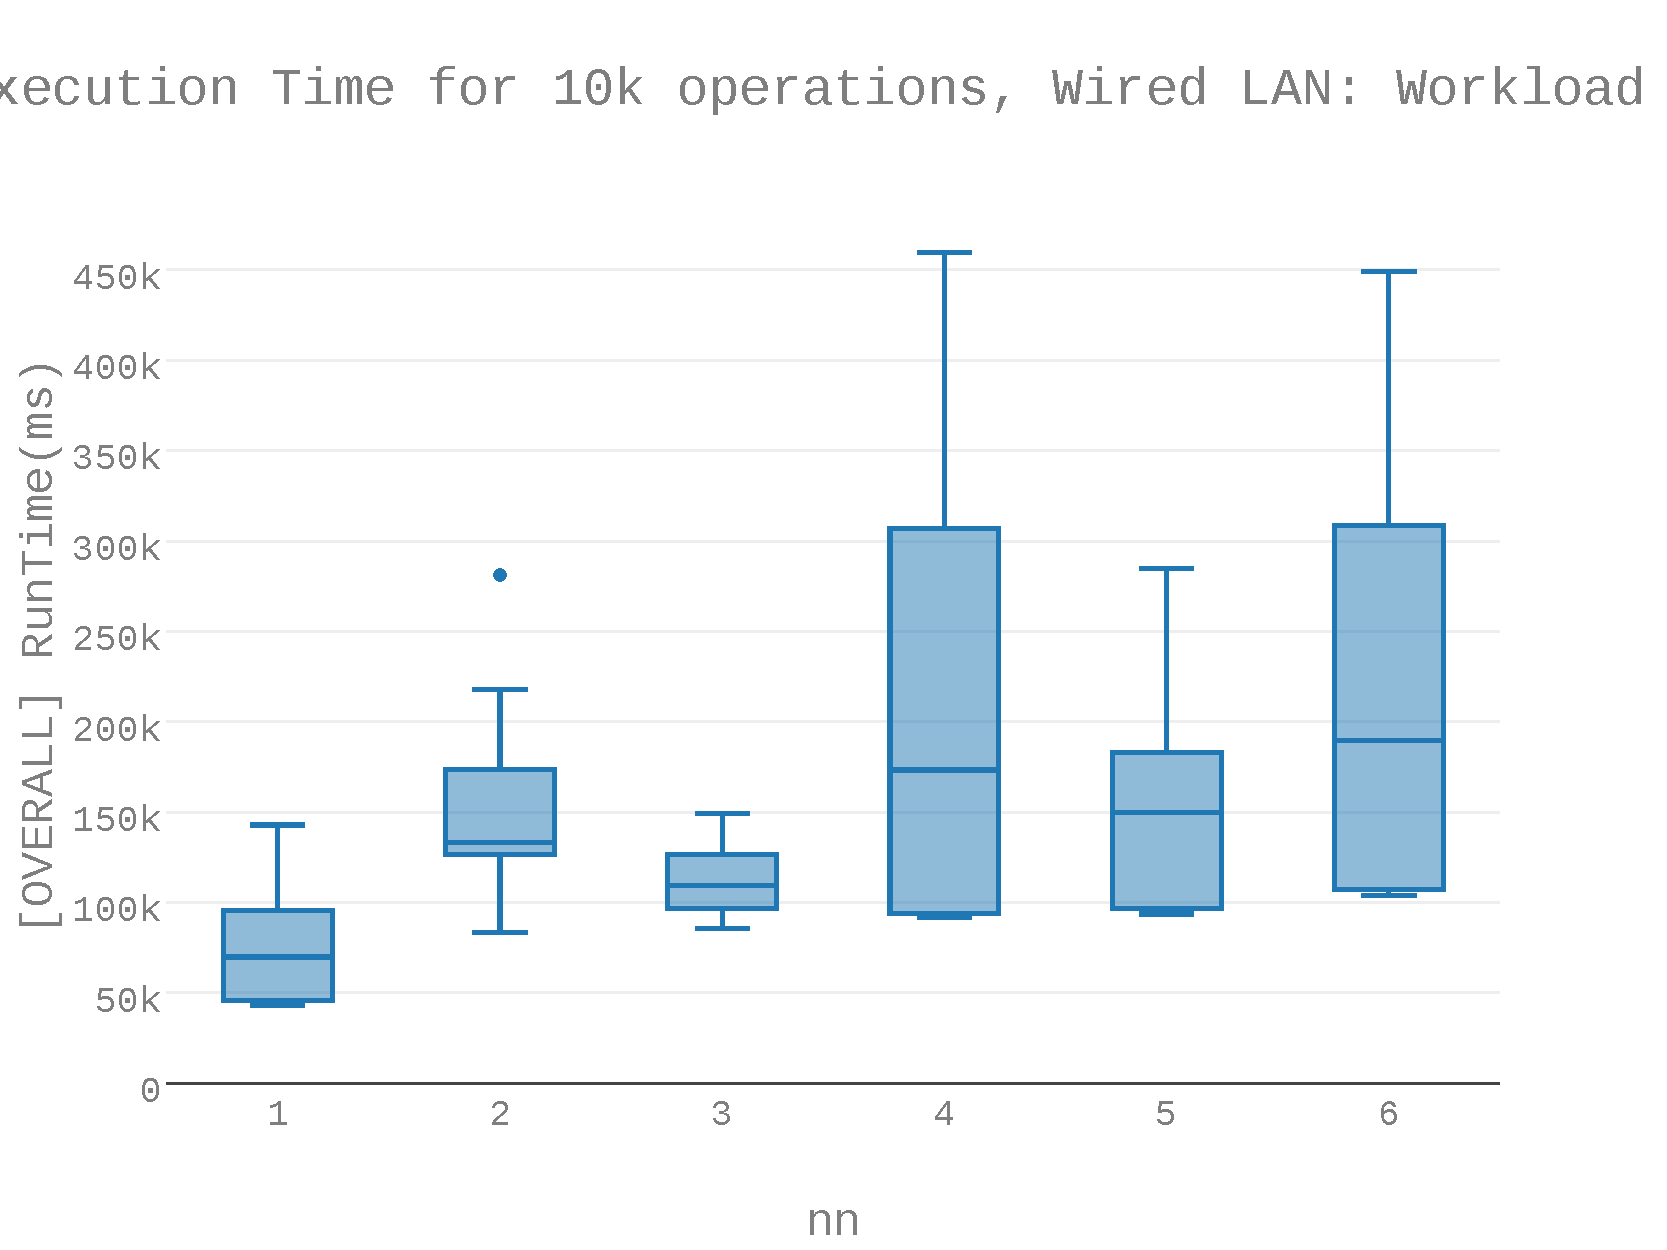
\includegraphics[width=5.5in]{Figures/figures-wla_fig10.pdf}
\caption{}
\label{figures-wla_fig10}
\end{figure}



\subsubsection{Ordinal Statistics}
This section will describe some of the summary statistics that describe the data.  

The summary statistics for Workload A performed on the limited hardware, Raspberry Pi, on the Ethernet local area network are in Table \ref{table:summary_table_a_1GB_rp_eth}.
\begin{table}
\begin{tabular}{lrrrrrrr}
\toprule
cluster\_size &     1.0 &     2.0 &     3.0 &     4.0 &     5.0 &     6.0 &  Overall \\
\midrule
25\%   & 4.5e+04 & 1.3e+05 & 9.6e+04 & 9.4e+04 & 9.6e+04 & 1.1e+05 &  9.4e+04 \\
50\%   & 4.6e+04 & 1.3e+05 & 9.7e+04 & 9.4e+04 & 9.6e+04 & 1.1e+05 &  9.7e+04 \\
75\%   & 4.6e+04 & 1.3e+05 & 9.8e+04 & 9.5e+04 & 9.8e+04 & 1.1e+05 &  1.1e+05 \\
count &      21 &      21 &      21 &      21 &      21 &      21 &  1.3e+02 \\
max   & 4.8e+04 & 1.3e+05 &   1e+05 & 9.6e+04 & 9.9e+04 & 1.1e+05 &  1.3e+05 \\
mean  & 4.6e+04 & 1.3e+05 & 9.7e+04 & 9.4e+04 & 9.6e+04 & 1.1e+05 &  9.5e+04 \\
min   & 4.3e+04 & 1.2e+05 & 9.4e+04 & 9.3e+04 & 9.4e+04 &   1e+05 &  4.3e+04 \\
range & 4.9e+03 & 1.5e+04 & 6.8e+03 & 3.6e+03 & 4.9e+03 & 7.3e+03 &  8.8e+04 \\
std   & 1.1e+03 & 3.5e+03 & 1.6e+03 & 9.2e+02 & 1.5e+03 & 1.8e+03 &  2.5e+04 \\
\bottomrule
\end{tabular}
\caption{Summary Statistics for Workload A performed on a 1GB limited hardware, Raspberry Pi node over a(n)Ethernet network.  Except for count, all values are in milliseconds.}
\label{table:summary_table_a_1GB_rp_eth}
\end{table}



\subsubsection{Analysis}
This section will take a more in-depth look at the data.


\begin{table}[H]
\centering
\begin{tabular}{rrrrr}
\toprule
 slope &  intercept &  r\_value &  p\_value &  std\_err \\
\midrule
 6e+03 &    7.3e+04 &     0.42 &  1.1e-06 &  1.2e+03 \\
\bottomrule
\end{tabular}
\caption{Linear Regression over Cluster Size, Workload a}
\label{table:rp_only_a}
\end{table}



\subsection{Raspberry Pi vs Reference Value}
\subsubsection{Initial Observations}
The results are displayed in Figure \ref{figures-wla_fig6}.  The performance of the limited hardware, the Raspberry Pi, seems comparable with the results from the more appropriate in the other paper.  In addition, there is no reason to suspect a significant differential in the overall pattern with respect to scalability: performance over cluster size. \begin{figure}[h]
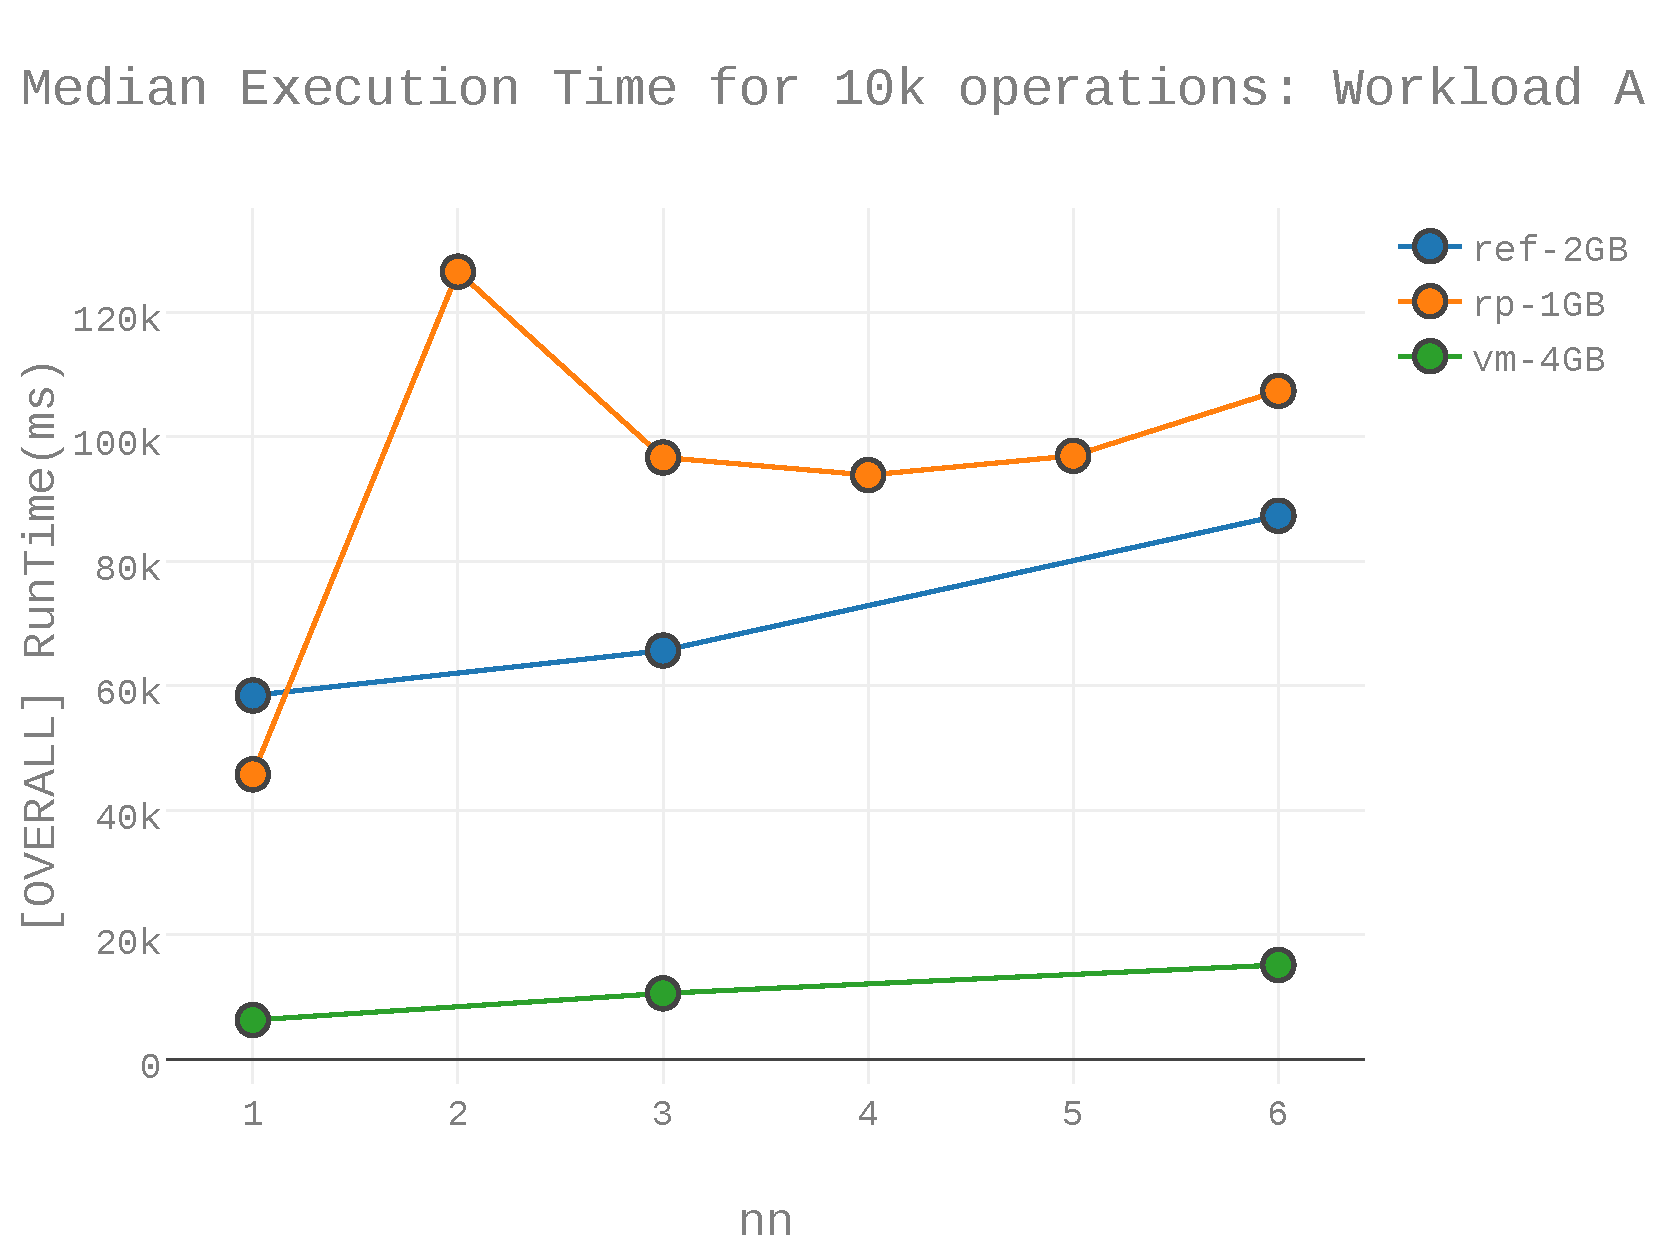
\includegraphics[width=5.5in]{Figures/figures-wla_fig6.pdf}
\caption{}
\label{figures-wla_fig6}
\end{figure}



\subsubsection{Ordinal Statistics}
This section will describe some of the summary statistics that describe the data.  

The summary statistics for Workload A performed on the limited hardware, Raspberry Pi, on the Ethernet local area network are in Table \ref{table:summary_table_a_1GB_rp_eth}.



\subsubsection{Analysis}
This section will take a more in-depth look at the data.
:::something went wrong generating the speedup analysis tables:::

\subsection{Raspberry Pi vs Virtual Machine}
\subsubsection{Initial Observations}
The results are displayed in Figure \ref{figures-wla_fig6}.  As expected, there is a significant differential between the limited hardware, the Raspberry Pi configuration and the virtual machine.  However, it is not clear if this is linear across cluster size. 

\subsubsection{Ordinal Statistics}
This section will describe some of the summary statistics that describe the data.  

The summary statistics for Workload A performed on the virtual machines are in Tables \ref{table:summary_table_a_1GB_vm_nodal}, \ref{table:summary_table_a_2GB_vm_nodal}, and \ref{table:summary_table_a_4GB_vm_nodal}.
The summary statistics for Workload A performed on the limited hardware, Raspberry Pi, on the Ethernet local area network are in Table \ref{table:summary_table_a_1GB_rp_eth}.



\subsubsection{Analysis}
This section will take a more in-depth look at the data.




\begin{table}[H]
\centering
\begin{tabular}{lrrrrr}
\toprule
cluster\_size &   slope &  intercept &  r\_value &  p\_value &  std\_err \\
\midrule
           1 & 3.9e+04 &    6.4e+03 &        1 &  1.3e-57 &  2.5e+02 \\
           2 &     nan &        nan &        0 &        1 &      inf \\
           3 & 8.7e+04 &      1e+04 &        1 &  8.6e-65 &  3.6e+02 \\
           4 &     nan &        nan &        0 &        1 &      inf \\
           5 &     nan &        nan &        0 &        1 &      inf \\
           6 & 9.2e+04 &    1.5e+04 &        1 &  2.3e-64 &  3.9e+02 \\
     OVERALL & 8.4e+04 &      1e+04 &     0.89 &  4.5e-66 &  3.1e+03 \\
\bottomrule
\end{tabular}
\caption{Linear Regression over the effect of limited hardware, Workload A}
\label{table:rp_v_vm_a}
\end{table}





\begin{table}[H]
\centering
\begin{tabular}{llllllll}
\toprule
{} &    0 &    1 &     2 &    3 &    4 &    5 &        6 \\
\midrule
cluster\_size         &    1 &    2 &     3 &    4 &    5 &    6 &  OVERALL \\
ratio\_max\_to\_min     & 0.16 &  NaN &  0.11 &  NaN &  NaN & 0.15 &     0.35 \\
ratio\_min\_to\_max     & 0.13 &  NaN & 0.096 &  NaN &  NaN & 0.13 &    0.047 \\
ratio\_of\_the\_means   & 0.14 &  NaN &   0.1 &  NaN &  NaN & 0.14 &     0.11 \\
ratio\_of\_the\_medians & 0.14 &  NaN &   0.1 &  NaN &  NaN & 0.14 &      0.1 \\
ratio\_of\_the\_stddevs & 0.13 &  NaN &  0.14 &  NaN &  NaN & 0.15 &     0.14 \\
\bottomrule
\end{tabular}
\caption{Speedup over the effect of limited hardware, Workload A}
\label{table:rp_v_vm_a_speedup}
\end{table}





\subsection{Wireless Links Only}
\subsubsection{Initial Observations}
The results are displayed in Figure \ref{figures-wla_fig8}.  Although there is a general trend of increased execution time over cluster size, the oscillation that occurs between odd and even node cluster sizes is hard to miss. This may be result of the collision avoidance strategy, but further experiments would be needed to determine a more specific explanation. \begin{figure}[h]
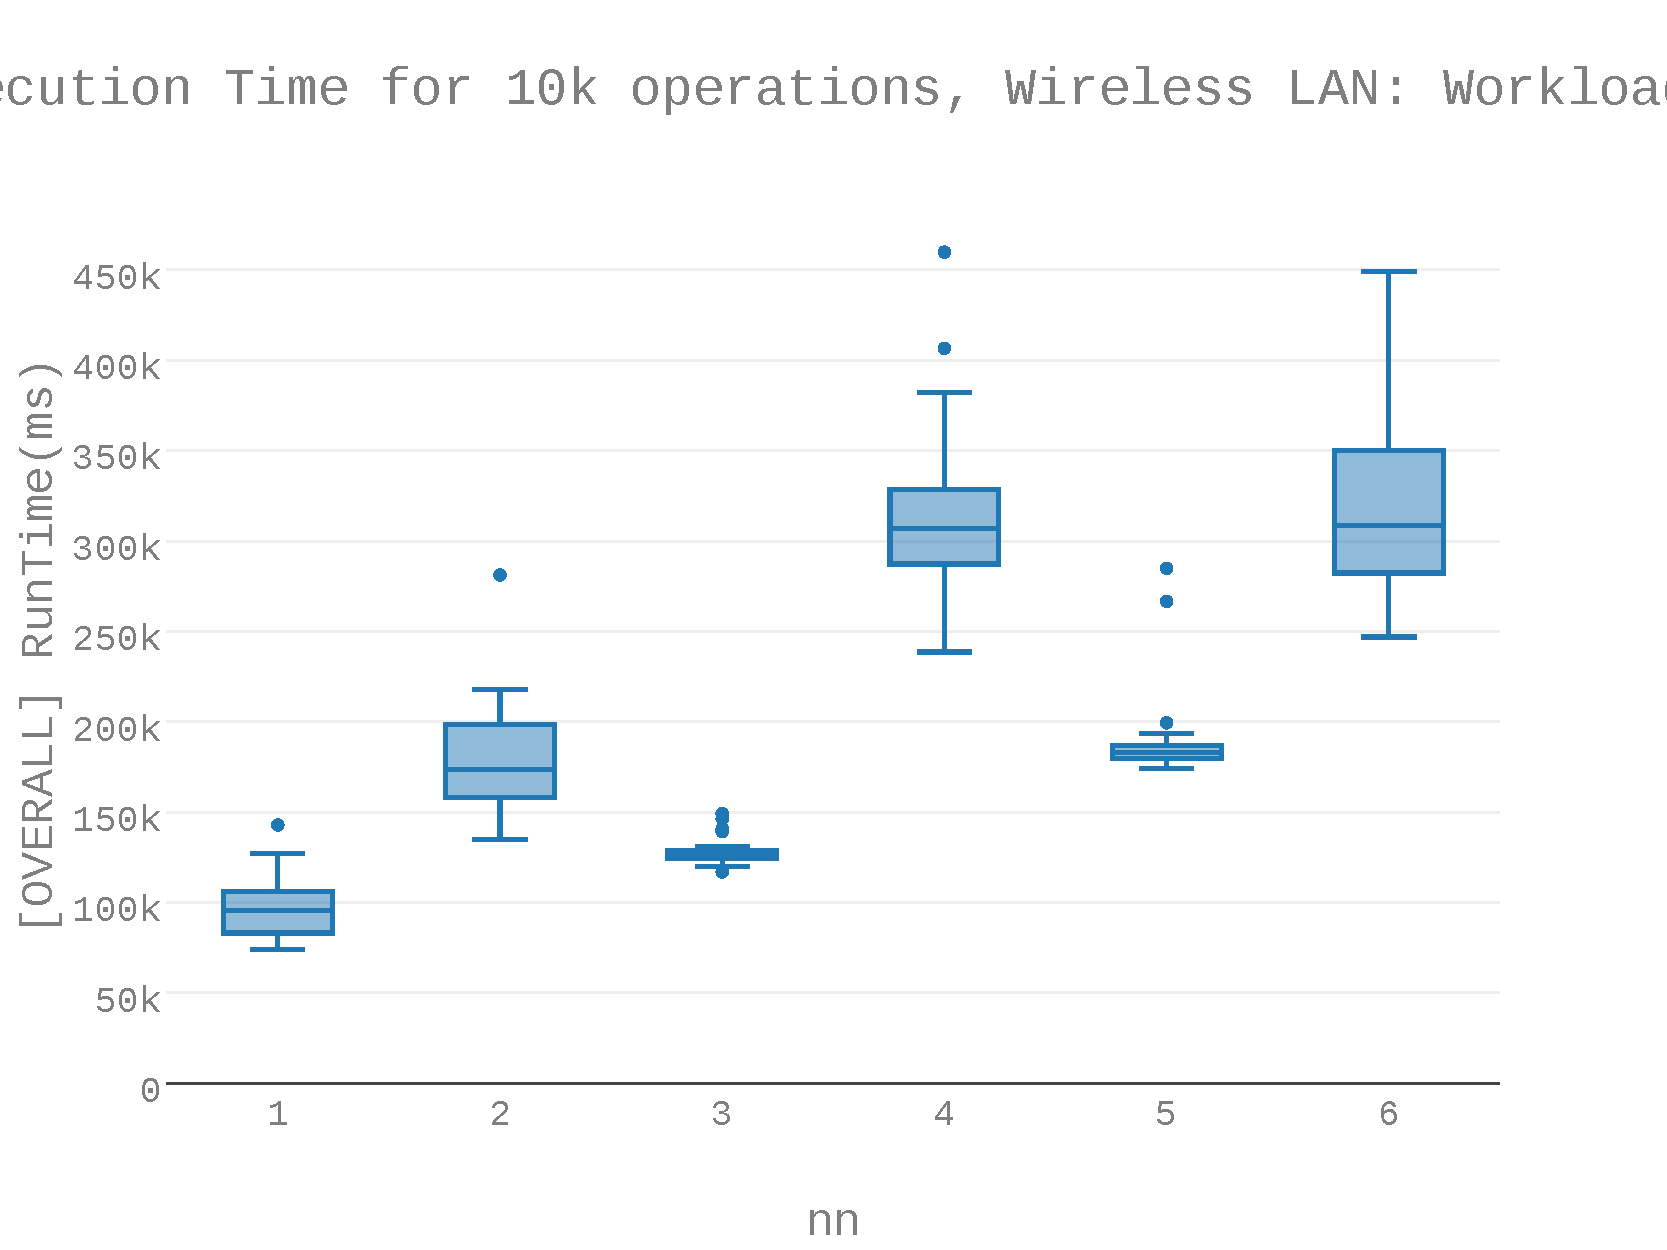
\includegraphics[width=5.5in]{Figures/figures-wla_fig8.pdf}
\caption{}
\label{figures-wla_fig8}
\end{figure}



\subsubsection{Ordinal Statistics}
This section will describe some of the summary statistics that describe the data.  

The summary statistics for Workload A performed on the limited hardware, Raspberry Pi, on the Ethernet local area network are in Table \ref{table:summary_table_a_1GB_rp_wlan}.
\begin{table}
\begin{tabular}{lrrrrrrr}
\toprule
cluster\_size &     1.0 &     2.0 &     3.0 &     4.0 &     5.0 &     6.0 &  Overall \\
\midrule
25\%   & 8.2e+04 & 1.7e+05 & 1.3e+05 &   3e+05 & 1.8e+05 & 2.7e+05 &  1.3e+05 \\
50\%   &   9e+04 & 1.8e+05 & 1.3e+05 & 3.2e+05 & 1.8e+05 &   3e+05 &  1.8e+05 \\
75\%   &   1e+05 &   2e+05 & 1.3e+05 & 3.3e+05 & 1.8e+05 & 3.1e+05 &  2.8e+05 \\
count &      21 &      21 &      21 &      21 &      21 &      21 &  1.3e+02 \\
max   & 1.2e+05 & 2.8e+05 & 1.5e+05 & 4.6e+05 & 2.8e+05 & 3.6e+05 &  4.6e+05 \\
mean  & 9.1e+04 & 1.9e+05 & 1.3e+05 & 3.2e+05 & 1.9e+05 &   3e+05 &    2e+05 \\
min   & 7.4e+04 & 1.5e+05 & 1.2e+05 & 2.6e+05 & 1.7e+05 & 2.5e+05 &  7.4e+04 \\
range & 4.6e+04 & 1.3e+05 & 2.6e+04 & 1.9e+05 & 1.1e+05 & 1.1e+05 &  3.9e+05 \\
std   & 1.3e+04 & 2.9e+04 & 7.4e+03 & 4.5e+04 & 2.9e+04 & 3.2e+04 &  8.7e+04 \\
\bottomrule
\end{tabular}
\caption{Summary Statistics for Workload A performed on a 1GB limited hardware, Raspberry Pi node over a(n)802.11a/b/g/n network.  Except for count, all values are in milliseconds.}
\label{table:summary_table_a_1GB_rp_wlan}
\end{table}



\subsubsection{Analysis}
This section will take a more in-depth look at the data.


\begin{table}[H]
\centering
\begin{tabular}{rrrrr}
\toprule
  slope &  intercept &  r\_value &  p\_value &  std\_err \\
\midrule
3.5e+04 &      8e+04 &     0.69 &  7.5e-19 &  3.3e+03 \\
\bottomrule
\end{tabular}
\caption{Linear Regression over Cluster Size, Workload a}
\label{table:wlan_only_a}
\end{table}



\subsection{Wireless Links vs Wired Links}
\subsubsection{Initial Observations}
The results are displayed in Figures \ref{figures-wla_fig7} and \ref{figures-wla_fig9}.  For 1, 2, and 3-node clusters, despite the expected  disparity in execution time, the wired and wireless trends seem to follow each other.  However, from 3 nodes up through 6 nodes, the execution times starts to diverge, suggesting that the wireless has a increasing effect as the number of nodes increases. \begin{figure}[h]
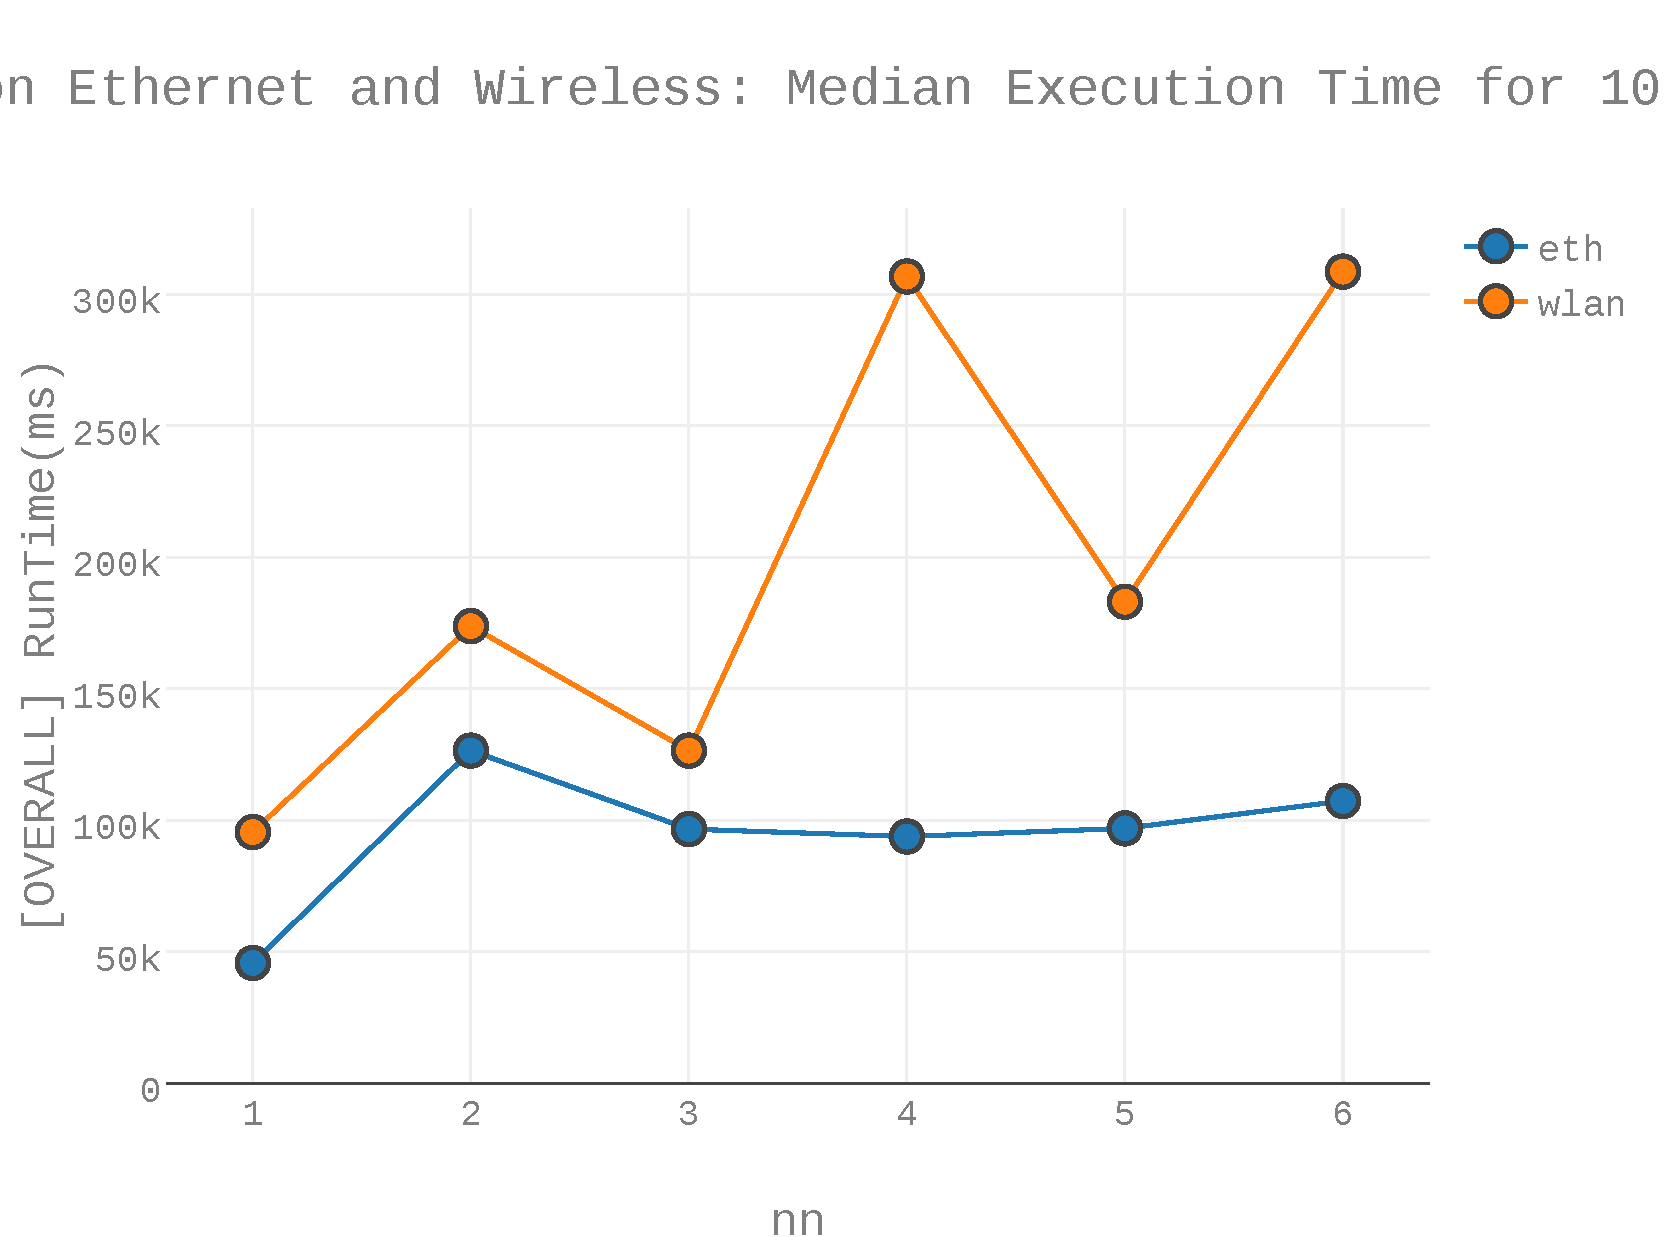
\includegraphics[width=5.5in]{Figures/figures-wla_fig7.pdf}
\caption{}
\label{figures-wla_fig7}
\end{figure}

\begin{figure}[h]
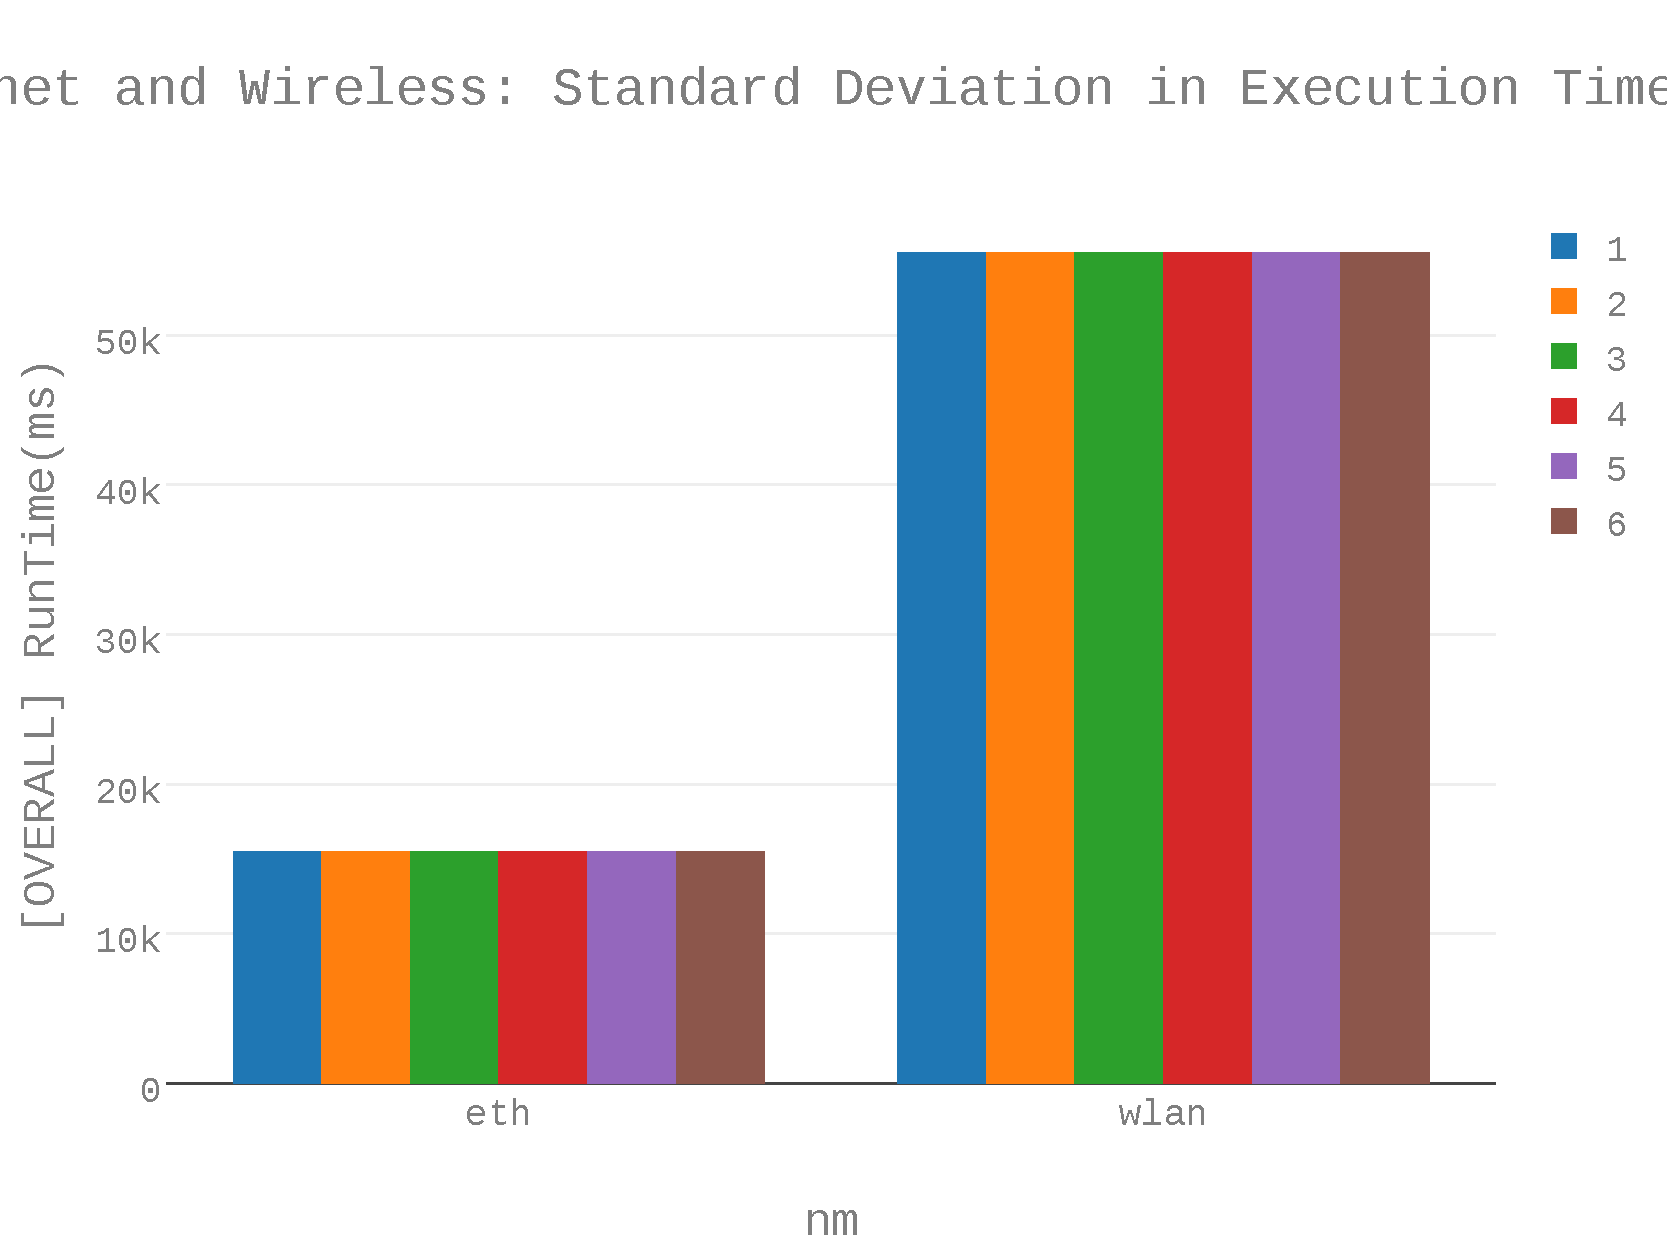
\includegraphics[width=5.5in]{Figures/figures-wla_fig9.pdf}
\caption{}
\label{figures-wla_fig9}
\end{figure}



\subsubsection{Ordinal Statistics}
This section will describe some of the summary statistics that describe the data.  

The summary statistics for Workload A performed on the limited hardware, Raspberry Pi, on the Ethernet local area network are in Table \ref{table:summary_table_a_1GB_rp_eth}.
The summary statistics for Workload A performed on the limited hardware, Raspberry Pi, on the Ethernet local area network are in Table \ref{table:summary_table_a_1GB_rp_wlan}.



\subsubsection{Analysis}
This section will take a more in-depth look at the data.




\begin{table}[H]
\centering
\begin{tabular}{lrrrrr}
\toprule
cluster\_size &   slope &  intercept &  r\_value &  p\_value &  std\_err \\
\midrule
           1 & 4.6e+04 &    4.6e+04 &     0.93 &  3.9e-19 &  2.8e+03 \\
           2 & 6.1e+04 &    1.3e+05 &     0.84 &  3.7e-12 &  6.3e+03 \\
           3 & 3.3e+04 &    9.7e+04 &     0.95 &  2.9e-22 &  1.7e+03 \\
           4 & 2.3e+05 &    9.4e+04 &     0.96 &  9.4e-25 &  9.8e+03 \\
           5 & 9.4e+04 &    9.6e+04 &     0.92 &  4.6e-18 &  6.3e+03 \\
           6 & 1.9e+05 &    1.1e+05 &     0.97 &  1.4e-27 &  6.9e+03 \\
     OVERALL & 1.1e+05 &    9.5e+04 &     0.65 &  3.4e-31 &  8.1e+03 \\
\bottomrule
\end{tabular}
\caption{Linear Regression over the effect of 802.11 links, Workload A}
\label{table:wlan_v_eth_a}
\end{table}





\begin{table}[H]
\centering
\begin{tabular}{llllllll}
\toprule
{} &     0 &    1 &    2 &    3 &     4 &     5 &        6 \\
\midrule
cluster\_size         &     1 &    2 &    3 &    4 &     5 &     6 &  OVERALL \\
ratio\_max\_to\_min     &  0.65 & 0.87 & 0.82 & 0.36 &  0.57 &  0.45 &      1.8 \\
ratio\_min\_to\_max     &  0.36 & 0.42 & 0.63 &  0.2 &  0.33 &  0.29 &    0.094 \\
ratio\_of\_the\_means   &   0.5 & 0.67 & 0.75 & 0.29 &  0.51 &  0.36 &     0.47 \\
ratio\_of\_the\_medians &  0.51 & 0.72 & 0.76 &  0.3 &  0.53 &  0.35 &     0.53 \\
ratio\_of\_the\_stddevs & 0.087 & 0.12 & 0.22 & 0.02 & 0.052 & 0.057 &     0.28 \\
\bottomrule
\end{tabular}
\caption{Speedup over the effect of 802.11 links, Workload A}
\label{table:wlan_v_eth_a_speedup}
\end{table}





\section{Results for Workload C}
\subsection{Comparing Existing Work: Virtual Machine vs the Reference Value}
\subsubsection{Initial Observations}
The result medians are displayed in Figure \ref{figures-wlc_fig5}.  As expected, the virtual machine results imply much, much less execution time compared to the reference value, presumably accounting for diminished network latency. Such network latency seems to have an increasing effect on the reference as the cluster size goes up, but further analysis would be required to even make this claim. \begin{figure}[h]
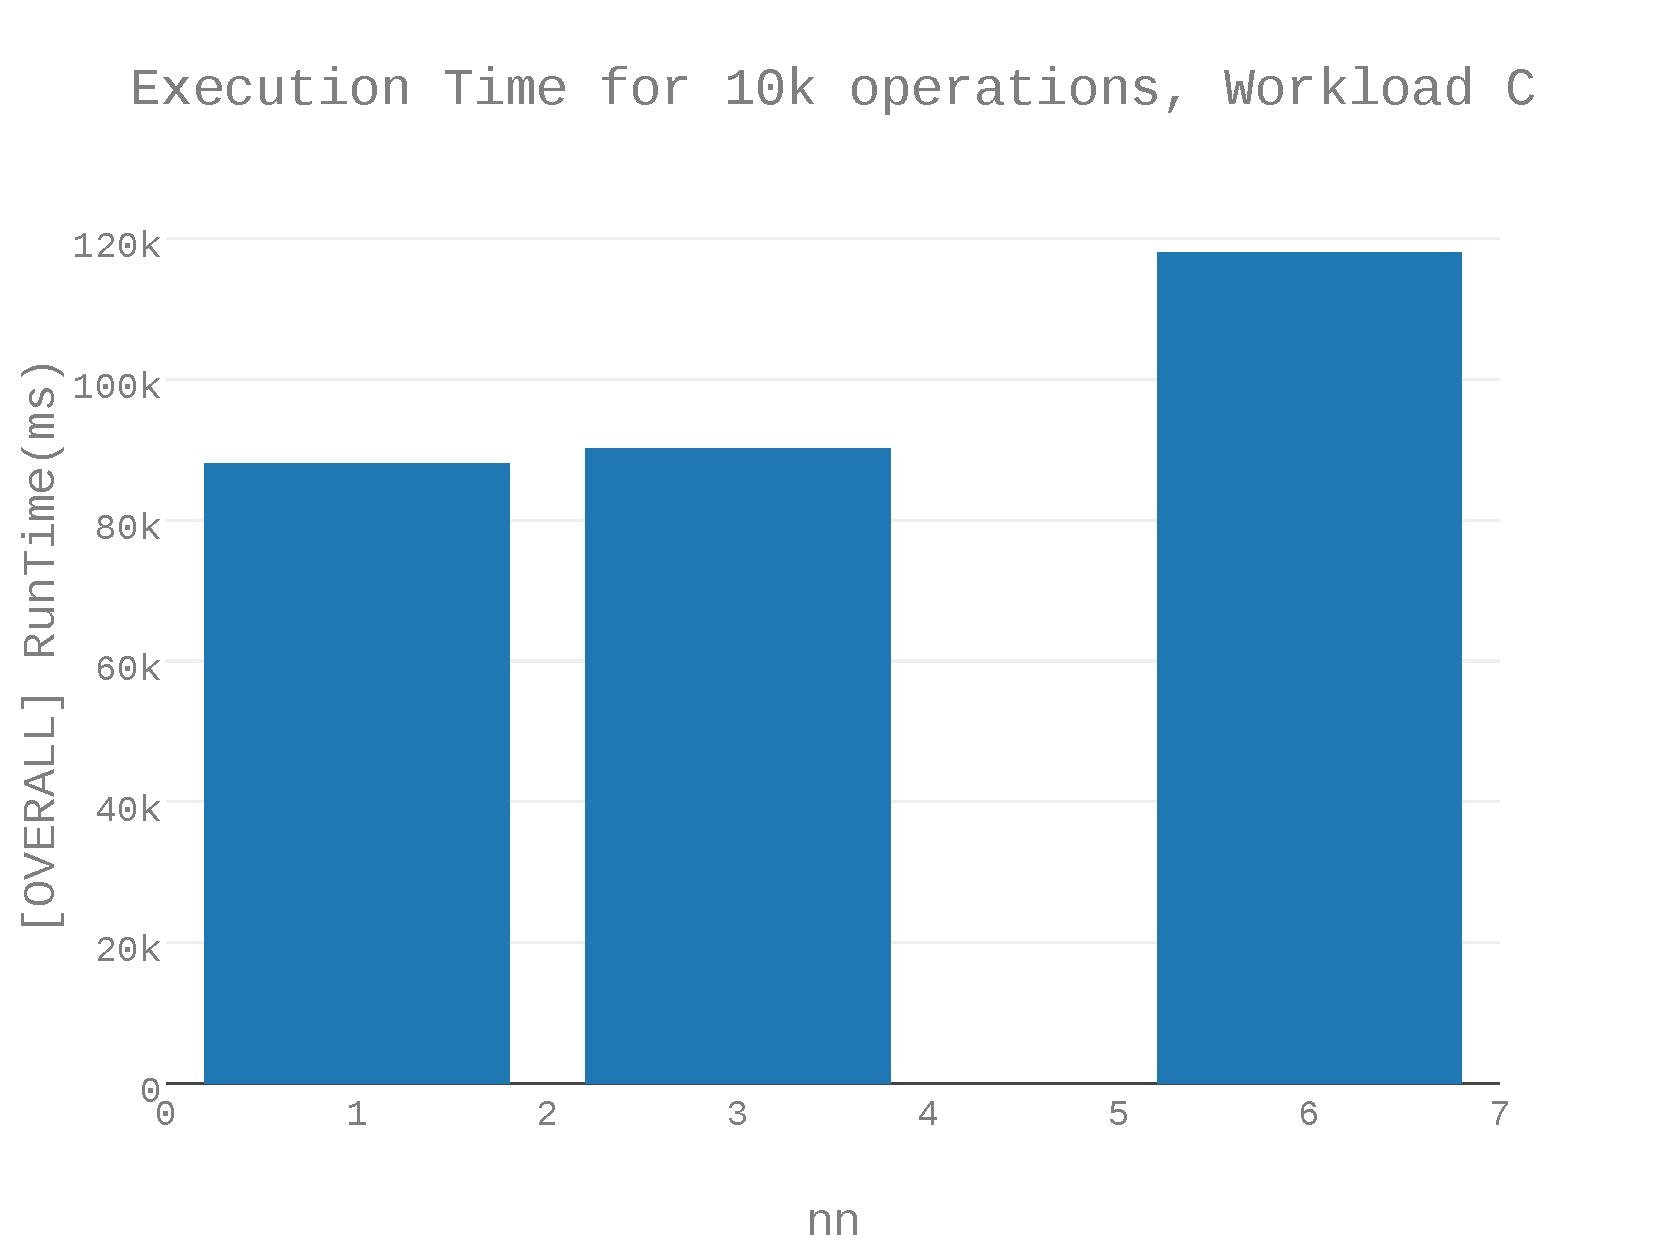
\includegraphics[width=5.5in]{Figures/figures-wlc_fig1.pdf}
\caption{}
\label{figures-wlc_fig1}
\end{figure}

\begin{figure}[h]
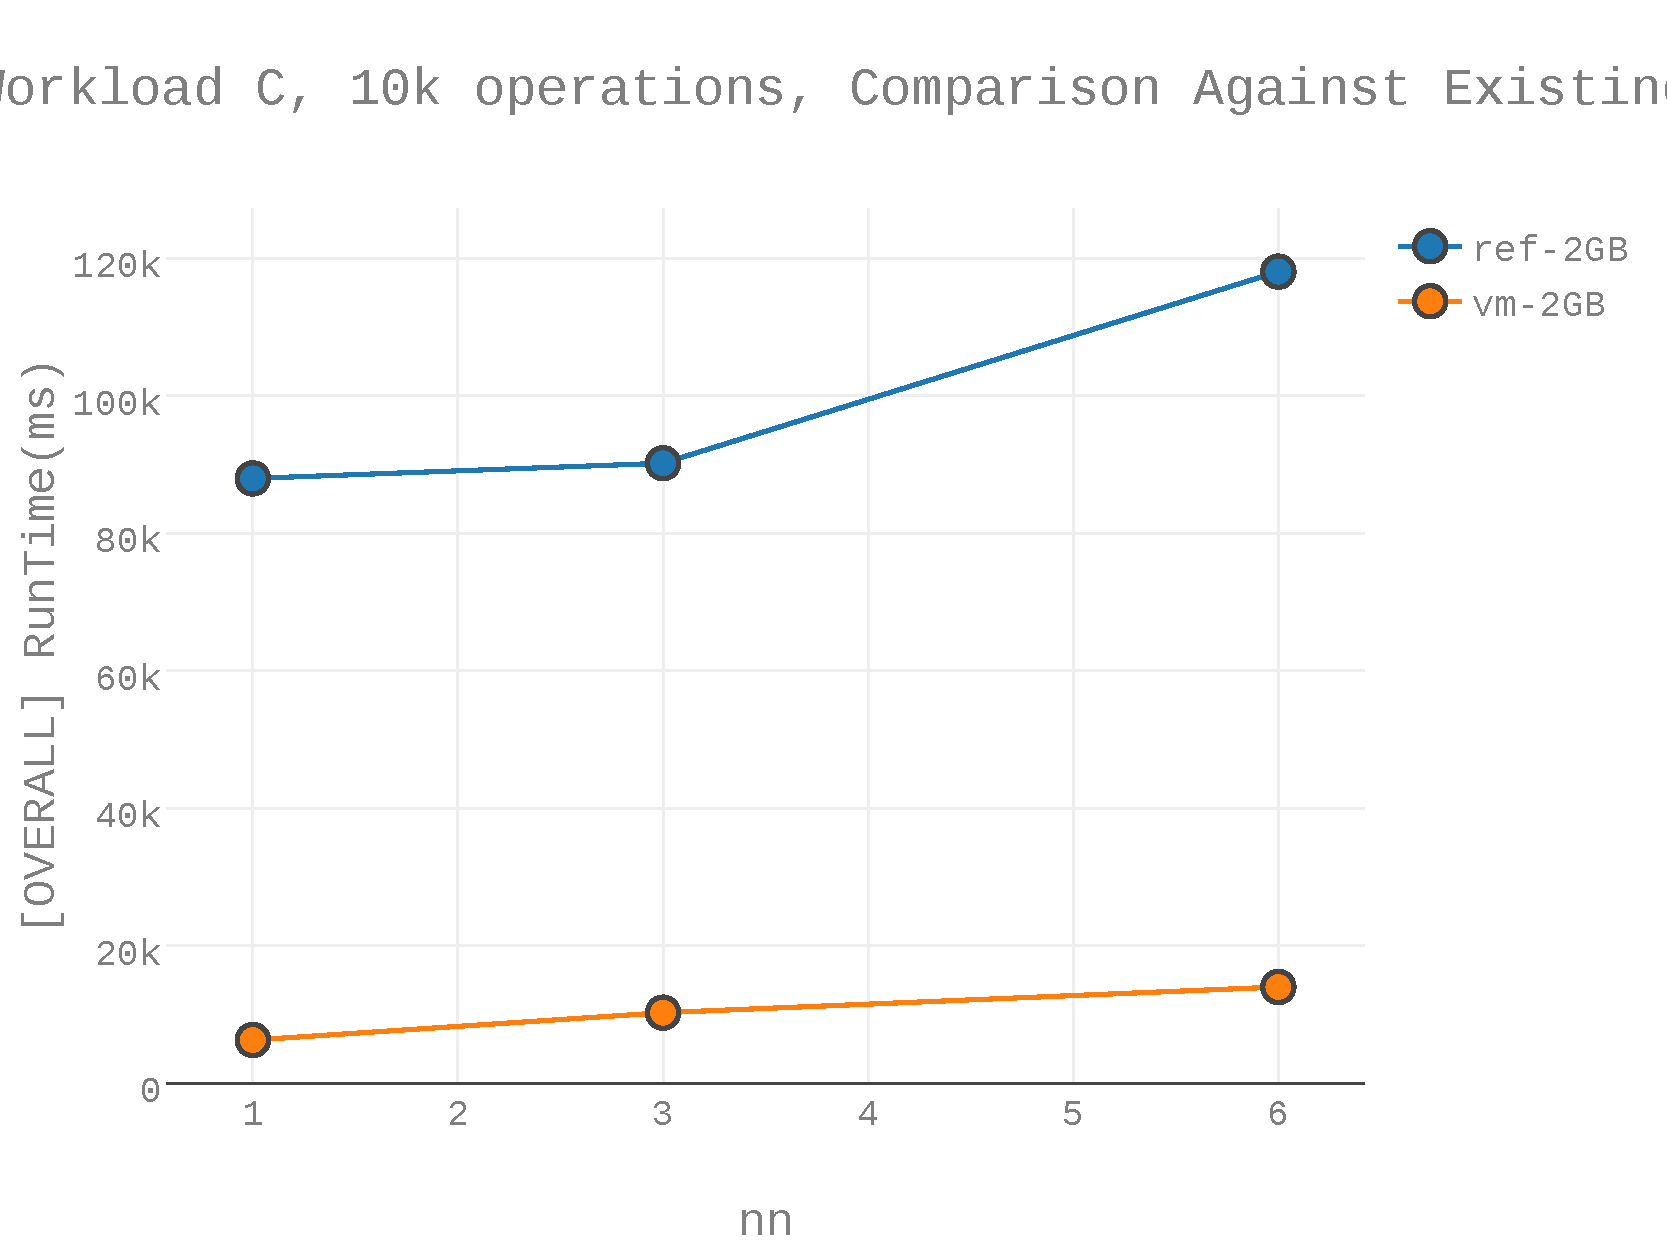
\includegraphics[width=5.5in]{Figures/figures-wlc_fig5.pdf}
\caption{}
\label{figures-wlc_fig5}
\end{figure}



\subsubsection{Ordinal Statistics}
This section will describe some of the summary statistics that describe the data.  

The summary statistics for Workload C performed on the virtual machines are in Tables \ref{table:summary_table_c_1GB_vm_nodal}, \ref{table:summary_table_c_2GB_vm_nodal}, and \ref{table:summary_table_c_4GB_vm_nodal}.
\begin{table}
\begin{tabular}{lrrrr}
\toprule
cluster\_size &     1.0 &     3.0 &     6.0 &  Overall \\
\midrule
25\%   & 6.2e+03 &   1e+04 & 1.4e+04 &  6.3e+03 \\
50\%   & 6.2e+03 &   1e+04 & 1.4e+04 &    1e+04 \\
75\%   & 6.3e+03 &   1e+04 & 1.4e+04 &  1.4e+04 \\
count &      21 &      21 &      21 &       63 \\
max   & 6.9e+03 &   1e+04 & 1.4e+04 &  1.4e+04 \\
mean  & 6.3e+03 &   1e+04 & 1.4e+04 &    1e+04 \\
min   &   6e+03 & 9.8e+03 & 1.3e+04 &    6e+03 \\
range & 9.8e+02 &   6e+02 & 9.8e+02 &  8.5e+03 \\
std   & 2.2e+02 & 1.8e+02 & 2.6e+02 &  3.2e+03 \\
\bottomrule
\end{tabular}
\caption{Summary Statistics for Workload C performed on a 2GB virtual machine node over a(n)nodal network.  Except for count, all values are in milliseconds.}
\label{table:summary_table_c_2GB_vm_nodal}
\end{table}



\subsubsection{Analysis}
This section will take a more in-depth look at the data.
:::something went wrong generating the speedup analysis tables:::

\subsection{1GB RAM vs 2GB RAM vs 4GB RAM}
\subsubsection{Initial Observations}
This section discusses testing and performance for memory sizes: 1GB, 2GB, and 4GB.  The results are displayed in Figure \ref{figures-wlc_fig4}. While it appears the varying the amount of memory has some effect on the results, theredoes not seem to be a predictable pattern across nodes. An ANOVA test will determine if there is an effect, and a linear regression will further testfor an effect. \begin{figure}[h]
\includegraphics[width=5.5in]{Figures/figures-wlc_fig4.pdf}
\caption{}
\label{figures-wlc_fig4}
\end{figure}



\subsubsection{Ordinal Statistics}
This section will describe some of the summary statistics that describe the data.  

The summary statistics for Workload C performed on the virtual machines are in Tables \ref{table:summary_table_c_1GB_vm_nodal}, \ref{table:summary_table_c_2GB_vm_nodal}, and \ref{table:summary_table_c_4GB_vm_nodal}.
\begin{table}
\begin{tabular}{lrrrr}
\toprule
cluster\_size &     1.0 &     3.0 &     6.0 &  Overall \\
\midrule
25\%   & 6.3e+03 & 9.7e+03 & 1.4e+04 &  6.5e+03 \\
50\%   & 6.4e+03 & 9.8e+03 & 1.4e+04 &  9.8e+03 \\
75\%   & 6.5e+03 & 9.9e+03 & 1.5e+04 &  1.4e+04 \\
count &      21 &      21 &      21 &       63 \\
max   & 6.7e+03 & 1.1e+04 & 1.5e+04 &  1.5e+04 \\
mean  & 6.4e+03 & 9.9e+03 & 1.4e+04 &    1e+04 \\
min   & 6.1e+03 & 9.5e+03 & 1.4e+04 &  6.1e+03 \\
range & 6.3e+02 &   1e+03 & 9.8e+02 &  8.9e+03 \\
std   & 1.7e+02 & 2.6e+02 &   3e+02 &  3.3e+03 \\
\bottomrule
\end{tabular}
\caption{Summary Statistics for Workload C performed on a 1GB virtual machine node over a(n)nodal network.  Except for count, all values are in milliseconds.}
\label{table:summary_table_c_1GB_vm_nodal}
\end{table}

\begin{table}
\begin{tabular}{lrrrr}
\toprule
cluster\_size &     1.0 &     3.0 &     6.0 &  Overall \\
\midrule
25\%   &   6e+03 & 9.9e+03 & 1.4e+04 &  6.4e+03 \\
50\%   & 6.1e+03 &   1e+04 & 1.5e+04 &    1e+04 \\
75\%   & 6.4e+03 &   1e+04 & 1.5e+04 &  1.4e+04 \\
count &      21 &      21 &      21 &       63 \\
max   & 6.6e+03 & 1.2e+04 & 1.5e+04 &  1.5e+04 \\
mean  & 6.2e+03 &   1e+04 & 1.5e+04 &    1e+04 \\
min   & 5.9e+03 & 9.8e+03 & 1.4e+04 &  5.9e+03 \\
range & 7.4e+02 & 2.4e+03 & 6.8e+02 &  9.1e+03 \\
std   & 2.3e+02 &   5e+02 & 1.8e+02 &  3.5e+03 \\
\bottomrule
\end{tabular}
\caption{Summary Statistics for Workload C performed on a 4GB virtual machine node over a(n)nodal network.  Except for count, all values are in milliseconds.}
\label{table:summary_table_c_4GB_vm_nodal}
\end{table}




\subsubsection{Analysis}
This section will take a more in-depth look at the data.


\begin{table}[H]
\centering
\begin{tabular}{rrrrrr}
\toprule
 cluster\_size &   slope &  intercept &  r\_value &  p\_value &  std\_err \\
\midrule
            1 &     -71 &    6.4e+03 &    -0.39 &   0.0014 &       21 \\
            3 &   1e+02 &    9.8e+03 &     0.35 &   0.0046 &       35 \\
            6 & 1.1e+02 &    1.4e+04 &     0.36 &   0.0035 &       36 \\
\bottomrule
\end{tabular}
\caption{Linear Regression over amount of RAM}
\label{table:ram_v_ram_c}
\end{table}



\subsection{Implementation on Raspberry Pi}
\subsubsection{Initial Observations}
The results are displayed in Figure \ref{figures-wlc_fig10}.  \begin{figure}[h]
\includegraphics[width=5.5in]{Figures/figures-wlc_fig10.pdf}
\caption{}
\label{figures-wlc_fig10}
\end{figure}



\subsubsection{Ordinal Statistics}
This section will describe some of the summary statistics that describe the data.  

The summary statistics for Workload C performed on the limited hardware, Raspberry Pi, on the Ethernet local area network are in Table \ref{table:summary_table_c_1GB_rp_eth}.
\begin{table}
\begin{tabular}{lrrrrrrr}
\toprule
cluster\_size &     1.0 &     2.0 &     3.0 &     4.0 &     5.0 &     6.0 &  Overall \\
\midrule
25\%   & 4.7e+04 & 1.8e+05 & 1.1e+05 &   1e+05 & 9.7e+04 & 1.1e+05 &  9.8e+04 \\
50\%   & 4.9e+04 & 1.8e+05 & 1.1e+05 &   1e+05 & 9.8e+04 & 1.1e+05 &    1e+05 \\
75\%   &   5e+04 & 1.8e+05 & 1.1e+05 &   1e+05 &   1e+05 & 1.1e+05 &  1.1e+05 \\
count &      21 &      21 &      21 &      21 &      21 &      21 &  1.3e+02 \\
max   &   5e+04 & 1.9e+05 & 1.3e+05 &   1e+05 &   1e+05 & 1.1e+05 &  1.9e+05 \\
mean  & 4.8e+04 & 1.8e+05 & 1.1e+05 &   1e+05 & 9.9e+04 & 1.1e+05 &  1.1e+05 \\
min   & 4.5e+04 & 1.6e+05 & 1.1e+05 &   1e+05 & 9.6e+04 &   1e+05 &  4.5e+04 \\
range & 5.4e+03 & 3.2e+04 & 1.7e+04 &   4e+03 &   7e+03 & 8.1e+03 &  1.5e+05 \\
std   & 1.8e+03 & 6.7e+03 & 3.2e+03 & 1.2e+03 &   2e+03 & 2.1e+03 &  3.9e+04 \\
\bottomrule
\end{tabular}
\caption{Summary Statistics for Workload C performed on a 1GB limited hardware, Raspberry Pi node over a(n)Ethernet network.  Except for count, all values are in milliseconds.}
\label{table:summary_table_c_1GB_rp_eth}
\end{table}



\subsubsection{Analysis}
This section will take a more in-depth look at the data.


\begin{table}[H]
\centering
\begin{tabular}{rrrrr}
\toprule
  slope &  intercept &  r\_value &  p\_value &  std\_err \\
\midrule
1.4e+03 &      1e+05 &     0.06 &      0.5 &    2e+03 \\
\bottomrule
\end{tabular}
\caption{Linear Regression over Cluster Size, Workload c}
\label{table:rp_only_c}
\end{table}



\subsection{Raspberry Pi vs Reference Value}
\subsubsection{Initial Observations}
The results are displayed in Figure \ref{figures-wlc_fig6}.  The performance of the limited hardware, the Raspberry Pi, seems comparable with the results from the more appropriate in the other paper. In addition, there is no reason to suspect a significant differential in the overall pattern with respect to scalability: performance over cluster size. \begin{figure}[h]
\includegraphics[width=5.5in]{Figures/figures-wlc_fig6.pdf}
\caption{}
\label{figures-wlc_fig6}
\end{figure}



\subsubsection{Ordinal Statistics}
This section will describe some of the summary statistics that describe the data.  

The summary statistics for Workload C performed on the limited hardware, Raspberry Pi, on the Ethernet local area network are in Table \ref{table:summary_table_c_1GB_rp_eth}.



\subsubsection{Analysis}
This section will take a more in-depth look at the data.
:::something went wrong generating the speedup analysis tables:::

\subsection{Raspberry Pi vs Virtual Machine}
\subsubsection{Initial Observations}
The results are displayed in Figure \ref{figures-wlc_fig6}.  As expected, there is a significant differential between the limited hardware, the Raspberry Pi configuration and the virtual machine.  However, it is not clear if this is linear across cluster size. 

\subsubsection{Ordinal Statistics}
This section will describe some of the summary statistics that describe the data.  

The summary statistics for Workload C performed on the virtual machines are in Tables \ref{table:summary_table_c_1GB_vm_nodal}, \ref{table:summary_table_c_2GB_vm_nodal}, and \ref{table:summary_table_c_4GB_vm_nodal}.
The summary statistics for Workload C performed on the limited hardware, Raspberry Pi, on the Ethernet local area network are in Table \ref{table:summary_table_c_1GB_rp_eth}.



\subsubsection{Analysis}
This section will take a more in-depth look at the data.




\begin{table}[H]
\centering
\begin{tabular}{lrrrrr}
\toprule
cluster\_size &   slope &  intercept &  r\_value &  p\_value &  std\_err \\
\midrule
           1 & 4.2e+04 &    6.4e+03 &        1 &  1.1e-50 &  3.9e+02 \\
           2 &     nan &        nan &        0 &        1 &      inf \\
           3 &   1e+05 &    9.9e+03 &        1 &  2.4e-56 &    7e+02 \\
           4 &     nan &        nan &        0 &        1 &      inf \\
           5 &     nan &        nan &        0 &        1 &      inf \\
           6 & 9.4e+04 &    1.4e+04 &        1 &  1.2e-61 &  4.7e+02 \\
     OVERALL & 9.8e+04 &      1e+04 &     0.83 &  1.6e-48 &  4.9e+03 \\
\bottomrule
\end{tabular}
\caption{Linear Regression over the effect of limited hardware, Workload C}
\label{table:rp_v_vm_c}
\end{table}





\begin{table}[H]
\centering
\begin{tabular}{llllllll}
\toprule
{} &     0 &    1 &     2 &    3 &    4 &    5 &        6 \\
\midrule
cluster\_size         &     1 &    2 &     3 &    4 &    5 &    6 &  OVERALL \\
ratio\_max\_to\_min     &  0.15 &  NaN & 0.097 &  NaN &  NaN & 0.14 &     0.33 \\
ratio\_min\_to\_max     &  0.12 &  NaN & 0.076 &  NaN &  NaN & 0.12 &    0.032 \\
ratio\_of\_the\_means   &  0.13 &  NaN & 0.087 &  NaN &  NaN & 0.13 &    0.094 \\
ratio\_of\_the\_medians &  0.13 &  NaN & 0.087 &  NaN &  NaN & 0.13 &    0.094 \\
ratio\_of\_the\_stddevs & 0.092 &  NaN & 0.079 &  NaN &  NaN & 0.14 &    0.085 \\
\bottomrule
\end{tabular}
\caption{Speedup over the effect of limited hardware, Workload C}
\label{table:rp_v_vm_c_speedup}
\end{table}





\subsection{Wireless Links Only}
\subsubsection{Initial Observations}
The results are displayed in Figure \ref{figures-wlc_fig8}.  Although there is a general trend of increased execution time over cluster size, the oscillation that occurs between odd and even node cluster sizes is hard to miss. This may be result of the collision avoidance strategy, but further experiments would be needed to determine a more specific explanation. \begin{figure}[h]
\includegraphics[width=5.5in]{Figures/figures-wlc_fig8.pdf}
\caption{}
\label{figures-wlc_fig8}
\end{figure}



\subsubsection{Ordinal Statistics}
This section will describe some of the summary statistics that describe the data.  

The summary statistics for Workload C performed on the limited hardware, Raspberry Pi, on the Ethernet local area network are in Table \ref{table:summary_table_c_1GB_rp_wlan}.
\begin{table}
\begin{tabular}{lrrrrrrr}
\toprule
cluster\_size &     1.0 &     2.0 &     3.0 &     4.0 &     5.0 &     6.0 &  Overall \\
\midrule
25\%   & 6.4e+04 & 1.8e+05 & 1.4e+05 & 2.7e+05 & 1.8e+05 & 2.5e+05 &  1.4e+05 \\
50\%   &   7e+04 & 1.9e+05 & 1.4e+05 & 2.7e+05 & 1.9e+05 & 2.7e+05 &  1.9e+05 \\
75\%   & 8.3e+04 &   2e+05 & 1.4e+05 & 2.8e+05 & 1.9e+05 & 2.9e+05 &  2.6e+05 \\
count &      21 &      21 &      21 &      21 &      21 &      21 &  1.3e+02 \\
max   & 9.4e+04 & 2.2e+05 & 1.9e+05 & 3.1e+05 & 2.4e+05 & 3.1e+05 &  3.1e+05 \\
mean  & 7.3e+04 & 1.9e+05 & 1.4e+05 & 2.8e+05 & 1.9e+05 & 2.7e+05 &  1.9e+05 \\
min   & 5.6e+04 & 1.7e+05 & 1.4e+05 & 2.3e+05 & 1.8e+05 & 2.2e+05 &  5.6e+04 \\
range & 3.8e+04 & 4.8e+04 & 5.5e+04 & 8.3e+04 & 6.2e+04 & 8.3e+04 &  2.6e+05 \\
std   & 1.2e+04 & 1.5e+04 & 1.1e+04 & 1.9e+04 & 1.6e+04 & 2.7e+04 &  7.2e+04 \\
\bottomrule
\end{tabular}
\caption{Summary Statistics for Workload C performed on a 1GB limited hardware, Raspberry Pi node over a(n)802.11a/b/g/n network.  Except for count, all values are in milliseconds.}
\label{table:summary_table_c_1GB_rp_wlan}
\end{table}



\subsubsection{Analysis}
This section will take a more in-depth look at the data.


\begin{table}[H]
\centering
\begin{tabular}{rrrrr}
\toprule
  slope &  intercept &  r\_value &  p\_value &  std\_err \\
\midrule
3.1e+04 &      8e+04 &     0.75 &  6.7e-24 &  2.5e+03 \\
\bottomrule
\end{tabular}
\caption{Linear Regression over Cluster Size, Workload c}
\label{table:wlan_only_c}
\end{table}



\subsection{Wireless Links vs Wired Links}
\subsubsection{Initial Observations}
The results are displayed in Figures \ref{figures-wlc_fig7} and \ref{figures-wlc_fig9}.  For 1, 2, and 3-node clusters, despite the expected  disparity in execution time, the wired and wireless trends seem to follow each other.  However, from 3 nodes up through 6 nodes, the execution times starts to diverge, suggesting that the wireless has a increasing effect as the number of nodes increases. \begin{figure}[h]
\includegraphics[width=5.5in]{Figures/figures-wlc_fig7.pdf}
\caption{}
\label{figures-wlc_fig7}
\end{figure}

\begin{figure}[h]
\includegraphics[width=5.5in]{Figures/figures-wlc_fig9.pdf}
\caption{}
\label{figures-wlc_fig9}
\end{figure}



\subsubsection{Ordinal Statistics}
This section will describe some of the summary statistics that describe the data.  

The summary statistics for Workload C performed on the limited hardware, Raspberry Pi, on the Ethernet local area network are in Table \ref{table:summary_table_c_1GB_rp_eth}.
The summary statistics for Workload C performed on the limited hardware, Raspberry Pi, on the Ethernet local area network are in Table \ref{table:summary_table_c_1GB_rp_wlan}.



\subsubsection{Analysis}
This section will take a more in-depth look at the data.




\begin{table}[H]
\centering
\begin{tabular}{lrrrrr}
\toprule
cluster\_size &   slope &  intercept &  r\_value &  p\_value &  std\_err \\
\midrule
           1 & 2.5e+04 &    4.8e+04 &     0.83 &  1.3e-11 &  2.6e+03 \\
           2 & 1.1e+04 &    1.8e+05 &     0.43 &   0.0049 &  3.7e+03 \\
           3 &   3e+04 &    1.1e+05 &     0.88 &  2.2e-14 &  2.6e+03 \\
           4 & 1.7e+05 &      1e+05 &     0.99 &  2.5e-34 &  4.2e+03 \\
           5 & 9.2e+04 &    9.9e+04 &     0.97 &  2.7e-26 &  3.6e+03 \\
           6 & 1.6e+05 &    1.1e+05 &     0.97 &  7.4e-27 &    6e+03 \\
     OVERALL & 8.1e+04 &    1.1e+05 &     0.58 &    9e-24 &  7.3e+03 \\
\bottomrule
\end{tabular}
\caption{Linear Regression over the effect of 802.11 links, Workload C}
\label{table:wlan_v_eth_c}
\end{table}





\begin{table}[H]
\centering
\begin{tabular}{llllllll}
\toprule
{} &    0 &    1 &    2 &     3 &    4 &     5 &        6 \\
\midrule
cluster\_size         &    1 &    2 &    3 &     4 &    5 &     6 &  OVERALL \\
ratio\_max\_to\_min     & 0.91 &  1.1 & 0.92 &  0.46 & 0.57 &   0.5 &      3.4 \\
ratio\_min\_to\_max     & 0.48 & 0.73 & 0.57 &  0.32 &  0.4 &  0.34 &     0.14 \\
ratio\_of\_the\_means   & 0.66 & 0.94 & 0.79 &  0.37 & 0.52 &  0.41 &     0.57 \\
ratio\_of\_the\_medians & 0.69 & 0.94 &  0.8 &  0.38 & 0.53 &   0.4 &     0.56 \\
ratio\_of\_the\_stddevs & 0.15 & 0.43 & 0.28 & 0.061 & 0.12 & 0.078 &     0.54 \\
\bottomrule
\end{tabular}
\caption{Speedup over the effect of 802.11 links, Workload C}
\label{table:wlan_v_eth_c_speedup}
\end{table}





\section{Results for Workload E}
\subsection{Comparing Existing Work: Virtual Machine vs the Reference Value}
\subsubsection{Initial Observations}
The result medians are displayed in Figure \ref{figures-wle_fig5}.  As expected, the virtual machine results imply much, much less execution time compared to the reference value, presumably accounting for diminished network latency. For the reference value, it seems a higher cluster size seems to imply a cost, but a cost that decreases as the cluster size increases. However,  further analysis would be required to see if this is not just the product of normal variation.  Because of the high contrast, it difficult to reach any initial predictions for virtual machine.  The flat curve may just be an illusion, a minimization of the differences due to the scale of the graph.  \begin{figure}[h]
\includegraphics[width=5.5in]{Figures/figures-wle_fig1.pdf}
\caption{}
\label{figures-wle_fig1}
\end{figure}

\begin{figure}[h]
\includegraphics[width=5.5in]{Figures/figures-wle_fig5.pdf}
\caption{}
\label{figures-wle_fig5}
\end{figure}



\subsubsection{Ordinal Statistics}
This section will describe some of the summary statistics that describe the data.  

The summary statistics for Workload E performed on the virtual machines are in Tables \ref{table:summary_table_e_1GB_vm_nodal}, \ref{table:summary_table_e_2GB_vm_nodal}, and \ref{table:summary_table_e_4GB_vm_nodal}.
\begin{table}
\begin{tabular}{lrrrr}
\toprule
cluster\_size &     1.0 &     3.0 &     6.0 &  Overall \\
\midrule
25\%   & 2.3e+04 & 2.4e+04 & 3.1e+04 &  2.4e+04 \\
50\%   & 2.5e+04 & 2.4e+04 & 3.1e+04 &  2.6e+04 \\
75\%   & 2.6e+04 & 2.5e+04 & 3.2e+04 &  3.1e+04 \\
count &      21 &      21 &      21 &       63 \\
max   & 2.9e+04 & 2.6e+04 & 3.3e+04 &  3.3e+04 \\
mean  & 2.5e+04 & 2.5e+04 & 3.1e+04 &  2.7e+04 \\
min   & 2.1e+04 & 2.3e+04 & 3.1e+04 &  2.1e+04 \\
range &   8e+03 &   3e+03 &   2e+03 &  1.1e+04 \\
std   & 2.2e+03 & 7.5e+02 & 5.3e+02 &  3.5e+03 \\
\bottomrule
\end{tabular}
\caption{Summary Statistics for Workload E performed on a 2GB virtual machine node over a(n)nodal network.  Except for count, all values are in milliseconds.}
\label{table:summary_table_e_2GB_vm_nodal}
\end{table}



\subsubsection{Analysis}
This section will take a more in-depth look at the data.
:::something went wrong generating the speedup analysis tables:::

\subsection{1GB RAM vs 2GB RAM vs 4GB RAM}
\subsubsection{Initial Observations}
The results are displayed in Figure \ref{figures-wle_fig4}.  First of all, the performance for the a one-node cluster differs significantly between 1GB RAM andall other cases.  While this could be some kind of implementation error, it is best not to draw any conclusions fromthis. It would be best to run these tests again, possibly switching the order to eliminate the possible effect of interference or a mix-up of data. That one case aside, the amount of RAM seems to have had an effect on the results, but there doesnot seem to be any predictive relationship that holds true across cluster sizes. \begin{figure}[h]
\includegraphics[width=5.5in]{Figures/figures-wle_fig4.pdf}
\caption{}
\label{figures-wle_fig4}
\end{figure}



\subsubsection{Ordinal Statistics}
This section will describe some of the summary statistics that describe the data.  

The summary statistics for Workload E performed on the virtual machines are in Tables \ref{table:summary_table_e_1GB_vm_nodal}, \ref{table:summary_table_e_2GB_vm_nodal}, and \ref{table:summary_table_e_4GB_vm_nodal}.
\begin{table}
\begin{tabular}{lrrrr}
\toprule
cluster\_size &     1.0 &     3.0 &     6.0 &  Overall \\
\midrule
25\%   & 3.2e+05 & 2.3e+04 & 3.2e+04 &    3e+04 \\
50\%   & 3.5e+05 & 2.3e+04 & 3.2e+04 &  1.7e+05 \\
75\%   & 3.5e+05 & 2.4e+04 & 3.3e+04 &  3.4e+05 \\
count &      42 &      21 &      21 &       84 \\
max   & 3.7e+05 & 2.6e+04 & 3.4e+04 &  3.7e+05 \\
mean  & 3.4e+05 & 2.3e+04 & 3.2e+04 &  1.8e+05 \\
min   & 3.1e+05 & 2.2e+04 & 3.2e+04 &  2.2e+04 \\
range & 5.9e+04 & 4.1e+03 & 2.6e+03 &  3.5e+05 \\
std   & 1.8e+04 &   1e+03 & 6.1e+02 &  1.6e+05 \\
\bottomrule
\end{tabular}
\caption{Summary Statistics for Workload E performed on a 1GB virtual machine node over a(n)nodal network.  Except for count, all values are in milliseconds.}
\label{table:summary_table_e_1GB_vm_nodal}
\end{table}

\begin{table}
\begin{tabular}{lrrrr}
\toprule
cluster\_size &     1.0 &     3.0 &     6.0 &  Overall \\
\midrule
25\%   & 2.4e+04 & 2.3e+04 & 3.3e+04 &  2.4e+04 \\
50\%   & 2.5e+04 & 2.4e+04 & 3.4e+04 &  2.5e+04 \\
75\%   & 2.7e+04 & 2.4e+04 & 3.4e+04 &  3.3e+04 \\
count &      21 &      21 &      21 &       63 \\
max   & 2.8e+04 & 2.8e+04 & 3.5e+04 &  3.5e+04 \\
mean  & 2.5e+04 & 2.4e+04 & 3.4e+04 &  2.8e+04 \\
min   & 1.9e+04 & 2.3e+04 & 3.3e+04 &  1.9e+04 \\
range & 8.4e+03 & 5.6e+03 & 1.9e+03 &  1.5e+04 \\
std   & 2.1e+03 & 1.2e+03 & 6.1e+02 &  4.6e+03 \\
\bottomrule
\end{tabular}
\caption{Summary Statistics for Workload E performed on a 4GB virtual machine node over a(n)nodal network.  Except for count, all values are in milliseconds.}
\label{table:summary_table_e_4GB_vm_nodal}
\end{table}




\subsubsection{Analysis}
This section will take a more in-depth look at the data.


\begin{table}[H]
\centering
\begin{tabular}{rrrrrr}
\toprule
 cluster\_size &    slope &  intercept &  r\_value &  p\_value &  std\_err \\
\midrule
            1 & -1.1e+05 &    3.9e+05 &    -0.81 &    5e-21 &  8.3e+03 \\
            3 &       32 &    2.4e+04 &    0.037 &     0.77 &  1.1e+02 \\
            6 &  4.7e+02 &    3.1e+04 &     0.57 &  1.4e-06 &       88 \\
\bottomrule
\end{tabular}
\caption{Linear Regression over amount of RAM}
\label{table:ram_v_ram_e}
\end{table}



\subsection{Implementation on Raspberry Pi}
\subsubsection{Initial Observations}
The results are displayed in Figure \ref{figures-wle_fig10}.  \begin{figure}[h]
\includegraphics[width=5.5in]{Figures/figures-wle_fig10.pdf}
\caption{}
\label{figures-wle_fig10}
\end{figure}



\subsubsection{Ordinal Statistics}
This section will describe some of the summary statistics that describe the data.  

The summary statistics for Workload E performed on the limited hardware, Raspberry Pi, on the Ethernet local area network are in Table \ref{table:summary_table_e_1GB_rp_eth}.
\begin{table}
\begin{tabular}{lrrrrrrr}
\toprule
cluster\_size &     1.0 &     2.0 &     3.0 &     4.0 &     5.0 &     6.0 &  Overall \\
\midrule
25\%   & 5.2e+05 & 5.2e+05 & 5.1e+05 & 5.3e+05 & 5.4e+05 & 5.6e+05 &  5.2e+05 \\
50\%   & 5.2e+05 & 5.2e+05 & 5.2e+05 & 5.3e+05 & 5.4e+05 & 5.6e+05 &  5.3e+05 \\
75\%   & 5.2e+05 & 5.3e+05 & 5.2e+05 & 5.4e+05 & 5.4e+05 & 5.6e+05 &  5.4e+05 \\
count &      21 &      21 &      21 &      21 &      21 &      21 &  1.3e+02 \\
max   & 5.2e+05 & 5.3e+05 & 5.3e+05 & 5.4e+05 & 5.4e+05 & 5.7e+05 &  5.7e+05 \\
mean  & 5.2e+05 & 5.2e+05 & 5.2e+05 & 5.3e+05 & 5.4e+05 & 5.6e+05 &  5.3e+05 \\
min   & 5.2e+05 & 5.2e+05 & 5.1e+05 & 5.2e+05 & 5.3e+05 & 5.6e+05 &  5.1e+05 \\
range & 8.3e+03 & 1.3e+04 &   2e+04 & 1.8e+04 & 9.9e+03 &   1e+04 &  5.3e+04 \\
std   & 2.1e+03 & 3.5e+03 & 5.5e+03 &   6e+03 & 2.8e+03 &   3e+03 &  1.5e+04 \\
\bottomrule
\end{tabular}
\caption{Summary Statistics for Workload E performed on a 1GB limited hardware, Raspberry Pi node over a(n)Ethernet network.  Except for count, all values are in milliseconds.}
\label{table:summary_table_e_1GB_rp_eth}
\end{table}



\subsubsection{Analysis}
This section will take a more in-depth look at the data.


\begin{table}[H]
\centering
\begin{tabular}{rrrrr}
\toprule
  slope &  intercept &  r\_value &  p\_value &  std\_err \\
\midrule
7.2e+03 &    5.1e+05 &     0.84 &  2.8e-35 &  4.1e+02 \\
\bottomrule
\end{tabular}
\caption{Linear Regression over Cluster Size, Workload e}
\label{table:rp_only_e}
\end{table}



\subsection{Raspberry Pi vs Reference Value}
\subsubsection{Initial Observations}
The results are displayed in Figure \ref{figures-wle_fig6}.  These medians seem to indicate, that for this workload, any effect of the Raspberry Pi is exacerbated with this particular workload. \begin{figure}[h]
\includegraphics[width=5.5in]{Figures/figures-wle_fig6.pdf}
\caption{}
\label{figures-wle_fig6}
\end{figure}



\subsubsection{Ordinal Statistics}
This section will describe some of the summary statistics that describe the data.  

The summary statistics for Workload E performed on the limited hardware, Raspberry Pi, on the Ethernet local area network are in Table \ref{table:summary_table_e_1GB_rp_eth}.



\subsubsection{Analysis}
This section will take a more in-depth look at the data.
:::something went wrong generating the speedup analysis tables:::

\subsection{Raspberry Pi vs Virtual Machine}
\subsubsection{Initial Observations}
The results are displayed in Figure \ref{figures-wle_fig6}.  As expected, there is a significant differential between the limited hardware, the Raspberry Pi configuration and the virtual machine.  However, it is not clear if this is linear across cluster size. 

\subsubsection{Ordinal Statistics}
This section will describe some of the summary statistics that describe the data.  

The summary statistics for Workload E performed on the virtual machines are in Tables \ref{table:summary_table_e_1GB_vm_nodal}, \ref{table:summary_table_e_2GB_vm_nodal}, and \ref{table:summary_table_e_4GB_vm_nodal}.
The summary statistics for Workload E performed on the limited hardware, Raspberry Pi, on the Ethernet local area network are in Table \ref{table:summary_table_e_1GB_rp_eth}.



\subsubsection{Analysis}
This section will take a more in-depth look at the data.




\begin{table}[H]
\centering
\begin{tabular}{lrrrrr}
\toprule
cluster\_size &   slope &  intercept &  r\_value &  p\_value &  std\_err \\
\midrule
           1 & 1.8e+05 &    3.4e+05 &     0.99 &    2e-49 &  3.9e+03 \\
           2 &     nan &        nan &        0 &        1 &      inf \\
           3 &   5e+05 &    2.3e+04 &        1 &  8.9e-74 &  1.2e+03 \\
           4 &     nan &        nan &        0 &        1 &      inf \\
           5 &     nan &        nan &        0 &        1 &      inf \\
           6 & 5.3e+05 &    3.2e+04 &        1 &  1.3e-85 &  6.6e+02 \\
     OVERALL & 3.5e+05 &    1.8e+05 &     0.86 &  1.3e-63 &  1.4e+04 \\
\bottomrule
\end{tabular}
\caption{Linear Regression over the effect of limited hardware, Workload E}
\label{table:rp_v_vm_e}
\end{table}





\begin{table}[H]
\centering
\begin{tabular}{llllllll}
\toprule
{} &    0 &    1 &     2 &    3 &    4 &     5 &        6 \\
\midrule
cluster\_size         &    1 &    2 &     3 &    4 &    5 &     6 &  OVERALL \\
ratio\_max\_to\_min     & 0.72 &  NaN & 0.052 &  NaN &  NaN & 0.061 &     0.72 \\
ratio\_min\_to\_max     &  0.6 &  NaN & 0.042 &  NaN &  NaN & 0.056 &     0.04 \\
ratio\_of\_the\_means   & 0.65 &  NaN & 0.045 &  NaN &  NaN & 0.058 &     0.35 \\
ratio\_of\_the\_medians & 0.66 &  NaN & 0.045 &  NaN &  NaN & 0.058 &     0.33 \\
ratio\_of\_the\_stddevs &  8.4 &  NaN &  0.18 &  NaN &  NaN &  0.21 &       11 \\
\bottomrule
\end{tabular}
\caption{Speedup over the effect of limited hardware, Workload E}
\label{table:rp_v_vm_e_speedup}
\end{table}





\subsection{Wireless Links Only}
\subsubsection{Initial Observations}
The results are displayed in Figure \ref{figures-wle_fig8}.  Although there is a general trend of increased execution time over cluster size, the oscillation that occurs between odd and even node cluster sizes is hard to miss. This may be result of the collision avoidance strategy, but further experiments would be needed to determine a more specific explanation. \begin{figure}[h]
\includegraphics[width=5.5in]{Figures/figures-wle_fig8.pdf}
\caption{}
\label{figures-wle_fig8}
\end{figure}



\subsubsection{Ordinal Statistics}
This section will describe some of the summary statistics that describe the data.  

The summary statistics for Workload E performed on the limited hardware, Raspberry Pi, on the Ethernet local area network are in Table \ref{table:summary_table_e_1GB_rp_wlan}.
\begin{table}
\begin{tabular}{lrrrrrrr}
\toprule
cluster\_size &     1.0 &     2.0 &     3.0 &     4.0 &     5.0 &     6.0 &  Overall \\
\midrule
25\%   & 6.4e+05 & 1.2e+06 & 1.3e+06 & 1.8e+06 & 1.4e+06 & 2.6e+02 &  6.8e+05 \\
50\%   & 6.5e+05 & 1.2e+06 & 1.3e+06 & 1.8e+06 & 1.5e+06 & 2.8e+02 &  1.3e+06 \\
75\%   & 6.6e+05 & 1.3e+06 & 1.3e+06 & 1.9e+06 & 1.5e+06 & 1.8e+06 &  1.6e+06 \\
count &      21 &      21 &      21 &      21 &      21 &      21 &  1.3e+02 \\
max   & 7.2e+05 & 1.9e+06 & 1.5e+06 & 2.5e+06 & 1.6e+06 &   2e+06 &  2.5e+06 \\
mean  & 6.5e+05 & 1.3e+06 & 1.3e+06 & 1.9e+06 & 1.5e+06 & 6.9e+05 &  1.2e+06 \\
min   & 6.3e+05 & 1.1e+06 & 1.2e+06 & 1.7e+06 & 1.4e+06 & 2.6e+02 &  2.6e+02 \\
range & 9.9e+04 &   8e+05 & 2.6e+05 & 7.6e+05 & 2.4e+05 &   2e+06 &  2.5e+06 \\
std   & 2.4e+04 & 2.1e+05 & 6.4e+04 & 1.7e+05 & 6.8e+04 &   9e+05 &  5.8e+05 \\
\bottomrule
\end{tabular}
\caption{Summary Statistics for Workload E performed on a 1GB limited hardware, Raspberry Pi node over a(n)802.11a/b/g/n network.  Except for count, all values are in milliseconds.}
\label{table:summary_table_e_1GB_rp_wlan}
\end{table}



\subsubsection{Analysis}
This section will take a more in-depth look at the data.


\begin{table}[H]
\centering
\begin{tabular}{rrrrr}
\toprule
  slope &  intercept &  r\_value &  p\_value &  std\_err \\
\midrule
4.1e+04 &    1.1e+06 &     0.12 &     0.18 &    3e+04 \\
\bottomrule
\end{tabular}
\caption{Linear Regression over Cluster Size, Workload e}
\label{table:wlan_only_e}
\end{table}



\subsection{Wireless Links vs Wired Links}
\subsubsection{Initial Observations}
The results are displayed in Figures \ref{figures-wle_fig7} and \ref{figures-wle_fig9}.  For 1, 2, and 3-node clusters, despite the expected  disparity in execution time, the wired and wireless trends seem to follow each other.  However, from 3 nodes up through 6 nodes, the execution times starts to diverge, suggesting that the wireless has a increasing effect as the number of nodes increases. \begin{figure}[h]
\includegraphics[width=5.5in]{Figures/figures-wle_fig7.pdf}
\caption{}
\label{figures-wle_fig7}
\end{figure}

\begin{figure}[h]
\includegraphics[width=5.5in]{Figures/figures-wle_fig9.pdf}
\caption{}
\label{figures-wle_fig9}
\end{figure}



\subsubsection{Ordinal Statistics}
This section will describe some of the summary statistics that describe the data.  

The summary statistics for Workload E performed on the limited hardware, Raspberry Pi, on the Ethernet local area network are in Table \ref{table:summary_table_e_1GB_rp_eth}.
The summary statistics for Workload E performed on the limited hardware, Raspberry Pi, on the Ethernet local area network are in Table \ref{table:summary_table_e_1GB_rp_wlan}.



\subsubsection{Analysis}
This section will take a more in-depth look at the data.




\begin{table}[H]
\centering
\begin{tabular}{lrrrrr}
\toprule
cluster\_size &   slope &  intercept &  r\_value &  p\_value &  std\_err \\
\midrule
           1 & 1.3e+05 &    5.2e+05 &     0.97 &    5e-26 &  5.4e+03 \\
           2 & 7.5e+05 &    5.2e+05 &     0.93 &  1.8e-19 &  4.5e+04 \\
           3 & 7.8e+05 &    5.2e+05 &     0.99 &  1.5e-39 &  1.4e+04 \\
           4 & 1.4e+06 &    5.3e+05 &     0.98 &  5.8e-32 &  3.8e+04 \\
           5 & 9.5e+05 &    5.4e+05 &        1 &  5.2e-42 &  1.5e+04 \\
           6 & 1.3e+05 &    5.6e+05 &      0.1 &     0.51 &    2e+05 \\
     OVERALL & 6.8e+05 &    5.3e+05 &     0.64 &    9e-31 &  5.2e+04 \\
\bottomrule
\end{tabular}
\caption{Linear Regression over the effect of 802.11 links, Workload E}
\label{table:wlan_v_eth_e}
\end{table}





\begin{table}[H]
\centering
\begin{tabular}{llllllll}
\toprule
{} &     0 &     1 &     2 &     3 &     4 &       5 &        6 \\
\midrule
cluster\_size         &     1 &     2 &     3 &     4 &     5 &       6 &  OVERALL \\
ratio\_max\_to\_min     &  0.84 &  0.48 &  0.44 &  0.32 &   0.4 & 2.2e+03 &  2.2e+03 \\
ratio\_min\_to\_max     &  0.71 &  0.27 &  0.35 &  0.21 &  0.33 &    0.27 &     0.21 \\
ratio\_of\_the\_means   &   0.8 &  0.41 &   0.4 &  0.28 &  0.36 &    0.81 &     0.44 \\
ratio\_of\_the\_medians &   0.8 &  0.43 &   0.4 &  0.29 &  0.36 &   2e+03 &      0.4 \\
ratio\_of\_the\_stddevs & 0.085 & 0.017 & 0.087 & 0.034 & 0.041 &  0.0033 &    0.025 \\
\bottomrule
\end{tabular}
\caption{Speedup over the effect of 802.11 links, Workload E}
\label{table:wlan_v_eth_e_speedup}
\end{table}





\section{Results for Workload I}
\subsection{1GB RAM vs 2GB RAM vs 4GB RAM}
\subsubsection{Initial Observations}
The results are displayed in Figure \ref{figures-wli_fig4}. Here there is a visible trend of 4GB RAM implying better performance results than both 1GB RAM and 2GB RAM.  However, the relationship between 1GB RAM and 2GB RAM does not seem to be predictable across cluster node sizes. \begin{figure}[h]
\includegraphics[width=5.5in]{Figures/figures-wli_fig4.pdf}
\caption{}
\label{figures-wli_fig4}
\end{figure}



\subsubsection{Ordinal Statistics}
This section will describe some of the summary statistics that describe the data.  

The summary statistics for Workload I performed on the virtual machines are in Tables \ref{table:summary_table_i_1GB_vm_nodal}, \ref{table:summary_table_i_2GB_vm_nodal}, and \ref{table:summary_table_i_4GB_vm_nodal}.
\begin{table}
\begin{tabular}{lrrrrrrr}
\toprule
cluster\_size &     1.0 &     2.0 &     3.0 &     4.0 &     5.0 &     6.0 &  Overall \\
\midrule
25\%   & 9.9e+03 &   1e+04 & 1.3e+04 & 1.4e+04 & 1.9e+04 & 1.4e+04 &  1.3e+04 \\
50\%   &   1e+04 & 1.4e+04 & 1.6e+04 & 1.9e+04 & 2.4e+04 & 1.5e+04 &  1.6e+04 \\
75\%   & 1.5e+04 & 2.2e+04 &   2e+04 & 2.2e+04 & 2.7e+04 & 1.6e+04 &    2e+04 \\
count &      21 &      21 &      21 &      21 &      21 &      21 &  1.3e+02 \\
max   &   2e+04 & 2.3e+04 & 2.6e+04 &   4e+04 & 3.5e+04 & 1.6e+04 &    4e+04 \\
mean  & 1.2e+04 & 1.5e+04 & 1.7e+04 & 1.9e+04 & 2.4e+04 & 1.5e+04 &  1.7e+04 \\
min   & 8.9e+03 & 9.9e+03 & 1.2e+04 & 1.3e+04 & 1.7e+04 & 1.4e+04 &  8.9e+03 \\
range & 1.1e+04 & 1.3e+04 & 1.4e+04 & 2.7e+04 & 1.9e+04 & 1.7e+03 &  3.1e+04 \\
std   & 3.7e+03 & 5.3e+03 & 4.4e+03 & 6.3e+03 & 5.7e+03 & 6.8e+02 &    6e+03 \\
\bottomrule
\end{tabular}
\caption{Summary Statistics for Workload I performed on a 1GB virtual machine node over a(n)nodal network.  Except for count, all values are in milliseconds.}
\label{table:summary_table_i_1GB_vm_nodal}
\end{table}

\begin{table}
\begin{tabular}{lrrrrrrr}
\toprule
cluster\_size &     1.0 &     2.0 &     3.0 &     4.0 &     5.0 &     6.0 &  Overall \\
\midrule
25\%   & 6.5e+03 & 8.8e+03 &   1e+04 & 1.1e+04 & 1.3e+04 & 1.4e+04 &  9.6e+03 \\
50\%   &   7e+03 & 8.9e+03 &   1e+04 & 1.1e+04 & 1.3e+04 & 1.4e+04 &  1.1e+04 \\
75\%   & 1.3e+04 & 8.9e+03 & 1.1e+04 & 1.2e+04 & 1.4e+04 & 1.4e+04 &  1.4e+04 \\
count &      21 &      21 &      21 &      21 &      21 &      21 &  1.3e+02 \\
max   & 2.4e+04 & 9.4e+03 & 1.2e+04 & 1.2e+04 & 1.4e+04 & 1.4e+04 &  2.4e+04 \\
mean  & 1.1e+04 & 8.9e+03 &   1e+04 & 1.1e+04 & 1.3e+04 & 1.4e+04 &  1.2e+04 \\
min   & 6.3e+03 & 8.7e+03 &   1e+04 & 1.1e+04 & 1.3e+04 & 1.4e+04 &  6.3e+03 \\
range & 1.8e+04 & 7.4e+02 & 1.5e+03 & 1.4e+03 & 1.8e+03 & 4.7e+02 &  1.8e+04 \\
std   & 5.7e+03 & 1.5e+02 & 3.6e+02 & 3.6e+02 & 5.5e+02 & 1.4e+02 &  2.9e+03 \\
\bottomrule
\end{tabular}
\caption{Summary Statistics for Workload I performed on a 4GB virtual machine node over a(n)nodal network.  Except for count, all values are in milliseconds.}
\label{table:summary_table_i_4GB_vm_nodal}
\end{table}




\subsubsection{Analysis}
This section will take a more in-depth look at the data.


\begin{table}[H]
\centering
\begin{tabular}{rrrrrr}
\toprule
 cluster\_size &    slope &  intercept &  r\_value &  p\_value &  std\_err \\
\midrule
            1 & -4.7e+02 &    1.3e+04 &    -0.14 &     0.28 &  4.2e+02 \\
            2 & -2.4e+03 &      2e+04 &    -0.49 &    4e-05 &  5.5e+02 \\
            3 & -2.4e+03 &    2.1e+04 &     -0.6 &  2.2e-07 &  4.1e+02 \\
            4 & -2.7e+03 &    2.3e+04 &    -0.62 &  6.7e-08 &  4.4e+02 \\
            5 & -3.5e+03 &    2.7e+04 &    -0.74 &  6.3e-12 &  4.1e+02 \\
            6 & -8.8e+02 &    1.9e+04 &    -0.24 &    0.062 &  4.6e+02 \\
\bottomrule
\end{tabular}
\caption{Linear Regression over amount of RAM}
\label{table:ram_v_ram_i}
\end{table}



\subsection{Implementation on Raspberry Pi}
\subsubsection{Initial Observations}
The results are displayed in Figure \ref{figures-wli_fig10}.  \begin{figure}[h]
\includegraphics[width=5.5in]{Figures/figures-wli_fig10.pdf}
\caption{}
\label{figures-wli_fig10}
\end{figure}



\subsubsection{Ordinal Statistics}
This section will describe some of the summary statistics that describe the data.  

The summary statistics for Workload I performed on the limited hardware, Raspberry Pi, on the Ethernet local area network are in Table \ref{table:summary_table_i_1GB_rp_eth}.
\begin{table}
\begin{tabular}{lrrrrrrr}
\toprule
cluster\_size &     1.0 &     2.0 &     3.0 &     4.0 &     5.0 &     6.0 &  Overall \\
\midrule
25\%   & 4.9e+04 & 1.4e+05 & 1.2e+05 & 1.1e+05 & 1.1e+05 & 1.2e+05 &  1.1e+05 \\
50\%   & 4.9e+04 & 1.4e+05 & 1.2e+05 & 1.1e+05 & 1.1e+05 & 1.2e+05 &  1.2e+05 \\
75\%   &   5e+04 & 1.4e+05 & 1.2e+05 & 1.1e+05 & 1.2e+05 & 1.2e+05 &  1.2e+05 \\
count &      21 &      21 &      21 &      21 &      21 &      21 &  1.3e+02 \\
max   & 5.2e+04 & 1.4e+05 & 1.2e+05 & 1.1e+05 & 1.2e+05 & 1.3e+05 &  1.4e+05 \\
mean  & 4.9e+04 & 1.4e+05 & 1.2e+05 & 1.1e+05 & 1.1e+05 & 1.2e+05 &  1.1e+05 \\
min   & 4.7e+04 & 1.4e+05 & 1.2e+05 & 1.1e+05 & 1.1e+05 & 1.2e+05 &  4.7e+04 \\
range & 4.8e+03 & 4.8e+03 & 3.4e+03 & 3.1e+03 & 7.8e+03 &   8e+03 &  9.6e+04 \\
std   & 9.2e+02 & 1.1e+03 & 9.9e+02 & 7.7e+02 & 2.2e+03 & 2.1e+03 &  2.9e+04 \\
\bottomrule
\end{tabular}
\caption{Summary Statistics for Workload I performed on a 1GB limited hardware, Raspberry Pi node over a(n)Ethernet network.  Except for count, all values are in milliseconds.}
\label{table:summary_table_i_1GB_rp_eth}
\end{table}



\subsubsection{Analysis}
This section will take a more in-depth look at the data.


\begin{table}[H]
\centering
\begin{tabular}{rrrrr}
\toprule
  slope &  intercept &  r\_value &  p\_value &  std\_err \\
\midrule
7.8e+03 &    8.2e+04 &     0.47 &    3e-08 &  1.3e+03 \\
\bottomrule
\end{tabular}
\caption{Linear Regression over Cluster Size, Workload i}
\label{table:rp_only_i}
\end{table}



\subsection{Raspberry Pi vs Virtual Machine}
\subsubsection{Initial Observations}
The results are displayed in Figure \ref{figures-wli_fig6}.  As expected, there is a significant differential between the limited hardware, the Raspberry Pi configuration and the virtual machine.  However, it is not clear if this is linear across cluster size. 

\subsubsection{Ordinal Statistics}
This section will describe some of the summary statistics that describe the data.  

The summary statistics for Workload I performed on the virtual machines are in Tables \ref{table:summary_table_i_1GB_vm_nodal}, \ref{table:summary_table_i_2GB_vm_nodal}, and \ref{table:summary_table_i_4GB_vm_nodal}.
The summary statistics for Workload I performed on the limited hardware, Raspberry Pi, on the Ethernet local area network are in Table \ref{table:summary_table_i_1GB_rp_eth}.



\subsubsection{Analysis}
This section will take a more in-depth look at the data.




\begin{table}[H]
\centering
\begin{tabular}{lrrrrr}
\toprule
cluster\_size &   slope &  intercept &  r\_value &  p\_value &  std\_err \\
\midrule
           1 & 3.7e+04 &    1.2e+04 &     0.99 &  1.1e-35 &  8.3e+02 \\
           2 & 1.3e+05 &    1.5e+04 &        1 &  1.2e-50 &  1.2e+03 \\
           3 &   1e+05 &    1.7e+04 &        1 &  2.1e-50 &  9.8e+02 \\
           4 & 9.2e+04 &    1.9e+04 &        1 &  1.4e-42 &  1.4e+03 \\
           5 & 8.9e+04 &    2.4e+04 &        1 &  9.1e-43 &  1.3e+03 \\
           6 & 1.1e+05 &    1.5e+04 &        1 &  4.8e-63 &  4.9e+02 \\
     OVERALL & 9.2e+04 &    1.7e+04 &     0.91 &  1.7e-99 &  2.6e+03 \\
\bottomrule
\end{tabular}
\caption{Linear Regression over the effect of limited hardware, Workload I}
\label{table:rp_v_vm_i}
\end{table}





\begin{table}[H]
\centering
\begin{tabular}{llllllll}
\toprule
{} &    0 &     1 &    2 &    3 &    4 &    5 &        6 \\
\midrule
cluster\_size         &    1 &     2 &    3 &    4 &    5 &    6 &  OVERALL \\
ratio\_max\_to\_min     & 0.42 &  0.17 & 0.22 & 0.37 & 0.32 & 0.14 &     0.85 \\
ratio\_min\_to\_max     & 0.17 & 0.069 &  0.1 & 0.11 & 0.14 & 0.11 &    0.062 \\
ratio\_of\_the\_means   & 0.25 &  0.11 & 0.14 & 0.17 & 0.21 & 0.12 &     0.16 \\
ratio\_of\_the\_medians & 0.21 & 0.099 & 0.13 & 0.17 & 0.21 & 0.12 &     0.13 \\
ratio\_of\_the\_stddevs &    4 &   4.6 &  4.4 &  8.2 &  2.5 & 0.32 &     0.21 \\
\bottomrule
\end{tabular}
\caption{Speedup over the effect of limited hardware, Workload I}
\label{table:rp_v_vm_i_speedup}
\end{table}





\subsection{Wireless Links Only}
\subsubsection{Initial Observations}
The results are displayed in Figure \ref{figures-wli_fig8}.  There does not seem to be the oscillation that there was in the other workloads, which seems to suggest that somehow the reads and scans that dominate the other workloads are somehow correlated with the oscillation previously observed. Furthermore, this would seem to suggest that Workload I or any similar workload could be used as a control in such an experiment to further investigate the source of the oscillation observed in other, more read-heavy workloads.   As far as the general trend, the results depicted here seem to suggest that at from 3-node clusters on, there seems to be an diminishing increase in execution time as the node cluster increases.  \begin{figure}[h]
\includegraphics[width=5.5in]{Figures/figures-wli_fig8.pdf}
\caption{}
\label{figures-wli_fig8}
\end{figure}



\subsubsection{Ordinal Statistics}
This section will describe some of the summary statistics that describe the data.  

The summary statistics for Workload I performed on the limited hardware, Raspberry Pi, on the Ethernet local area network are in Table \ref{table:summary_table_i_1GB_rp_wlan}.
\begin{table}
\begin{tabular}{lrrrrrrr}
\toprule
cluster\_size &     1.0 &     2.0 &     3.0 &     4.0 &     5.0 &     6.0 &  Overall \\
\midrule
25\%   & 7.6e+04 & 1.7e+05 & 1.3e+05 & 1.7e+05 & 2.3e+05 & 2.4e+05 &  1.5e+05 \\
50\%   & 8.8e+04 & 1.8e+05 & 1.4e+05 & 1.9e+05 & 2.4e+05 & 2.5e+05 &  1.8e+05 \\
75\%   & 1.2e+05 & 1.8e+05 & 1.5e+05 & 1.9e+05 & 2.4e+05 & 2.6e+05 &  2.4e+05 \\
count &      21 &      21 &      21 &      21 &      21 &      21 &  1.3e+02 \\
max   & 2.7e+05 & 1.9e+05 & 1.6e+05 & 2.6e+05 & 3.2e+05 & 2.9e+05 &  3.2e+05 \\
mean  & 1.1e+05 & 1.8e+05 & 1.4e+05 & 1.9e+05 & 2.4e+05 & 2.5e+05 &  1.8e+05 \\
min   & 6.9e+04 & 1.7e+05 & 1.2e+05 & 1.5e+05 & 2.2e+05 & 2.4e+05 &  6.9e+04 \\
range & 2.1e+05 & 2.4e+04 & 4.3e+04 & 1.1e+05 &   1e+05 & 5.4e+04 &  2.6e+05 \\
std   & 4.7e+04 & 6.1e+03 & 1.4e+04 & 2.3e+04 & 2.1e+04 & 1.3e+04 &  5.7e+04 \\
\bottomrule
\end{tabular}
\caption{Summary Statistics for Workload I performed on a 1GB limited hardware, Raspberry Pi node over a(n)802.11a/b/g/n network.  Except for count, all values are in milliseconds.}
\label{table:summary_table_i_1GB_rp_wlan}
\end{table}



\subsubsection{Analysis}
This section will take a more in-depth look at the data.


\begin{table}[H]
\centering
\begin{tabular}{rrrrr}
\toprule
  slope &  intercept &  r\_value &  p\_value &  std\_err \\
\midrule
2.7e+04 &    8.7e+04 &     0.83 &  3.4e-33 &  1.7e+03 \\
\bottomrule
\end{tabular}
\caption{Linear Regression over Cluster Size, Workload i}
\label{table:wlan_only_i}
\end{table}



\subsection{Wireless Links vs Wired Links}
\subsubsection{Initial Observations}
The results are displayed in Figures \ref{figures-wli_fig7} and \ref{figures-wli_fig9}.  For 1, 2, and 3-node clusters, despite the expected  disparity in execution time, the wired and wireless trends seem to follow each other.  However, from 3 nodes up through 6 nodes, the execution times starts to diverge, suggesting that the wireless has a increasing effect as the number of nodes increases. \begin{figure}[h]
\includegraphics[width=5.5in]{Figures/figures-wli_fig7.pdf}
\caption{}
\label{figures-wli_fig7}
\end{figure}

\begin{figure}[h]
\includegraphics[width=5.5in]{Figures/figures-wli_fig9.pdf}
\caption{}
\label{figures-wli_fig9}
\end{figure}



\subsubsection{Ordinal Statistics}
This section will describe some of the summary statistics that describe the data.  

The summary statistics for Workload I performed on the limited hardware, Raspberry Pi, on the Ethernet local area network are in Table \ref{table:summary_table_i_1GB_rp_eth}.
The summary statistics for Workload I performed on the limited hardware, Raspberry Pi, on the Ethernet local area network are in Table \ref{table:summary_table_i_1GB_rp_wlan}.



\subsubsection{Analysis}
This section will take a more in-depth look at the data.




\begin{table}[H]
\centering
\begin{tabular}{lrrrrr}
\toprule
cluster\_size &   slope &  intercept &  r\_value &  p\_value &  std\_err \\
\midrule
           1 & 5.6e+04 &    4.9e+04 &     0.65 &  2.6e-06 &    1e+04 \\
           2 & 3.7e+04 &    1.4e+05 &     0.97 &    2e-27 &  1.3e+03 \\
           3 & 2.1e+04 &    1.2e+05 &     0.74 &  1.8e-08 &    3e+03 \\
           4 & 7.4e+04 &    1.1e+05 &     0.92 &  9.9e-18 &  5.1e+03 \\
           5 & 1.2e+05 &    1.1e+05 &     0.97 &  3.6e-27 &  4.7e+03 \\
           6 & 1.3e+05 &    1.2e+05 &     0.99 &  1.6e-35 &  2.9e+03 \\
     OVERALL & 7.4e+04 &    1.1e+05 &     0.64 &  3.6e-30 &  5.6e+03 \\
\bottomrule
\end{tabular}
\caption{Linear Regression over the effect of 802.11 links, Workload I}
\label{table:wlan_v_eth_i}
\end{table}





\begin{table}[H]
\centering
\begin{tabular}{llllllll}
\toprule
{} &    0 &    1 &     2 &     3 &    4 &    5 &        6 \\
\midrule
cluster\_size         &    1 &    2 &     3 &     4 &    5 &    6 &  OVERALL \\
ratio\_max\_to\_min     & 0.75 & 0.85 &     1 &  0.76 & 0.52 & 0.53 &      2.1 \\
ratio\_min\_to\_max     & 0.17 & 0.72 &  0.72 &  0.43 & 0.34 & 0.41 &     0.15 \\
ratio\_of\_the\_means   & 0.47 & 0.79 &  0.85 &   0.6 & 0.48 & 0.48 &      0.6 \\
ratio\_of\_the\_medians & 0.56 & 0.79 &  0.84 &   0.6 & 0.48 & 0.49 &     0.66 \\
ratio\_of\_the\_stddevs & 0.02 & 0.19 & 0.071 & 0.033 &  0.1 & 0.16 &     0.51 \\
\bottomrule
\end{tabular}
\caption{Speedup over the effect of 802.11 links, Workload I}
\label{table:wlan_v_eth_i_speedup}
\end{table}






\chapter{Conclusion and Future Work}

\section{Conclusion}

One of the selling points of a distributed system, and thus a distributed database, is the option to increase the likelihood of survival of data by spreading nodes geographically.  While servers can and are distributed geographically as well, the light weight of the Raspberry Pi and like devices represents a mobility and flexibility that, in certain contexts, gives these nodes potential competitive advantage over a heavy server-type node.  An open question for an application considering the variance in potential nodes is how the less capable CPU may affect performance.

This work imported some results from \cite{Abramova2014} to form a set of reference points, reference points that for all practical purposes represent a likely candidate platform and network upon which one would nominally use Cassandra.  The fact that the machines in \cite{Abramova2014} were restricted to 2GB was a bonus for this work, as these nodes hinted at getting slightly closer to the lucrative domain of interest: in-situ \gls{iot} storage.  Using these references and some controlled variation within this work, the tests done here can start to paint a picture of what one can expect porting a distributed database like Cassandra to a platform like the Raspberry Pi 2 or 3.  To summarize some of the data collected, this work was able to make the following determinations with respect to the research questions 1 through 4 posed earlier:

\subsection{Research Question 1}

For 21 trials, each consisting of 10,000 operations of workload A (50 percent reads and 50 percent updates)  and performed over 1, 3, and 6-node configurations, the greatest absolute deviation from the reference to the Raspberry Pi configuration was found to be 34851.0 milliseconds, or about 35 second(s). Second, for 10,000 operations of this workload and over 1, 2, 3, 4, 5, and 6-node configurations, the greatest absolute deviation from any given  trial in the wired configuration to an analogous trial using wireless configuration was found to be 367262.0 milliseconds, or about 6.1 minute(s). Third, using this workload and the one-way ANOVA test, it was determined with 95 percent confidence that varying the memory of a device does not necessarily imply a differential in performance.

\subsection{Research Question 2}

For 21 trials, each consisting of 10,000 operations of workload C (100 percent reads)  and performed over 1, 3, and 6-node configurations, the greatest absolute deviation from the reference to the Raspberry Pi configuration was found to be 43025.0 milliseconds, or about 43 second(s). Second, for 10,000 operations of this workload and over 1, 2, 3, 4, 5, and 6-node configurations, the greatest absolute deviation from any given  trial in the wired configuration to an analogous trial using wireless configuration was found to be 211759.0 milliseconds, or about 3.5 minute(s). Third, using this workload and the one-way ANOVA test, it was determined with 95 percent confidence that varying the memory of a device does not necessarily imply a differential in performance.

\subsection{Research Question 3}

For 21 trials, each consisting of 10,000 operations of workload E (100 percent scans)  and performed over 1, 3, and 6-node configurations, the greatest absolute deviation from the reference to the Raspberry Pi configuration was found to be 301019.0 milliseconds, or about 5 minute(s). Second, for 10,000 operations of this workload and over 1, 2, 3, 4, 5, and 6-node configurations, the greatest absolute deviation from any given  trial in the wired configuration to an analogous trial using wireless configuration was found to be 1933941.0 milliseconds, or about 32 minute(s). Third, using this workload and the one-way ANOVA test, it was determined with 95 percent confidence that varying the memory of a device does not necessarily imply a differential in performance.

\subsection{Research Question 4}

For 21 trials, each consisting of 10,000 operations of workload I (99 percent inserts, 1 percent reads) and performed over 1, 3, and 6-node configurations, the greatest absolute deviation from the virtual machine at 1GB to the Raspberry Pi configuration was found to be nan milliseconds, or about nan week(s). Second, for 10,000 operations of this workload and over 1, 2, 3, 4, 5, and 6-node configurations, the greatest absolute deviation from any given  trial in the wired configuration to an analogous trial using wireless configuration was found to be nan milliseconds, or about nan week(s).  Varying the RAM was omitted for Research Question 4.

% \subsubsection{Original Template that Dr. Pecarina Wrote}

% Application developers can expect Cassandra to work in IoT computing platforms. We demonstrated The Yahoo Cloud Benchmark on a Raspberry Pi and determined the following

% 1)      Reduced performance of Workload A is not statistically significant for the reduced memory sizes of IoT like devices
% 2)      When varying platforms, performance for Workload A tracks the performance of the reference paper. For trials perform, reduced performance of Workload A is within 100ms of the reference paper (abramova) for wired implementations.
% 3)      When varying communication method, reduced performance of Workload A is within 100ms of the wired platform test (order of magnitude, no greater than 100\% increase in delay)
 
% Then repeat for Workload C and E to find
% 4)      Reduced performance of Workload C is not statistically significant for the reduced memory sizes of IoT like devices
% 5)      When varying platforms, reduced performance of Workload C is within 100ms of the reference paper (abramova) for wired implementations
% 6)      When varying communication method, reduced performance of Workload C is within 100ms of the wired platform test
% 7)      Reduced performance of Workload E is not statistically significant for the reduced memory sizes of IoT like devices
% 8)      When varying platforms, reduced performance of Workload E is within 100ms of the reference paper (abramova) for wired implementations
% 9)      When varying communication method, reduced performance of Workload E is within 100ms of the wired platform test



\section{Future Work}

\label{Future Work}



As was alluded to in the introduction, this research seeks to support a number of possible future endeavors.


\subsection{Generalized Model}

\subsubsection{Overview/Introduction/Motivation}

Let's say you have a distributed sensor network (thermocouples, radars, pressure sensors or something), and you are already sold on the idea of a distributed database.  It doesn't really have to be Cassandra, but let's say you were already searching for Cassandra research when you came across this report.  The only question is, what kind of nodes do you choose?  There is a lot of hardware out there.  The application in your head narrows this down a bit, and let's further suppose you know you want something that doesn't take a whole lot of space, bringing your attention to the Raspberry Pi series and like devices.

Let's further suppose that after curling up with this document, you've decided the results are enough for you to purchase some Raspberry Pi 2's to handle your database.  Problem solved: Your research phase has ended with this sentence. But, wait. Further suppose that upon logging onto Amazon, you find the Raspberry Pi 2's are out of stock.  Or further suppose both that the stock has depleted, and the devices no longer get manufactured.  Now you have to choose something else.  You might agree on the benefit of having some way to predict performance based on hardware parameters.  That method of prediction would be a mathematical model.

Hold on, you might say, before we get into all this math, what about simulation?  Simulation has its place, naturally, but first of all, the simulator you want may not exist.  But, even if a Google search brings up several options, you have to ask yourself a few questions. How reliable is it?  And can you make the same assumptions about timing?  To what ends are you required to, not to mention willing, to go to verify its utility?  Simulation is certainly not ignored by this paper, however, it is really is just a discrete mathematical model with a lot of computations that comes with its own risks and costs.  The software may be free or affordable, but one must ask, is it really worth your time to learn and to execute, or does an alternative exist?  Sometimes, depending on what you really, truly want to know, you can trade up a small amount of precision or certainty for a dis-proportionally greater amount of your time back.

This generalized mathematical model aims for just that.  The next few paragraphs will propose a relatively simple, generalized model.  It will explain how the results in earlier sections of the report sow the seeds this model, and how future work could refine and develop this model into something more predictive.

\subsubsection{The Model}

This section will describe the model in question: how to define a set of hardware nodes in terms of parameters as well as relationships among them.

Despite the complexities of hardware, this proposition asserts that a node can be abstracted to \gls{ram}, rated \gls{io} speeds, and the processor speed.  The experiments done in this report do not vary these parameters sufficiently to do an empirical model, but they provide a data point as well as a framework for developing other experiments to further refine this model.  This work has already suggested that the amount of memory may not be critical or useful in predicting hardware performance, leaving \gls{io} speeds and processor speed.  This work grouped them all as one.

There has been a lot of work in trying to characterize networks, but really for a model like this, this proposition suggests the network can be characterized by the mean ping team between nodes.

\subsubsection{Experiments that would Refine This Model}

Naturally, trying other databases, like MongoDB, in Cassandra's place is one way to achieve further confidence.  In part, the motivation behind using the \gls{ycsb} was its portability for testing a multitude of distributed database applications.  Although the workloads for Cassandra were varied, and different databases are typically optimized and designed for particular workloads, a different database or databases would increase qualitative confidence that the model can be extended to a database not explicitly tested.

In addition, the absolute values in the results of this work do not necessarily represent Cassandra at its best.  In the interest of replication, default values were used much more often than not.  Cassandra boasts a multitude of parameters with which one can vary in attempt to optimize performance, almost to the point where you are almost guaranteed to be running it sub-optimally without employing a Cassandra expert.

%(CONTRIBUTION 2 –Implement and evaluate target applications using a distributed NoSQL database in IoT)
%5.1          Overview 
\subsection{Wifi Collection, Mapping and Crowd Detection}
                Overview, application purpose
\subsubsection{Data Schema}

\subsubsection{Implementation – WiFiPi prototype}
\subsubsection{Discussion}
%5.3          CBIR
%5.3.1      Data Schema
%5.3.2      Implementation – MSACS
%.3.3      Experimental results
%5%.3.4      Discussion of results
%5.4          Summary of Findings for Applications

\bibliographystyle{IEEEtran}
\bibliography{Mendeley.bib}

\appendix

%% Appendix A

\chapter{Host Machine Hardware Information} % Main appendix title

\label{lshw} % For referencing this appendix elsewhere, use \ref{AppendixA}
%\setstretch{1.0}
The following describes the details of the host machine.
\begin{minted}[breaklines]{text}

daniel@daniel-ThinkPad-W541:~\$ sudo lshw
[sudo] password for daniel: 
daniel-thinkpad-w541      
    description: Notebook
    product: 20EGS25R00 (LENOVO\_MT\_20EG)
    vendor: LENOVO
    version: ThinkPad W541
    serial: MJ0301F4
    width: 64 bits
    capabilities: smbios-2.7 dmi-2.7 vsyscall32
    configuration: administrator\_password=disabled chassis=notebook family=ThinkPad W541 power-on\_password=disabled sku=LENOVO\_MT\_20EG uuid=0114DF39-5754-CB11-BDED-DE35A19757E6
  *-core
       description: Motherboard
       product: 20EGS25R00
       vendor: LENOVO
       physical id: 0
       version: Not Defined
       serial: W1KS58Z11GD
       slot: Not Available
     *-cpu
          description: CPU
          product: Intel(R) Core(TM) i7-4910MQ CPU @ 2.90GHz
          vendor: Intel Corp.
          physical id: 0
          bus info: cpu@0
          version: Intel(R) Core(TM) i7-4910MQ CPU @ 2.90GHz
          serial: None
          slot: CPU Socket - U3E1
          size: 2900MHz
          capacity: 3900MHz
          width: 64 bits
          clock: 100MHz
          capabilities: x86-64 fpu fpu\_exception wp vme de pse tsc msr pae mce cx8 apic sep mtrr pge mca cmov pat pse36 clflush dts acpi mmx fxsr sse sse2 ss ht tm pbe syscall nx pdpe1gb rdtscp constant\_tsc arch\_perfmon pebs bts rep\_good nopl xtopology nonstop\_tsc aperfmperf eagerfpu pni pclmulqdq dtes64 monitor ds\_cpl vmx smx est tm2 ssse3 sdbg fma cx16 xtpr pdcm pcid sse4\_1 sse4\_2 x2apic movbe popcnt tsc\_deadline\_timer aes xsave avx f16c rdrand lahf\_lm abm epb tpr\_shadow vnmi flexpriority ept vpid fsgsbase tsc\_adjust bmi1 avx2 smep bmi2 erms invpcid xsaveopt dtherm ida arat pln pts cpufreq
          configuration: cores=4 enabledcores=4 threads=8
        *-cache:0
             description: L1 cache
             physical id: 2
             slot: L1-Cache
             size: 32KiB
             capacity: 32KiB
             capabilities: asynchronous internal write-back instruction
             configuration: level=1
        *-cache:1
             description: L2 cache
             physical id: 3
             slot: L2-Cache
             size: 256KiB
             capacity: 256KiB
             capabilities: asynchronous internal write-back unified
             configuration: level=2
        *-cache:2
             description: L3 cache
             physical id: 4
             slot: L3-Cache
             size: 8MiB
             capacity: 8MiB
             capabilities: asynchronous internal write-back unified
             configuration: level=3
     *-cache
          description: L1 cache
          physical id: 1
          slot: L1-Cache
          size: 32KiB
          capacity: 32KiB
          capabilities: asynchronous internal write-back data
          configuration: level=1
     *-memory
          description: System Memory
          physical id: 5
          slot: System board or motherboard
          size: 32GiB
        *-bank:0
             description: SODIMM DDR3 Synchronous 1600 MHz (0.6 ns)
             product: M471B1G73QH0-YK0
             vendor: Samsung
             physical id: 0
             serial: 12D86CDE
             slot: ChannelA-DIMM0
             size: 8GiB
             width: 64 bits
             clock: 1600MHz (0.6ns)
        *-bank:1
             description: SODIMM DDR3 Synchronous 1600 MHz (0.6 ns)
             product: M471B1G73QH0-YK0
             vendor: Samsung
             physical id: 1
             serial: 12D86CE2
             slot: ChannelA-DIMM1
             size: 8GiB
             width: 64 bits
             clock: 1600MHz (0.6ns)
        *-bank:2
             description: SODIMM DDR3 Synchronous 1600 MHz (0.6 ns)
             product: M471B1G73QH0-YK0
             vendor: Samsung
             physical id: 2
             serial: 12D84361
             slot: ChannelB-DIMM0
             size: 8GiB
             width: 64 bits
             clock: 1600MHz (0.6ns)
        *-bank:3
             description: SODIMM DDR3 Synchronous 1600 MHz (0.6 ns)
             product: M471B1G73QH0-YK0
             vendor: Samsung
             physical id: 3
             serial: 12D86627
             slot: ChannelB-DIMM1
             size: 8GiB
             width: 64 bits
             clock: 1600MHz (0.6ns)
     *-firmware
          description: BIOS
          vendor: LENOVO
          physical id: 41
          version: GNET71WW (2.19 )
          date: 02/05/2015
          size: 128KiB
          capacity: 11MiB
          capabilities: pci pnp upgrade shadowing cdboot bootselect acpi usb biosbootspecification uefi
     *-pci
          description: Host bridge
          product: Xeon E3-1200 v3/4th Gen Core Processor DRAM Controller
          vendor: Intel Corporation
          physical id: 100
          bus info: pci@0000:00:00.0
          version: 06
          width: 32 bits
          clock: 33MHz
        *-pci:0
             description: PCI bridge
             product: Xeon E3-1200 v3/4th Gen Core Processor PCI Express x16 Controller
             vendor: Intel Corporation
             physical id: 1
             bus info: pci@0000:00:01.0
             version: 06
             width: 32 bits
             clock: 33MHz
             capabilities: pci pm msi pciexpress normal\_decode bus\_master cap\_list
             configuration: driver=pcieport
             resources: irq:26 ioport:4000(size=4096) memory:b0000000-b10fffff ioport:80000000(size=301989888)
           *-display
                description: VGA compatible controller
                product: GK106GLM [Quadro K2100M]
                vendor: NVIDIA Corporation
                physical id: 0
                bus info: pci@0000:01:00.0
                version: a1
                width: 64 bits
                clock: 33MHz
                capabilities: pm msi pciexpress vga\_controller bus\_master cap\_list rom
                configuration: driver=nouveau latency=0
                resources: irq:30 memory:b0000000-b0ffffff memory:80000000-8fffffff memory:90000000-91ffffff ioport:4000(size=128) memory:b1000000-b107ffff
        *-display
             description: VGA compatible controller
             product: 4th Gen Core Processor Integrated Graphics Controller
             vendor: Intel Corporation
             physical id: 2
             bus info: pci@0000:00:02.0
             version: 06
             width: 64 bits
             clock: 33MHz
             capabilities: msi pm vga\_controller bus\_master cap\_list rom
             configuration: driver=i915 latency=0
             resources: irq:31 memory:b1400000-b17fffff memory:a0000000-afffffff ioport:5000(size=64)
        *-multimedia:0
             description: Audio device
             product: Xeon E3-1200 v3/4th Gen Core Processor HD Audio Controller
             vendor: Intel Corporation
             physical id: 3
             bus info: pci@0000:00:03.0
             version: 06
             width: 64 bits
             clock: 33MHz
             capabilities: pm msi pciexpress bus\_master cap\_list
             configuration: driver=snd\_hda\_intel latency=0
             resources: irq:29 memory:b2930000-b2933fff
        *-usb:0
             description: USB controller
             product: 8 Series/C220 Series Chipset Family USB xHCI
             vendor: Intel Corporation
             physical id: 14
             bus info: pci@0000:00:14.0
             version: 04
             width: 64 bits
             clock: 33MHz
             capabilities: pm msi xhci bus\_master cap\_list
             configuration: driver=xhci\_hcd latency=0
             resources: irq:27 memory:b2920000-b292ffff
           *-usbhost:0
                product: xHCI Host Controller
                vendor: Linux 4.4.0-47-generic xhci-hcd
                physical id: 0
                bus info: usb@4
                logical name: usb4
                version: 4.04
                capabilities: usb-3.00
                configuration: driver=hub slots=6 speed=5000Mbit/s
           *-usbhost:1
                product: xHCI Host Controller
                vendor: Linux 4.4.0-47-generic xhci-hcd
                physical id: 1
                bus info: usb@3
                logical name: usb3
                version: 4.04
                capabilities: usb-2.00
                configuration: driver=hub slots=15 speed=480Mbit/s
              *-usb:0 UNCLAIMED
                   description: Smart card reader
                   product: EMV Smartcard Reader
                   vendor: Generic
                   physical id: 5
                   bus info: usb@3:5
                   version: 1.20
                   capabilities: usb-2.01
                   configuration: maxpower=50mA speed=12Mbit/s
              *-usb:1
                   description: Mouse
                   product: USB Optical Mouse
                   vendor: Logitech
                   physical id: 6
                   bus info: usb@3:6
                   version: 72.00
                   capabilities: usb-2.00
                   configuration: driver=usbhid maxpower=100mA speed=2Mbit/s
        *-communication:0
             description: Communication controller
             product: 8 Series/C220 Series Chipset Family MEI Controller \#1
             vendor: Intel Corporation
             physical id: 16
             bus info: pci@0000:00:16.0
             version: 04
             width: 64 bits
             clock: 33MHz
             capabilities: pm msi bus\_master cap\_list
             configuration: driver=mei\_me latency=0
             resources: irq:32 memory:b2939000-b293900f
        *-communication:1
             description: Serial controller
             product: 8 Series/C220 Series Chipset Family KT Controller
             vendor: Intel Corporation
             physical id: 16.3
             bus info: pci@0000:00:16.3
             version: 04
             width: 32 bits
             clock: 66MHz
             capabilities: pm msi 16550 bus\_master cap\_list
             configuration: driver=serial latency=0
             resources: irq:17 ioport:50b0(size=8) memory:b2940000-b2940fff
        *-network
             description: Ethernet interface
             product: Ethernet Connection I217-LM
             vendor: Intel Corporation
             physical id: 19
             bus info: pci@0000:00:19.0
             logical name: eth0
             version: 04
             serial: 54:ee:75:6b:49:34
             capacity: 1Gbit/s
             width: 32 bits
             clock: 33MHz
             capabilities: pm msi bus\_master cap\_list ethernet physical tp 10bt 10bt-fd 100bt 100bt-fd 1000bt-fd autonegotiation
             configuration: autonegotiation=on broadcast=yes driver=e1000e driverversion=3.2.6-k firmware=0.13-3 latency=0 link=no multicast=yes port=twisted pair
             resources: irq:34 memory:b2900000-b291ffff memory:b293f000-b293ffff ioport:5080(size=32)
        *-usb:1
             description: USB controller
             product: 8 Series/C220 Series Chipset Family USB EHCI \#2
             vendor: Intel Corporation
             physical id: 1a
             bus info: pci@0000:00:1a.0
             version: 04
             width: 32 bits
             clock: 33MHz
             capabilities: pm debug ehci bus\_master cap\_list
             configuration: driver=ehci-pci latency=0
             resources: irq:16 memory:b293e000-b293e3ff
           *-usbhost
                product: EHCI Host Controller
                vendor: Linux 4.4.0-47-generic ehci\_hcd
                physical id: 1
                bus info: usb@1
                logical name: usb1
                version: 4.04
                capabilities: usb-2.00
                configuration: driver=hub slots=3 speed=480Mbit/s
              *-usb
                   description: USB hub
                   vendor: Intel Corp.
                   physical id: 1
                   bus info: usb@1:1
                   version: 0.04
                   capabilities: usb-2.00
                   configuration: driver=hub slots=6 speed=480Mbit/s
        *-multimedia:1
             description: Audio device
             product: 8 Series/C220 Series Chipset High Definition Audio Controller
             vendor: Intel Corporation
             physical id: 1b
             bus info: pci@0000:00:1b.0
             version: 04
             width: 64 bits
             clock: 33MHz
             capabilities: pm msi pciexpress bus\_master cap\_list
             configuration: driver=snd\_hda\_intel latency=0
             resources: irq:33 memory:b2934000-b2937fff
        *-pci:1
             description: PCI bridge
             product: 8 Series/C220 Series Chipset Family PCI Express Root Port \#1
             vendor: Intel Corporation
             physical id: 1c
             bus info: pci@0000:00:1c.0
             version: d4
             width: 32 bits
             clock: 33MHz
             capabilities: pci pciexpress msi pm normal\_decode bus\_master cap\_list
             configuration: driver=pcieport
             resources: irq:16
        *-pci:2
             description: PCI bridge
             product: 8 Series/C220 Series Chipset Family PCI Express Root Port \#2
             vendor: Intel Corporation
             physical id: 1c.1
             bus info: pci@0000:00:1c.1
             version: d4
             width: 32 bits
             clock: 33MHz
             capabilities: pci pciexpress msi pm normal\_decode bus\_master cap\_list
             configuration: driver=pcieport
             resources: irq:17 memory:b2800000-b28fffff
           *-network
                description: Wireless interface
                product: Wireless 7260
                vendor: Intel Corporation
                physical id: 0
                bus info: pci@0000:03:00.0
                logical name: wlan0
                version: 83
                serial: a4:c4:94:5d:cb:04
                width: 64 bits
                clock: 33MHz
                capabilities: pm msi pciexpress bus\_master cap\_list ethernet physical wireless
                configuration: broadcast=yes driver=iwlwifi driverversion=4.4.0-47-generic firmware=16.242414.0 ip=192.168.1.75 latency=0 link=yes multicast=yes wireless=IEEE 802.11abgn
                resources: irq:35 memory:b2800000-b2801fff
        *-pci:3
             description: PCI bridge
             product: 8 Series/C220 Series Chipset Family PCI Express Root Port \#3
             vendor: Intel Corporation
             physical id: 1c.2
             bus info: pci@0000:00:1c.2
             version: d4
             width: 32 bits
             clock: 33MHz
             capabilities: pci pciexpress msi pm normal\_decode bus\_master cap\_list
             configuration: driver=pcieport
             resources: irq:18 ioport:3000(size=4096) memory:b2000000-b27fffff ioport:b1800000(size=8388608)
        *-pci:4
             description: PCI bridge
             product: 8 Series/C220 Series Chipset Family PCI Express Root Port \#5
             vendor: Intel Corporation
             physical id: 1c.4
             bus info: pci@0000:00:1c.4
             version: d4
             width: 32 bits
             clock: 33MHz
             capabilities: pci pciexpress msi pm normal\_decode bus\_master cap\_list
             configuration: driver=pcieport
             resources: irq:16 ioport:2000(size=4096) memory:b8000000-ce0fffff ioport:d0000000(size=570425344)
        *-usb:2
             description: USB controller
             product: 8 Series/C220 Series Chipset Family USB EHCI \#1
             vendor: Intel Corporation
             physical id: 1d
             bus info: pci@0000:00:1d.0
             version: 04
             width: 32 bits
             clock: 33MHz
             capabilities: pm debug ehci bus\_master cap\_list
             configuration: driver=ehci-pci latency=0
             resources: irq:23 memory:b293d000-b293d3ff
           *-usbhost
                product: EHCI Host Controller
                vendor: Linux 4.4.0-47-generic ehci\_hcd
                physical id: 1
                bus info: usb@2
                logical name: usb2
                version: 4.04
                capabilities: usb-2.00
                configuration: driver=hub slots=3 speed=480Mbit/s
              *-usb
                   description: USB hub
                   vendor: Intel Corp.
                   physical id: 1
                   bus info: usb@2:1
                   version: 0.04
                   capabilities: usb-2.00
                   configuration: driver=hub slots=8 speed=480Mbit/s
        *-isa
             description: ISA bridge
             product: QM87 Express LPC Controller
             vendor: Intel Corporation
             physical id: 1f
             bus info: pci@0000:00:1f.0
             version: 04
             width: 32 bits
             clock: 33MHz
             capabilities: isa bus\_master cap\_list
             configuration: driver=lpc\_ich latency=0
             resources: irq:0
        *-storage
             description: SATA controller
             product: 8 Series/C220 Series Chipset Family 6-port SATA Controller 1 [AHCI mode]
             vendor: Intel Corporation
             physical id: 1f.2
             bus info: pci@0000:00:1f.2
             version: 04
             width: 32 bits
             clock: 66MHz
             capabilities: storage msi pm ahci\_1.0 bus\_master cap\_list
             configuration: driver=ahci latency=0
             resources: irq:28 ioport:50a8(size=8) ioport:50bc(size=4) ioport:50a0(size=8) ioport:50b8(size=4) ioport:5060(size=32) memory:b293c000-b293c7ff
        *-serial UNCLAIMED
             description: SMBus
             product: 8 Series/C220 Series Chipset Family SMBus Controller
             vendor: Intel Corporation
             physical id: 1f.3
             bus info: pci@0000:00:1f.3
             version: 04
             width: 64 bits
             clock: 33MHz
             configuration: latency=0
             resources: memory:b2938000-b29380ff ioport:efa0(size=32)
     *-scsi:0
          physical id: 2
          logical name: scsi0
          capabilities: emulated
        *-disk
             description: ATA Disk
             product: HGST HTS725050A7
             physical id: 0.0.0
             bus info: scsi@0:0.0.0
             logical name: /dev/sda
             version: B840
             serial: RCE55ACE0VG6PM
             size: 465GiB (500GB)
             capabilities: partitioned partitioned:dos
             configuration: ansiversion=5 logicalsectorsize=512 sectorsize=4096 signature=d28bfe82
           *-volume:0
                description: Windows NTFS volume
                physical id: 1
                bus info: scsi@0:0.0.0,1
                logical name: /dev/sda1
                version: 3.1
                serial: bc9d-71f4
                size: 497MiB
                capacity: 499MiB
                capabilities: primary bootable ntfs initialized
                configuration: clustersize=4096 created=2016-01-14 14:06:03 filesystem=ntfs label=System state=clean
           *-volume:1
                description: Extended partition
                physical id: 3
                bus info: scsi@0:0.0.0,3
                logical name: /dev/sda3
                size: 448GiB
                capacity: 448GiB
                capabilities: primary extended partitioned partitioned:extended
              *-logicalvolume:0
                   description: Linux swap / Solaris partition
                   physical id: 5
                   logical name: /dev/sda5
                   capacity: 31GiB
                   capabilities: nofs
              *-logicalvolume:1
                   description: Linux filesystem partition
                   physical id: 6
                   logical name: /dev/sda6
                   logical name: /
                   capacity: 416GiB
                   configuration: mount.fstype=ext4 mount.options=rw,relatime,errors=remount-ro,data=ordered state=mounted
     *-scsi:1
          physical id: 3
          logical name: scsi5
          capabilities: emulated
        *-cdrom
             description: DVD-RAM writer
             product: DVD-RAM UJ8G2
             vendor: MATSHITA
             physical id: 0.0.0
             bus info: scsi@5:0.0.0
             logical name: /dev/cdrom
             logical name: /dev/cdrw
             logical name: /dev/dvd
             logical name: /dev/dvdrw
             logical name: /dev/sr0
             version: 1.00
             capabilities: removable audio cd-r cd-rw dvd dvd-r dvd-ram
             configuration: ansiversion=5 status=nodisc
  *-battery
       product: Batt Device Name
       vendor: Batt Manufacture
       physical id: 1
       slot: Front
\end{minted}
%\chapter{Virtual Machine Hardware Information} % Main appendix title
{
\setstretch{1.0}

\label{VirtualMachineHardware} % For referencing this appendix elsewhere, use \ref{AppendixA}
\begin{minted}[breaklines]{text}

daniel-virtualbox         
    description: Computer
    product: VirtualBox ()
    vendor: innotek GmbH
    version: 1.2
    serial: 0
    width: 64 bits
    capabilities: smbios-2.5 dmi-2.5 vsyscall32
    configuration: family=Virtual Machine uuid=FF3C111A-93D6-48AC-96E7-E4C5F4006689
  *-core
       description: Motherboard
       product: VirtualBox
       vendor: Oracle Corporation
       physical id: 0
       version: 1.2
       serial: 0
     *-firmware
          description: BIOS
          vendor: innotek GmbH
          physical id: 0
          version: VirtualBox
          date: 12/01/2006
          size: 128KiB
          capabilities: isa pci cdboot bootselect int9keyboard int10video acpi
     *-memory
          description: System memory
          physical id: 1
          size: 993MiB
     *-cpu
          product: Intel(R) Core(TM) i7-4910MQ CPU @ 2.90GHz
          vendor: Intel Corp.
          physical id: 2
          bus info: cpu@0
          width: 64 bits
          capabilities: fpu fpu_exception wp vme de pse tsc msr pae mce cx8 apic sep mtrr pge mca cmov pat pse36 clflush mmx fxsr sse sse2 syscall nx rdtscp x86-64 constant_tsc rep_good nopl xtopology nonstop_tsc pni pclmulqdq monitor ssse3 cx16 sse4_1 sse4_2 movbe popcnt aes xsave avx rdrand lahf_lm abm
     *-pci
          description: Host bridge
          product: 440FX - 82441FX PMC [Natoma]
          vendor: Intel Corporation
          physical id: 100
          bus info: pci@0000:00:00.0
          version: 02
          width: 32 bits
          clock: 33MHz
        *-isa
             description: ISA bridge
             product: 82371SB PIIX3 ISA [Natoma/Triton II]
             vendor: Intel Corporation
             physical id: 1
             bus info: pci@0000:00:01.0
             version: 00
             width: 32 bits
             clock: 33MHz
             capabilities: isa bus_master
             configuration: latency=0
        *-ide
             description: IDE interface
             product: 82371AB/EB/MB PIIX4 IDE
             vendor: Intel Corporation
             physical id: 1.1
             bus info: pci@0000:00:01.1
             version: 01
             width: 32 bits
             clock: 33MHz
             capabilities: ide bus_master
             configuration: driver=ata_piix latency=64
             resources: irq:0 ioport:1f0(size=8) ioport:3f6 ioport:170(size=8) ioport:376 ioport:d000(size=16)
        *-display
             description: VGA compatible controller
             product: VirtualBox Graphics Adapter
             vendor: InnoTek Systemberatung GmbH
             physical id: 2
             bus info: pci@0000:00:02.0
             version: 00
             width: 32 bits
             clock: 33MHz
             capabilities: vga_controller bus_master rom
             configuration: driver=vboxvideo latency=0
             resources: irq:18 memory:e0000000-e0ffffff
        *-network:0
             description: Ethernet interface
             product: 82540EM Gigabit Ethernet Controller
             vendor: Intel Corporation
             physical id: 3
             bus info: pci@0000:00:03.0
             logical name: eth0
             version: 02
             serial: 08:00:27:a8:77:90
             size: 1Gbit/s
             capacity: 1Gbit/s
             width: 32 bits
             clock: 66MHz
             capabilities: pm pcix bus_master cap_list ethernet physical tp 10bt 10bt-fd 100bt 100bt-fd 1000bt-fd autonegotiation
             configuration: autonegotiation=on broadcast=yes driver=e1000 driverversion=7.3.21-k8-NAPI duplex=full ip=192.168.1.70 latency=64 link=yes mingnt=255 multicast=yes port=twisted pair speed=1Gbit/s
             resources: irq:19 memory:f0000000-f001ffff ioport:d010(size=8)
        *-generic
             description: System peripheral
             product: VirtualBox Guest Service
             vendor: InnoTek Systemberatung GmbH
             physical id: 4
             bus info: pci@0000:00:04.0
             version: 00
             width: 32 bits
             clock: 33MHz
             capabilities: bus_master
             configuration: driver=vboxguest latency=0
             resources: irq:20 ioport:d020(size=32) memory:f0400000-f07fffff memory:f0800000-f0803fff
        *-multimedia
             description: Multimedia audio controller
             product: 82801AA AC'97 Audio Controller
             vendor: Intel Corporation
             physical id: 5
             bus info: pci@0000:00:05.0
             version: 01
             width: 32 bits
             clock: 33MHz
             capabilities: bus_master
             configuration: driver=snd_intel8x0 latency=64
             resources: irq:21 ioport:d100(size=256) ioport:d200(size=64)
        *-usb
             description: USB controller
             product: KeyLargo/Intrepid USB
             vendor: Apple Inc.
             physical id: 6
             bus info: pci@0000:00:06.0
             version: 00
             width: 32 bits
             clock: 33MHz
             capabilities: ohci bus_master cap_list
             configuration: driver=ohci-pci latency=64
             resources: irq:22 memory:f0804000-f0804fff
        *-bridge UNCLAIMED
             description: Bridge
             product: 82371AB/EB/MB PIIX4 ACPI
             vendor: Intel Corporation
             physical id: 7
             bus info: pci@0000:00:07.0
             version: 08
             width: 32 bits
             clock: 33MHz
             capabilities: bridge bus_master
             configuration: latency=0
        *-network:1
             description: Ethernet interface
             product: 82540EM Gigabit Ethernet Controller
             vendor: Intel Corporation
             physical id: 8
             bus info: pci@0000:00:08.0
             logical name: eth1
             version: 02
             serial: 08:00:27:55:2f:10
             size: 1Gbit/s
             capacity: 1Gbit/s
             width: 32 bits
             clock: 66MHz
             capabilities: pm pcix bus_master cap_list ethernet physical tp 10bt 10bt-fd 100bt 100bt-fd 1000bt-fd autonegotiation
             configuration: autonegotiation=on broadcast=yes driver=e1000 driverversion=7.3.21-k8-NAPI duplex=full ip=192.168.56.100 latency=64 link=yes mingnt=255 multicast=yes port=twisted pair speed=1Gbit/s
             resources: irq:16 memory:f0820000-f083ffff ioport:d240(size=8)
        *-storage
             description: SATA controller
             product: 82801HM/HEM (ICH8M/ICH8M-E) SATA Controller [AHCI mode]
             vendor: Intel Corporation
             physical id: d
             bus info: pci@0000:00:0d.0
             version: 02
             width: 32 bits
             clock: 33MHz
             capabilities: storage pm ahci_1.0 bus_master cap_list
             configuration: driver=ahci latency=64
             resources: irq:21 ioport:d248(size=8) ioport:d258(size=8) ioport:d270(size=16) memory:f0840000-f0841fff
     *-scsi:0
          physical id: 3
          logical name: scsi0
          capabilities: emulated
        *-cdrom
             description: DVD reader
             physical id: 0.0.0
             bus info: scsi@0:0.0.0
             logical name: /dev/cdrom
             logical name: /dev/sr0
             logical name: /media/daniel/VBOXADDITIONS_5.0.24_108355
             capabilities: audio dvd
             configuration: mount.fstype=iso9660 mount.options=ro,nosuid,nodev,relatime,uid=1000,gid=1000,iocharset=utf8,mode=0400,dmode=0500 state=mounted status=ready
     *-scsi:1
          physical id: 4
          logical name: scsi1
          capabilities: emulated
        *-cdrom
             description: DVD reader
             physical id: 0.0.0
             bus info: scsi@1:0.0.0
             logical name: /dev/sr1
             capabilities: audio dvd
             configuration: status=nodisc
     *-scsi:2
          physical id: 5
          logical name: scsi2
          capabilities: emulated
        *-disk
             description: ATA Disk
             product: VBOX HARDDISK
             physical id: 0.0.0
             bus info: scsi@2:0.0.0
             logical name: /dev/sda
             version: 1.0
             serial: VBab319aa0-945b328a
             size: 8GiB (8589MB)
             capabilities: partitioned partitioned:dos
             configuration: ansiversion=5 sectorsize=512 signature=0003ba0a
           *-volume:0
                description: EXT4 volume
                vendor: Linux
                physical id: 1
                bus info: scsi@2:0.0.0,1
                logical name: /dev/sda1
                logical name: /
                version: 1.0
                serial: 6df40e27-ba83-4d69-9d66-7f0c60d6ed7b
                size: 7679MiB
                capacity: 7679MiB
                capabilities: primary bootable journaled extended_attributes large_files huge_files dir_nlink recover extents ext4 ext2 initialized
                configuration: created=2016-08-21 17:42:59 filesystem=ext4 lastmountpoint=/ modified=2016-11-23 17:35:01 mount.fstype=ext4 mount.options=rw,relatime,errors=remount-ro,data=ordered mounted=2016-11-23 17:35:01 state=mounted
           *-volume:1
                description: Extended partition
                physical id: 2
                bus info: scsi@2:0.0.0,2
                logical name: /dev/sda2
                size: 510MiB
                capacity: 510MiB
                capabilities: primary extended partitioned partitioned:extended
              *-logicalvolume
                   description: Linux swap / Solaris partition
                   physical id: 5
                   logical name: /dev/sda5
                   capacity: 510MiB
                   capabilities: nofs
\end{minted}
}
%% Appendix Template

\chapter{Cassandra Configuration File} % Main appendix title

\label{Appendix_CassandraConfigurationFile} 

\setstretch{1.0}
The following describes the details of Cassandra's configuration for these tests.
\begin{minted}[breaklines]{text}
# Cassandra storage config YAML 

# NOTE:
#   See http://wiki.apache.org/cassandra/StorageConfiguration for
#   full explanations of configuration directives
# /NOTE

# The name of the cluster. This is mainly used to prevent machines in
# one logical cluster from joining another.
cluster_name: 'Test Cluster'

# This defines the number of tokens randomly assigned to this node on the ring
# The more tokens, relative to other nodes, the larger the proportion of data
# that this node will store. You probably want all nodes to have the same number
# of tokens assuming they have equal hardware capability.
#
# If you leave this unspecified, Cassandra will use the default of 1 token for legacy compatibility,
# and will use the initial_token as described below.
#
# Specifying initial_token will override this setting on the node's initial start,
# on subsequent starts, this setting will apply even if initial token is set.
#
# If you already have a cluster with 1 token per node, and wish to migrate to 
# multiple tokens per node, see http://wiki.apache.org/cassandra/Operations
num_tokens: 256

# Triggers automatic allocation of num_tokens tokens for this node. The allocation
# algorithm attempts to choose tokens in a way that optimizes replicated load over
# the nodes in the datacenter for the replication strategy used by the specified
# keyspace.
#
# The load assigned to each node will be close to proportional to its number of
# vnodes.
#
# Only supported with the Murmur3Partitioner.
# allocate_tokens_for_keyspace: KEYSPACE

# initial_token allows you to specify tokens manually.  While you can use # it with
# vnodes (num_tokens > 1, above) -- in which case you should provide a 
# comma-separated list -- it's primarily used when adding nodes # to legacy clusters 
# that do not have vnodes enabled.
# initial_token:

# See http://wiki.apache.org/cassandra/HintedHandoff
# May either be "true" or "false" to enable globally
hinted_handoff_enabled: true
# When hinted_handoff_enabled is true, a black list of data centers that will not
# perform hinted handoff
#hinted_handoff_disabled_datacenters:
#    - DC1
#    - DC2
# this defines the maximum amount of time a dead host will have hints
# generated.  After it has been dead this long, new hints for it will not be
# created until it has been seen alive and gone down again.
max_hint_window_in_ms: 10800000 # 3 hours

# Maximum throttle in KBs per second, per delivery thread.  This will be
# reduced proportionally to the number of nodes in the cluster.  (If there
# are two nodes in the cluster, each delivery thread will use the maximum
# rate; if there are three, each will throttle to half of the maximum,
# since we expect two nodes to be delivering hints simultaneously.)
hinted_handoff_throttle_in_kb: 1024

# Number of threads with which to deliver hints;
# Consider increasing this number when you have multi-dc deployments, since
# cross-dc handoff tends to be slower
max_hints_delivery_threads: 2

# Directory where Cassandra should store hints.
# If not set, the default directory is $CASSANDRA_HOME/data/hints.
# hints_directory: /var/lib/cassandra/hints

# How often hints should be flushed from the internal buffers to disk.
# Will *not* trigger fsync.
hints_flush_period_in_ms: 10000

# Maximum size for a single hints file, in megabytes.
max_hints_file_size_in_mb: 128

# Compression to apply to the hint files. If omitted, hints files
# will be written uncompressed. LZ4, Snappy, and Deflate compressors
# are supported.
#hints_compression:
#   - class_name: LZ4Compressor
#     parameters:
#         -

# Maximum throttle in KBs per second, total. This will be
# reduced proportionally to the number of nodes in the cluster.
batchlog_replay_throttle_in_kb: 1024

# Authentication backend, implementing IAuthenticator; used to identify users
# Out of the box, Cassandra provides org.apache.cassandra.auth.{AllowAllAuthenticator,
# PasswordAuthenticator}.
#
# - AllowAllAuthenticator performs no checks - set it to disable authentication.
# - PasswordAuthenticator relies on username/password pairs to authenticate
#   users. It keeps usernames and hashed passwords in system_auth.credentials table.
#   Please increase system_auth keyspace replication factor if you use this authenticator.
#   If using PasswordAuthenticator, CassandraRoleManager must also be used (see below)
authenticator: AllowAllAuthenticator

# Authorization backend, implementing IAuthorizer; used to limit access/provide permissions
# Out of the box, Cassandra provides org.apache.cassandra.auth.{AllowAllAuthorizer,
# CassandraAuthorizer}.
#
# - AllowAllAuthorizer allows any action to any user - set it to disable authorization.
# - CassandraAuthorizer stores permissions in system_auth.permissions table. Please
#   increase system_auth keyspace replication factor if you use this authorizer.
authorizer: AllowAllAuthorizer

# Part of the Authentication & Authorization backend, implementing IRoleManager; used
# to maintain grants and memberships between roles.
# Out of the box, Cassandra provides org.apache.cassandra.auth.CassandraRoleManager,
# which stores role information in the system_auth keyspace. Most functions of the
# IRoleManager require an authenticated login, so unless the configured IAuthenticator
# actually implements authentication, most of this functionality will be unavailable.
#
# - CassandraRoleManager stores role data in the system_auth keyspace. Please
#   increase system_auth keyspace replication factor if you use this role manager.
role_manager: CassandraRoleManager

# Validity period for roles cache (fetching permissions can be an
# expensive operation depending on the authorizer). Granted roles are cached for
# authenticated sessions in AuthenticatedUser and after the period specified
# here, become eligible for (async) reload.
# Defaults to 2000, set to 0 to disable.
# Will be disabled automatically for AllowAllAuthenticator.
roles_validity_in_ms: 2000

# Refresh interval for roles cache (if enabled).
# After this interval, cache entries become eligible for refresh. Upon next
# access, an async reload is scheduled and the old value returned until it
# completes. If roles_validity_in_ms is non-zero, then this must be
# also.
# Defaults to the same value as roles_validity_in_ms.
# roles_update_interval_in_ms: 1000

# Validity period for permissions cache (fetching permissions can be an
# expensive operation depending on the authorizer, CassandraAuthorizer is
# one example). Defaults to 2000, set to 0 to disable.
# Will be disabled automatically for AllowAllAuthorizer.
permissions_validity_in_ms: 2000

# Refresh interval for permissions cache (if enabled).
# After this interval, cache entries become eligible for refresh. Upon next
# access, an async reload is scheduled and the old value returned until it
# completes. If permissions_validity_in_ms is non-zero, then this must be
# also.
# Defaults to the same value as permissions_validity_in_ms.
# permissions_update_interval_in_ms: 1000

# The partitioner is responsible for distributing groups of rows (by
# partition key) across nodes in the cluster.  You should leave this
# alone for new clusters.  The partitioner can NOT be changed without
# reloading all data, so when upgrading you should set this to the
# same partitioner you were already using.
#
# Besides Murmur3Partitioner, partitioners included for backwards
# compatibility include RandomPartitioner, ByteOrderedPartitioner, and
# OrderPreservingPartitioner.
#
partitioner: org.apache.cassandra.dht.Murmur3Partitioner

# Directories where Cassandra should store data on disk.  Cassandra
# will spread data evenly across them, subject to the granularity of
# the configured compaction strategy.
# If not set, the default directory is $CASSANDRA_HOME/data/data.
# data_file_directories:
#     - /var/lib/cassandra/data

# commit log.  when running on magnetic HDD, this should be a
# separate spindle than the data directories.
# If not set, the default directory is $CASSANDRA_HOME/data/commitlog.
# commitlog_directory: /var/lib/cassandra/commitlog

# policy for data disk failures:
# die: shut down gossip and client transports and kill the JVM for any fs errors or
#      single-sstable errors, so the node can be replaced.
# stop_paranoid: shut down gossip and client transports even for single-sstable errors,
#                kill the JVM for errors during startup.
# stop: shut down gossip and client transports, leaving the node effectively dead, but
#       can still be inspected via JMX, kill the JVM for errors during startup.
# best_effort: stop using the failed disk and respond to requests based on
#              remaining available sstables.  This means you WILL see obsolete
#              data at CL.ONE!
# ignore: ignore fatal errors and let requests fail, as in pre-1.2 Cassandra
disk_failure_policy: stop

# policy for commit disk failures:
# die: shut down gossip and Thrift and kill the JVM, so the node can be replaced.
# stop: shut down gossip and Thrift, leaving the node effectively dead, but
#       can still be inspected via JMX.
# stop_commit: shutdown the commit log, letting writes collect but
#              continuing to service reads, as in pre-2.0.5 Cassandra
# ignore: ignore fatal errors and let the batches fail
commit_failure_policy: stop

# Maximum size of the key cache in memory.
#
# Each key cache hit saves 1 seek and each row cache hit saves 2 seeks at the
# minimum, sometimes more. The key cache is fairly tiny for the amount of
# time it saves, so it's worthwhile to use it at large numbers.
# The row cache saves even more time, but must contain the entire row,
# so it is extremely space-intensive. It's best to only use the
# row cache if you have hot rows or static rows.
#
# NOTE: if you reduce the size, you may not get you hottest keys loaded on startup.
#
# Default value is empty to make it "auto" (min(5% of Heap (in MB), 100MB)). Set to 0 to disable key cache.
key_cache_size_in_mb:

# Duration in seconds after which Cassandra should
# save the key cache. Caches are saved to saved_caches_directory as
# specified in this configuration file.
#
# Saved caches greatly improve cold-start speeds, and is relatively cheap in
# terms of I/O for the key cache. Row cache saving is much more expensive and
# has limited use.
#
# Default is 14400 or 4 hours.
key_cache_save_period: 14400

# Number of keys from the key cache to save
# Disabled by default, meaning all keys are going to be saved
# key_cache_keys_to_save: 100

# Row cache implementation class name.
# Available implementations:
#   org.apache.cassandra.cache.OHCProvider                Fully off-heap row cache implementation (default).
#   org.apache.cassandra.cache.SerializingCacheProvider   This is the row cache implementation availabile
#                                                         in previous releases of Cassandra.
# row_cache_class_name: org.apache.cassandra.cache.OHCProvider

# Maximum size of the row cache in memory.
# Please note that OHC cache implementation requires some additional off-heap memory to manage
# the map structures and some in-flight memory during operations before/after cache entries can be
# accounted against the cache capacity. This overhead is usually small compared to the whole capacity.
# Do not specify more memory that the system can afford in the worst usual situation and leave some
# headroom for OS block level cache. Do never allow your system to swap.
#
# Default value is 0, to disable row caching.
row_cache_size_in_mb: 0

# Duration in seconds after which Cassandra should save the row cache.
# Caches are saved to saved_caches_directory as specified in this configuration file.
#
# Saved caches greatly improve cold-start speeds, and is relatively cheap in
# terms of I/O for the key cache. Row cache saving is much more expensive and
# has limited use.
#
# Default is 0 to disable saving the row cache.
row_cache_save_period: 0

# Number of keys from the row cache to save.
# Specify 0 (which is the default), meaning all keys are going to be saved
# row_cache_keys_to_save: 100

# Maximum size of the counter cache in memory.
#
# Counter cache helps to reduce counter locks' contention for hot counter cells.
# In case of RF = 1 a counter cache hit will cause Cassandra to skip the read before
# write entirely. With RF > 1 a counter cache hit will still help to reduce the duration
# of the lock hold, helping with hot counter cell updates, but will not allow skipping
# the read entirely. Only the local (clock, count) tuple of a counter cell is kept
# in memory, not the whole counter, so it's relatively cheap.
#
# NOTE: if you reduce the size, you may not get you hottest keys loaded on startup.
#
# Default value is empty to make it "auto" (min(2.5% of Heap (in MB), 50MB)). Set to 0 to disable counter cache.
# NOTE: if you perform counter deletes and rely on low gcgs, you should disable the counter cache.
counter_cache_size_in_mb:

# Duration in seconds after which Cassandra should
# save the counter cache (keys only). Caches are saved to saved_caches_directory as
# specified in this configuration file.
#
# Default is 7200 or 2 hours.
counter_cache_save_period: 7200

# Number of keys from the counter cache to save
# Disabled by default, meaning all keys are going to be saved
# counter_cache_keys_to_save: 100

# saved caches
# If not set, the default directory is $CASSANDRA_HOME/data/saved_caches.
# saved_caches_directory: /var/lib/cassandra/saved_caches

# commitlog_sync may be either "periodic" or "batch." 
# 
# When in batch mode, Cassandra won't ack writes until the commit log
# has been fsynced to disk.  It will wait
# commitlog_sync_batch_window_in_ms milliseconds between fsyncs.
# This window should be kept short because the writer threads will
# be unable to do extra work while waiting.  (You may need to increase
# concurrent_writes for the same reason.)
#
# commitlog_sync: batch
# commitlog_sync_batch_window_in_ms: 2
#
# the other option is "periodic" where writes may be acked immediately
# and the CommitLog is simply synced every commitlog_sync_period_in_ms
# milliseconds. 
commitlog_sync: periodic
commitlog_sync_period_in_ms: 10000

# The size of the individual commitlog file segments.  A commitlog
# segment may be archived, deleted, or recycled once all the data
# in it (potentially from each columnfamily in the system) has been
# flushed to sstables.
#
# The default size is 32, which is almost always fine, but if you are
# archiving commitlog segments (see commitlog_archiving.properties),
# then you probably want a finer granularity of archiving; 8 or 16 MB
# is reasonable.
# Max mutation size is also configurable via max_mutation_size_in_kb setting in
# cassandra.yaml. The default is half the size commitlog_segment_size_in_mb * 1024.
#
# NOTE: If max_mutation_size_in_kb is set explicitly then commitlog_segment_size_in_mb must
# be set to at least twice the size of max_mutation_size_in_kb / 1024
#
commitlog_segment_size_in_mb: 32

# Compression to apply to the commit log. If omitted, the commit log
# will be written uncompressed.  LZ4, Snappy, and Deflate compressors
# are supported.
#commitlog_compression:
#   - class_name: LZ4Compressor
#     parameters:
#         -

# any class that implements the SeedProvider interface and has a
# constructor that takes a Map<String, String> of parameters will do.
seed_provider:
    # Addresses of hosts that are deemed contact points. 
    # Cassandra nodes use this list of hosts to find each other and learn
    # the topology of the ring.  You must change this if you are running
    # multiple nodes!
    - class_name: org.apache.cassandra.locator.SimpleSeedProvider
      parameters:
          # seeds is actually a comma-delimited list of addresses.
          # Ex: "<ip1>,<ip2>,<ip3>"
          - seeds: "192.168.56.100,192.168.56.101,192.168.56.102"

# For workloads with more data than can fit in memory, Cassandra's
# bottleneck will be reads that need to fetch data from
# disk. "concurrent_reads" should be set to (16 * number_of_drives) in
# order to allow the operations to enqueue low enough in the stack
# that the OS and drives can reorder them. Same applies to
# "concurrent_counter_writes", since counter writes read the current
# values before incrementing and writing them back.
#
# On the other hand, since writes are almost never IO bound, the ideal
# number of "concurrent_writes" is dependent on the number of cores in
# your system; (8 * number_of_cores) is a good rule of thumb.
concurrent_reads: 32
concurrent_writes: 32
concurrent_counter_writes: 32

# For materialized view writes, as there is a read involved, so this should
# be limited by the less of concurrent reads or concurrent writes.
concurrent_materialized_view_writes: 32

# Maximum memory to use for pooling sstable buffers. Defaults to the smaller
# of 1/4 of heap or 512MB. This pool is allocated off-heap, so is in addition
# to the memory allocated for heap. Memory is only allocated as needed.
# file_cache_size_in_mb: 512

# Flag indicating whether to allocate on or off heap when the sstable buffer
# pool is exhausted, that is when it has exceeded the maximum memory
# file_cache_size_in_mb, beyond which it will not cache buffers but allocate on request.

# buffer_pool_use_heap_if_exhausted: true

# The strategy for optimizing disk read
# Possible values are:
# ssd (for solid state disks, the default)
# spinning (for spinning disks)
# disk_optimization_strategy: ssd

# Total permitted memory to use for memtables. Cassandra will stop
# accepting writes when the limit is exceeded until a flush completes,
# and will trigger a flush based on memtable_cleanup_threshold
# If omitted, Cassandra will set both to 1/4 the size of the heap.
# memtable_heap_space_in_mb: 2048
# memtable_offheap_space_in_mb: 2048

# Ratio of occupied non-flushing memtable size to total permitted size
# that will trigger a flush of the largest memtable. Larger mct will
# mean larger flushes and hence less compaction, but also less concurrent
# flush activity which can make it difficult to keep your disks fed
# under heavy write load.
#
# memtable_cleanup_threshold defaults to 1 / (memtable_flush_writers + 1)
# memtable_cleanup_threshold: 0.11

# Specify the way Cassandra allocates and manages memtable memory.
# Options are:
#   heap_buffers:    on heap nio buffers
#   offheap_buffers: off heap (direct) nio buffers
memtable_allocation_type: heap_buffers

# Total space to use for commit logs on disk.
#
# If space gets above this value, Cassandra will flush every dirty CF
# in the oldest segment and remove it.  So a small total commitlog space
# will tend to cause more flush activity on less-active columnfamilies.
#
# The default value is the smaller of 8192, and 1/4 of the total space
# of the commitlog volume.
#
commitlog_total_space_in_mb: 1024

# This sets the amount of memtable flush writer threads.  These will
# be blocked by disk io, and each one will hold a memtable in memory
# while blocked. 
#
# memtable_flush_writers defaults to the smaller of (number of disks,
# number of cores), with a minimum of 2 and a maximum of 8.
# 
# If your data directories are backed by SSD, you should increase this
# to the number of cores.
#memtable_flush_writers: 8

# A fixed memory pool size in MB for for SSTable index summaries. If left
# empty, this will default to 5% of the heap size. If the memory usage of
# all index summaries exceeds this limit, SSTables with low read rates will
# shrink their index summaries in order to meet this limit.  However, this
# is a best-effort process. In extreme conditions Cassandra may need to use
# more than this amount of memory.
index_summary_capacity_in_mb:

# How frequently index summaries should be resampled.  This is done
# periodically to redistribute memory from the fixed-size pool to sstables
# proportional their recent read rates.  Setting to -1 will disable this
# process, leaving existing index summaries at their current sampling level.
index_summary_resize_interval_in_minutes: 60

# Whether to, when doing sequential writing, fsync() at intervals in
# order to force the operating system to flush the dirty
# buffers. Enable this to avoid sudden dirty buffer flushing from
# impacting read latencies. Almost always a good idea on SSDs; not
# necessarily on platters.
trickle_fsync: false
trickle_fsync_interval_in_kb: 10240

# TCP port, for commands and data
# For security reasons, you should not expose this port to the internet.  Firewall it if needed.
storage_port: 7000

# SSL port, for encrypted communication.  Unused unless enabled in
# encryption_options
# For security reasons, you should not expose this port to the internet.  Firewall it if needed.
ssl_storage_port: 7001

# Address or interface to bind to and tell other Cassandra nodes to connect to.
# You _must_ change this if you want multiple nodes to be able to communicate!
#
# Set listen_address OR listen_interface, not both. Interfaces must correspond
# to a single address, IP aliasing is not supported.
#
# Leaving it blank leaves it up to InetAddress.getLocalHost(). This
# will always do the Right Thing _if_ the node is properly configured
# (hostname, name resolution, etc), and the Right Thing is to use the
# address associated with the hostname (it might not be).
#
# Setting listen_address to 0.0.0.0 is always wrong.
#
# If you choose to specify the interface by name and the interface has an ipv4 and an ipv6 address
# you can specify which should be chosen using listen_interface_prefer_ipv6. If false the first ipv4
# address will be used. If true the first ipv6 address will be used. Defaults to false preferring
# ipv4. If there is only one address it will be selected regardless of ipv4/ipv6.
# listen_address: localhost
listen_interface: eth1
# listen_interface_prefer_ipv6: false

# Address to broadcast to other Cassandra nodes
# Leaving this blank will set it to the same value as listen_address
# broadcast_address: 1.2.3.4

# When using multiple physical network interfaces, set this
# to true to listen on broadcast_address in addition to
# the listen_address, allowing nodes to communicate in both
# interfaces.
# Ignore this property if the network configuration automatically
# routes  between the public and private networks such as EC2.
# listen_on_broadcast_address: false

# Internode authentication backend, implementing IInternodeAuthenticator;
# used to allow/disallow connections from peer nodes.
# internode_authenticator: org.apache.cassandra.auth.AllowAllInternodeAuthenticator

# Whether to start the native transport server.
# Please note that the address on which the native transport is bound is the
# same as the rpc_address. The port however is different and specified below.
start_native_transport: true
# port for the CQL native transport to listen for clients on
# For security reasons, you should not expose this port to the internet.  Firewall it if needed.
native_transport_port: 9042
# Enabling native transport encryption in client_encryption_options allows you to either use
# encryption for the standard port or to use a dedicated, additional port along with the unencrypted
# standard native_transport_port.
# Enabling client encryption and keeping native_transport_port_ssl disabled will use encryption
# for native_transport_port. Setting native_transport_port_ssl to a different value
# from native_transport_port will use encryption for native_transport_port_ssl while
# keeping native_transport_port unencrypted.
# native_transport_port_ssl: 9142
# The maximum threads for handling requests when the native transport is used.
# This is similar to rpc_max_threads though the default differs slightly (and
# there is no native_transport_min_threads, idle threads will always be stopped
# after 30 seconds).
# native_transport_max_threads: 128
#
# The maximum size of allowed frame. Frame (requests) larger than this will
# be rejected as invalid. The default is 256MB. If you're changing this parameter,
# you may want to adjust max_value_size_in_mb accordingly.
# native_transport_max_frame_size_in_mb: 256

# The maximum number of concurrent client connections.
# The default is -1, which means unlimited.
# native_transport_max_concurrent_connections: -1

# The maximum number of concurrent client connections per source ip.
# The default is -1, which means unlimited.
# native_transport_max_concurrent_connections_per_ip: -1

# Whether to start the thrift rpc server.
start_rpc: false

# The address or interface to bind the Thrift RPC service and native transport
# server to.
#
# Set rpc_address OR rpc_interface, not both. Interfaces must correspond
# to a single address, IP aliasing is not supported.
#
# Leaving rpc_address blank has the same effect as on listen_address
# (i.e. it will be based on the configured hostname of the node).
#
# Note that unlike listen_address, you can specify 0.0.0.0, but you must also
# set broadcast_rpc_address to a value other than 0.0.0.0.
#
# For security reasons, you should not expose this port to the internet.  Firewall it if needed.
#
# If you choose to specify the interface by name and the interface has an ipv4 and an ipv6 address
# you can specify which should be chosen using rpc_interface_prefer_ipv6. If false the first ipv4
# address will be used. If true the first ipv6 address will be used. Defaults to false preferring
# ipv4. If there is only one address it will be selected regardless of ipv4/ipv6.
# rpc_address: localhost
rpc_interface: eth1
# rpc_interface_prefer_ipv6: false

# port for Thrift to listen for clients on
rpc_port: 9160

# RPC address to broadcast to drivers and other Cassandra nodes. This cannot
# be set to 0.0.0.0. If left blank, this will be set to the value of
# rpc_address. If rpc_address is set to 0.0.0.0, broadcast_rpc_address must
# be set.
# broadcast_rpc_address: 1.2.3.4

# enable or disable keepalive on rpc/native connections
rpc_keepalive: true

# Cassandra provides two out-of-the-box options for the RPC Server:
#
# sync  -> One thread per thrift connection. For a very large number of clients, memory
#          will be your limiting factor. On a 64 bit JVM, 180KB is the minimum stack size
#          per thread, and that will correspond to your use of virtual memory (but physical memory
#          may be limited depending on use of stack space).
#
# hsha  -> Stands for "half synchronous, half asynchronous." All thrift clients are handled
#          asynchronously using a small number of threads that does not vary with the amount
#          of thrift clients (and thus scales well to many clients). The rpc requests are still
#          synchronous (one thread per active request). If hsha is selected then it is essential
#          that rpc_max_threads is changed from the default value of unlimited.
#
# The default is sync because on Windows hsha is about 30% slower.  On Linux,
# sync/hsha performance is about the same, with hsha of course using less memory.
#
# Alternatively,  can provide your own RPC server by providing the fully-qualified class name
# of an o.a.c.t.TServerFactory that can create an instance of it.
rpc_server_type: sync

# Uncomment rpc_min|max_thread to set request pool size limits.
#
# Regardless of your choice of RPC server (see above), the number of maximum requests in the
# RPC thread pool dictates how many concurrent requests are possible (but if you are using the sync
# RPC server, it also dictates the number of clients that can be connected at all).
#
# The default is unlimited and thus provides no protection against clients overwhelming the server. You are
# encouraged to set a maximum that makes sense for you in production, but do keep in mind that
# rpc_max_threads represents the maximum number of client requests this server may execute concurrently.
#
# rpc_min_threads: 16
# rpc_max_threads: 2048

# uncomment to set socket buffer sizes on rpc connections
# rpc_send_buff_size_in_bytes:
# rpc_recv_buff_size_in_bytes:

# Uncomment to set socket buffer size for internode communication
# Note that when setting this, the buffer size is limited by net.core.wmem_max
# and when not setting it it is defined by net.ipv4.tcp_wmem
# See:
# /proc/sys/net/core/wmem_max
# /proc/sys/net/core/rmem_max
# /proc/sys/net/ipv4/tcp_wmem
# /proc/sys/net/ipv4/tcp_wmem
# and: man tcp
# internode_send_buff_size_in_bytes:
# internode_recv_buff_size_in_bytes:

# Frame size for thrift (maximum message length).
thrift_framed_transport_size_in_mb: 15

# Set to true to have Cassandra create a hard link to each sstable
# flushed or streamed locally in a backups/ subdirectory of the
# keyspace data.  Removing these links is the operator's
# responsibility.
incremental_backups: false

# Whether or not to take a snapshot before each compaction.  Be
# careful using this option, since Cassandra won't clean up the
# snapshots for you.  Mostly useful if you're paranoid when there
# is a data format change.
snapshot_before_compaction: false

# Whether or not a snapshot is taken of the data before keyspace truncation
# or dropping of column families. The STRONGLY advised default of true 
# should be used to provide data safety. If you set this flag to false, you will
# lose data on truncation or drop.
auto_snapshot: false

# When executing a scan, within or across a partition, we need to keep the
# tombstones seen in memory so we can return them to the coordinator, which
# will use them to make sure other replicas also know about the deleted rows.
# With workloads that generate a lot of tombstones, this can cause performance
# problems and even exaust the server heap.
# (http://www.datastax.com/dev/blog/cassandra-anti-patterns-queues-and-queue-like-datasets)
# Adjust the thresholds here if you understand the dangers and want to
# scan more tombstones anyway.  These thresholds may also be adjusted at runtime
# using the StorageService mbean.
tombstone_warn_threshold: 1000
tombstone_failure_threshold: 100000

# Granularity of the collation index of rows within a partition.
# Increase if your rows are large, or if you have a very large
# number of rows per partition.  The competing goals are these:
#   1) a smaller granularity means more index entries are generated
#      and looking up rows withing the partition by collation column
#      is faster
#   2) but, Cassandra will keep the collation index in memory for hot
#      rows (as part of the key cache), so a larger granularity means
#      you can cache more hot rows
column_index_size_in_kb: 64


# Log WARN on any batch size exceeding this value. 5kb per batch by default.
# Caution should be taken on increasing the size of this threshold as it can lead to node instability.
batch_size_warn_threshold_in_kb: 5

# Fail any batch exceeding this value. 50kb (10x warn threshold) by default.
batch_size_fail_threshold_in_kb: 50

# Log WARN on any batches not of type LOGGED than span across more partitions than this limit
unlogged_batch_across_partitions_warn_threshold: 10

# Number of simultaneous compactions to allow, NOT including
# validation "compactions" for anti-entropy repair.  Simultaneous
# compactions can help preserve read performance in a mixed read/write
# workload, by mitigating the tendency of small sstables to accumulate
# during a single long running compactions. The default is usually
# fine and if you experience problems with compaction running too
# slowly or too fast, you should look at
# compaction_throughput_mb_per_sec first.
#
# concurrent_compactors defaults to the smaller of (number of disks,
# number of cores), with a minimum of 2 and a maximum of 8.
# 
# If your data directories are backed by SSD, you should increase this
# to the number of cores.
#concurrent_compactors: 1

# Throttles compaction to the given total throughput across the entire
# system. The faster you insert data, the faster you need to compact in
# order to keep the sstable count down, but in general, setting this to
# 16 to 32 times the rate you are inserting data is more than sufficient.
# Setting this to 0 disables throttling. Note that this account for all types
# of compaction, including validation compaction.
compaction_throughput_mb_per_sec: 16

# Log a warning when compacting partitions larger than this value
compaction_large_partition_warning_threshold_mb: 100

# When compacting, the replacement sstable(s) can be opened before they
# are completely written, and used in place of the prior sstables for
# any range that has been written. This helps to smoothly transfer reads 
# between the sstables, reducing page cache churn and keeping hot rows hot
sstable_preemptive_open_interval_in_mb: 50

# Throttles all outbound streaming file transfers on this node to the
# given total throughput in Mbps. This is necessary because Cassandra does
# mostly sequential IO when streaming data during bootstrap or repair, which
# can lead to saturating the network connection and degrading rpc performance.
# When unset, the default is 200 Mbps or 25 MB/s.
# stream_throughput_outbound_megabits_per_sec: 200

# Throttles all streaming file transfer between the datacenters,
# this setting allows users to throttle inter dc stream throughput in addition
# to throttling all network stream traffic as configured with
# stream_throughput_outbound_megabits_per_sec
# When unset, the default is 200 Mbps or 25 MB/s
# inter_dc_stream_throughput_outbound_megabits_per_sec: 200

# How long the coordinator should wait for read operations to complete
read_request_timeout_in_ms: 5000
# How long the coordinator should wait for seq or index scans to complete
range_request_timeout_in_ms: 10000
# How long the coordinator should wait for writes to complete
write_request_timeout_in_ms: 20000
# How long the coordinator should wait for counter writes to complete
counter_write_request_timeout_in_ms: 5000
# How long a coordinator should continue to retry a CAS operation
# that contends with other proposals for the same row
cas_contention_timeout_in_ms: 1000
# How long the coordinator should wait for truncates to complete
# (This can be much longer, because unless auto_snapshot is disabled
# we need to flush first so we can snapshot before removing the data.)
truncate_request_timeout_in_ms: 60000
# The default timeout for other, miscellaneous operations
request_timeout_in_ms: 10000

# Enable operation timeout information exchange between nodes to accurately
# measure request timeouts.  If disabled, replicas will assume that requests
# were forwarded to them instantly by the coordinator, which means that
# under overload conditions we will waste that much extra time processing 
# already-timed-out requests.
#
# Warning: before enabling this property make sure to ntp is installed
# and the times are synchronized between the nodes.
cross_node_timeout: false

# Set socket timeout for streaming operation.
# The stream session is failed if no data/ack is received by any of the participants
# within that period, which means this should also be sufficient to stream a large
# sstable or rebuild table indexes.
# Default value is 86400000ms, which means stale streams timeout after 24 hours.
# A value of zero means stream sockets should never time out.
# streaming_socket_timeout_in_ms: 86400000

# phi value that must be reached for a host to be marked down.
# most users should never need to adjust this.
# phi_convict_threshold: 8

# endpoint_snitch -- Set this to a class that implements
# IEndpointSnitch.  The snitch has two functions:
# - it teaches Cassandra enough about your network topology to route
#   requests efficiently
# - it allows Cassandra to spread replicas around your cluster to avoid
#   correlated failures. It does this by grouping machines into
#   "datacenters" and "racks."  Cassandra will do its best not to have
#   more than one replica on the same "rack" (which may not actually
#   be a physical location)
#
# CASSANDRA WILL NOT ALLOW YOU TO SWITCH TO AN INCOMPATIBLE SNITCH
# ONCE DATA IS INSERTED INTO THE CLUSTER.  This would cause data loss.
# This means that if you start with the default SimpleSnitch, which
# locates every node on "rack1" in "datacenter1", your only options
# if you need to add another datacenter are GossipingPropertyFileSnitch
# (and the older PFS).  From there, if you want to migrate to an
# incompatible snitch like Ec2Snitch you can do it by adding new nodes
# under Ec2Snitch (which will locate them in a new "datacenter") and
# decommissioning the old ones.
#
# Out of the box, Cassandra provides
#  - SimpleSnitch:
#    Treats Strategy order as proximity. This can improve cache
#    locality when disabling read repair.  Only appropriate for
#    single-datacenter deployments.
#  - GossipingPropertyFileSnitch
#    This should be your go-to snitch for production use.  The rack
#    and datacenter for the local node are defined in
#    cassandra-rackdc.properties and propagated to other nodes via
#    gossip.  If cassandra-topology.properties exists, it is used as a
#    fallback, allowing migration from the PropertyFileSnitch.
#  - PropertyFileSnitch:
#    Proximity is determined by rack and data center, which are
#    explicitly configured in cassandra-topology.properties.
#  - Ec2Snitch:
#    Appropriate for EC2 deployments in a single Region. Loads Region
#    and Availability Zone information from the EC2 API. The Region is
#    treated as the datacenter, and the Availability Zone as the rack.
#    Only private IPs are used, so this will not work across multiple
#    Regions.
#  - Ec2MultiRegionSnitch:
#    Uses public IPs as broadcast_address to allow cross-region
#    connectivity.  (Thus, you should set seed addresses to the public
#    IP as well.) You will need to open the storage_port or
#    ssl_storage_port on the public IP firewall.  (For intra-Region
#    traffic, Cassandra will switch to the private IP after
#    establishing a connection.)
#  - RackInferringSnitch:
#    Proximity is determined by rack and data center, which are
#    assumed to correspond to the 3rd and 2nd octet of each node's IP
#    address, respectively.  Unless this happens to match your
#    deployment conventions, this is best used as an example of
#    writing a custom Snitch class and is provided in that spirit.
#
# You can use a custom Snitch by setting this to the full class name
# of the snitch, which will be assumed to be on your classpath.
endpoint_snitch: SimpleSnitch

# controls how often to perform the more expensive part of host score
# calculation
dynamic_snitch_update_interval_in_ms: 100 
# controls how often to reset all host scores, allowing a bad host to
# possibly recover
dynamic_snitch_reset_interval_in_ms: 600000
# if set greater than zero and read_repair_chance is < 1.0, this will allow
# 'pinning' of replicas to hosts in order to increase cache capacity.
# The badness threshold will control how much worse the pinned host has to be
# before the dynamic snitch will prefer other replicas over it.  This is
# expressed as a double which represents a percentage.  Thus, a value of
# 0.2 means Cassandra would continue to prefer the static snitch values
# until the pinned host was 20% worse than the fastest.
dynamic_snitch_badness_threshold: 0.1

# request_scheduler -- Set this to a class that implements
# RequestScheduler, which will schedule incoming client requests
# according to the specific policy. This is useful for multi-tenancy
# with a single Cassandra cluster.
# NOTE: This is specifically for requests from the client and does
# not affect inter node communication.
# org.apache.cassandra.scheduler.NoScheduler - No scheduling takes place
# org.apache.cassandra.scheduler.RoundRobinScheduler - Round robin of
# client requests to a node with a separate queue for each
# request_scheduler_id. The scheduler is further customized by
# request_scheduler_options as described below.
request_scheduler: org.apache.cassandra.scheduler.NoScheduler

# Scheduler Options vary based on the type of scheduler
# NoScheduler - Has no options
# RoundRobin
#  - throttle_limit -- The throttle_limit is the number of in-flight
#                      requests per client.  Requests beyond 
#                      that limit are queued up until
#                      running requests can complete.
#                      The value of 80 here is twice the number of
#                      concurrent_reads + concurrent_writes.
#  - default_weight -- default_weight is optional and allows for
#                      overriding the default which is 1.
#  - weights -- Weights are optional and will default to 1 or the
#               overridden default_weight. The weight translates into how
#               many requests are handled during each turn of the
#               RoundRobin, based on the scheduler id.
#
# request_scheduler_options:
#    throttle_limit: 80
#    default_weight: 5
#    weights:
#      Keyspace1: 1
#      Keyspace2: 5

# request_scheduler_id -- An identifier based on which to perform
# the request scheduling. Currently the only valid option is keyspace.
# request_scheduler_id: keyspace

# Enable or disable inter-node encryption
# Default settings are TLS v1, RSA 1024-bit keys (it is imperative that
# users generate their own keys) TLS_RSA_WITH_AES_128_CBC_SHA as the cipher
# suite for authentication, key exchange and encryption of the actual data transfers.
# Use the DHE/ECDHE ciphers if running in FIPS 140 compliant mode.
# NOTE: No custom encryption options are enabled at the moment
# The available internode options are : all, none, dc, rack
#
# If set to dc cassandra will encrypt the traffic between the DCs
# If set to rack cassandra will encrypt the traffic between the racks
#
# The passwords used in these options must match the passwords used when generating
# the keystore and truststore.  For instructions on generating these files, see:
# http://download.oracle.com/javase/6/docs/technotes/guides/security/jsse/JSSERefGuide.html#CreateKeystore
#
server_encryption_options:
    internode_encryption: none
    keystore: conf/.keystore
    keystore_password: cassandra
    truststore: conf/.truststore
    truststore_password: cassandra
    # More advanced defaults below:
    # protocol: TLS
    # algorithm: SunX509
    # store_type: JKS
    # cipher_suites: [TLS_RSA_WITH_AES_128_CBC_SHA,TLS_RSA_WITH_AES_256_CBC_SHA,TLS_DHE_RSA_WITH_AES_128_CBC_SHA,TLS_DHE_RSA_WITH_AES_256_CBC_SHA,TLS_ECDHE_RSA_WITH_AES_128_CBC_SHA,TLS_ECDHE_RSA_WITH_AES_256_CBC_SHA]
    # require_client_auth: false

# enable or disable client/server encryption.
client_encryption_options:
    enabled: false
    # If enabled and optional is set to true encrypted and unencrypted connections are handled.
    optional: false
    keystore: conf/.keystore
    keystore_password: cassandra
    # require_client_auth: false
    # Set trustore and truststore_password if require_client_auth is true
    # truststore: conf/.truststore
    # truststore_password: cassandra
    # More advanced defaults below:
    # protocol: TLS
    # algorithm: SunX509
    # store_type: JKS
    # cipher_suites: [TLS_RSA_WITH_AES_128_CBC_SHA,TLS_RSA_WITH_AES_256_CBC_SHA,TLS_DHE_RSA_WITH_AES_128_CBC_SHA,TLS_DHE_RSA_WITH_AES_256_CBC_SHA,TLS_ECDHE_RSA_WITH_AES_128_CBC_SHA,TLS_ECDHE_RSA_WITH_AES_256_CBC_SHA]

# internode_compression controls whether traffic between nodes is
# compressed.
# can be:  all  - all traffic is compressed
#          dc   - traffic between different datacenters is compressed
#          none - nothing is compressed.
internode_compression: all

# Enable or disable tcp_nodelay for inter-dc communication.
# Disabling it will result in larger (but fewer) network packets being sent,
# reducing overhead from the TCP protocol itself, at the cost of increasing
# latency if you block for cross-datacenter responses.
inter_dc_tcp_nodelay: false

# TTL for different trace types used during logging of the repair process.
tracetype_query_ttl: 86400
tracetype_repair_ttl: 604800

# By default, Cassandra logs GC Pauses greater than 200 ms at INFO level
# This threshold can be adjusted to minimize logging if necessary
# gc_log_threshold_in_ms: 200

# GC Pauses greater than gc_warn_threshold_in_ms will be logged at WARN level
# If unset, all GC Pauses greater than gc_log_threshold_in_ms will log at
# INFO level
# Adjust the threshold based on your application throughput requirement
gc_warn_threshold_in_ms: 1000

# UDFs (user defined functions) are disabled by default.
# As of Cassandra 3.0 there is a sandbox in place that should prevent execution of evil code.
enable_user_defined_functions: false

# Enables scripted UDFs (JavaScript UDFs).
# Java UDFs are always enabled, if enable_user_defined_functions is true.
# Enable this option to be able to use UDFs with "language javascript" or any custom JSR-223 provider.
# This option has no effect, if enable_user_defined_functions is false.
enable_scripted_user_defined_functions: false

# The default Windows kernel timer and scheduling resolution is 15.6ms for power conservation.
# Lowering this value on Windows can provide much tighter latency and better throughput, however
# some virtualized environments may see a negative performance impact from changing this setting
# below their system default. The sysinternals 'clockres' tool can confirm your system's default
# setting.
windows_timer_interval: 1

# Maximum size of any value in SSTables. Safety measure to detect SSTable corruption
# early. Any value size larger than this threshold will result into marking an SSTable
# as corrupted.
# max_value_size_in_mb: 256
\end{minted}
%% Appendix Template

\chapter{Excerpts from the SYSSTAT man page} % Main appendix title

\label{SYSSTAT} 

\setstretch{1.0}


\begin{minted}[breaklines]{text}

NAME

sar - Collect, report, or save system activity information.
SYNOPSIS

sar [ -A ] [ -B ] [ -b ] [ -C ] [ -D ] [ -d ] [ -F [ MOUNT ] ] [ -H ] [ -h ] [ -p ] [ -q ] [ -R ] [ -r [ ALL ] ] [ -S ] [ -t ] [ -u [ ALL ] ] [ -V ] [ -v ] [ -W ] [ -w ] [ -y ] [ --sadc ] [ -I { int [,...] | SUM | ALL | XALL } ] [ -P { cpu [,...] | ALL } ] [ -m { keyword [,...] | ALL } ] [ -n { keyword [,...] | ALL } ] [ -j { ID | LABEL | PATH | UUID | ... } ] [ -f [ filename ] | -o [ filename ] | -[0-9]+ ] [ -i interval ] [ -s [ hh:mm[:ss] ] ] [ -e [ hh:mm[:ss] ] ] [ interval [ count ] ]
DESCRIPTION

The sar command writes to standard output the contents of selected cumulative activity counters in the operating system. The accounting system, based on the values in the count and interval parameters, writes information the specified number of times spaced at the specified intervals in seconds. If the interval parameter is set to zero, the sar command displays the average statistics for the time since the system was started. If the interval parameter is specified without the count parameter, then reports are generated continuously. The collected data can also be saved in the file specified by the -o filename flag, in addition to being displayed onto the screen. If filename is omitted, sar uses the standard system activity daily data file (see below). By default all the data available from the kernel are saved in the data file.

The sar command extracts and writes to standard output records previously saved in a file. This file can be either the one specified by the -f flag or, by default, the standard system activity daily data file. It is also possible to enter -1, -2 etc. as an argument to sar to display data of that days ago. For example, -1 will point at the standard system activity file of yesterday.

Standard system activity daily data files are named saDD or saYYYYMMDD, where YYYY stands for the current year, MM for the current month and DD for the current day. They are the default files used by sar only when no filename has been explicitly specified. When used to write data to files (with its option -o), sar will use saYYYYMMDD if option -D has also been specified, else it will use saDD. When used to display the records previously saved in a file, sar will look for the most  recent of saDD and saYYYYMMDD, and use it.

Standard system activity daily data files are located in the /var/log/sa directory by default. Yet it is possible to specify an alternate location for them: If a directory (instead of a plain file) is used with options -f or -o then it will be considered as the directory containing the data files.

Without the -P flag, the sar command reports system-wide (global among all processors) statistics, which are calculated as averages for values expressed as percentages, and as sums otherwise. If the -P flag is given, the sar command reports activity which relates to the specified processor or processors. If -P ALL is given, the sar command reports statistics for each individual processor and global statistics among all processors.

You can select information about specific system activities using flags. Not specifying any flags selects only CPU activity. Specifying the -A flag selects all possible activities.

The default version of the sar command (CPU utilization report) might be one of the first facilities the user runs to begin system activity investigation, because it monitors major system resources. If CPU utilization is near 100 percent (user + nice + system), the workload sampled is CPU-bound.  

If multiple samples and multiple reports are desired, it is convenient to specify an output file for the sar command. Run the sar command as a background process. The syntax for this is:  
sar -o datafile interval count >/dev/null 2>&1 &

All data are captured in binary form and saved to a file (datafile). The data can then be selectively displayed with the sar command using the -f option. Set the interval and count parameters to select count records at interval second intervals. If the count parameter is not set, all the records saved in the file will be selected. Collection of data in this manner is useful to characterize system usage over a period of time and determine peak usage hours.
Note:   The sar command only reports on local activities.

OPTIONS

.....


-r [ ALL ]

Report memory utilization statistics. The ALL keyword indicates that all the memory fields should be displayed. The following values may be displayed:
kbmemfree 

Amount of free memory available in kilobytes.
kbmemused 

Amount of used memory in kilobytes. This does not take into account memory used by the kernel itself.
%memused 

Percentage of used memory.
kbbuffers 

Amount of memory used as buffers by the kernel in kilobytes.
kbcached 

Amount of memory used to cache data by the kernel in kilobytes.
kbcommit 

Amount of memory in kilobytes needed for current workload. This is an estimate of how much RAM/swap is needed to guarantee that there never is out of memory.
%commit 

Percentage of memory needed for current workload in relation to the total amount of memory (RAM+swap). This number may be greater than 100% because the kernel usually overcommits memory.
kbactive


Amount of active memory in kilobytes (memory that has been used more recently and usually not reclaimed unless absolutely necessary).
kbinact


Amount of inactive memory in kilobytes (memory which has been less recently used. It is more eligible to be reclaimed for other  purposes).
kbdirty

Amount of memory in kilobytes waiting to get written back to the disk.
kbanonpg

Amount of non-file backed pages in kilobytes mapped into userspace page tables.
kbslab

Amount of memory in kilobytes used by the kernel to cache data structures for its own use.
kbkstack

Amount of memory in kilobytes used for kernel stack space.
kbpgtbl

Amount of memory in kilobytes dedicated to the lowest level of page tables.
kbvmused

Amount of memory in kilobytes of used virtual address space.




\end{minted}
%% Appendix Template

\chapter{Computer Commands} % Main appendix title

\label{PythonCode} 





\setstretch{1.0}

\section{Run YCSB RAM Differential}

\begin{minted}[breaklines]{Python}
# from subprocess import call
import subprocess
import time
import datetime   # this works despite the red underline
import sys
import cassandra
from cassandra.cluster import Cluster
import os.path
import csv

# ----constants--------------------------------------

rp_wired_cluster_base_node = '192.168.1.100'

vm_cluster_base_node = '192.168.56.100'

vm_cluster = ['192.168.56.100', '192.168.56.101', '192.168.56.102',
              '192.168.56.103', '192.168.56.104', '192.168.56.105']
rp_wired_cluster = ['192.168.1.100']

# -------configuration-------------------------------

cluster_of_choice = vm_cluster
cluster_base_node_of_choice = vm_cluster_base_node
num_nodes = 1  # This only affects the naming convention

sensitivity_testing = True

workloads_default = ['a', 'c', 'f']
db_sizes_default = [500000, 800000, 1000000]
trials_default = [1, 2, 3, 4, 5]


absolute_path_ycsb = '/home/daniel/Documents/thesis/YCSB/bin/ycsb'

absolute_path_workload = '/home/daniel/Documents/thesis/YCSB/workloads/workload'
# ---------------------------------------------------

# Connect to the cluster
cluster = Cluster(cluster_of_choice)
session = cluster.connect()

# Sensitivity Testing Involves Changing Something
cd_cmd = ['cd /home/daniel/Documents/thesis/YCSB/']


# This function will observe the results of the test and count the number of nodes
# The point of this function is so that one does not have to pre-coordinate the number of nodes prior to running the
#   script.  The output should report.
# I was unable to find
def count_nodes(original_output_file, node_ips):
    filename = original_output_file
    count = 0
    with open(filename) as csvfile:
        reader = csv.reader(csvfile)
        for row in reader:
            for item in row:
                for ip in node_ips:
                    if ip in item:
                        count += 1
    return count


# This function will assign a standardized name according to various paramters
def standardized_file_name(path, num_nodes=0, t=9999, w='_UNK_', ld=False, s=0, lt=9999, rf=0):
    filename_prefix = 'n' + str(num_nodes) + \
                      '_wl' + w + \
                      '_dbs' + str(s/1000) + \
                      '_rf' + str(rf) + \
                      '_t' + str(t) + \
                      '_lt' + str(lt)

    full_filename = path + filename_prefix
    if ld:
        full_filename += '_ld_'
    else:
        full_filename += '_run_'
    full_filename += 'res.txt'
    return full_filename


# This function assumes the user wants to overwrite any existing YCSB database
def create_ycsb_database(c=cluster, s=session, rf=3):
    s.execute("drop keyspace if exists ycsb")
    s.execute("create keyspace ycsb "
              "WITH REPLICATION = {'class' : 'SimpleStrategy', 'replication_factor': " + str(rf) + " }")
    s.execute("use ycsb")
    s.execute("create table usertable ("
              "y_id varchar primary key,"
              "field0 varchar,"
              "field1 varchar,"
              "field2 varchar,"
              "field3 varchar,"
              "field4 varchar,"
              "field5 varchar,"
              "field6 varchar,"
              "field7 varchar,"
              "field8 varchar,"
              "field9 varchar);")


# Taken from http://stackoverflow.com/questions/273192/how-to-check-if-a-directory-exists-and-create-it-if-necessary
def ensure_dir(f):
    d = os.path.dirname(f)
    if not os.path.exists(d):
        os.makedirs(d)


# Run trials
def run_trials(trials=trials_default, db_sizes=db_sizes_default, workloads=workloads_default, trials_per_load=1,
               predicted_number_of_nodes=0,
               absolute_path_results='/home/daniel/Documents/thesis/experimental_results/',
               replication_factor_for_filename=0):
    ensure_dir(absolute_path_results)
    for t in trials:
        for s in db_sizes:
            for w in workloads:
                temp_load_file = absolute_path_results + 'temp_ld_res.txt'
                load_file = standardized_file_name(absolute_path_results,
                                                   predicted_number_of_nodes, t, w, ld=True, s=s,
                                                   rf=replication_factor_for_filename)
                read_file = standardized_file_name(absolute_path_results,
                                                   predicted_number_of_nodes, t, w, ld=False, s=s,
                                                   rf=replication_factor_for_filename)
                # This will run the experiment as long as the corresponding file does not already exist
                if not os.path.isfile(load_file):
                    session.execute("TRUNCATE ycsb.usertable")  # start off empty
                    cmd_ld0 = absolute_path_ycsb + ' load cassandra-cql ' \
                         '-p hosts="' + cluster_base_node_of_choice + '" ' \
                         '-P ' + absolute_path_workload + w +  \
                         ' -s ' \
                         '-p recordcount=' + str(s) + ' > ' + \
                         absolute_path_results + 'temp_ld_res.txt'
                    cmd_ld = [cmd_ld0]
                    run_command(cmd_ld, verbose=True)
                    temp_run_files = []
                    for tl in range(0, trials_per_load):
                        temp_run_file = absolute_path_results + 'temp_' + str(tl) + '_run_res.txt'
                        # temp_run_files.append(temp_run_file) # not used right now
                        cmd_run0 = absolute_path_ycsb + ' run  cassandra-cql ' \
                                  '-threads 1  ' \
                                  '-p hosts="' + cluster_base_node_of_choice + '" ' \
                                  '-P ' + absolute_path_workload + w + \
                                  ' -s ' \
                                  '-p operationcount=10000 ' \
                                  ' > ' + temp_run_file
                        cmd_run = [cmd_run0]
                        run_command(cmd_run, verbose=True)
                        count_of_nodes = count_nodes(temp_run_file, cluster_of_choice)
                        os.rename(temp_run_file, standardized_file_name(absolute_path_results,
                                                                        count_of_nodes, t, w, ld=False, s=s,
                                                                        lt=tl, rf=replication_factor_for_filename))
                    session.execute("TRUNCATE ycsb.usertable")  # clear for the next iteration

                    # Now rename the files
                    #   Rename the load file
                    count_of_nodes = count_nodes(temp_load_file, cluster_of_choice)
                    os.rename(temp_load_file, standardized_file_name(absolute_path_results,
                                                                     count_of_nodes, t, w, ld=True, s=s, lt=0,
                                                                     rf=replication_factor_for_filename))
                    #   The run files have already been renamed
                else:
                    print load_file, 'already exists'


# This actually runs the command in the terminal
#   This is a separate function for convenience so one doesn't have to remember to put the wait down every time.
def run_command(cmd, verbose=True):
    if verbose:
        print cmd
    p = subprocess.Popen(cmd, shell=True, cwd='/home/daniel/Documents/thesis/YCSB/')
    p.wait()


def test_run_trials():
    run_trials(trials=[1], db_sizes=[10000], workloads=['a'], trials_per_load=2,
               predicted_number_of_nodes=0, absolute_path_results='/home/daniel/Documents/thesis/exp6_testonly/')


def vary_replication():
    for i in [1, 2, 3]:
        create_ycsb_database(s=session, rf=i)
        run_trials(trials=range(1, 2),    # arbitrarily chosen, need a good number to compare replication
                   db_sizes=[50000],     # seems like a fair number, no need to vary too much, just has to be big
                                          #    enough, this will be the operations for the load
                   workloads=['a', 'c'],  # to possible compare against others
                   trials_per_load=10,    # may throw 9 away if there is a significant cache effect into 10 trials
                   predicted_number_of_nodes=0,
                   absolute_path_results='/home/daniel/Documents/thesis/exp6_testonly/',
                   replication_factor_for_filename=i)

vary_replication()

\end{minted}
%\chapter{Sample YCSB Output} 

\label{SampleYCSBOutput} 

\setstretch{1.0}

\begin{minted}[breaklines]{Text}
Datacenter: datacenter1; Host: /192.168.56.100; Rack: rack1
[OVERALL], RunTime(ms), 11508.0
[OVERALL], Throughput(ops/sec), 868.9607229753215
[TOTAL_GCS_PS_Scavenge], Count, 4.0
[TOTAL_GC_TIME_PS_Scavenge], Time(ms), 24.0
[TOTAL_GC_TIME_%_PS_Scavenge], Time(%), 0.20855057351407716
[TOTAL_GCS_PS_MarkSweep], Count, 0.0
[TOTAL_GC_TIME_PS_MarkSweep], Time(ms), 0.0
[TOTAL_GC_TIME_%_PS_MarkSweep], Time(%), 0.0
[TOTAL_GCs], Count, 4.0
[TOTAL_GC_TIME], Time(ms), 24.0
[TOTAL_GC_TIME_%], Time(%), 0.20855057351407716
[CLEANUP], Operations, 1.0
[CLEANUP], AverageLatency(us), 2208768.0
[CLEANUP], MinLatency(us), 2207744.0
[CLEANUP], MaxLatency(us), 2209791.0
[CLEANUP], 95thPercentileLatency(us), 2209791.0
[CLEANUP], 99thPercentileLatency(us), 2209791.0
[INSERT], Operations, 10000.0
[INSERT], AverageLatency(us), 880.0764
[INSERT], MinLatency(us), 216.0
[INSERT], MaxLatency(us), 850943.0
[INSERT], 95thPercentileLatency(us), 2639.0
[INSERT], 99thPercentileLatency(us), 9023.0
[INSERT], Return=OK, 10000
\end{minted}


\backmatter
\date{March 2013}

\newcommand{\graduationmonth}{3}
\newcommand{\graduationdayofmonth}{24}
\newcommand{\graduationyear}{2017}

\ReportDate{\graduationmonth--\graduationdayofmonth--\graduationyear} \ReportType{Master's Thesis}
\DatesCovered{Aug 2015 --- Mar \graduationyear}

\Title{\centering \MakeUppercase{AFIT/ENG Thesis:}\\
                  \MakeUppercase{ \thesistitle }}

\newcommand{\authoremail}{daniel.richardson@afit.edu}

%\Title{\centering \MakeUppercase{Evaluation of Interplanetary
%Magnetic Field Tracing Models Using Impulsive SEP's}}

%\ContractNumber{DACA99--99--C--9999}

%\GrantNumber{}
%\ProgramElementNumber{}
%\ProjectNumber{09ENP???}
%\TaskNumber{}
%\WorkUnitNumber{}

\Author{Daniel P. Richardson}

\PerformingOrg{Air Force Institute of Technology\\[-1pt]
    Graduate School of Engineering and Management (AFIT/EN)\\[-1pt]
    2950 Hobson Way\\[-1pt]
    WPAFB OH 45433-7765}

%\POReportNumber{To Be Determined---AFIT/???/ENG/---}

\SponsoringAgency{Department of Electrical and Computer Engineering\\[-1pt]
2950 Hobson Way\\[-1pt]
WPAFB OH 45433-7765\\[-1pt]
DSN 271-0690, COMM 937-255-3636\\[-1pt]
Email: ??? }

%\Acronyms{AFWA}
%\SMReportNumber{}
\DistributionStatement{DISTRIBUTION STATEMENT A:\\[-1pt]
\MakeUppercase{Approved for Public Release; distribution unlimited.}}

\Abstract{----}

\SubjectTerms{LaTeX,Thesis}

\NumberPages{ \theTotPages }
%\ReportClassification{}
%\PageClassification{}
%\AbstractClassification{}
\AbstractLimitation{U}

\ResponsiblePerson{\advisor, AFIT/ENG}

\RPTelephone{(937) 255-3636, x4555; \authoremail}

\MakeRptDocPage

	
\end{document}
